\documentclass{scrartcl}

\usepackage{packages/common_packages}
\usepackage{packages/macros}
\usepackage{packages/theorem_styles}
\usepackage{packages/list_structures}
\usepackage{packages/environments}
\usepackage{packages/metapost}

% Bibliography
\addbibresource{bib/books.bib}
\addbibresource{bib/articles.bib}
\addbibresource{bib/nlab.bib}
\addbibresource{bib/proofwiki.bib}

% Document
\title{Notebook}
\subtitle{\URL{https://github.com/v--/notebook}}
\author{Ianis Vasilev, \Email{ianis@ivasilev.net}}
\date{}

\makeindex
\setindexpreamble{\label{sec:index}}

\begin{document}

\hfuzz=3pt
\maketitle

\begin{abstract}
  This ever-expanding document started as a set of study notes and exercises and gradually outgrew itself to become a slightly more encyclopedic set of study notes. Having all these notes in one place is quite helpful for both expressing my own thoughts clearly and for later reference. It is also helpful for tracking connections between seemingly unrelated concepts.

  Since these are study notes, they will naturally have a lot of errors, so read them with caution. Feel free to contact me if something in this document happens to distress you.

  I tried putting citations on everything. If there is no citation on a definition or theorem, that means that I have probably recalled it from memory. The simple proofs are mostly original and the difficult ones are, often loosely, based on proofs from the places cited. The omitted proofs are either too trivial or too involved for me to spend time on them.
\end{abstract}

\newpage
\tableofcontents
\newpage

% Analysis
\subsection{Geometry of vector spaces}\label{sec:geometry_of_vector_spaces}

\begin{definition}\label{def:real_linear_combinations}
  Let \( X \) be a real vector space\Tinyref{note:real_vector_space} and let \( t_1, \ldots, t_n \in \BB{R} \) and \( x_1, \ldots, x_n \in X \). We say that their linear combination\Tinyref{def:linear_combination} \( x \coloneqq \sum_{k=1}^n t_k x_k \) is

  \begin{defenum}
    \item\label{def:real_linear_combinations/affine} an \textbf{affine combination} if \( \sum_{k=1}^n t_k = 1 \).
    \item\label{def:real_linear_combinations/conic} a \textbf{conic combination} if all of the coefficients are nonnegative.
    \item\label{def:real_linear_combinations/convex} a \textbf{convex combination} if it is both affine and conic. A convex combination of two elements \( x, y \in X \) is usually written as \( tx + (1-t)y \) for some scalar \( t \in [0, 1] \).
  \end{defenum}
\end{definition}

\begin{definition}\label{def:linear_combination_hulls}
  Let \( A \) be a subset of the real vector space \( X \). We define the \textbf{convex hull} \( \Conv A \) (resp. \textbf{affine hull} or \textbf{conic hull}) of \( A \) by the set of all convex (resp. affine or conic) combinations of finite subsets of \( A \).

  The convex hull \( \Conv A \) of two elements \( x, y \in X \) is often called the \textbf{segment between \( x \) and \( y \)} and is denoted as
  \begin{align*}
    [x, y] \coloneqq \{ tx + (1-t)y \colon t \in [0, 1] \}.
  \end{align*}

  If the set \( A \) is equal to its convex (resp. affine or conic) hull, we say that it is a \textbf{convex set} (resp. \textbf{affine set} or \textbf{cone})
\end{definition}

\begin{definition}\label{def:simplex}
  Let \( v_1, \ldots, v_n \) be linearly independent vectors and \( v_0 \) be any other vector. The convex hull \( S \) of the vectors \( v_0 + v_1, \ldots, v_0 + v_n \) is called an \textbf{n-simplex}.

  The convex hull of any nonempty subset of \( \{ v_0, \ldots, v_n \} \) of cardinality \( m + 1 \) is an \( m \)-simplex and is called an \textbf{\( m \)-face of \( S \)}.
\end{definition}

\subsection{Topological vector spaces}\label{subsec:topological_vector_spaces}

\begin{definition}\label{def:topological_vector_space}
  Let \( X \) be any vector space and let \( \CT \) be a topology on \( X \). The space \( (X, +, \cdot, \CT) \) is called a \Def{topological vector space} if the linear and topological structure agree, that is, the operations \( +: X \times X \to X \) and \( \cdot: X \times \BR \to X \) are continuous with respect to \( \CT \).

  Both the additive group \( (X, +) \) and the multiplicative group \( (X \setminus \{ 0 \}, \cdot) \) are topological groups\Tinyref{def:topological_group}. We regard \( X \) as a subgroup of its additive topological group.

  See \fullref{remark:hausdorff_topological_groups}, \fullref{def:continuous_dual_space} and \fullref{def:category_of_topological_vector_spaces} for more nuances.
\end{definition}

Given that a topological vector space \( X \) has both a topological and an algebraic structure, we should adapt certain definitions.

\begin{definition}\label{def:continuous_dual_space}
  We define the \Def{continuous dual space} \( X^* \) of a topological space \( X \) as the vector space of all continuous\Tinyref{def:global_continuity} linear functionals. This differs drastically from \fullref{def:dual_vector_space} because in the general case, the continuous dual space may be trivial, i.e. only contain the zero functional. See \fullref{def:locally_convex_duality_pairing}.

  We use the same notation for both the algebraic dual spaces and the continuous dual space because the meaning is usually clear from the context. In particular, hyperplanes as defined in \fullref{def:hyperplane} are only relevant to continuous linear functionals.
\end{definition}

\begin{definition}\label{def:category_of_topological_vector_spaces}
  The category \( \Cat{TopVect}_{\BK} \) of topological vector spaces over \( \BK \) is a subcategory of both \( \Cat{Top} \) and \( \Cat{Vect}_K \). Its morphisms are the continuous\Tinyref{def:global_continuity} linear maps\Tinyref{def:linear_operator}.
\end{definition}

\begin{remark}\label{remark:origin_neighborhoods_in_topological_vector_spaces}
  As in \fullref{remark:origin_neighborhoods_in_topological_groups}, we are only interested in neighborhoods of the origin \( 0 \) since any neighborhood \( U \) of \( x \) is simply a translation of the neighborhood \( U - x \) of the origin.
\end{remark}

\begin{proposition}\label{thm:topological_vector_space_is_uniform}
  A Hausdorff topological vector space \( X \) is a uniform space with the families of entourages
  \begin{align*}
    &V_A \coloneqq \{ (x, y) \in X \times X \colon x - y \in A \},
  \end{align*}
  where \( A \) is a symmetric\Tinyref{def:neighborhood_set_types/symmetric} neighborhood of the origin \( 0 \).
\end{proposition}
\begin{proof}
  Follows from \fullref{thm:topological_group_uniform_space}.
\end{proof}

\begin{proposition}\label{thm:linearity_of_sequence_limits}
  If \( \{ a_\alpha \}_{\alpha \in \CA} \) and \( \{ b_\alpha \}_{\alpha \in \CA} \) are nets\Tinyref{def:topological_net} in a Hausdorff topological vector space \( X \) that converge to \( a \) and \( b \), correspondingly, then
  \begin{propenum}
    \DItem{thm:linearity_of_sequence_limits/addition} \( a_\alpha + b_\alpha \to a + b \).
    \DItem{thm:linearity_of_sequence_limits/scalar_multiplication} \( \lambda a_\alpha \to \lambda a \) for any scalar \( \lambda \in \BK \).
  \end{propenum}
\end{proposition}
\begin{proof}
  Fix a neighborhood \( U \) of \( 0 \) and fix an index \( \alpha_0 \) such that for \( \alpha \geq \alpha_0 \) we have both \( a - a_\alpha \in U \) and \( b - b_\alpha \in U \).

  \begin{description}
    \RItem{thm:linearity_of_sequence_limits/addition} For addition, we have
    \begin{equation*}
      (a + b) - (a_\alpha + b_\alpha) = (a - a_\alpha) + (b - b_\alpha) \in 2U.
    \end{equation*}

    \RItem{thm:linearity_of_sequence_limits/scalar_multiplication} For scalar multiplication, we have
    \begin{equation*}
      \lambda a - \lambda a_\alpha \in \lambda U.
    \end{equation*}
  \end{description}

  In both cases the containing neighborhood does not depend on \( \alpha \), hence the nets converge to their desired values.
\end{proof}

\begin{corollary}\label{thm:linearity_of_function_limits}
  If \( f, g: X \to Y \) are continuous functions between topological vector spaces, then for any point \( x_0 \in X \) we have
  \begin{equation*}
    \lim_{x \to x_0} (f(x) + g(x)) = \lim_{x \to x_0} f(x) + \lim_{x \to x_0} g(x)
  \end{equation*}
  and for any \( \lambda \in \BK \)
  \begin{equation*}
    \lim_{x \to x_0} \lambda f(x) = \lambda \lim_{x \to x_0} f(x).
  \end{equation*}
\end{corollary}

\begin{definition}\label{def:locally_convex_space}\cite[1.8]{Rudin1991}
  We say that a topological vector space\Tinyref{def:topological_vector_space} is \Def{locally convex} if there exists a topological base\Tinyref{def:topological_base} of convex\Tinyref{def:convex_set} sets.
\end{definition}

\begin{remark}\label{def:locally_convex_duality_pairing}
  Given a Hausdorff locally convex space \( X \), \fullref{thm:hahn_banach_implies_functionals_vanish_nowhere} shows that the canonical duality pairing as defined in \fullref{def:locally_convex_duality_pairing} is nondegenerate. If the space is not locally convex, we cannot guarantee that the pairing will be nondegenerate and our restriction to continuous linear functionals could interfere with our habits of working with linear functionals.
\end{remark}

\begin{definition}[Sublinear functional]\label{def:sublinear_functional}
  We say that \( f: X \to \BR \) is a \Def{sublinear functional} if it satisfies
  \begin{defenum}
    \DItem{def:sublinear_functional/subadditivity}(subadditivity) \( f(x + y) \leq f(x) + f(y) \) for any \( x, y \in X \).
    \DItem{def:sublinear_functional/positive_homogeneity}(positive homogeneity) \( f(tx) \leq t f(x) \) for any \( t > 0 \) and \( x \in X \).
  \end{defenum}

  Compare this definition to \fullref{def:linear_operator}.
\end{definition}

\section{Real analysis}\label{sec:real_analysis}

\begin{theorem}[Bolzano-Weierstrass]\label{def:bolzano_weierstrass}
  Every bounded sequence in \( \BB{R} \) has a convergent\Tinyref{thm:metric_convergence_iff_metric_topology_convergence/limit_point} subsequence\Tinyref{def:sequence}.
\end{theorem}
\begin{proof}
  Let \( \{ x_i \}_{i=1}^\infty \) be a bounded sequence in \( \BB{R} \) and let \( a \leq b \) be a lower and upper bound\Tinyref{def:poset/upper_lower_bound}, respectively. Construct the sequence \( \{ F_i \}_{i=1}^\infty \) of closed intervals as follows: define \( \alpha_1 \coloneqq a \) and \( \beta_1 \coloneqq b \) and, at step \( k = 1, 2, \ldots \), put
  \begin{align*}
    F_k \coloneqq \begin{cases}
      [\alpha_k, \tfrac{\alpha_k+\beta_k} 2], &[\alpha_k, \tfrac{\alpha_k+\beta_k} 2]\text{ contains infinitely many sequence members}, \\
      [\tfrac{\alpha_k+\beta_k} 2, \beta_k], &\text{otherwise}.
    \end{cases}
  \end{align*}

  Then put \( \alpha_{k+1} \) and \( \beta_{k+1} \) to be the endpoints of the interval \( F_k \) and repeat with \( k+1 \) instead of \( k \). Note that for any \( i = 1, 2, \ldots \), \( \Diam(F_i) = \tfrac 1 2 \Diam(F_{i-1}) \), thus \( \Diam(F_i) \xrightarrow[i \to \infty]{} 0 \). As in \cref{thm:cantor_nested_compacts}, it follows that if we choose\AOC a sequence
  \begin{align*}
    x_i \in F_i, i = 1, 2, \ldots,
  \end{align*}
  it will be a fundamental sequence. Since the space is complete, this fundamental sequence necessarily converges.
\end{proof}

\begin{theorem}\label{def:real_numbers_complete_metric_space}
  The metric space \( \BB{R} \) is complete.
\end{theorem}
\begin{proof}
  Let \( \{ x_i \}_{i=1}^\infty \) be a fundamental sequence of real numbers. By \cref{thm:fundamental_sequence_is_bounded}, the sequence is bounded. By \cref{def:bolzano_weierstrass}, it has a convergent subsequence
  \begin{align*}
    \{ x_{i_k} \}_{k=1}^\infty \to x.
  \end{align*}

  By \cref{thm:fundamental_subsequence_convergence}, the sequence itself has the same limit \( \lim_{i \to \infty} x_i = x \).
\end{proof}

\section{Nonsmooth analysis}\label{sec:nonsmooth_analysis}
\subsection{Differentiability}\label{subsec:differentiability}

Let \( X \) and \( Y \) be Hausdorff topological vector spaces\Tinyref{def:topological_vector_space}, let \( D \subseteq X \) be open and let \( D: X \to Y \) be any function.

\begin{definition}\label{def:derivatives}
  We fix a point \( x \in D \) and a direction \( h \in S_X \). We introduce a few definitions of derivatives. In all cases we say that \Def{the derivative (of the corresponding type) exists for \( f \) at \( x \) in the direction \( h \)}. The quotient under the limit sign is called a \Def{difference quotient} (of the corresponding type).

  \begin{defenum}
    \DItem{def:derivatives/classical} The classical \Def{two-sided derivative} is defined as
    \begin{equation*}
      f'(x)(h) \coloneqq \lim_{t \to 0} \frac {f(x + th) - f(x)} t
    \end{equation*}

    This definition is often too strict and so there exist a few generalizations.

    \DItem{def:derivatives/onesided}\cite[lemma 1.2]{Phelps1993} The \Def{one-sided (or right-hand) directional derivative} is defined as
    \begin{equation*}
      f_+'(x)(h) \coloneqq \lim_{t \downarrow 0} \frac {f(x + th) - f(x)} t
    \end{equation*}

    It is also denoted as \( \partial^+ f(x)(h) \) in \cite[lemma 1.2]{Phelps1993}. We do not need to define a left-hand directional derivative because it would equal \( -f_+'(x)(-h) \).

    \DItem{def:derivatives/dini}\cite[definition 11.18]{Clarke2013} The \Def{upper (resp. lower) Dini derivative} is defined as
    \begin{align*}
      \overline f'(x)(h) &\coloneqq \limsup_{t \downarrow 0} \frac {f(x + th) - f(x)} t
      \\
      \underline f(x)(h) &\coloneqq \liminf_{t \downarrow 0} \frac {f(x + th) - f(x)} t
    \end{align*}

    Dini derivatives are useful when the difference quotients are bounded but do not have a limit.

    \DItem{def:derivatives/clarke}\cite[section 10.1]{Clarke2013} The \Def{generalized Clarke derivative} is defined as
    \begin{align*}
      f^\circ(x)(h)
      &\coloneqq
      \limsup_{\substack{y \to x \\ t \downarrow 0}} \frac {f(y + th) - f(y)} t
      =
      \lim_{\delta \to 0} \sup_{\substack{y \in B(x, \delta) \\ t \in (0, \delta)}} \frac {f(y + th) - f(y)} t.
    \end{align*}

    Refer to \cref{subsec:clarke_gradients} for their usefulness.
  \end{defenum}
\end{definition}

\begin{definition}\label{def:differentiability}
  We fix a point \( x \in D \). We will now introduce several types of differentiability. Each is implied by the next one.

  \begin{defenum}
    \item We do not introduce a special name for functions that have a one-sided derivative at \( x \) in the direction \( h \), although some authors call these functions \Def{Gateaux differentiable at \( x \) in the direction \( h \)}. % TODO: Give examples of such authors

    \DItem{def:differentiability/two-sided}\cite[0.2.1]{Ioffe1974} If the two-sided directional derivative \( f'(x)(h) \) exists for all directions \( h \in S_X \), we call it the \Def{first variation at \( x \)} and denote the corresponding linear operator \( \delta f(x): X \to Y \).

    \DItem{def:differentiability/gateaux}\cite[definition 1.12]{Phelps1993} Let \( X \) be a Banach space. We say that \( f \) is Gateaux-differentiable at \( x \) if there exists a continuous linear operator \( f'_G(x): X \to Y \), called the Gateaux derivative of \( f \) at \( x \), such that
    \begin{equation*}
      f'_G(x)(h) = \lim_{t \to 0} \frac {f(x + th) - f(x)} t.
    \end{equation*}

    The Gateaux derivative \( f'_G(x) \) exists precisely when the first variation \( \delta f(x) \) operator exists and is continuous. They are obviously equal.

    The Gateaux derivative is also denoted by \( df(x) \) in \cite[definition 1.12]{Phelps1993}.

    \DItem{def:differentiability/frechet}\cite[definition 1.12]{Phelps1993} Let \( X \) be a Banach space. We say that \( f \) is Frechet-differentiable at \( x \) if there exists a continuous linear operator \( f'(x): X \to Y \), called the Frechet derivative of \( f \) at \( x \), such that for each \( \varepsilon > 0 \) there exists a radius \( \delta > 0 \) such that and for every direction \( h \in S_X \) we have
    \begin{equation*}
      t \in (0, \delta) \implies \Norm{ \frac {f(x + th) - f(x)} t - f'(x)(h)} < \varepsilon.
    \end{equation*}

    Note that for each \( \varepsilon > 0 \), Gateaux differentiability gives us a radius \( \delta_h > 0 \) such that
    \begin{equation*}
      t \in (0, \delta_h) \implies \Norm{ \frac {f(x + th) - f(x)} t - f_G'(x)(h)} < \varepsilon.
    \end{equation*}

    If the limit is uniform over \( h \in S_X \), i.e. if \( \sup_{h \in S_X} \delta_h < \infty \), then \( f \) is Frechet differentiable at \( x \) and \( f'(x) = f'_G(x) \).

    \DItem{def:differentiability/strong}\cite[33]{Dontchev2014} We say that \Def{\( f \) is strictly differentiable at \( x \)} if there exists a continuous linear operator \( f'(x): X \to Y \) such that
    \begin{equation*}
      \lim_{\substack{y \to x \\ z \to x}} \frac{f(y) - f(z) - f'(x)(y - z)} {\Norm{y - z}} = 0.
    \end{equation*}
  \end{defenum}
\end{definition}

\begin{example}[Weierstrass' nowhere differentiable function]\label{ex:weierstrass_nowhere_differentiable_function}
  Let $a \in (0, 1)$ and $b$ is a positive odd integer such that
  \begin{align*}
    ab > 1 + \frac 3 2 \pi.
  \end{align*}

  Define the function
  \begin{align*}
    f(x) \coloneqq \sum_{k=0}^\infty a^k \cos(b^n \pi x).
  \end{align*}

  It is everywhere continuous and nowhere differentiable.

  \begin{figure}\label{ex:weierstrass_nowhere_differentiable_function/plot}
    \centering
    \begin{mplibcode}
      input metapost/plotting;
      u := 3cm;

      a := 0.9;
      b := 7;
      n := 4;

      vardef f_k(expr x, k) =
        pow(a, k) * cosd(pow(b, k) * pi * x)
      enddef;

      vardef f(expr x) =
        result := 0;

        for k = 1 upto n:
          result := result + f_k(x, k);
        endfor

        result / 2 % scale by 0.5 for the sake of visualization
      enddef;

      beginfig(2)
        drawarrow (-pi / 2, 0) scaled u -- (pi / 2, 0) scaled u;
        drawarrow (0, -pi / 10) scaled u -- (0, pi / 2) scaled u;

        draw path_of_plot(f, -pi / 2, pi / 2, 0.01, u);
      endfig;
    \end{mplibcode}
    \caption{Plot of the 4-th partial sum of the Weierstrass function with $a = 0.9$ and $b = 7$ from $-\pi$ to $\pi$.}
  \end{figure}
\end{example}

\subsection{Subdifferentials}\label{sec:subdifferentials}

Let \( X \) be a Hausdorff topological vector space\Tinyref{def:topological_vector_space}, let \( D \subseteq X \) be an open set and \( f: D \to \BB{R} \) be any function.

\begin{definition}\label{def:subdifferentials}
  We fix a point \( x \in D \). We define different types of \textbf{subgradients} and \textbf{subdifferentials}. Subgradients are linear functionals \( x^* \in X^* \) that approximate \( f \) at the point \( x \) in a certain way, and a subdifferential is the set of all subgradients of a given type.

  \begin{defenum}
    \item\label{def:subdifferentials/convex}\cite[59]{Clarke2013} We say that \( x^* \in X^* \) is a \textbf{subgradient of \( f \) at \( x \)} if for every \( y \in D \) we have
    \begin{align*}
      f(y) - f(x) \geq \Prod {x^*} {y - x}.
    \end{align*}

    The \textbf{subdifferential of \( f \) at \( x \)} is denoted by \( \partial f(x) \) and is also sometimes called the \textbf{convex subdifferential} because of \cref{thm:convex_iff_subdifferential_nonempty}.

    \item\label{def:subdifferentials/clarke}\cite[definition 10.3]{Clarke2013} We say that \( x^* \in X^* \) is a \textbf{Clarke (generalized) subgradient of \( f \) at \( x \)} if for every direction \( h \in X \) we have
    \begin{align*}
      f^\circ(x)(h) \geq \Prod {x^*} h,
    \end{align*}
    where \( f^\circ(x)(h) \) is the generalized Clarke derivative\Tinyref{def:derivatives/clarke}.

    The \textbf{subdifferential of \( f \) at \( x \)} is denoted by \( \partial_C f(x) \). Confusingly, the Clarke subdifferential is called the \enquote{generalized gradient} by Clarke himself with no special name for the Clarke subgradients.

    See \cref{sec:clarke_gradients} for properties of these subgradients.

    \item\label{def:subdifferentials/proximal}\cite[227]{Clarke2013} We say that \( x^* \in X^* \) is a \textbf{proximal subgradient of \( f \) at \( x \)} if there exist \( \sigma > 0 \) and a neighborhood \( V \subseteq X \) of \( x \) such that for every \( y \in D \cap V \) we have
    \begin{align*}
      f(y) - f(x) + \sigma \Norm{y - x}^2 \geq \Prod {x^*} {y - x}.
    \end{align*}

    The \textbf{proximal subdifferential of \( f \) at \( x \)} is denoted by \( \partial_P f(x) \).

    \item\label{def:subdifferentials/limiting}\cite[definition 11.10]{Clarke2013} Suppose the following are satisfied:
    \begin{enumerate}
      \item \( \{ x_n \}_n \subseteq D \) is a sequence of points converging to \( x \)
      \item \( f(x_n) \to f(x) \) (redundant if \( f \) is continuous)
      \item \( x_n^* \) is a proximal subgradient for \( f \) at \( x_n \) for every \( n \in \BB{Z}^{>0} \).
    \end{enumerate}

    If the limit \( x^* \coloneqq \lim_n x_n^* \) exists and is a continuous linear functional, we call \( x^* \) a \textbf{limiting subgradient of \( f \) at \( x \)}.

    The \textbf{limiting subdifferential of \( f \) at \( x \)} is denoted by \( \partial_P f(x) \).
  \end{defenum}
\end{definition}

\subsection{Norms}\label{subsec:norms}

\begin{definition}\cite[Example 2.26]{Phelps1993}
  We define the \textbf{duality mapping}
  \begin{align*}
    &D: E \rightrightarrows X^*, \\
    &D(x) \coloneqq \{ x^* \in X^* \colon \Norm x = \Norm {x^*} \text{ and } \Prod{x^*} x = \Norm {x^*} \Norm x \}.
  \end{align*}
\end{definition}

\begin{remark}
  We will usually use this mapping for unit vectors, so we may as well consider its restriction to the unit spheres, where
  \begin{align*}
    &D': S_X \rightrightarrows S_{X^*}, \\
    &D'(x) \coloneqq \{ x^* \in S_{X^*} \colon \Prod{x^*} x = 1 \}.
  \end{align*}
\end{remark}

\begin{lemma}\label{thm:nonempty_banach_duality_mapping}
  For every point \( x \in X \), the set \( D(x) \) is nonempty.
\end{lemma}
\begin{proof}
  Fix \( x \in X \) and consider the one-dimensional subspace
  \begin{align*}
    \Span \{ x \}
    =
    \{ \lambda x \colon \lambda \in \BB{R} \}.
  \end{align*}

  Define \( \xi: \Span \{ x \} \to \BB{R} \) by \( \xi(\lambda x) = \lambda {\Norm x}^2 \).

  The functional \( \xi \) is linear and, since it acts on a finite-dimensional space, it is also continuous. The norm of \( \xi \) is
  \begin{equation*}
    \Norm{\xi} = \max \left\{ \Prod \xi {\frac x {\Norm x}}, \Prod \xi {-\frac x {\Norm x}} \right\} = \max \{ \Norm x, -\Norm x \} = \Norm x.
  \end{equation*}

  The Hahn-Banach theorem allows us to extend \( \xi \) to a continuous linear functional \( x^* \in X^* \) such that \( \Norm{x^*} = \Norm{\xi} = \Norm x \) and \( \Prod{x^*} x = \Prod \xi x = \Norm{x}^2 = \Norm x \Norm {x^*} \). Thus \( x^* \in D(x) \) and \( D(x) \) is nonempty.
\end{proof}

\begin{definition}\label{def:smooth_norm}\cite[definition 2.36]{Phelps1993}
  The norm \( \Norm \cdot \) on \( X \) is called \textbf{smooth} if any of  if for each \( x \in S_X \) the duality mapping is single-valued.
\end{definition}

\begin{definition}\label{def:rotund_norm}\cite[definition 2.36]{Phelps1993}
  The norm \( \Norm \cdot \) on \( X \) is called \textbf{rotund} or \textbf{strictly convex} if any of the following equivalent conditions hold:
  \begin{defenum}
    \DItem{def:rotund_norm/no_sphere_segments} There are no line segments in the unit sphere \( S_X \).
    \DItem{def:rotund_norm/least_norm} Every convex subset of \( X \) has at most one point of least norm.
    \DItem{def:rotund_norm/linearly_dependent}
    \begin{align}\label{def:rotund_norm/linearly_dependent/equation}
      \Norm{x + y} = \Norm x + \Norm y \implies x \text{ and } y \text{ are linearly dependent}.
    \end{align}
  \end{defenum}
\end{definition}
\begin{proof}
  \begin{description}
    \Implies[def:rotund_norm/no_sphere_segments][def:rotund_norm/least_norm] Let the norm in \( E \) be rotund and let \( C \subseteq E \) be a (potentially empty) convex set. We will prove that \( C \) contains at most one point of least norm.

    If \( C \) is empty or otherwise contains no element of least norm, trivially contains at most one point of least norm.

    Now let \( C \) contain at least one element \( x \in C \) of least norm. Assume that \( y \in C \) is another element of least norm. Necessarily \( \Norm x = \Norm y \).

    Fix \( t \in (0, 1) \) and define \( z \coloneqq tx + (1-t)y \). Since \( C \) is convex, it contains \( z \). Since \( x \) and \( y \) are elements of least norm, we have \( \Norm z \geq \Norm x \). By the triangle inequality,
    \begin{align*}
      \Norm{z}
      =
      \Norm{tx + (1-t)y}
      \leq
      t \Norm x + (1-t) \Norm y
      =
      \Norm{x},
    \end{align*}
    thus \( \Norm z = \Norm x \).

    This implies that the entire segment \( [x, y] \) are elements of least norm in \( C \). Hence the segment \( [x, y] \) is contained in the sphere \( \Norm x S_E \), which contradicts the rotundity of the norm \( \Norm{\cdot} \).

    Hence \( C \) contains at most one element of least norm.

    \Implies[def:rotund_norm/least_norm][def:rotund_norm/no_sphere_segments] Let every convex set \( C \subseteq E \) have at most one element of least norm.

    Assume\LEM that the norm \( \Norm{\cdot} \) is not rotund. Then the unit sphere \( S_E \) contains a line segment \( [x, y], x \neq y \). The set \( [x, y] \) is compact and, by the Weierstrass extreme value theorem, the norm attains its minimum on the segment in a point \( z \in [x, y] \). Since the segment is also convex and we assumed that convex sets have at most one element of least norm, it follows that this element \( z \) is unique.

    Then for any point \( s \in [x, y], s \neq z \), we have \( \Norm s > \Norm z = 1 \), thus \( s \) cannot be an element of the unit sphere. The obtained contradiction shows that the norm \( \Norm{\cdot} \) is rotund.

    \Implies[def:rotund_norm/no_sphere_segments][def:rotund_norm/linearly_dependent] Let \( E \) be rotund let \( x, y \in E \) be distinct vectors such that
    \begin{align}\label{def:rotund_norm/linearly_dependent/assumption}
      \Norm{x + y} = \Norm x + \Norm y.
    \end{align}

    If either of them is the zero vector, then they are trivially linearly dependent.

    Assume that both \( x \) and \( y \) are nonzero and define
    \begin{align*}
      \xi \coloneqq \frac x {\Norm x}
      &&
      \eta \coloneqq \frac y {\Norm y}
      &&
      t \coloneqq \frac {\Norm x} {\Norm{x + y}}
    \end{align*}

    \Cref{def:rotund_norm/linearly_dependent/assumption} implies that
    \begin{equation*}
      1 - t = 1 - \frac {\Norm x} {\Norm{x + y}} = \frac {\Norm{x + y} - \Norm x} {\Norm{x + y}} = \frac {\Norm y} {\Norm{x+y}}.
    \end{equation*}

    Since both \( \xi \) and \( \eta \) are in \( S_E \), by rotundity, their convex combination
    \begin{equation*}
      \nu \coloneqq t \xi + (1-t)\eta
    \end{equation*}
    should not be contained in \( S_E \) unless \( \xi = \eta \).

    Calculating the norm, we obtain
    \begin{align*}
      \Norm{\nu}
      &=
      \Norm{t \xi + (1-t)\eta}
      = \\ &=
      \Norm{\frac {\Norm x \xi} {\Norm{x + y}} + \frac {\Norm y \eta} {\Norm{x + y}}}
      = \\ &=
      \Norm{\frac {x + y} {\Norm{x + y}}}
      = 1,
    \end{align*}
    hence \( \nu \in S_E \). Thus \( \xi = \eta \) and \( x = \frac {\Norm x} {\Norm y} y \), so \( x \) and \( y \) are linearly dependent.

    \Implies[def:rotund_norm/linearly_dependent][def:rotund_norm/no_sphere_segments] Let \cref{def:rotund_norm/linearly_dependent/equation} hold and fix \( x, y \in S_E, t \in (0, 1) \). Define \( z \coloneqq tx + (1-t)y \).
    First, assume that the vectors \( tx \) and \( (1-t)y \) satisfy the left part of~\cref{def:rotund_norm/linearly_dependent/equation}, i.e.
    \begin{equation*}
       \Norm z = \Norm{tx + (1-t)y} = t \Norm x + (1-t) \Norm y = 1.
    \end{equation*}

    This does not refute rotundity since \( x \) and \( y \) are not necessarily distinct. It follows from~\cref{def:rotund_norm/linearly_dependent/equation} that \( tx \) and \( (1-t)y \) are linearly dependent, hence \( x \) and \( y \) are also linearly dependent. Since \( x \) and \( y \) both have unit norm, either \( y = x \) or \( y = -x \).

    If we assume that \( y = -x \), then
    \begin{align*}
      \Norm z
      =
      \Norm{tx + (1-t)y}
      =
      (2t - 1) \Norm x
      =
      2t - 1,
    \end{align*}
    which is only possible if \( t = 1 \) since \( \Norm z = 1 \). But \( t \) is strictly less than 1.

    Hence \( y \neq -x \) and the only remaining possibility is that \( y = x \).

    Now assume that the vectors \( tx \) and \( (1-t)y \) do not satisfy the left part of~\cref{def:rotund_norm/linearly_dependent/equation}. This implies \( \Norm z < 1 \). Thus \( x \) and \( y \) are necessarily distinct, but \( z \) is not contained in the unit sphere and the segment \( [x, y] \) is not contained in \( S_E \).

    We have shown that \( x, y \in S_E \) implies that either \( y = x \) or that the segment \( [x, y] \) is not contained in \( S_E \), thus the norm in \( E \) is rotund.
  \end{description}
\end{proof}

\begin{theorem}\label{thm:smooth_rotund_norm_duality}\cite[exercise 2.37(a)]{Phelps1993}
  If the norm in \( X \) is such that its dual norm in \( X^* \) is rotund (resp. smooth), then it is itself smooth (resp. rotund).
\end{theorem}
\begin{proof}\mbox{}
  \begin{enumerate}
    \item First, let the dual norm \( \Norm{\cdot}^* \) be rotund and assume that \( \Norm{\cdot} \) is not smooth.

    Fix \( x \in S_X \). Since \( D(x) \) is nonempty (by~\cref{thm:nonempty_banach_duality_mapping}) and since \( \Norm{\cdot} \) is not smooth, then there exist two different functionals \( x^*, y^* \in D(x) \), such that
    \begin{align*}
      \Prod {x^*} x
      =
      \Prod {y^*} x
      =
      1.
    \end{align*}

    We will show that the segment \( [x^*, y^*] \) is contained in \( S_{X^*} \), i.e. that the dual norm is not rotund.

    Fix any \( t \in (0, 1) \) and define \( z^* \coloneqq t x^* + (1-t) y^* \). We only need to show that \( \Norm{z^*} = 1 \).

    By the triangle inequality, we have
    \begin{align*}
      \Norm{z^*}
      =
      \Norm{t x^* + (1-t) y^*}
      \leq
      t \Norm{x^*} + (1-t) \Norm{y^*}
      =
      t + (1-t)
      =
      1.
    \end{align*}

    For the reverse inequality, note that
    \begin{align*}
      \Norm{z^*}
      \geq
      \Prod {z^*} x
      =
      t \Prod {x^*} x + (1-t) \Prod {y^*} x
      =
      t + (1-t)
      =
      1,
    \end{align*}
    thus \( \Norm{z^*} = 1 \). Hence \( [x^*, y^*] \) is contained in \( S_{X^*} \) and the dual space is not smooth. The obtained contradiction proves that the norm in \( X \) is rotund.

    \item Now let the dual norm \( \Norm{\cdot}^* \) be smooth and assume that \( \Norm{\cdot} \) is not rotund. Then there exist points \( x, y \in S_X \) such that the while segment \( [x, y] \) is contained in \( S_X \).

    Fix \( t \in (0, 1) \) and define \( z \coloneqq tx + (1-t)y \in S_X \). Denote by \( J: X \to X^{**} \) the canonical embedding into the double-dual. By~\cref{thm:nonempty_banach_duality_mapping}, there exists a functional \( z^* \in X^* \), such that
    \begin{align*}
      \Prod {J(z)} {z^*}
      =
      \Prod{z^*} z
      =
      1.
    \end{align*}

    Because the dual norm \( \Norm{\cdot}^* \) is smooth, we cannot have \( \Prod{J(x)} {z^*} =  \Prod{z^*} x = 1 \) or \( \Prod{J(y)} {z^*} = \Prod{z^*} y = 1 \) and since \( \Norm{z^*} = 1 \), necessarily
    \begin{equation*}
      \Prod{z^*} x < 1 \text{ and } \Prod{z^*} y < 1.
    \end{equation*}

    If follows that
    \begin{align*}
      1
      =
      \Prod{z^*} z
      =
      t \Prod{z^*} x + (1-t) \Prod{z^*} y
      <
      t + (1-t)
      =
      1,
    \end{align*}
    which is a contradiction. Hence \( \Norm{\cdot} \) is rotund.
  \end{enumerate}
\end{proof}

\begin{proposition}\label{thm:hilbert_space_smooth_rotund}\cite[exercise 2.37(c)]{Phelps1993}
  Norms in Hilbert spaces are both smooth and rotund.
\end{proposition}
\begin{proof}
  Let \( X \) be a Hilbert space, i.e. the norm is generated by an inner product and, due to Riesz's theorem, we identify the space \( X \) with its continuous dual \( X^* \).

  To prove that \( X \) is rotund, choose \( x, y \in S_X, x \neq y \). We will show that the segment \( [x, y] \) is not contained in \( S_X \).

  If \( x \) and \( y \) are linearly dependent, necessarily \( y = -x \) and all non-trivial convex combinations of \( x \) and \( y \) are contained in the open unit ball, hence \( [x, y] \not\subseteq S_X \).

  Not let \( x \) and \( y \) be linearly independent. By the Cauchy-Bunyakovsky-Schwarz inequality, we have
  \begin{align}\label{eq:hilbert_cauchy_inequality}
    \Prod x y \leq \Abs{\Prod x y} < \Norm x \Norm y = 1.
  \end{align}

  Fix \( t \in (0, 1) \) and let \( z \coloneqq tx + (1-t)y \). We will show that \( z \not\in S_X \). Indeed,
  \begin{align*}
    \Norm{z}^2
    =
    \Prod z z
    &=
    t^2 \Norm x^2 + t(1-t) \Prod x y + (1-t) t \Prod y x + (1-t)^2 \Norm y^2
    = \\ &=
    t^2 + (1-t)^2 + 2 t(1-t) \Prod x y
    < \\ &\overset {(\ref{eq:hilbert_cauchy_inequality})} <
    t^2 + (1-t)^2 + 2 t(1-t)
    = \\ &=
    t^2 + 1 - 2t + t^2 + 2t - t^2
    =
    1.
  \end{align*}

  Thus \( \Norm{z}^2 < 1 \) and \( \Norm z < 1 \) and \( z \not\in S_X \).

  In both cases, no interior point of the segment \( [x, y] \) is contained in \( S_X \), hence the norm in \( X \) is rotund.

  Since we identify \( X \) with its dual, the norm in \( X^* \) is also rotund and by~\cref{thm:smooth_rotund_norm_duality}, the norm in \( X \) is also smooth.
\end{proof}

\begin{example}\label{thm:c0_l1_not_smooth_rotund}\cite[exercise 2.37(c)]{Phelps1993}
  The norms in \( c_0 \) and \( l^1 \) are neither smooth nor rotund.
\end{example}
\begin{proof}
  Consider the space \( c_0 \) of all real sequences that converge to zero equipped with the uniform norm
  \begin{equation*}
    \Norm{x}_{c_0} \coloneqq \sup_i \Abs{x_i}.
  \end{equation*}

  Note that the dual space of \( c_0 \) is (isometrically isomorphic to) the space \( l^1 \) of absolutely summable sequences with norm
  \begin{equation*}
    \Norm{x}_{l^1} \coloneqq \sum_i \Abs{x_i}.
  \end{equation*}

  Let \( \{ e_n \}_{n=1}^\infty \) be the canonical basis of \( c_0 \), i.e. the coordinates \( e^{(i)}_n \) of \( e_n \) are given by the Dirac delta function, \( e^{(i)}_n \coloneqq \delta_{i,n} \).

  For every natural \( n \geq 1 \), define \( x_n \) to be the same as \( e_n \) except that the first coordinate of \( x_n \) is always \( 1 \).

  The corresponding norms of \( e_n \) are all equal to 1 and the norms of \( x_n \) are
  \begin{align*}
    \Norm{x_n}_{c_0} = 1
    &&
    \Norm{x_n}_{l^1} = 2.
  \end{align*}

  For every \( n \) we have
  \begin{equation*}
    \Prod {e_1} {x_n} = \Prod {e_n} {x_n} = 1,
  \end{equation*}
  hence \( J_{c_0}(x_n) \) has at least two elements \( e_1 \) and \( e_n \) and the norm in \( c_0 \) is not smooth.

  Given that \( \{ x_1, x_2, \ldots \} \subseteq S_{c_0} \), consider the convex combinations of \( x_2 \) and \( x_3 \):
  \begin{align*}
    tx_2 + (1-t)x_3
    =
    (1, t, (1-t), 0, 0, \ldots).
  \end{align*}

  Evidently \( tx_2 + (1-t)x_3 \in S_{c_0} \) for every \( t \in (0, 1) \), hence the norm in \( c_0 \) is not rotund.

  The contrapositions\LEM to the statements in~\cref{thm:smooth_rotund_norm_duality} say that if \( X \) is not rotund (resp. smooth), then the dual space \( X^* \) is not smooth (resp. rotund). Thus \( l^1 \) is neither smooth or rotund as the dual of \( c_0 \).
\end{proof}

\subsection{Dentable sets}\label{subsec:dentable_sets}

\begin{definition}\cite[example 3.2(a)]{Phelps1993})
  \label{def:banach_support_function}
  Let \( X \) be a Banach space.

  We define the \Def{support function \( \sigma_{A^*} \) for the set of functionals \( A^* \subseteq X^* \)} by
  \begin{align*}
    &\sigma_{A^*}: X \to \R \cup \{ \infty \} \\
    &\sigma_{A^*}(x) \coloneqq \sup \{ \Prod {x^*} x \colon x^* \in A^* \}
  \end{align*}

  and the \Def{weak* support function \( \sigma^*_A \) for the set of points \( A \subseteq X \)} by
  \begin{align*}
    &\sigma^*_A: X^* \to \R \cup \{ \infty \} \\
    &\sigma^*_A(x^*) \coloneqq \sup \{ \Prod {x^*} x \colon x \in A \}.
  \end{align*}
\end{definition}

\begin{definition}\cite[definition 2.17]{Phelps1993}
  \label{def:banach_slice}
  Given a linear functional \( x^* \), a nonempty subset \( A \) of \( X \) and a \Def{diameter} \( \alpha > 0 \), the value \( S(x^*, A, \alpha) \) is called a \Def{slice} of \( A \), where
  \begin{align*}
    &S: X^* \times \Power(X) \times \R^{>0} \mapsto \Power(A) \\
    &S(x^*, A, \alpha) \coloneqq \{ x \in A \colon \Prod {x^*} x > \sigma_A^*(x^*) - \alpha \}.
  \end{align*}

  We define a weak* slice of \( A^* \subseteq X^* \) as \( S^*(x, A^*, \alpha) \), where
  \begin{align*}
    &S^*: X \times \Power(X) \times \R^{>0} \mapsto \Power(A) \\
    &S^*(x, A^*, \alpha) \coloneqq \{ x^* \in A^* \colon \Prod {x^*} x > \sigma_{A^*}(x) - \alpha \}.
  \end{align*}

  If we need to make the underlying space explicit, we will use \( S_X(x^*, A, \alpha) \) and \( S_X^*(x, A^*, \alpha) \).
\end{definition}

\begin{definition}\cite[definition 5.1]{Phelps1993}
  \label{def:dentability}
  A subset \( A \) of a Banach space \( X \) is called \Def{dentable} if it admits slices of arbitrarily small diameter, i.e. for every \( \varepsilon > 0 \) there exist a functional \( x^* \in X^* \) and a diameter \( \alpha > 0 \), such that \( \Diam S(x^*, A, \alpha) < \varepsilon \).

  Weak* dentability is defined in an obvious way.
\end{definition}

\begin{definition}\cite[definition 5.2]{Phelps1993}
  \label{def:radon-nikodym-property}
  The space \( X \) is said to have the \Def{Radon-Nikodym property (RNP)} if every nonempty bounded set \( A \) of \( X \) is dentable.
\end{definition}

\begin{proposition}
  \label{thm:weak_dentable_sets_are_dentable}
  Let \( X \) be a Banach space and \( A^* \subseteq X^* \) be a weak*-dentable set. Then \( A^* \) is dentable in \( X^* \).
\end{proposition}
\begin{proof}
  Let \( \varepsilon > 0 \) and let \( x \in X \) and \( \alpha > 0 \) be such that \( \Diam S^*(x, A^*, \alpha) < \varepsilon \).
  We denote by \( J(x) \) the embedding of \( x \in X \) into the double-dual \( X^{**} \) and by \( T(J(x), A^*, \alpha) \) the slice of \( A^* \) in \( X^* \). We have that
  \begin{align*}
    S^*(x, A^*, \alpha)
    &=
    \{ x^* \in A^* \colon \Prod {x^*} x > \sigma_{A^*}(x) - \alpha \}
    = \\ &=
    \{ x^* \in A^* \colon \Prod {x^*} x > \sup \{ \Prod {y^*} x \colon y^* \in A^* \} - \alpha \}
    = \\ &=
    \{ x^* \in A^* \colon \Prod {J(x)} {x^*} > \sup \{ \Prod {J(x)} {y^*} \colon y^* \in A^* \} - \alpha \}
    =
    T(J(x), A^*, \alpha),
  \end{align*}

  Since \( J \) is an isometry, this equality implies that
  \begin{equation*}
    \Diam T(J(x), A^*, \alpha) = \Diam S(x, A^*, \alpha) < \varepsilon.
  \end{equation*}

  Hence \( A^* \) admits arbitrarily small slices in \( X^* \), i.e. it is dentable in \( X^* \).
\end{proof}

\section{Asplund spaces}\label{sec:asplund_spaces}

\begin{definition}
  \label{def:asplund_space}
  The Banach space $X$ is called an Asplund (resp. weak Asplund) space if any of the following equivalent conditions hold:

  \begin{defenum}
    \item\cite[theorem 2.14]{Phelps1993} Every continuous convex function on a convex open subset $D$ of $X$ is Frechet (resp. Gateaux) differentiable at a dense $G_\delta$ subset of $D$.
    \item\cite[definition 5.2]{Phelps1993} The dual space $X^*$ has the Radon-Nikodym property.
    \item\cite[theorem 5.12]{Phelps1993} Every nonempty weak* compact convex subset of $X^*$ is the weak* closed convex hull of its weak* strongly exposed points.
  \end{defenum}
\end{definition}

\begin{definition}\label{def:convex_functions}
  Let $D$ be a convex subset of the real Banach space $X$. A function $f: D \to \R$ is called \uline{convex} if any of the following equivalent conditions hold:

  \begin{defenum}
    \item\label{def:convex_functions/ineq} For any two points $x, y \in D$ and any $t \in [0, 1]$ we have
    \begin{align*}
      f(tx + (1-t)y) \leq tf(x) + (1-t)f(y).
    \end{align*}

    \item\label{def:convex_functions/epi} The epigraph (see~\cref{def:logic:sets:functions:graphs})
    \begin{align*}
      \Epi f \coloneqq \{ (x, a) \in X \times \R \colon f(x) \leq a \}
    \end{align*}
    is convex.
  \end{defenum}
\end{definition}
\begin{proof}
  Let $x, y \in D$ and let $t \in [0, 1]$.

  ($\ref{def:convex_functions/ineq} \implies \ref{def:convex_functions/epi}$) Let $\Epi f$ be a convex set. Obviously $(x, f(x)) \in D$ and $(y, f(y)) \in D$. By the convexity of $\Epi f$, we have
  \begin{align*}
    f(tx + (1-t)y) \leq tf(x) + (1-t)f(y).
  \end{align*}

  Thus $f$ is a convex function.

  ($\ref{def:convex_functions/epi} \implies \ref{def:convex_functions/ineq}$) Let $f$ be convex. Let $a \geq f(x)$ and $b \geq f(y)$ so that $(x, a) \in \Epi f$ and $(y, b) \in \Epi f$. Hence
  \begin{align*}
    f(tx + (1-t)y) \leq tf(x) + (1-t)f(y) \leq ta + (1-t)b,
  \end{align*}
  which implies that
  \begin{align*}
    (tx + (1-t)y, ta + (1-t)b) \in \Epi f.
  \end{align*}

  Thus $\Epi f$ is a convex set.
\end{proof}

\begin{lemma}
  \label{thm:convex_difference_quotient_grows}
  For every point $x \in X$ and every direction $h \in X$ the difference quotient is a monotone function of $t > 0$, i.e. for $0 < s < t$
  \begin{align*}
    \frac {f(x + sh) - f(x)} s
    \leq
    \frac {f(x + th) - f(x)} t
  \end{align*}
\end{lemma}
\begin{proof}
  \begin{align*}
    \frac {f(x + sh) - f(x)} s
    =
    \frac t s \frac {f(x + \frac s t t h) - f(x)} t
    =
    \frac t s \frac {f\left(\frac s t (x + th) + (1 - \frac s t) x \right) - f(x)} t
    \leq \\ \leq
    \frac t s \frac {\frac s t f(x + t h) + (1 - \frac s t) f(x) - f(x)} t
    =
    \frac t s \frac s t \frac {f(x + th) - f(x)} t
    =
    \frac {f(x + th) - f(x)} t
  \end{align*}
\end{proof}

\begin{proposition}
  \label{thm:convex_one_sided_derivatives_exist}
  For every point $x \in X$ and every direction $h \in X$ the one-sided derivative $f_+'(x)(h)$ exists.
\end{proposition}
\begin{proof}
  We use the convexity of $f$ to obtain
  \begin{align*}
    f(x) = f \left(x + \frac {th} 2 - \frac {th} 2 \right) \leq \frac {f(x + th) + f(x - th)} 2,
    \\
    0 \leq [f(x - th) - f(x)] + [f(x + th) - f(x)],
    \\
    -[f(x - th) - f(x)] \leq [f(x + th) - f(x)],
    \\
    -\frac {f(x + t(-h)) - f(x)} t \leq \frac {f(x + th) - f(x)} t,
  \end{align*}
  thus the difference quotient in $f_+'(x)(h)$ is bounded below by the difference quotient for $-f_+'(x)(-h)$.

  \Cref{thm:convex_difference_quotient_grows} implies that the right difference quotient is non-increasing, thus both limits exist and
  \begin{align*}
    -f_+'(x)(-h) \leq f_+'(x)(h).
  \end{align*}
\end{proof}

\begin{proposition}
  \label{thm:convex_one_sided_derivative_is_max}
  For every direction $h \in X$, we have that
  \begin{align*}
    f_+'(x)(h) = \max\{ \Prod {x^*} h \colon x^* \in \partial f(x) \}.
  \end{align*}
\end{proposition}
% TODO: prove

\begin{theorem}
  \label{thm:singleton_subdifferential_implies_gateaux}
  If the subdifferential $\partial f(x)$ at $x \in X$ is a singleton with element $x^*$, then $f$ is Gateaux differentiable at $x$ and $f_G'(x) = x^*$.
\end{theorem}
\begin{proof}
  Let $h \in X$ be arbitrary.~\Cref{thm:convex_one_sided_derivatives_exist} implies that the one-sided derivatives $f_+'(x)(-h)$ and $f_+'(x)(h)$ exist and
  \begin{align*}
    -f_+'(x)(-h) \leq f_+'(x)(h).
  \end{align*}

  Assume that $f$ is not Gateaux differentiable at $x$, i.e. for some $h_0 \in X$, we have a strict inequality. Then by~\cref{thm:convex_one_sided_derivative_is_max}
  \begin{align*}
    \min\{ \Prod {x^*} {h_0} \colon x^* \in \partial f(x) \}
    =
    -\max\{ \Prod {x^*} {-h_0} \colon x^* \in \partial f(x) \}
    =
    -f_+'(x)(-h_0)
    < \\ <
    f_+'(x)(h_0)
    =
    \max\{ \Prod {x^*} {h_0} \colon x^* \in \partial f(x) \},
  \end{align*}
  which implies that there is more that one functional $x^* \in \partial_C f(x)$. This contradicts the assumption of the theorem.

  Thus $f$ is Gateaux differentiable at $x$.
\end{proof}

\subsection{Clarke generalized gradients}\label{sec:clarke_gradients}

Let \( X \) be a Banach space and \( f: X \to \BB{R} \) be locally Lipschitz.

\begin{definition}\label{def:clarke_gradient}\cite[definition 10.3]{Clarke2013}
  Let \( x \in X \) and \( U \subseteq X \) be a neighborhood of x where \( f \) is \( L \)-Lipschitz, i.e.

  \begin{align*}
    \forall y, z \in U, \Abs{f(y) - f(z)} \leq L \Norm{y - z}.
  \end{align*}

  We use the Clarke generalized derivative\Tinyref{def:derivatives/clarke},
  \begin{align*}
    f^\circ(x)(h) \coloneqq \limsup_{\substack{y \to x \\ t \downarrow 0}} \frac {f(y + th) - f(y)} t
  \end{align*}

  We define the \underLine{generalized gradient of \( f \) at \( x \)} to be the set
  \begin{align*}
    \partial_C f(x) \coloneqq \{ x^* \in X^* \colon \forall h \in X, f^\circ(x)(h) \geq \Prod {x^*} h \}.
  \end{align*}

  We say that the vector \( h \) is a \underLine{descent direction of \( f \) at \( x \)} if
  \begin{align*}
    \limsup_{t \downarrow 0} \frac {f(x + th) - f(x)} t < 0.
  \end{align*}
\end{definition}

\begin{proposition}\label{thm:clarke_derivative_exists}
  The generalized derivative of a locally Lipschitz function \( f: X \to \BB{R} \) exists for every \( x \in X \).
\end{proposition}
\begin{proof}
  Let \( x, h \in X \) and let \( U \) be a neighborhood of \( x \) where the Lipschitz condition holds with the constant \( L_U \). Then there exists \( \delta_0 > 0 \) such that \( B(x, \delta_0) \subseteq U \).

  Define \( \delta_1 \coloneqq \frac 1 2 \min \left\{\delta_0, \frac {\delta_0} {\Norm h} \right\} < \delta_0 \), so that for \( y \in B(x, \delta_1) \) and \( t \in (0, \delta_1) \) we have
  \begin{align*}
    \Norm{(y + th) - x}
    \leq
    \Norm{y - x} + t \Norm h
    \leq
    \delta_1 + \delta_1 \Norm h
    \leq
    \begin{cases}
      \frac {\delta_0} 2 (1 + \Norm h), &\Norm h \leq 1 \\
      \frac {\delta_0} {2 \Norm h} (1 + \Norm h), &\Norm h > 1.
    \end{cases}
  \end{align*}

  In both cases we get that \( y + th \in B(x, \delta_0) \).

  The generalized derivative in \( x \) in the direction \( h \in X \) is then norm-bounded by
  \begin{align*}
    \Abs{f^\circ(x)(h)}
    =
    \Abs{\limsup_{\substack{y \to x \\ t \downarrow 0}} \frac {f(y + th) - f(y)} t}
    =
    \Abs{\lim_{\delta \to 0} \sup_{\substack{y \in B(x, \delta) \\ t \in (0, \delta)}} \frac {f(y + th) - f(y)} t}
    \leq \\ \leq
    \Abs{\sup_{\substack{y \in B(x, \delta_1) \\ t \in (0, \delta_1)}} \frac {f(y + th) - f(y)} t}
    \leq
    \sup_{\substack{y \in B(x, \delta_1) \\ t \in (0, \delta_1)}} \frac {\Abs{f(y + th) - f(y)}} t
    \leq \\ \leq
    \sup_{\substack{y \in B(x, \delta_1) \\ t \in (0, \delta_1)}} \frac {\Norm{(y + th) - (y)}} t
    =
    \Norm h.
  \end{align*}

  The fact that \( f \) is locally Lipschitz gave us that the supremum is taken over a bounded set and thus the generalized derivative exists.
\end{proof}


% Algebra
\section{Group theory}\label{sec:group_theory}
\subsection{Groups}\label{subsec:groups}

\begin{remark}\label{remark:numbers_vs_endomorphisms_generalizations}
  Modern algebra takes its roots in abstracting integers\Tinyref{def:integers} and real numbers \Tinyref{def:real_numbers} and their addition and multiplication. Both of these operations are commutative and, if we want to generalize their properties, it is sensible to study commutative operations.

  Another type of objects that usually fit in the same algebraic framework are functions\Tinyref{def:function} and their composition\Tinyref{def:function_composition}. Functions from a set to itself can be composed into another function of the same type, similarly to how two integers can be added to obtain another integer. The specificity is in the non-commutativity of function composition.

  Thus we use the same algebraic structures to study both generalizations of numbers and generalizations of functions over a set. The first case is commutative, the second is not. This is why commutative and non-commutative algebraic structures, even though they are similarly defined, can have very different properties and applications.
\end{remark}

\begin{definition}\label{def:magma}
  We study here algebraic structures\Tinyref{def:algebraic_theory} with a single binary operation. \Cref{def:first_order_model_category} ensures the existence and well-definedness of categories\Tinyref{def:category} of all the structures.

  \begin{itemize}
    \DItem{def:magma/magma} \Def{Magmas} have a single binary operation and no axioms. The operation is denoted by juxtaposition, by \( \cdot \) or by \( + \) (see \cref{remark:additive_group}). The \Def{order} of a magma is the number of elements in its set. The trivial magma\Tinyref{def:first_order_structure/minimal} is the empty set.

    \DItem{def:magma/semigroup} \Def{Semigroups} are magmas where the operation is associative\Tinyref{def:algebraic_theory/associativity}.

    \DItem{def:magma/monoid} \Def{Monoids} are semigroups\Tinyref{def:magma/semigroup} where the operation has an identity\Tinyref{def:algebraic_theory/identity} that is denoted by \( e \), \( 1 \) or \( 0 \), depending on the context. The category of monoids is denoted by \( \Cat{Mon}(\Cat{Set}) \) because of \cref{thm:monoids_are_monoids_in_set}. The trivial monoid\Tinyref{def:first_order_structure/minimal} is defined to be \( \{ e \} \).

    \DItem{def:magma/group} \Def{Groups} are monoids\Tinyref{def:magma/monoid} where the operation is invertible\Tinyref{def:algebraic_theory/invertibile_element}. The inverse is unique by \cref{thm:group_properties/unique_inverse} and is denoted by \( x^{-1} \) for the element \( x \). The category of groups is denoted by \( \Cat{Grp} \).

    In order to fit invertibility into \cref{def:algebraic_theory}, we can use the following formula:
    \begin{equation*}
      \forall \xi ((\xi \doteq 0) \lor \exists \eta (\xi \cdot \eta \doteq 1))
    \end{equation*}

    or add an additional operation \( (\cdot)^{-1} \) that inverts all nonzero elements and fixes

    \DItem{def:magma/abelian_group} \Def{Abelian groups} are groups\Tinyref{def:magma/monoid} where the operation is commutative\Tinyref{def:algebraic_theory/commutativity}. The category of abelian groups is denoted by \( \Cat{Ab} \).
  \end{itemize}

  We define \( x^n \) for integer \( n \) as
  \begin{equation*}
    x^n \coloneqq \begin{cases}
      e, &n = 0 \\
      x \cdot x^{n-1}, &n > 0 \\
      (x^{-n})^{-1}, &n < 0.
    \end{cases}
  \end{equation*}

  An element \( x \) of a monoid has \Def{order} \( \Ord(x) = n \) if \( n \) is the smallest positive integer such that \( x^n = e \). If no such integer exists, we say that \( x \) has infinite order.
\end{definition}

\begin{remark}\label{remark:additive_group}
  Groups are often used to describe sets of invertible functions\Tinyref{def:function_invertibility} where the group operation is composition (see \cref{remark:groupoids} for a categorical viewpoint). As such, the group operation is usually denoted by juxtaposition as in \cref{def:magma}.

  Since composition of functions is not commutative in general, abelian groups are usually not sets of invertible functions. Since abelian groups are \( \Z \)-modules by \cref{thm:abelian_group_iff_z_module}, we usually denote the group operation in abelian groups by \( a + b \) instead of \( ab \), the inverse by \( -a \) instead of \( a^{-1} \), and the unit by \( 0 \).

  To make a further distinction, if the operation is denoted by juxtaposition, we say that the group is a \Def{multiplicative group}, and if the operation is denoted by \( + \), we say that the group is an \Def{additive group}. This terminology usually, but not necessarily, coincides with the group being abelian.
\end{remark}

\begin{example}\label{ex:magmas}
  We give examples and counterexamples of magmas.

  \begin{itemize}
    \item Consider the set \( \R \) of real numbers. Define the \enquote{midpoint} operation
    \begin{align*}
      &\cdot: \R \times \R \to \R \\
      &x \cdot y = \frac {x + y} 2.
    \end{align*}

    Then the tuple \( (\R, \cdot) \) is a magma, however it is not a semigroup since it is not associative:
    \begin{equation*}
      (x \cdot y) \cdot z = \frac {{\frac {x + y} 2} + z} 2 = \frac {x + y + 2z} 4
      \neq
      \frac {2x + y + z} 4 = x \cdot (y \cdot z).
    \end{equation*}

    \item The positive real numbers \( \R^{>0} \) with standard addition form a semigroup, but not a monoid, since the set excludes the zero.

    \item \Cref{thm:functions_over_set_form_monoid} says that the functions from any set to itself form a monoid under composition. This is obviously not a group if at least one of the functions is not invertible.

    \item We can restrict our attention only to invertible functions. The automorphism groups\Tinyref{def:automorphism_group} are groups.
  \end{itemize}
\end{example}

\begin{definition}\label{def:unital_magma_kernel}
  Let \( X \) be an arbitrary set and let \( M \) be a unital\Tinyref{def:algebraic_theory/identity} magma\Tinyref{def:magma/magma} with identity \( e \).

  The \Def{kernel} \( \ker(f) \) of a function \( f: X \to M \) is the preimage\Tinyref{def:function_preimage} \( f^{-1}(e) \).
\end{definition}

\begin{proposition}\label{thm:unital_magma_kernel_is_submonoid}
  The kernel\Tinyref{def:unital_magma_kernel} of a unital magma homomorphism \( f: M \to N \) is a submagma\Tinyref{def:first_order_structure/substructure} \( M \).
\end{proposition}
\begin{proof}
  If \( x, y \in \ker(f) \), then
  \begin{equation*}
    f(xy) = f(x) f(y) = e_N e_N = e_N.
  \end{equation*}

  Thus \( xy \in \ker(f) \) and \( \ker(f) \) is closed under the magma operation.
\end{proof}

\begin{proposition}\label{thm:group_properties}
  Any group \( G \) has the following basic properties:
  \begin{thmenum}
    \DItem{thm:group_properties/cancellative} The operation is cancellative\Tinyref{def:algebraic_theory/cancellative}.
    \DItem{thm:group_properties/unique_inverse} The inverse \( x^{-1} \) of every element \( x \) is unique.
    \DItem{thm:group_properties/identity_inverse} The identity \( e \) is its own inverse.
    \DItem{thm:group_properties/inverse_composition} \( (xy)^{-1} = y^{-1} x^{-1} \).
    \DItem{thm:group_properties/double_inverse} For any \( x \in G \), \( x = (x^{-1})^{-1} \)
    \DItem{thm:group_properties/negative_power} For any \( x \in G \) and positive integer \( n \), \( x^{-n} = (x^n)^{-1} = (x^{-1})^n \)
  \end{thmenum}
\end{proposition}
\begin{proof}\mbox{}
  \begin{itemize}
    \RItem{thm:group_properties/cancellative} If \( x = y \), obviously \( xz = yz \) and \( zx = zy \). Now if \( xz = yz \), we have
    \begin{equation*}
      x = xzz^{-1} = yzz^{-1} = y.
    \end{equation*}

    The case \( zx = zy \) is analogous.

    \RItem{thm:group_properties/unique_inverse} If \( y \) and \( z \) are both inverses of \( x \), then \( y = ey = zxy = ze = z \).
    \RItem{thm:group_properties/identity_inverse} \( ee = e \).
    \RItem{thm:group_properties/inverse_composition}
    \begin{align*}
      (xy) (y^{-1} x^{-1})
      =
      x (y y^{-1}) x^{-1}
      =
      e
      =
      y^{-1} (x^{-1} x) y
      =
      (y^{-1} x^{-1}) (xy).
    \end{align*}

    \RItem{thm:group_properties/double_inverse}
    \begin{align*}
      (x^{-1})^{-1}
      =
      x x^{-1} (x^{-1})^{-1}
      =
      x.
    \end{align*}

    \RItem{thm:group_properties/negative_power} Using~\ref{thm:group_properties/double_inverse},
    \begin{align*}
      x^{-n}
      =
      (x^n)^{-1}
      =
      x^{-1} \cdots x^{-1}
      =
      (x^{-1})^n.
    \end{align*}
  \end{itemize}
\end{proof}

\begin{proposition}\label{thm:monoids_are_monoids_in_set}
  A monoid in the sense of \cref{def:magma/monoid} is a monoid in \( \Cat{Set} \) in the sense of \cref{def:categorical_monoid}.
\end{proposition}
\begin{proof}
  By \cref{thm:set_is_monoidal}, \( \Cat{Set} \) is monoidal with the Cartesian product as a monoidal product. Let \( M \) be a monoid in the sense of \cref{def:magma/monoid}. We define the morphism \( \mu: M \times M \to M \) to be the monoid operation and the morphism \( \eta: \{ \varnothing \} \to M \) to be the identity operation. Then the diagrams in \cref{def:categorical_monoid} are trivially verified to commute.

  The categorical definition of morphism between monoids in \( \Cat{Set} \) is then a restatement of the definition of homomorphism of a monoid: if \( (M, \mu, \eta) \) and \( (M', \mu', \eta') \) are monoids, then
  \begin{equation*}
    (f \circ \mu)(x, y)
    =
    f(xy)
    =
    f(x) f(y)
    =
    (\mu' \circ (f \otimes f))(x, y)
  \end{equation*}
  and
  \begin{equation*}
    (f \circ \eta)(\{ \varnothing \})
    =
    f(e_M)
    =
    e_{M'}
    =
    \eta'(\{ \varnothing \})
  \end{equation*}
\end{proof}

\begin{definition}\label{def:automorphism_group}
  Given a locally small category\Tinyref{def:category} \( \Cat{C} \), we call \( \Cat{C}(A) \) the \Def{automorphism group} over \( A \) and denote it by \( \Aut(A) \).
\end{definition}

\begin{definition}\label{def:symmetric_group}
  We define the \Def{symmetric group} of order \( n \) as the group
  \begin{equation*}
    S_n \coloneqq \Aut(\{ 1, 2, \ldots, n \})
  \end{equation*}
  of all bijections from the set \( \{ 1, 2, \ldots, n \} \) to itself.

  Members of \( S_n \) are called \Def{permutations}.

  We say that the pair \( (p(i), p(j)) \) is an \Def{inversion} of the permutation \( p \) if \( i < j \) and \( p(i) > p(j) \).

  A permutation is said to be \Def{even} or \Def{odd} depending on whether it has an even or odd number of inversions. We define
  \begin{align*}
    &\Sign: S_n \to \{ -1, 1 \}, \\
    &\Sign(p) \coloneqq \begin{cases}
      1, &p \text{ is even} \\
      -1, &p \text{ is odd}
    \end{cases}
  \end{align*}

  The subgroup of all even permutations is denoted by \( A_n \) and is called the \Def{alternating group} of order \( n \).
\end{definition}

\begin{definition}\label{def:cyclic_group}
  We define the \Def{infinite cyclic group}
  \begin{equation*}
    C \coloneqq \Gen{a}
  \end{equation*}
  and, for positive integers \( n \), the \Def{finite cyclic group}
  \begin{equation*}
    C_n \coloneqq \Gen{a \mid a^n}.
  \end{equation*}
\end{definition}

\begin{proposition}
  Let \( C \) be a cyclic group\Tinyref{def:cyclic_group}. If \( C \) is finite of order \( n \), it is isomorphic to the group \( \Z_n \) of integers modulo \( n \)\Tinyref{def:group_of_integers_modulo}.
\end{proposition}
\begin{proof}
  The homomorphism
  \begin{align*}
    &\varphi: \Z_n \to C_n \\
    &\varphi(k) \coloneqq a^k
  \end{align*}
  and the analogous homomorphism for the infinite group, is an isomorphism.
\end{proof}

\begin{proposition}\label{thm:group_homomorphism_single_condition}
  A function \( f: G \to H \) between the groups \( G \) and \( H \) is a homomorphism in the sense of \cref{def:first_order_homomorphism} if and only if for any \( x, y \in G \) it satisfies
  \begin{equation}\label{thm:group_homomorphism_single_condition/condition}
    f(xy) = f(x) f(y).
  \end{equation}

  In other words, if a function satisfies \cref{thm:group_homomorphism_single_condition/condition}, it preserves identities and inverses.
\end{proposition}
\begin{proof}
  \begin{description}
    \Implies This is a special case of the more general definition.
    \ImpliedBy Let the function \( f \) satisfy \cref{thm:group_homomorphism_single_condition/condition}. Then it preserves identities since
    \begin{equation*}
      e_H f(e_G) = f(e_G) = f(e_G e_G) = f(e_G) f(e_G)
    \end{equation*}
    and by \cref{thm:group_properties/cancellative}, the operation is cancellative.

    Inverses are preserved because
    \begin{equation*}
      f(x^{-1})
      =
      f(x^{-1}) e_H
      =
      f(x^{-1}) f(x) f(x)^{-1}
      =
      f(x^{-1} x) f(x)^{-1}
      =
      e_H f(x)^{-1}
      =
      f(x)^{-1}.
    \end{equation*}
  \end{description}
\end{proof}

\begin{definition}\label{def:groupoid}
  A \Def{groupoid} is a category\Tinyref{def:category} in which all morphisms are isomorphisms\Tinyref{def:morphism_invertibility}.
\end{definition}

\begin{definition}\label{remark:groupoids}
  Let \( \Bold G \) be a locally small with a single object \( g \). Then the endomorphisms of \( g \) form a monoid\Tinyref{def:magma} under composition and the subcategory of \( \Bold G \) in which all morphisms are isomorphisms forms a group\Tinyref{def:magma}. Thus, if \( \Bold G \) is a locally small groupoid with a single object \( g \), then the endomorphisms of \( g \) are automorphisms and, thus, they form a group under composition.
\end{definition}

\begin{definition}\label{def:group_cosets}
  Let \( H \subseteq G \) be a subgroup of \( G \) and let \( x \in G \). Consider the sets
  \begin{align*}
    xH \coloneqq \{ xh \colon h \in H \}
    &&
    Hx \coloneqq \{ hx \colon h \in H \}
  \end{align*}
  called the \Def{left and right cosets of \( H \) with respect to \( x \)}.
\end{definition}

\begin{proposition}\label{thm:coset_partition}
  The left (resp. right) cosets of a subgroup \( H \) of \( G \) partition\Tinyref{def:set_partition} \( G \).
\end{proposition}
\begin{proof}
  To each element \( x \in G \) there corresponds a coset \( x \in xH \) (since \( H \) contains the identity as a subgroup).

  Two cosets \( xH \) and \( yH \) are either disjoint or equal. Indeed, if they are not disjoint, then there exists \( g \in xH \cap yH \) and thus \( g = xa = yb \) for some \( a, b \in H \). Thus \( x = x a a^{-1} = y b a^{-1} \) and since \( b a^{-1} \in H \), we have that \( x \in yH \). Furthermore, for any \( c \in H \), we have \( xc = y(b a^{-1} c) \in yH \), hence \( xH \subseteq yH \). After obtaining the converse inclusion, we conclude \( xH = yH \).
\end{proof}

\begin{definition}\label{def:normal_subgroup}
  Let \( N \) be a subgroup of \( G \). We say that \( N \) is a normal subgroup if any of the following equivalent conditions hold:
  \begin{defenum}
    \DItem{def:normal_subgroup/direct} For any \( x \in G \), we have the set equality \( x N y^{-1} = N \).
    \DItem{def:normal_subgroup/cosets} The partitions induced by the left and rights cosets of \( N \) coincide (\( xN = Nx \)) and form the \Def{quotient group} \( G / N \).
    \DItem{def:normal_subgroup/kernel} \( N \) is the kernel\Tinyref{def:unital_magma_kernel} of some group homomorphism (in particular, kernels are always normal subgroups).
  \end{defenum}
\end{definition}
\begin{proof}
  This is the group-theoretic analog to \cref{thm:equivalence_partition}.

  \begin{description}
    \Implies[def:normal_subgroup/direct][def:normal_subgroup/cosets] For any \( x \in G \)
    \begin{equation*}
      Nx = (xNx^{-1})x = xN(x^{-1}x) = xN,
    \end{equation*}
    thus every left coset is a right coset and vice versa.

    \Implies[def:normal_subgroup/cosets][def:normal_subgroup/kernel] Denote by \( G / N \) the family of all cosets of \( N \). Then \( G / N \) is itself a group with the inherited from \( G \) group structure
    \begin{itemize}
      \item \( xN \cdot yN \coloneqq (xy)N \)
      \item \( N = eN \) is an identity element of \( P \)
      \item \( y^{-1} N \) is the inverse of \( xN \)
    \end{itemize}

    Since it is possible for two elements \( a, x \in G \) to have the same coset \( aN = xN \), the group operation in \( G / N \) depends on the choice of representatives for each coset. In order for the operation to be well-defined, we need to make sure that the result does not depend on the choice of representatives. This happens to be true if and only if the subgroup \( N \) is normal.

    Indeed, let \( aN = xN \) and \( bN = yN \). If \( N \) is normal (in the sense of~\ref{def:normal_subgroup/cosets}), we have
    \begin{equation*}
      (ab)N = a(yN) = a(Ny) = (aN)y = x(Ny) = (xy)N.
    \end{equation*}

    Conversely, if the operation is well defined, then for any \( g \in N \)
    \begin{equation*}
      N = x^{-1} x N = (x^{-1} N) (x N) = (x^{-1} N) N (x N) = (x^{-1} N) (g N) (x N) = (x^{-1} g x) N.
    \end{equation*}

    Hence \( x^{-1} g x \in N \) and \( x^{-1} N x \subseteq N \). Thus
    \begin{align*}
      &Nx = (x x^{-1} N)x = (xN) (x^{-1} N x) \subseteq (xN) N = xN,
      \\
      &xN = x(N x^{-1} x) = (x N x^{-1}) x \subseteq Nx.
    \end{align*}

    Now define the homomorphism
    \begin{align*}
      &\varphi: G \to G / N \\
      &\varphi(x) = xN
    \end{align*}

    The preimage of the coset \( N \) consists of \( N \) itself. Since \( N \) (as an element of \( G / N \)) is the identity of \( G / N \), we conclude that \( N \) (as a subset of \( G \)) is the kernel of \( \varphi \).

    \Implies[def:normal_subgroup/kernel][def:normal_subgroup/direct] Let \( f: G \to K \) be a group homomorphism and fix any \( x \in G \). Denote \( N \coloneqq \ker(f) \). Then \( xN = Nx \) since
    \begin{align*}
      f(xN)
      =
      f(x) f(N)
      =
      f(x) f(e_G)
      =
      f(x)
      =
      f(N) f(x)
      =
      f(Nx).
    \end{align*}

    Thus
    \begin{equation*}
      N = xx^{-1}N = xNx^{-1}.
    \end{equation*}
  \end{description}
\end{proof}

\begin{proposition}\label{thm:abelian_normal_subgroups}
  All subgroups of an abelian group are normal.
\end{proposition}
\begin{proof}
  Let \( G \) be abelian and \( H \) be a subgroup of \( G \). Then \( xGx^{-1} = xx^{-1}H = H \) for any \( x \in G \) and thus \( H \) is normal.
\end{proof}

\begin{definition}\label{def:group_of_integers_modulo}
  The integers\Tinyref{def:integers} \( \Z \) form an abelian group under addition. Fix a positive integer \( n \). We define the group
  \begin{equation*}
    \Z_n \coloneqq \{ 0, 1, \ldots, n - 1 \}
  \end{equation*}
  with the operation
  \begin{align*}
    x \oplus y \coloneqq (x + y) \Mod n.
  \end{align*}

  The group \( \Z_n \) is called the \Def{group of integers modulo} \( n \). For \( n = 1 \), this is the trivial group.
\end{definition}
\begin{proof}
  We will prove that \( \Z_n \) is an abelian group.

  \begin{description}
    \RItem{def:magma/semigroup} Addition in \( \Z_n \) is associative since
    \begin{align*}
      (x \oplus y) \oplus z
      &=
      [(x \oplus y) + z] \Mod n
      = \\ &=
      [(x + y) \Mod n + z] \Mod n
      = \\ &=
      [x + y - n \lfloor \tfrac {x + y} n \rfloor + z] \Mod n
      = \\ &=
      [x + y + z] \Mod n
      = \\ &=
      \ldots
      = \\ &=
      x \oplus (y \oplus z).
    \end{align*}

    \RItem{def:magma/monoid} The zero is obviously the identity.

    \RItem{def:magma/group} Fix \( x \in \Z_n \). If \( x = 0 \), its inverse is \( 0 \). If \( x > 0 \), its inverse is \( n - x \) since
    \begin{equation*}
      x \oplus (n - x) = x + (n - x) - n = 0.
    \end{equation*}

    \RItem{def:magma/abelian_group} Commutativity follows from
    \begin{equation*}
      x \oplus y
      =
      x + y \Mod n
      =
      y + x \Mod n
      =
      y \oplus x.
    \end{equation*}
  \end{description}
\end{proof}

\begin{proposition}\label{thm:integers_modulo_isomorphic_to_quotient_group}
  The group \( \Z_n \)\Tinyref{def:group_of_integers_modulo} is isomorphic to the quotient of \( \Z \) by \( n\Z = \{ nz : z \in \Z \} \), i.e.
  \begin{equation*}
    \Z_n \cong \Z / n\Z.
  \end{equation*}
\end{proposition}
\begin{proof}
  Define the function
  \begin{align*}
    &\varphi: \Z_n \to \Z / n\Z \\
    &\varphi(x) \coloneqq x + n\Z.
  \end{align*}

  It is a homomorphism because
  \begin{align*}
    \varphi(x \oplus y)
    &=
    \varphi((x + y) \Mod n)
    = \\ &=
    \varphi(x + y - n \lfloor \tfrac {x + y} n \rfloor)
    = \\ &=
    x + y - n \lfloor \tfrac {x + y} n \rfloor + n\Z
    = \\ &=
    x + y + n\Z
    = \\ &=
    (x + n\Z) + (y + n\Z)
    = \\ &=
    \varphi(x) + \varphi(y).
  \end{align*}
\end{proof}

\begin{definition}\label{def:group_direct_product}
  Let \( \{ X_i \}_{i \in I} \) be a nonempty family of groups.

  We define their \Def{direct product} as the group \( \prod_{i \in I} X_i \), the group operation defined componentwise as
  \begin{align*}
    \{ x_i \}_{i \in I} \cdot \{ y_i \}_{i \in I}
    \coloneqq
    \{ x_i \cdot y_i \}_{i \in I}.
  \end{align*}

  We define their \Def{direct sum} as the subgroup of \( \prod_{i \in I} X_i \)\Tinyref{def:group_direct_product} where only finitely many components of any group element are different from zero.
\end{definition}

\begin{remark}\label{def:group_direct_sum_external_internal}\cite[126]{Knapp2016BAlg}
  If we are given a family of groups as in \cref{def:group_direct_product}, their sum \( \oplus_{i \in I} X_i \) is sometimes called an \Def{external direct sum}.

  If instead we are given a group \( X \) and a family of subgroups \( \{ X_i \}_{i \in I} \), we say that \( X \) is their \Def{internal direct sum} if the homomorphism
  \begin{align*}
    &\varphi: \prod_{i \in I} X_i \to X \\
    &\varphi(\{ x_i \}_{i \in I}) \coloneqq \cdot_{i \in I} x_i
  \end{align*}
  is an isomorphisms.

  The sum is well-defined since by definition there are only finitely many non-identity summands.

  This terminology also applies to finite direct products\Tinyref{def:group_direct_product} of groups, as well as similar constructions for other algebraic structures.
\end{remark}

\begin{proposition}\label{thm:group_categorical_limits}
  We are interested in categorical limits\Tinyref{def:categorical_limit} and colimits\Tinyref{def:categorical_colimit} in \( \Cat{Grp} \). If \( \{ X_i \}_{i \in I} \) is an indexed family of groups, then
  \begin{defenum}
    \DItem{thm:group_categorical_limits/product} their categorical product\Tinyref{def:categorical_product} is their direct product\Tinyref{def:group_direct_product} \( \prod_{i \in I} X_i \), the projection morphisms being inherited from \cref{thm:set_categorical_limits/product}.

    \DItem{thm:group_categorical_limits/coproduct} their categorical coproduct\Tinyref{def:categorical_coproduct} is their free product\Tinyref{def:group_free_product} \( \ast_{i \in I} X_i \), the injection morphisms being
    \begin{align*}
      &\iota_j: X_j \to \ast_{i \in I} X_i \\
      &\iota_j(x_j) \coloneqq x_j.
    \end{align*}
  \end{defenum}
\end{proposition}

\begin{proposition}\label{thm:abelian_group_categorical_limits}
  We are interested in categorical limits\Tinyref{def:categorical_limit} and colimits\Tinyref{def:categorical_colimit} in \( \Cat{Ab} \). If \( \{ X_i \}_{i \in I} \) is an indexed family of abelian groups, then
  \begin{defenum}
    \DItem{thm:abelian_group_categorical_limits/product} their categorical product\Tinyref{def:categorical_product} is the direct product as inherited from \cref{thm:group_categorical_limits}.

    \DItem{thm:abelian_group_categorical_limits/coproduct} their categorical coproduct\Tinyref{def:categorical_coproduct} is the direct sum\Tinyref{def:group_direct_product} \( \oplus_{i \in I} X_i \), the injection morphisms being
    \begin{align*}
      &\iota_j: X_j \to \oplus_{i \in I} X_i \\
      &\iota_j(x_j) \coloneqq \begin{dcases}
        \begin{drcases}
          x_j, &i = j \\
          e_i, &i \neq j
        \end{drcases}
      \end{dcases}_{i \in \Bold I}.
    \end{align*}

    Since \( \Cat{Ab} \) is a subcategory of \( \Cat{Grp} \), by \cref{thm:group_categorical_limits} we have that for abelian groups the notions of free product\Tinyref{def:group_free_product} and direct sum coincide.
  \end{defenum}
\end{proposition}

\begin{remark}\label{remark:abelian_group_biproducts}
  By \cref{thm:preadditive_category_biproducts}, finite direct products and finite direct sums of abelian groups coincide as biproducts. This is also obvious by definition, even for nonabelian groups. What is not obvious, however, is that finite free products and finite direct products coincide for abelian groups.
\end{remark}

\begin{proposition}\label{thm:ab_is_monoidal}
  The category \( \Cat{Ab} \) has two monoidal structures. It is monoidal with
  \begin{itemize}
    \item the direct sum\Tinyref{def:group_direct_product} acting as a monoidal product
    \item the trivial group \( \{ e \} \) acting as an identity object
    \item natural transformations
    \begin{align*}
      \alpha &\coloneqq \Id \\
      \lambda(\{ e \} \times A) &\coloneqq A \\
      \rho(A \times \{ e \}) &\coloneqq A
    \end{align*}
  \end{itemize}
  and with
  \begin{itemize}
    \item the tensor product\Tinyref{def:module_tensor_product} (see \cref{thm:abelian_group_iff_z_module}) acting as a monoidal product
    \item the integers \( (\Z, +) \) acting as an identity object
    \item natural transformations
    \begin{align*}
      \alpha &\coloneqq \Id \\
      \lambda &\coloneqq \Id \\
      \rho &\coloneqq \Id
    \end{align*}
  \end{itemize}
\end{proposition}
\begin{proof}
  All conditions in \cref{def:monoidal_category} are trivially satisfied for the direct sum structure.

  The other conditions are also satisfied due to \cref{thm:tensor_product_with_underlying_ring}.
\end{proof}

\begin{proposition}\label{thm:ab_is_abelian}
  The category \( \Cat{Ab} \) of abelian group\Tinyref{def:magma/abelian_group} is abelian\Tinyref{def:abelian_category} (enriched with the direct sum monoidal structure\Tinyref{thm:ab_is_monoidal}).
\end{proposition}
\begin{proof}
  The category \( \Cat{Ab} \) is enriched\Tinyref{def:enriched_category} over itself in an obvious way.

  Composition is bilinear because it is the usual function composition. Hence \( \Cat{Ab} \) is preadditive \Tinyref{def:preadditive_category}.

  Finite products and coproducts exist by \cref{thm:group_categorical_limits}, thus \( \Cat{Ab} \) is additive\Tinyref{def:additive_category}.

  Every homomorphism \( f: G \to H \) has a kernel \( \ker(f) \) (the usual kernel in the sense of \cref{def:unital_magma_kernel}) and a cokernel
  \begin{equation*}
    \Coker(f) \coloneqq H / f(G).
  \end{equation*}

  Furthermore, because of the equivalences in \cref{def:normal_subgroup}, all embeddings\Tinyref{def:first_order_homomorphism/embedding} have trivial kernels and all projections\Tinyref{def:first_order_homomorphism/projection} have trivial cokernels.

  Thus \( \Cat{Ab} \) is abelian.
\end{proof}

\begin{definition}\label{def:monoid_completion}
  A completion of a monoid is a minimal\Tinyref{def:poset/maximal_minimal_element} (under homomorphic embedding) group.
\end{definition}

\begin{proposition}\label{thm:monoid_completion_to_abelian_group}\cite{nLab:grothendieck_group_of_a_commutative_monoid}
  Every commutative\Tinyref{def:algebraic_theory/commutativity} monoid\Tinyref{def:magma/monoid} can be completed\Tinyref{def:monoid_completion} using the \Def{Grothendieck completion} to form an abelian group.
\end{proposition}
\begin{proof}
  Let \( M \) be a commutative monoid. Define the relation \( \cong \) on tuples of members of \( M \) as
  \begin{equation*}
    (x_1, x_2) \cong (y_1, y_2) \iff \exists a: x_1 + y_2 + a = y_1 + x_2 + a.
  \end{equation*}

  This is an equivalence relation because
  \begin{description}
    \RItem{def:order/equivalence/reflexivity}
    \begin{equation*}
      (x_1, x_2) \cong (x_1, x_2) \iff \exists a: x_1 + x_2 = x_1 + x_2
    \end{equation*}

    \RItem{def:order/equivalence/symmetry} By commutativity,
    \begin{align*}
      (x_1, x_2) \cong (y_1, y_2)
      &\iff \\ &\iff
      \exists a: x_1 + y_2 + a = y_1 + x_2 + a
      \\ &\iff
      \exists a: y_1 + x_2 + a = x_1 + y_2 + a
      \\ &\iff
      (y_1, y_2) \cong (x_1, x_2)
    \end{align*}

    \RItem{def:order/equivalence/transitivity} Let \( (x_1, x_2) \cong (y_1, y_2) \) and \( (y_1, y_2) \cong (z_1, z_2) \). Thus there exist \( a, b \in \BB{N} \) such that
    \begin{equation*}
      [x_1 + y_2 + a = y_1 + x_2 + a] \land [y_1 + z_2 + b = z_1 + y_2 + b]
    \end{equation*}

    Summing both sides, we have
    \begin{equation*}
      x_1 + y_2 + a + y_1 + z_2 + b = y_1 + x_2 + a + z_1 + y_2 + b
    \end{equation*}

    We reorder both sides to obtain
    \begin{equation*}
      (x_1 + z_2) + (y_1 + y_2 + a + b) = (x_2 + z_1) + (y_1 + y_2 + a + b),
    \end{equation*}
    which implies \( (x_1, x_2) \cong (z_1, z_2) \).
  \end{description}

  Define \( G \coloneqq M^2 / \cong \) to be the equivalence partition\cref{thm:equivalence_partition} of \( M \times M \). Define addition in \( G \) on members of \( M \times M \) by
  \begin{equation*}
    (x_1, x_2) + (y_1, y_2)
    \coloneqq
    (x_1 + y_1, x_2 + y_2).
  \end{equation*}

  This addition does not depend on the representative of the equivalence class since \( (x_1, x_2) \cong (x_1', x_2') \) and \( (y_1, y_2) \cong (y_1', y_2') \) implies the existence of \( k, m \in \BB{N} \), such that
  \begin{align*}
    x_1 + x_2' + a &= x_2 + x_1' + a,
    y_1 + y_2' + b &= y_2 + y_1' + b,
  \end{align*}
  which, when combined, give
  \begin{align*}
    (x_1 + x_2' + a) + (y_1 + y_2' + b)
    &=
    (x_2 + x_1' + a) + (y_2 + y_1' + b)
    \\
    (x_1 + y_1) + (x_2' + y_2') + (a + b)
    &=
    (x_2 + y_2) + (y_1 + x_1) + (a + b).
  \end{align*}

  This implies
  \begin{align*}
    (x_1 + y_1, x_2 + y_2)
    \cong
    (x_1' + y_1', x_2' + y_2').
  \end{align*}

  The equivalence class \( [(0, 0)] \) is obviously an identity in \( G \) and contains exactly the pairs \( (x, x) \) of identical elements.

  For each member \( (x_1, x_2) \in M \times M \) we define its inverse as \( (x_2, x_1) \). It is indeed an inverse since
  \begin{equation*}
    (x_1, x_2) + (x_2, x_1) = (x_1 + x_2, x_2 + x_1),
  \end{equation*}
  which, by commutativity, belongs to \( [(0, 0)] \).

  If \( (x_1, x_2) \cong (x_1', x_2') \), then
  \begin{equation*}
    (x_1, x_2) + (x_2', x_1')
    =
    (x_1 + x_2', x_2 + x_1'),
  \end{equation*}
  where the two representatives of a pair of inverses are equal because of the equivalence \( \cong \).

  Thus \( + \) is a well-defined commutative operation on \( G \) with identity, making it an abelian group.

  Furthermore, the function
  \begin{align*}
    &\varphi: M \to G \\
    &\varphi(x) \coloneqq [(x, 0)]
  \end{align*}
  is a monoid homomorphism, hence \( M \) is indeed embedded in the group. Furthermore, any group that embeds \( G \) must also embed \( M \) since \( G \setminus \varphi(M) \) consists only of the \enquote{inverse} elements of \( \varphi(M) \).
\end{proof}

\begin{definition}\label{def:group_commutator}
  Let \( G \) be a group. The commutator of \( x, y \in G \) is defined as
  \begin{equation*}
    [x, y] \coloneqq xyx^{-1}y^{-1}.
  \end{equation*}

  The commutator subgroup of \( G \) is the subgroup generated\Tinyref{def:group_presentation} by all the commutators in \( G \).
\end{definition}

\begin{proposition}\label{thm:quotient_by_commutator_subgroup}\cite[proposition 7.4]{Knapp2016BAlg}
  The commutator group \( G' \) of any group \( G \) is normal\Tinyref{def:normal_subgroup} and the quotient \( G / G' \) is abelian\Tinyref{def:magma/abelian_group}.
\end{proposition}

\begin{definition}\label{def:opposite_group}
  Let \( (G, \cdot) \) be a group. We define its \Def{opposite group} as the group \( (G, \odot) \) with multiplication reversed:
  \begin{equation*}
    x \odot y \coloneqq y \cdot x.
  \end{equation*}

  We denote the opposite group of \( G \) by \( G^{-1} \).
\end{definition}

\begin{definition}\label{def:generated_subgroup}
  Let \( S \subseteq G \) be any nonempty subset of a group \( G \). We define the subgroup generated by \( S \) equivalently as either
  \begin{defenum}
    \DItem{def:generated_subgroup/minimal} the smallest subgroup of \( G \) that contains \( S \).
    \DItem{def:generated_subgroup/presentation} the subgroup of \( G \) that is isomorphic to the free group \( F(S) \).
    \DItem{def:generated_subgroup/direct} the subgroup
    \begin{equation*}
      \Gen S \coloneqq \left\{ \prod S' \mid S' \text{ is a finite subset of } S \cup S^{-1} \right\},
    \end{equation*}
    where \( S^{-1} \coloneqq \{ s^{-1} \mid s \in S \} \).
  \end{defenum}

  If \( S \) is finite, then \( \Gen S \) is called \Def{finitely generated}.
\end{definition}

\subsection{Rings}\label{subsec:rings}

\begin{definition}\label{def:ring}
  A \Def{ring} is an (additive\Tinyref{remark:additive_group}) abelian group\Tinyref{def:magma} \( (R, +) \) with an additional multiplication operation \( \cdot: R \times R \to R \) (denoted by juxtaposition), such that for all \( a, b, c \in R \) the following axioms hold
  \begin{description}
    \DItem{def:ring/associativity}[associativity] \( (ab)c = a(bc) \)
    \DItem{def:ring/left_distributivity}[left distributivity] \( (a + b)c = ab + bc \)
    \DItem{def:ring/right_distributivity}[right distributivity] \( a(b + c) = ab + ac \)
  \end{description}

  We say that
  \begin{itemize}
    \DItem{def:ring/trivial_group} the ring \( \{ 0 \} \) is the \Def{zero ring} or \Def{trivial ring}.
    \DItem{def:ring/subring} the subset \( S \subseteq R \) is a \Def{subring of \( R \)} if \( S \) is closed under the ring operations.
    \DItem{def:ring/trivial_subgroup} the ring \( \{ 0_R \} \) is the \Def{trivial subring} of \( R \).
    \DItem{def:ring/proper_subring} all subrings except for \( R \) itself are \Def{proper subrings}.
    \DItem{def:ring/zero_divisor} \( a \neq 0 \) is a \Def{(left) zero divisor} (resp. \Def{right zero divisor}) if there exists \( b \neq 0 \) such that \( ab = 0 \) (resp. \( ba = 0 \)).
    \DItem{def:ring/unit} \( a \) is a \Def{(left) unit} (resp. \Def{right unit}) if there exists \( a^{-1} \) such that \( a \cdot a^{-1} = 1 \) (resp \( a^{-1} \cdot a = 1 \)).
    \DItem{def:ring/nilpotent_element} \( a \) is \Def{nilpotent} if \( a^n \) for some nonnegative integer \( n \).
    \DItem{def:ring/idempotent_element} \( a \) is \Def{idempotent} if \( aa = a \).
  \end{itemize}

  Additionally, the following axioms define different types of rings
  \begin{description}
    \DItem{def:ring/identity}[identity] If \( (R, \cdot) \) is a monoid, that is if there exists a multiplicative identity \( 1_R \) such that \( 1_R a = a1_R = a \) for all \( a \in R \), we say that \( (R, \cdot) \) is a \Def{ring with identity} or \Def{unital ring}. It is unique by~\cref{def:group_properties/unique_identity}. This is sometimes taken to be part of the definition of a ring.
    \DItem{def:ring/commutativity}[commutativity] If \( (R, \cdot) \) is a commutative semigroup, i.e. \( ab = ba \) for all \( a, b \in R \), we say that \( (R, \cdot) \) is a \Def{commutative ring}.
    \DItem{def:ring/no_zero_divisors}[no zero divisors] If the ring is a commutative ring and there are no zero divisors in an, we say that \( (R, \cdot) \) is an \Def{integral domain}.
    \DItem{def:ring/divisibility}[divisibility] If all nonzero elements are units, we say that \( (R, \cdot) \) is a \Def{division ring}.
  \end{description}

  If we only require the ring to be a monoid under addition (i.e. no inverse elements), we say that \( (R, +, \cdot) \) is a \Def{semiring}.
\end{definition}

\begin{proposition}\label{def:ring_properties}
  Any ring \( R \) has the following basic properties:
  \begin{defenum}
    \DItem{def:ring_properties/zero_absorbing} Multiplication by \( 0 \) is \Def{absorbing}\Tinyref{def:magma/absorbing_element}, that is, \( a0 = 0a = 0 \) for any \( a \in R \).
  \end{defenum}
\end{proposition}
\begin{proof}\mbox{}
  \begin{itemize}
    \RItem{def:ring_properties/zero_absorbing} We have that \( 0a = (0 + 0)a = 0a + 0a \), thus \( 0a \) is an additive identity and \( 0a = 0 \). We obtain \( a0 = 0 \) analogously.
  \end{itemize}
\end{proof}

\begin{definition}\label{def:ring_homomorphism}
  Let \( R \) and \( T \) be rings. We say that the function \( f: R \to T \) is a \Def{ring homomorphism} if it is \Def{compatible with the ring structures on \( S \) and \( T \)}, that is, it is a group homomorphism on \( (R, +) \) and a semigroup homomorphism on \( (R, \cdot) \).

  If \( R \) is a ring with identity, we additionally require \( f(1_R) = 1_T \).

  The \Def{kernel} of \( f \) is defined as the preimage\Tinyref{def:function_preimage} \( f^{-1}(0) \).

  The terminology from~\cref{def:morphism_invertibility} applies to ring homomorphisms because of the category \( \Bold{Ring} \) of rings\Tinyref{def:category_of_rings}.
\end{definition}

\begin{definition}\label{def:ring_ideal}
  Let \( R \) be a ring and \( I \) be a subset of \( R \) (not necessarily a subring). We say that \( I \) is a \Def{(two-sided) ideal of \( R \)} and write \( I \unlhd R \) if any of the following equivalent conditions hold:
  \begin{defenum}
    \DItem{def:ring_ideal/direct} \( (I, +) \) is a subgroup of \( (R, +) \) and the inclusions \( RI \subseteq I \) and \( IR \subseteq I \) hold.
    \DItem{def:ring_ideal/kernel} \( I \) is the kernel\Tinyref{def:ring_homomorphism} of some ring homomorphism.
  \end{defenum}

  We can weaken the condition in \ref{def:ring_ideal/direct} to define \Def{left ideals} (resp \Def{right ideals}) if only \( RI \subseteq I \) (resp. \( IR \subseteq I \)) holds. If \( I \) is a subring, being either a left or right ideal is equivalent to \( I \) being a two-sided ideal. If \( R \) is a commutative ring, left and right ideals coincide with two-sided ideals.

  If \( R \) is a ring without identity, all two-sided ideals are subrings. If \( R \) has an identity element, however, ideals are not necessarily subrings (see~\cref{thm:proper_ideals_containing_identity}).

  As with subrings, the \Def{trivial ideal} of \( R \) is the trivial subring and all ideals except for \( R \) itself are called \Def{proper ideals}.
\end{definition}
\begin{proof}
  (\ref{def:ring_ideal/direct} \( \iff \) \ref{def:ring_ideal/kernel}) \Cref{def:normal_subgroup} implies that \( (I, +) \) is a normal subgroup if and only if there exists a group homomorphism \( f: (R, +) \to (T, +) \), where \( (T, +, \cdot) \) is some ring, such that \( I = \ker(f) \). Note that since the additive group is abelian, by~\cref{thm:abelian_normal_subgroups}, all subgroups are normal.

  Additionally, we have \( f(RI) = f(R)f(I) \), thus \( RI \subseteq I \) if and only if \( I \) is the kernel of \( f \).
\end{proof}

\begin{proposition}\label{thm:proper_ideals_containing_identity}
  If \( R \) is a ring with identity, the ideal \( I \) is proper if and only if \( 1 \not\in I \).
\end{proposition}
\begin{proof}
  We will prove that \( 1 \in I \iff I = R \).

  \begin{description}
    \Implies Let \( 1 \in I \). Then \( r1 = r \) for any \( r \in R \), thus \( RI = R \). Since \( I \) is an ideal, we have that \( I = R \).
    \ImpliedBy If \( I = R \), then obviously \( 1 \in I = R \).
  \end{description}
\end{proof}

\begin{definition}\label{def:ring_direct_product}
  Let \( \{ X_i \}_{i \in I} \) be a nonempty family of rings.

  Analogously to \cref{def:group_direct_product}, we define their \Def{direct product} as the ring \( \prod_{i \in I} X_i \), the operations defined componentwise as
  \begin{align*}
    &\{ x_i \}_{i \in I} + \{ y_i \}_{i \in I}
    \coloneqq
    \{ x_i + y_i \}_{i \in I}, \\
    &\{ x_i \}_{i \in I} \cdot \{ y_i \}_{i \in I}
    \coloneqq
    \{ x_i \cdot y_i \}_{i \in I}.
  \end{align*}

  We define their \Def{direct sum} as the subring of \( \prod_{i \in I} X_i \)\Tinyref{def:ring_direct_product} where only finitely many components of any ring element are different from zero.
\end{definition}

\begin{definition}\label{def:category_of_rings}
  The class\Tinyref{def:set_zfc} of all rings along with all homomorphisms\Tinyref{def:ring_homomorphism} between them forms a category, which we denote by \( \Bold{Ring} \). Furthermore, \( \Bold{Ring} \) is locally small\Tinyref{def:category_cardinality} and concrete\Tinyref{def:concrete_category}.
\end{definition}

\begin{proposition}\label{thm:ring_categorical_limits}
  We are interested in categorical limits\Tinyref{def:categorical_limit} and colimits\Tinyref{def:categorical_colimit} in \( \Bold{Ring} \). If \( \{ X_i \}_{i \in I} \) is an indexed family of rings, then
  \begin{defenum}
    \DItem{thm:ring_categorical_limits/product} their categorical product\Tinyref{def:categorical_product} is their direct product\Tinyref{def:ring_direct_product} \( \prod_{i \in I} X_i \), the projection morphisms being inherited from \cref{thm:set_categorical_limits/product}.
  \end{defenum}
\end{proposition}

\begin{definition}\label{def:field}\cite[142]{Knapp2016BAlg}
  A \Def{field} \( (F, +, \cdot) \) is a nontrivial commutative division ring with identity\Tinyref{def:ring}. Explicitly, it is a nonempty set \( F \) with two distinct distinguished elements \( 0 \) and \( 1 \) and two operations
  \begin{align*}
    +: &F \times F \to F, \\
    \cdot: &F \times F \to F,
  \end{align*}
  called \Def{addition} and \Def{multiplication}, such that
  \begin{itemize}
    \item \( (F, +) \) is an abelian group with identity \( 0 \).
    \item \( (F, \cdot) \) is an abelian group with identity \( 1 \).
    \item \( + \) distributes over \( \cdot \), that is, for any \( a, b, c \in F \) we have
    \begin{equation*}
      (a + b)c = ab + bc.
    \end{equation*}
  \end{itemize}
\end{definition}

\begin{definition}\label{def:field_extension}
  If \( F \) and \( G \) are fields and \( G \) is a subring\Tinyref{def:ring/subring} of \( F \), we say that \( G \) is a \Def{subfield} of \( F \) and that \( F \) is a \Def{field extension} of \( G \).

  Field extension are also denoted as \( F / G \) to highlight the roles of \( F \) and \( G \). This is not a quotient ring but simply a notation. See \cref{def:galois_group}.
\end{definition}

\begin{definition}\label{def:galois_group}\cite[124]{Knapp2016BAlg}
  Let \( F \) be a field extension\Tinyref{def:field_extension} of \( G \). The group \( \Gal{F / G} \) of automorphisms of \( F \) that leave \( G \) fixed is called the \Def{Galois group} of the field extension \( F / G \).
\end{definition}

\subsection{Fields}\label{subsec:fields}

\begin{definition}\label{def:field}
  As mentioned in \fullref{def:semiring/field}, fields are commutative division rings.
\end{definition}

\begin{proposition}\label{thm:ideals_of_field}
  The only \hyperref[def:semiring_ideal]{ideals} of a field are \( \{ 0 \} \) and \( \BK \).
\end{proposition}

\begin{theorem}\label{thm:ring_of_integers_module_prime_is_field}
  The ring \( \BZ_n \) (see \fullref{def:ring_of_integers_modulo}) of integers modulo \( n \) is a field if \( n \) is a prime \hyperref[def:prime_number]{number}.
\end{theorem}
\begin{proof}
  We only need to show that \( \BZ_n \) has a multiplicative inverse for any nonzero element.

  Fix \( x \in \BZ_n \). If \( y \) is a multiplicative inverse of \( x \), we should have
  \begin{equation*}
    xy \equiv 1 \pmod n,
  \end{equation*}
  which is the same as
  \begin{equation*}
    n \mid (xy - 1).
  \end{equation*}

  \Fullref{thm:bezout_identity} gives us integers \( a, b \in \BZ \) such that
  \begin{equation*}
    ax + bn = \gcd(x, n) = 1,
  \end{equation*}
  which is the same as
  \begin{equation*}
    -bn = xa - 1.
  \end{equation*}

  Define \( y \coloneqq \Rem(a, n) \). This is the multiplicative inverse of \( x \).
\end{proof}

\begin{definition}\label{def:field_extension}
  If \( \Bk \) and \( \BK \) are fields and \( \Bk \) is a unital \hyperref[def:first_order_substructure]{subring} of \( \BK \), we say that \( \Bk \) is a \Def{subfield} of \( \BK \) and that \( \BK \) is a \Def{field extension} of \( \Bk \). If \( \BK = \Bk \), we say that \( \BK \) is a \Def{trivial field extension} of \( \Bk \).

  Field extension are also denoted as \( \BK / \Bk \) to highlight the roles of \( \BK \) and \( \Bk \). This is not a quotient ring but simply a notation. See \fullref{def:galois_group}.

  We define the following
  \begin{DefEnum}
    \ILabel{def:field_extension/dimension} The extension \( \BK \) is a vector space over \( \Bk \). We denote the dimension of this vector space by
    \begin{equation*}
      [\BK : \Bk].
    \end{equation*}

    We call \( [\BK : \Bk] \) the dimension of \( \BK \) over \( \Bk \) and if \( [\BK : \Bk] \) is finite, we say that \( \BK \) is a \Def{finite extension} of \( \Bk \).

    \ILabel{def:field_extension/generated_extension} If \( x_1, \ldots, x_n \) are members of \( \BK \), we will use the following
    \begin{itemize}
      \item The ring \( \Bk[x_1, \ldots, x_n] \) obtained by evaluating \hyperref[thm:polynomial_ring_universal_property]{polynomials}.
      \item The field \( \Bk(x_1, \ldots, x_n) \) obtained by evaluating rational algebraic \hyperref[def:rational_algebraic_function]{functions}.
    \end{itemize}
  \end{DefEnum}
\end{definition}

\begin{remark}\label{remark:adjoint_extension_field}
  Any field of rational algebraic \hyperref[def:rational_algebraic_function]{functions} over \( \BK \) is always a field extension of \( \BK \). We say that the field \( \BK(X) \) is obtained from \( \BK \) by \Def{adjoining} a new element \( X \). Although formally \( X \) is a polynomial, we regard it as a symbol in the sense of \fullref{def:language}.
\end{remark}

\begin{definition}\label{def:galois_group}\MarginCite[124]{Knapp2016BAlg}
  Let \( \BK \) be a field \hyperref[def:field_extension]{extension} of \( \Bk \). The group \( \Op{Gal}(\BK / \Bk) \) of automorphisms of \( \BK \) that leave \( \Bk \) fixed is called the \Def{Galois group} of the field extension \( \BK / \Bk \).
\end{definition}

\begin{example}\label{thm:galois_group_complex_over_real}
  The Galois \hyperref[def:galois_group]{group} \( \Op{Gal}(\BC / \BR) \) is the group of all \( \BR \)-linear functions \( \varphi: \BC \to \BC \) such that
  \begin{equation*}
    \varphi(\BR) = \BR.
  \end{equation*}

  The only such functions are rotations and axial symmetries. No nontrivial rotations of the complex plane leave \( \BR \) intact and the only nontrivial axial symmetry that fixes \( \BR \) is \( a + bi \mapsto a - bi \). Hence
  \begin{equation*}
    \Op{Gal}(\BC / \BR) \cong \BZ_2.
  \end{equation*}
\end{example}

\begin{definition}\label{def:transcendetal_element}\MarginCite[454]{Knapp2016BAlg}
  We say that the element \( a \in \BK \) of the field extension \( \BK \) of \( \Bk \) is \Def{transcendental} over \( \BK \) if any of the equivalent conditions hold:
  \begin{DefEnum}
    \ILabel{def:transcendetal_element/evaluation} The evaluation \hyperref[thm:polynomial_ring_universal_property]{map} \( \Phi_a: \Bk[X] \to \Bk[a] \) is injective.

    \ILabel{def:transcendetal_element/polynomial} There exists no polynomial \( p(X) \in \Bk[X] \) such that \( p(a) = 0 \).
  \end{DefEnum}

  If \( a \) is not transcendental, we say that is is \Def{algebraic}.
\end{definition}

\begin{definition}\label{def:algebraic_extension}\MarginCite[456]{Knapp2016BAlg}
  We say that the field extension \( \BK \) of \( \Bk \) is an \Def{algebraic extension} if every element of \( \BK \) is algebraic over \( \Bk \).
\end{definition}

\begin{proposition}\label{thm:field_elements_are_algebraic}
  Every field is an \hyperref[def:algebraic_extension]{algebraic} of itself.
\end{proposition}
\begin{proof}
  If \( a \in \BK \), then \( \BK[a] = \Bk \) because every polynomial evaluates to some real element, depending on \( a \), and the constant polynomials already take all possible values. Thus \( \Phi_a \) is not injective.

  Since \( a \in \BK \) was arbitrary, we conclude that all elements from a field are algebraic over \( \BK \).
\end{proof}

\begin{theorem}\label{thm:algebraic_extension_always_exists}\MarginCite[485]{Knapp2016BAlg}
  If \( p(X) \) is a prime polynomial over the field \( \BK \), there exists an algebraic extension of \( \BK = \Bk[u] \), where \( u \in \BK \) is a root of \( p(X) \).
\end{theorem}
\begin{proof}
  Since \( p(X) \) is prime, \( \Gen{p(X)} \) is a nontrivial prime ideal. By \fullref{thm:prime_ideals_are_maximal_in_pid}, \( \Gen{p(X)} \) is maximal and by \fullref{def:maximal_ring_ideal}, the quotient \( \BK \coloneqq \Bk / \Gen{p(X)} \) is a field. It is an extension field of \( \Bk \).

  Define
  \begin{equation*}
    u \coloneqq X + \Gen{p(X)}.
  \end{equation*}

  Then
  \begin{equation*}
    p(u) = p(X + \Gen{p(X)}) = p(X) + \Gen{p(X)} = \Gen{p(X)},
  \end{equation*}
  hence \( u \) is a root of \( p(X) \) in \( \BK \).

  Thus \( u \) is algebraic over \( \Bk \) and \( \BK \) is an algebraic extension of \( \Bk \).

  It remains to show that \( \BK = \Bk[u] \). First, take a coset \( q(X) + \Gen{p(X)} \) in \( \BK \). We have
  \begin{equation*}
    q(X) + \Gen{p(X)} = (q(X) - X) + (X + \Gen{p(X)}) = (q(X) - X) + u,
  \end{equation*}
  hence this belongs in \( \Bk[u] \). Conversely, evaluating a polynomial \( q(X) \in \Bk[X] \) at \( u \) gives us
  \begin{equation*}
    q(u) = q(X + \Gen{p(X)}) = q(X) + \Gen{p(X)},
  \end{equation*}
  which is a coset of \( \BK \).
\end{proof}

\begin{proposition}\label{thm:finite_field_extensions_are_algebraic}
  Finite field extensions are algebraic.
\end{proposition}
\begin{proof}
  Fix a finite field extension \( \BK / \Bk \) and denote by \( n \) the dimension \( [\BK : \Bk] \). Assume\LEM that \( a \in \BK \) is transcendental. Then the evaluation map
  \begin{equation*}
    \Phi_a: \Bk[X] \to \Bk[a]
  \end{equation*}
  is injective. But \( \Bk[X] \) has a countably infinite monomial basis, so \( \Bk[a] \) must also have a countable basis consisting of \( 1, a, a^2, \ldots \). But \( \Bk[a] \) is a subspace of \( \Bk \), which is finite dimensional over \( \Bk \).

  The obtained contradiction proves the theorem.
\end{proof}

\begin{theorem}\label{thm:e_is_transcendental}\label{thm:eulers_constant_is_transcendental}
  \hyperref[def:exponential_function]{Euler's constant} \( e \) is transcendental over \( \BQ \).
\end{theorem}

\begin{theorem}\label{thm:pi_is_transcendental}\MarginCite[454]{Knapp2016BAlg}
  The number \( \pi \) (see \fullref{def:pi}) is transcendental over \( \BQ \).
\end{theorem}

\begin{example}\label{ex:polynomials_over_pi}
  \Fullref{thm:pi_is_transcendental} implies that the polynomials \( \BQ[X] \) can be embedded into \( \BR \) via \( \Phi_\pi: \BQ[X] \to \BR \). We can identify a polynomial
  \begin{equation*}
    p(X) = \sum_{i=0}^n a_i X^i
  \end{equation*}
  with rational coefficients with the number
  \begin{equation*}
    p(\pi) = \sum_{i=0}^n a_i \pi^i.
  \end{equation*}
\end{example}

\begin{definition}\label{def:algebraically_closed_field}\MarginCite[prop. 9.20]{Knapp2016BAlg}
  We say that the field \( \BK \) is algebraically closed if any of the equivalent conditions are satisfied:
  \begin{DefEnum}
    \ILabel{def:algebraically_closed_field/trivial_algebraic_extensions} \( \BK \) has no nontrivial algebraic \hyperref[def:algebraic_extension]{extensions}.
    \ILabel{def:algebraically_closed_field/linear_irreducible_polynomials} Every irreducible polynomial in \( \Bk[X] \) is linear.
    \ILabel{def:algebraically_closed_field/at_least_one_root} Every nonconstant polynomial in \( \Bk[X] \) has at least one root in \( \Bk \).
    \ILabel{def:algebraically_closed_field/factorization} Every polynomial in \( \Bk[X] \) \hyperref[def:factorization_in_ring]{factors} into a product of linear polynomials.
    \ILabel{def:algebraically_closed_field/exactly_n_roots} Every polynomial in \( \Bk[X] \) of degree \( n \) has exactly \( n \) roots in \( \Bk \).
  \end{DefEnum}
\end{definition}
\begin{proof}
  \SubProofImplication{def:algebraically_closed_field/trivial_algebraic_extensions}{def:algebraically_closed_field/linear_irreducible_polynomials} Let \( p(X) \) be an irreducible polynomial in \( \Bk[X] \). By \fullref{thm:ufd_prime_iff_irreducible}, \( p(X) \) is prime. By \fullref{thm:algebraic_extension_always_exists}, there exists an algebraic extension \( \BK \) of \( \Bk \) such that the prime polynomial \( p(X) \) has a root in \( \BK \). But \( \Bk \) has no nontrivial algebraic extensions, hence \( F = G \) and \( p(X) \) has a root \( u \in F \).

  If \( p(X) \) is not linear\LEM, we can divide \( p(X) \) by \( (X - u) \) to obtain a lower-degree non-constant polynomial. Hence \( p(X) \) is linear.

  \SubProofImplication{def:algebraically_closed_field/linear_irreducible_polynomials}{def:algebraically_closed_field/factorization} With induction\IND on the polynomial degree, we split a polynomial \( p(X) \) into a product of linear polynomials.

  This is obvious for \( \deg p = 1 \). Assume that the statement holds for polynomial of degree strictly less than \( n \) and let \( p(X) \) be a polynomial of degree \( n \). By \fullref{def:factorization_in_ring}, it is \hyperref[def:irreducible_ring_element]{reducible}, that is, there exist non-invertible (that is, non-constant) polynomials \( r_1(X) \) and \( r_2(X) \), such that
  \begin{equation*}
    p(X) = r_1(X) r_2(X).
  \end{equation*}

  Since both \( r_1(X) \) and \( r_2(X) \) are non-constant, they have a positive degree less than \( n \). Hence the induction\IND hypothesis holds for them and both can be factored into linear polynomials. Therefore their product \( p(X) \) can also be factored into linear polynomials.

  This completes the proof.

  \SubProofImplication{def:algebraically_closed_field/at_least_one_root}{def:algebraically_closed_field/factorization} Suppose that \( u_1 \) is a root of \( p(X) \). \Fullref{thm:polynomial_root_iff_divisible} tells us that \( p(X) \) is divisible by \( (X - u_1) \). Using induction\IND on the degree of \( p(X) \), we can factor \( p(X) \) into
  \begin{equation*}
    p(X) = a (X - u_1) (X - u_2) \cdots (X - u_n),
  \end{equation*}
  where \( a \in F \).

  \SubProofImplication{def:algebraically_closed_field/factorization}{def:algebraically_closed_field/exactly_n_roots} Follows from \fullref{thm:polynomial_root_iff_divisible} Follows from \fullref{thm:polynomial_root_iff_divisible} by induction\IND on the polynomial degree. Note that the number of roots is bounded by \( n \) (see \fullref{thm:integral_domain_polynomial_root_limit}).

  \SubProofImplication{def:algebraically_closed_field/exactly_n_roots}{def:algebraically_closed_field/trivial_algebraic_extensions} By \fullref{thm:integral_domain_polynomial_root_limit}, if \( p(X) \) has degree \( n \) and exactly \( n \) roots, then it has no more roots. Hence all roots of \( p(X) \) are already in the field \( \Bk \) and \( \Bk \) is the only algebraic extension of itself.
\end{proof}

\begin{proposition}\label{thm:no_finite_extensions_of_closed_fields}
  There exist no nontrivial finite extensions of an algebraically closed field.
\end{proposition}
\begin{proof}
  Let \( \BK \) is a finite extension of the algebraically closed field \( \Bk \). By \fullref{thm:finite_field_extensions_are_algebraic}, \( \BK \) is an algebraic extension. But every element of \( \Bk \) is already algebraic over \( \Bk \), therefore \( \BK \subseteq \Bk \).

  We conclude that \( \Bk = \BK \), hence the only finite extension of an algebraically closed field is trivial.
\end{proof}

\begin{definition}\label{def:splitting_field}\MarginCite[458]{Knapp2016BAlg}
  We say that a polynomial \( p(X) \in \BK[X] \) over the field \( \BK \) \Def{splits} if \( p(X) \) can be \hyperref[def:factorization_in_ring]{factored} into a product of linear polynomials in \( \BK[X] \).

  A \Def{splitting field} of \( p(X) \) over \( \Bk \) is a field extension \( \BK / \Bk \) such that
  \begin{itemize}
    \item \( p(X) \) splits over \( \BK \).
    \item \( \BK \) is \hyperref[def:generated_ring_ideal]{generated} by \( \Bk \) and the roots of \( p(X) \) over \( \BK \).
  \end{itemize}
\end{definition}

\begin{proposition}\label{thm:splitting_field_existence}\MarginCite[thm. 9.12]{Knapp2016BAlg}
  A splitting field exists for every polynomial \( p(X) \in \BK[X] \).
\end{proposition}

\medskip

\begin{theorem}\label{thm:galois_field_existence}\MarginCite[thm. 9.14]{Knapp2016BAlg}
  Fix a prime \hyperref[def:prime_number]{number} \( p \) and a positive integer \( n \). Then there exists up to an isomorphism a unique field with \( p^n \) elements. Furthermore, this is a splitting field for \( X^{p^n} - X \) for the field \( \BZ_p \).

  We call this field the \Def{Galois field} of \( p^n \) elements over the prime field \( \BZ_p \) and denote it by
  \( \BF_{p^n} \). We identify \( \BZ_p \) with \( \BF_p \).
\end{theorem}

\begin{theorem}\label{thm:f2_is_boolean_algebra}
  The Galois field \( \BF_2 \) is a \hyperref[def:boolean_algebra]{Boolean algebra} with joins and meets induced by the ordering (see \fullref{def:lattice_operations}) and complements given by \( \neg x \coloneqq x \mapsto x \oplus 1 \).

  More concretely:
  \begin{itemize}
    \item The top element is \( \sup \{ 0, 1 \} = 1 \)
    \item The bottom element is \( \inf \{ 0, 1 \} = 0 \)
    \item Joins are given by \( \inf \{ x, y \} = xy \)
    \item Meets are given by multiplication \( \sup \{ x, y \} = x \oplus y \oplus (x \odot y) = x \oplus y \oplus \inf \{ x, y \} \)
  \end{itemize}
\end{theorem}
\begin{proof}
  Addition and multiplication in \( \BF_2 \) works as usual integer \hyperref[def:integers]{arithmetic}, except that \( 1 \oplus 1 = 0 \):
  \begin{equation*}
    \begin{tabular}{c c | c c}
      \( x \) & \( y \) & \( x \oplus y \) & \( x \odot y \) \\
      \hline
      \( 0 \) & \( 0 \) & \( 0 \)          & \( 0 \)         \\
      \( 0 \) & \( 1 \) & \( 1 \)          & \( 0 \)         \\
      \( 1 \) & \( 0 \) & \( 1 \)          & \( 0 \)         \\
      \( 1 \) & \( 1 \) & \( 0 \)          & \( 1 \)
    \end{tabular}
  \end{equation*}

  Evidently \( 1 \) is a top element and \( 0 \) is a bottom element, thus \( \BF_2 \) is a \hyperref[def:lattice]{lattice}.

  Distributivity of multiplication over addition is inherited from \( \BZ \), however unlike in \( \BZ \), addition distributes over multiplication:
  \begin{equation*}
    \begin{tabular}{c c c | c c}
      \( x \) & \( y \) & \( z \) & \(x \odot (y \oplus z) \) & \( (x \odot y) \oplus (x \odot z) \) \\
      \hline
      \( 0 \) & \( 0 \) & \( 0 \) & \( 0 \)                   & \( 0 \)                              \\
      \( 0 \) & \( 0 \) & \( 1 \) & \( 0 \)                   & \( 0 \)                              \\
      \( 0 \) & \( 1 \) & \( 0 \) & \( 0 \)                   & \( 0 \)                              \\
      \( 0 \) & \( 1 \) & \( 1 \) & \( 0 \)                   & \( 0 \)                              \\
      \( 1 \) & \( 0 \) & \( 0 \) & \( 0 \)                   & \( 0 \)                              \\
      \( 1 \) & \( 0 \) & \( 1 \) & \( 1 \)                   & \( 1 \)                              \\
      \( 1 \) & \( 1 \) & \( 0 \) & \( 1 \)                   & \( 1 \)                              \\
      \( 1 \) & \( 1 \) & \( 1 \) & \( 1 \)                   & \( 1 \)
    \end{tabular}
  \end{equation*}

  Thus \( \BF_2 \) is a distributive \hyperref[def:distributive_lattice]{lattice}.

  It is also evident that the complementation \( \neg x = x \mapsto x \oplus 1 \) gives the desired result:
  \begin{itemize}
    \item \( \inf \{ x, \neg x \} = x \odot \neg x = x \odot (x \oplus 1) = (x \odot x) \oplus (x \odot 1) = 0 \) since \( x \odot x = x \odot 1 \).
    \item \( \sup \{ x, \neg x \} = x \oplus \neg x \oplus (x \odot \neg x) = x \oplus \neg x \oplus 0 = x \oplus (x \oplus 1) = 1 \).
  \end{itemize}

  Therefore \( (\BF_2, 1, 0, \inf, \sup, \neg x ) \) is a Boolean algebra.
\end{proof}

\begin{proposition}
  For any function \( f: \BF_n \to \BF_n \) over any Galois field \( \BF_n \), there exists a unique polynomial \( p(X) \in \BF_n[X] \) of degree \( n - 1 \) such that the corresponding function \( p(x) \) agrees with \( f(x) \) on all of \( \BF_n \).
\end{proposition}
\begin{proof}
  We simply use \fullref{thm:lagrange_interpolation} on all points of the field.
\end{proof}

\subsection{Modules}\label{subsec:modules}

\begin{note}\label{note:module_over_commutative_ring}
  We will restrict our interest to modules over commutative rings and avoid right modules and bimodules.
\end{note}

\begin{definition}\label{def:module}\cite{Knapp2016BAlg}[374]
  Let \( R \) be a commutative ring. A \textbf{(left) \( R \)-module} \( M \) is an (additive) abelian group \( (M, +) \) along with an operation \( \circ: R \times M \to M \), called \textbf{scalar multiplication} and denoted by juxtaposition, such that for all \( u, v \in M \) and all \( a, b \in R \),
  \begin{description}
    \DItem{def:module/associativity}[associativity] \( a (b u) = (a b) u \).
    \DItem{def:module/scalar_distributivity}[scalar distributivity] \( (a + b) u = a u + b u \).
    \DItem{def:module/vector_distributivity}[vector distributivity] \( a (u + v) = a u + a v \).
    \DItem{def:module/identity}[identity] If the ring \( R \) has an identity, then we require the additional axiom \( 1_R u = u \).
  \end{description}

  In analogy with linear algebra, we call elements of \( R \) scalars and elements of \( M \) vectors.

  We say that
  \begin{itemize}
    \item the subset \( N \subseteq M \) is an \textbf{\( R \)-submodule of \( M \)} if \( N \) is closed under the module operations.
    \item the module \( \{ 0_R \} \) is the \textbf{zero \( R \)-module} or \textbf{trivial \( R \)-module} or the \textbf{trivial submodule} since it is a submodule of every \( R \)-module.
    \item all submodules except for \( M \) itself are \textbf{proper submodules}.
  \end{itemize}
\end{definition}

\begin{proposition}\label{def:module_properties}
  Any \( R \)-module \( M \) has the following basic properties:
  \begin{defenum}
    \DItem{def:module_properties/zero_absorbing} Multiplication by \( 0_R \) is \textbf{absorbing}\Tinyref{def:group/absorbing_element}, that is, \( 0_R \cdot u = 0_M \) for any \( u \in M \).
  \end{defenum}
\end{proposition}
\begin{proof}\mbox{}
  \begin{itemize}
    \RItem{def:module_properties/zero_absorbing} We have that \( 0_R u = (0_R + 0_R)u = 0_R u + 0_R u \), thus \( 0_R u \) is the additive identity \( 0_M \).
  \end{itemize}
\end{proof}

\begin{example}\label{ex:module/ideal}
  Every commutative ring \( R \) is a module over itself. Every ideal \( I \unlhd R \) is an \( R \)-module since it is closed under multiplication with \enquote{scalars} from \( R \).
\end{example}

\begin{definition}\label{def:module_homomorphism}\cite{Knapp2016BAlg}[375]
  Let \( M \) and \( N \) be two \( R \)-modules. We say that the function \( f: M \to N \) is a \textbf{module homomorphism} or a \textbf{a linear function} if
  \begin{description}
    \DItem{def:module_homomorphism/homogeneity}[homogeneity] \( a f(u) = f(a u) \) for any \( a \in R \) and \( u \in M \).
    \DItem{def:module_homomorphism/additivity}[additivity] \( f(u + v) = f(v) + f(v) \) for any \( u, v \in M \) (that is, \( f \) is a group homomorphism between \( (M, +) \) and \( (N, +) \)).
  \end{description}

  The \textbf{kernel} of \( f \) is defined as the preimage\Tinyref{def:function_preimage} \( f^{-1}(0_N) \).

  The terminology from~\cref{def:morphism_invertibility} applies to module homomorphisms because of the category \( \Bold{Mod}_R \) of \( R \)-modules\Tinyref{def:category_of_modules}.
\end{definition}

\begin{definition}\label{def:multilinear_function}
  Generalizing \cref{def:module_homomorphism}, if \( M_1, \ldots, M_k \) and \( N \) are \( R \)-modules, we say that the function
  \begin{equation*}
    f: M_1 \times \ldots \times M_k \to N
  \end{equation*}
  is \textbf{multilinear} or \textbf{\( k \)-linear} (\textbf{bilinear} for \( k = 2 \), \textbf{trilinear} for \( k = 3 \)) if it is linear in each component, that is, for each component \( i = 1, \ldots, k \), and for each tuple not containing elements from \( M_i \),
  \begin{equation*}
    (u_1, \ldots, u_{i-1}, u_{i+1}, \ldots, u_k) \in M_1 \times \ldots \times M_{i-1} \times M_{i+1} \times \ldots \times M_k \to N
  \end{equation*}
  the following function is linear:
  \begin{align*}
    &f_i: M_i \to N \\
    &f_i(u_i) \coloneqq f(u_1, \ldots, u_{i-1}, u_i, u_{i+1}, \ldots, u_k).
  \end{align*}
\end{definition}

\begin{definition}\label{def:abelian_group_z_module}\cite{Knapp2016BAlg}[375]
  Let \( G \) be an abelian group. Define the \textbf{\( \BB{Z} \)-module \( M \), associated with \( G \)}, with scalar multiplication
  \begin{align*}
    nu \coloneqq \begin{cases}
      0, &n = 0 \\
      u + \ldots + u, &n > 0 \\
      -((-n)u), &n < 0.
    \end{cases}
  \end{align*}

  Thus, abelian groups can be regarded as modules.
\end{definition}

\begin{proposition}\label{thm:abelian_group_iff_z_module}\cite{Knapp2016BAlg}[375]
  Every abelian group is isomorphic to exactly one \( \BB{Z} \)-module.
\end{proposition}
\begin{proof}
  We already saw in~\cref{def:abelian_group_z_module} how every abelian group can be regarded as a \( \BB{Z} \)-module. Every \( \BB{Z} \)-module can then be identified with its additive group.

  Scalar multiplication ensures that there is exactly one way to define a \( \BB{Z} \)-module structure on an abelian group since \( na = (n-1)a + a \) and \( 0a = 0 \).
\end{proof}

\begin{definition}\label{def:module_direct_product}
  Let \( \{ X_i \}_{i \in I} \) be a nonempty family of \( R \)-modules.

  Analogously to \cref{def:group_direct_product}, we define their \textbf{direct product} as the module \( \prod_{i \in I} X_i \), the operations defined componentwise as
  \begin{align*}
    &\{ x_i \}_{i \in I} + \{ y_i \}_{i \in I}
    \coloneqq
    \{ x_i + y_i \}_{i \in I}, \\
    &\alpha \{ x_i \}_{i \in I}
    \coloneqq
    \alpha \{ \alpha x_i \}_{i \in I}.
  \end{align*}

  We define their \textbf{direct sum} as the submodule of \( \prod_{i \in I} X_i \)\Tinyref{def:module_direct_product} where only finitely many components of any module element are different from zero.
\end{definition}

\begin{definition}\label{def:category_of_modules}
  Fix a ring \( R \). The class\Tinyref{def:set_zfc} of all \( R \)-module forms the category\Tinyref{def:category} \( \Bold{Mod}_R \), where for every two modules \( X, Y \in \Bold{Mod}_R \), the morphisms \( \Bold{Mod}_R(X, Y) \) are the homomorphisms\Tinyref{def:module_homomorphism} from \( X \) to \( Y \) and composition is the usual function composition\Tinyref{def:function_composition}.

  Furthermore, \( \Bold{Mod}_R \) is concrete\Tinyref{def:concrete_category} and abelian\Tinyref{def:abelian_category}.
\end{definition}

\begin{proposition}\label{thm:module_categorical_limits}
  We are interested in categorical limits\Tinyref{def:categorical_limit} and colimits\Tinyref{def:categorical_colimit} in \( \Bold{Mod}_R \). If \( \{ X_i \}_{i \in I} \) is an indexed family of \( R \)-modules, then
  \begin{defenum}
    \DItem{thm:module_categorical_limits/product} their categorical product\Tinyref{def:categorical_product} is their direct product\Tinyref{def:module_direct_product} \( \prod_{i \in I} X_i \), the projection morphisms being inherited from \cref{thm:set_categorical_limits/product}.

    \DItem{thm:module_categorical_limits/coproduct} their categorical coproduct\Tinyref{def:categorical_coproduct} is the direct sum\Tinyref{def:group_direct_product} \( \oplus_{i \in I} X_i \), the injection morphisms being inherited from \cref{thm:abelian_group_categorical_limits/coproduct}.
  \end{defenum}
\end{proposition}

\begin{definition}\label{def:linear_combination}
  Let \( M \) be an \( R \)-module and let \( \alpha_1, \ldots, \alpha_n \in R \) and \( x_1, \ldots, x_n \in M \). We call
  \begin{equation*}
    x \coloneqq \sum_{k=1}^n \alpha_k x_k
  \end{equation*}
  their \textbf{linear combination} with \textbf{coefficients} or \textbf{scalars} \( \alpha_1, \ldots, \alpha_n \) and \textbf{vectors} \( x_1, \ldots, x_n \).

  For a subset \( A \subseteq M \), the set of all linear combinations of finite subsets of \( A \) is called its span and denoted by \( \Span{A} \).
\end{definition}

\begin{definition}\label{def:linear_dependence}
  Let \( M \) be an \( R \)-module and let \( A \subseteq M \). We say that the set \( A \) is \textbf{linearly dependent} if there exists \( x \in A \) such that
  \begin{equation*}
    x \in \Span{A} \setminus \{ x \}.
  \end{equation*}

  If \( A \) is not linearly dependent, we say that it is \textbf{linearly independent}.
\end{definition}

\begin{definition}\label{def:module_basis}
  The subset \( B \) of the \( R \)-module \( M \) is called a \textbf{basis of \( M \)} if \( B \) is linearly independent and
  \begin{equation*}
    M = \Span{B}.
  \end{equation*}
\end{definition}

\begin{definition}\label{def:free_module}[32]\cite{Kocev2016}
  Let \( R \) be a commutative unital ring. We say that the \( R \)-module \( M \) is a \textbf{free module} if it has a basis\Tinyref{def:module_basis}.

  If \( S \) is any set, then the direct sum\Tinyref{thm:module_categorical_limits/coproduct}
  \begin{equation*}
    M \coloneqq \oplus_{s \in S} R
  \end{equation*}
  with injections \( \{ \iota_s \}_{s \in S} \) is called the \textbf{free module generated by \( S \)}. Define the function
  \begin{align*}
    &\varphi: S \to M \\
    &\varphi(s) \coloneqq \iota_s(1_R).
  \end{align*}

  The image \( \varphi(S) \) is then a basis of \( M \).

  If the free module \( M \) has a finite basis, we say that it is \textbf{finitely generated}.
\end{definition}

\begin{proposition}\label{def:module_basis_decomposition}
  Let \( B \) be a basis of the free \( R \)-module \( M \). Then each element \( u \) of \( M \) can be uniquely (up to a rearrangement) represented as a linear combination\Tinyref{def:linear_combination} of elements of \( B \).
\end{proposition}
\begin{proof}
  Assume\LEM that
  \begin{equation*}
    u = \alpha_1 a_1 + \ldots + \alpha_n a_n = \beta_1 b_1 + \ldots + \beta_n b_m,
  \end{equation*}
  where \( \alpha_1, \ldots, \alpha_n, \beta_1, \ldots, \beta_n \in R \) and \( a_1, \ldots, a_n, b_1, \ldots, b_m \in B \). With no loss of generality, assume that all scalars \( \alpha_1, \ldots, \alpha_n, \beta_1, \ldots, \beta_n \) are nonzero.

  Thus
  \begin{equation*}
    0 = u - u = (\alpha_1 - 0) a_1 + \ldots + (\alpha_n - 0) a_n + (0 - \beta_1) b_1 + \ldots + (0 - \beta_m) b_m
  \end{equation*}

  For every \( i = 1, \ldots, n \) we have two possibilities:
  \begin{itemize}
    \item If \( a_i \not\in \{ b_1, \ldots, b_n \} \), we necessarily have \( \alpha_i = 0 \), which contradicts our assumption.
    \item If \( a_i = b_j \) for some \( j = 1, \ldots, m \), it follows that \( \alpha_i = \beta_j \).
  \end{itemize}

  Analogously, for \( j = 1, \ldots, m \), \( \beta_j \) equals \( \alpha_i \) for some \( i = 1, \ldots, n \). Hence \( n = m \) and \( b_1, \ldots, b_m \) is simply a permutation\Tinyref{def:symmetric_group} of \( a_1, \ldots, a_n \).
\end{proof}

\begin{proposition}\label{thm:free_module_basis_cardinality}\cite{ProofWiki:bases_of_free_module_have_same_cardinality}
  All bases in a free module over a unital ring have the same cardinality.
\end{proposition}

\begin{example}\label{ex:free_module_with_non_equinumerous_bases}
  If \( M \) is a an \( R \)-module, it may have bases of different cardinality.
\end{example}

\begin{definition}\label{def:module_tensor_product}\cite[574]{Knapp2016BAlg}
  Let \( M \) and \( N \) be two modules over the unital ring \( R \). Define the free abelian group\Tinyref{def:free_abelian_group} \( G \) generated by the basis \( M \times N \), that is,
  \begin{equation*}
    G \coloneqq \oplus_{(m,n) \in M \times N} \BB{Z}.
  \end{equation*}

  Denote by \( e_{m,n} \) the \( (m,n) \)-th basis vector and by \( \alpha_{m,n} \) the \( (m,n) \)-th coordinate of \( \alpha \in G \) (we can have only a finite amount of nonzero coordinates since \( G \) is a direct sum).

  We can regard \( G \) as an \( R \)-module with scalar multiplication given by
  \begin{equation*}
    (r \alpha)_{(m,n)} \coloneqq \alpha_{(rm,n)}.
  \end{equation*}

  Let \( H \) be the submodule of \( G \) generated by
  \begin{itemize}
    \item \( e_{(m_1 - m_2, n)} - e_{(m_1,n)} - e_{(m_2,n)} \), \( m_1, m_2, n \in G \)
    \item \( e_{(m, n_1 - n_2)} - e_{(m,n_1)} - e_{(m,n_2)} \), \( m, n_1, n_2 \in G \)
    \item \( e_{(rm,n)} - e_{(m,rn)} \), \( m, n \in G \) and \( r \in R \)
  \end{itemize}

  Define the \textbf{tensor product of \( M \) and \( N \)} as the \( R \)-module \( G / H \).
\end{definition}

\begin{theorem}\label{thm:tensor_product_universal_property}\cite[theorem 10.18]{Knapp2016BAlg}
  Let \( M \) and \( N \) be modules over the unital ring \( R \), let \( M \otimes N \) be their tensor product\Tinyref{def:module_tensor_product} and let \( q: M \times N \to M \otimes N \) be the corresponding quotient map.

  The tensor product \( M \otimes N \) satisfies the following universal property: for every \( R \)-module \( K \) and any bilinear map\Tinyref{def:multilinear_function} \( f: M \times N \to K \) there exists a unique map \( \hat f: M \otimes N \to K \) such that
  \begin{equation*}
    f = \hat f \circ q,
  \end{equation*}
  that is, the following diagram commutes:
  \begin{equation}\label{thm:tensor_product_universal_property/diagram}
    \begin{tikzcd}
                                                  & K & \\
      M \times N \arrow[ru, "f"] \arrow[rr, "q"'] &   & M \otimes N \arrow[lu, "\hat f"', dotted]
    \end{tikzcd}
  \end{equation}
\end{theorem}

\section{Vector spaces}\label{sec:vector_spaces}

\begin{definition}\label{def:vector_space}
  A \underLine{vector space} $(V, +, \cdot)$ is a module\Tinyref{def:module} over a field $F$.
\end{definition}

\begin{note}\label{note:real_vector_space}
  Outside of algebra, we are usually only interested in vector spaces over the fields $\BB{R}$ or $\BB{C}$. We call them \underLine{real vector spaces} and \underLine{complex vector spaces}, respectively.
\end{note}


% General topology
\section{General topology}\label{sec:general_topology}
\subsection{Topological spaces}\label{subsec:topological_spaces}

\begin{Definition}\label{def:topological_space}\cite[11]{Engelking1989}
  Let \( X \) be any set and \( \CT \subseteq \Pow(X) \) be a family of subsets of \( X \). \( \CT \) is called a \Def{topology} on \( X \) and the tuple \( (X, \CT) \) is said to be a \Def{topological space} if the following axioms are satisfied:
  \begin{RefList}
    \IAxiom{def:topological_space/O1}{O1} \( \varnothing, X \in \CT \)
    \IAxiom{def:topological_space/O2}{O2} \( U, V \in \CT \implies U \cap V \in \CT \)
    \IAxiom{def:topological_space/O3}{O3} \( \CT' \subseteq \CT \implies \bigcap \CT' \in \CT \)
  \end{RefList}

  If the topology is obvious from the context, we say that \( X \) is a topological space.

  Elements of the set \( X \) are called \Def{points} of the topological space, elements of \( \CT \) are called \Def{open sets} and set-theoretic complements of open sets are called \Def{closed sets}.

  If \( x \in U \in \CT \), we say that \( U \) is a \Def{neighborhood} of \( x \). Note that some authors (e.g. \cite[38]{Kelley1955}) alternatively define neighborhoods as arbitrary sets that contain an open set that contains \( x \). For simplicity, we define the subfamily
  \begin{equation*}
    \CT(x) \coloneqq \{ U \in \CT \colon x \in U \}.
  \end{equation*}

  We say that \( U \) is a \Def{punctured neighborhood} of \( x \) if \( U \cup \{ x \} \) is an open set and, consequently, a neighborhood of \( x \).

  Dually, we can define the family \( \CF \) of closed sets, where
  \begin{RefList}
    \IAxiom{def:topological_space/F1}{F1} \( \varnothing, X \in \CF \)
    \IAxiom{def:topological_space/F2}{F2} \( U, V \in \CF \implies U \cup V \in \CF \)
    \IAxiom{def:topological_space/F3}{F3} \( \CF' \subseteq \CF \implies \bigcup \CF' \in \CF \)
  \end{RefList}

  If \( (X, \CT) \) is a topological space, we denote the corresponding family of closed sets by
  \begin{equation*}
    \CF_{\CT} \coloneqq \{ X \setminus U \colon U \in \CT \}.
  \end{equation*}
\end{Definition}

\begin{Definition}\label{def:standard_topologies}
  On a space \( X \), we can explicitly define the following standard topologies:
  \begin{DefEnum}
    \ILabel{def:standard_topologies/discrete} The \Def{discrete topology} \( \CT \coloneqq \Pow(X) \).
    \ILabel{def:standard_topologies/indiscrete} The \Def{indiscrete topology} \( \CT \coloneqq \{ \varnothing, X \} \).
    \ILabel{def:standard_topologies/co_cardinal} For any \hyperref[def:cardinal]{cardinal} \( \xi \), the \Def{co-\( \xi \) topology} \( \CT \coloneqq \{ A \subseteq X \colon \Card A < \xi \} \) and, in particular, \Def{cofinite} (\( \xi = \aleph_0 \)) and \Def{cocountable} (\( \xi = c \)) topologies.
  \end{DefEnum}

  For a deeper connection between discrete and indiscrete topologies, see \fullref{ex:top_adjoint_functor}.
\end{Definition}

\begin{Proposition}\label{thm:set_open_iff_neighborhood_is_contained}
  A set \( A \) is open if and only if every point of \( A \) has a neighborhood \( U \) such that \( U \subseteq A \).
\end{Proposition}
\begin{proof}
  This holds vacuously for empty sets. Assume that \( A \subseteq X \) is nonempty.

  \begin{RefList}
    \ISufficiency Assume that \( A \) is open and let \( x_0 \in A \). Then \( A \) is a neighborhood of \( x_0 \) and the theorem holds trivially.
    \INecessity Assume that every point \( x \in A \) has a neighborhood \( U_x \) such that \( U_x \subseteq A \). Take the union
    \begin{equation*}
      B \coloneqq \cup_{x \in A} U_x.
    \end{equation*}

    Obviously \( B \subseteq A \). Aiming at a contradiction, suppose\LEM that \( y_0 \in A \setminus B \). Then \( y_0 \) has a neighborhood \( U_{y_0} \) such that \( U_{y_0} \setminus B \) is nonempty. But this is impossible by the definition of \( B \). The obtained contradiction proves \( B = A \).
  \end{RefList}
\end{proof}

\begin{Remark}\label{remark:abritrary_family_to_topology}
  It is sometimes easier to define a topology \( \CT \) via a subset of \( \CT \). We will gradually construct a topology from a bare family of sets in \( X \). First, we will give two definitions for a base, one on which does not require an existing topology.
\end{Remark}

\begin{Definition}\label{def:topological_base}\cite[12]{Engelking1989}
  Fix a topological space \( (X, \CT) \). We say that the family \( \CB \subseteq \CT \) is a \Def{base} for the topology \( \CT \) if \( \CB \) satisfies any of the equivalent conditions:
  \begin{DefEnum}
    \ILabel{def:topological_base/union} Every open set \( U \in \CT \) is the union \( U = \bigcup \CB' \) of some subset \( \CB' = \CB \)
    \ILabel{def:topological_base/subset} For any point \( x \in X \) and for any neighborhood \( U \) of \( x \) there exists a set \( V \in \CB \) in the base such that \( x \in V \subseteq U \)
  \end{DefEnum}
\end{Definition}
\begin{proof}
  \IImplies{def:topological_base/union}{def:topological_base/subset} Fix a point \( x \in X \) and a neighborhood \( U \in \CT \) of \( x \). Let \( \CB' \) be a subfamily of \( \CB \) such that
  \begin{equation*}
    U = \bigcup \CB'.
  \end{equation*}

  Then \( x \in V \) for at least one \( V \in \CB' \).

  \IImplies{def:topological_base/subset}{def:topological_base/union} Fix an open set \( U \in \CT \). Then for every \( x \in U \), there exists a set \( V_x \in \CB \) such that \( x \in V_x \subseteq U \). We have
  \begin{equation*}
    \bigcup_{x \in U} V_x \subseteq U \subseteq \bigcup_{x \in U} V_x,
  \end{equation*}
  thus
  \begin{equation*}
    U = \bigcup_{x \in U} V_x.
  \end{equation*}
\end{proof}

\begin{Proposition}\label{thm:topological_base_axioms}\cite[12]{Engelking1989}
  Let \( X \) be an arbitrary set and let \( \CB \) be a family of subset that satisfies
  \begin{RefList}
    \IAxiom{thm:topological_base_axioms/B1}{B1} \( \bigcup \CB = X \)
    \IAxiom{thm:topological_base_axioms/B2}{B2} \( \forall U, V \in \CB, \forall x \in U \cap V, \exists W \in \CB: x \in W \subseteq U \cap V \)
  \end{RefList}

  Then the family
  \begin{align}\label{thm:topological_base_axioms/topology}
    \CT \coloneqq \left\{ \bigcup \CB' \colon \CB' \subseteq \CB \right\}
  \end{align}
  is a topology on \( X \). Furthermore, \( \CB \) is a \hyperref[def:topological_base]{base} of \( \CT \).

  In particular, the base on any topology satisfies \fullref{thm:topological_base_axioms/B1} -- \fullref{thm:topological_base_axioms/B2}.
\end{Proposition}
\begin{proof}
  We will first prove that \( \CT \) is indeed a topology.

  \begin{RefList}
    \IRef{def:topological_space/O1} \( \varnothing = \bigcup \varnothing \in \tau \) and \( X = \bigcup \CB \in \CT \) (by \fullref{thm:topological_base_axioms/B1})

    \IRef{def:topological_space/O3} Fix \( \CT' = \{ U_\alpha \colon \alpha \in A \} \subseteq \CT \). By \fullref{def:topological_base/union}, every set \( U_\alpha \) has a corresponding subfamily \( \CB_\alpha \) of \( \CB \) such that \( U_\alpha = \bigcup \CB_\alpha \).

    Define \( \CB' \coloneqq \bigcup_{\alpha \in A} \CB_\alpha \). Obviously \( \CB' \subseteq \CB \) and thus, by \fullref{thm:topological_base_axioms/B1}, \( \bigcup \CB \in \CT \).

    \IRef{def:topological_space/O2} Fix \( U, V \in \CT \) and families \( \CB_U, \CB_V \subseteq \CB \) such that \( U = \bigcup \CB_U \) and \( V = \bigcup \CB_V \).

    Fix arbitrary \( U' \in \CB_U \) and \( V' \in \CB_V \). We will show that \( U' \cap V' \in \tau \).

    By \fullref{thm:topological_base_axioms/B2}, for every \( x \in U' \cap V' \) there exists a neighborhood \( W_x \) of \( x \) such that \( W \subseteq U' \cap V' \).

    The family \( \CB_{U',V'} \coloneqq \{ W_x \colon x \in U' \cap V' \} \)\AOC is a subfamily of \( \CB \) and thus \( U' \cap V' = \bigcup \CB_{U',V'} \in \CT \).

    Hence, by \fullref{def:topological_space/O3}, \( U \cap V \in \tau \).
  \end{RefList}

  Now, for any \( U \in \CT \), by \fullref{thm:topological_base_axioms/topology}, there exists a subfamily \( \CB' \subseteq \CB \) such that
  \begin{equation*}
    U = \bigcup \CB'.
  \end{equation*}

  Hence \( \CB \) is a base for \( \CT \).
\end{proof}

\begin{Definition}\label{def:topological_space_weight}
  We define the \Def{weight} of \( (X, \CT) \) as the cardinal
  \begin{equation*}
    w((X, \CT)) \coloneqq \min \{ \Abs{\CB} \colon \CB \text{ is a base for } \CT \}.
  \end{equation*}

  We simply write \( w(X) \) when the topology is clear from the context.

  Spaces for which \( w(X) \leq \aleph_0 \) are said to be \Def{second-countable}.
\end{Definition}
\begin{proof}
  The definition is correct because of \fullref{thm:cardinals_well_ordered}.
\end{proof}

\begin{Definition}\label{def:topological_subbase}\cite[12]{Engelking1989}
  Fix a topological space \( (X, \CT) \). We say that the family \( \CP \subseteq \CT \) is a \Def{subbase} for the topology \( \CT \) if the family
  \begin{equation*}
    \CB \coloneqq \left\{ \bigcap P' \colon P' \text{ is a nonempty \hyperref[def:finite_set]{finite} subset of } P \right\}
  \end{equation*}
  of finite intersections of \( \CP \) is a \hyperref[def:topological_base]{base} of \( \CT \).
\end{Definition}

\begin{Proposition}\label{thm:subbase_from_arbitrary_family}
  Fix a set \( X \) and a family of subsets \( \CP \subseteq \Pow(X) \). The family \( \CP' \coloneqq \CP \cup X \) is then a \hyperref[def:topological_subbase]{subbase} of some topology on \( X \).
\end{Proposition}

\begin{Definition}\label{def:topological_local_base}\cite[12]{Engelking1989}
  Fix a topological space \( (X, \CT) \) and a point \( x \in X \). We say that the family \( \CB(x) \subseteq \CT \) is a \Def{local base} for \( \CT \) at \( x \) if every neighborhood of \( x \) contains a set from \( \CB(x) \).

  Given a base \( \CB \), unless explicitly noted, we consider the subfamily \( \CB(x) \) of all members of \( \CB \) containing \( x \).

  The indexed family of local bases \( \{ \CB(x) \colon x \in X \} \) is called a \Def{neighborhood system} of \( \CT \).
\end{Definition}

\begin{Proposition}\label{thm:neighborhood_iff_union_in_topological_local_base}
  Analogously to \fullref{def:topological_base/union}, a set \( A \) containing \( x \) is a neighborhood of \( x \) if and only if \( A \) is a union of elements of the local \hyperref[def:topological_local_base]{base} \( \CB(x) \).
\end{Proposition}
\begin{proof}
  Analogous to the proof of the equivalence in \fullref{def:topological_base}.
\end{proof}

\begin{Proposition}\label{thm:topological_local_base_axioms}\cite[13]{Engelking1989}
  Let \( X \) be an arbitrary set and let \( \{ \CB(x) \subseteq \Pow(X) \colon x \in X \} \) be an indexed family of families of subsets of \( X \) that satisfies
  \begin{RefList}
    \IAxiom{thm:topological_local_base_axioms/BP1}{BP1} For every \( x \in X \), \( \CB(x) \neq \varnothing \) and \( x \in U \) for every \( U \in \CB(x) \).
    \IAxiom{thm:topological_local_base_axioms/BP2}{BP2} For every \( x \in X \) and for all \( U, V \in \CB(x) \), \( \exists W \in \CB(x): W \subseteq U \cap V \).
    \IAxiom{thm:topological_local_base_axioms/BP3}{BP3} For all \( x, y \in X \), \( x \in U \in \CB(y) \) implies that there exists \( V \in \CB(x) \) such that \( U \subseteq V \).
  \end{RefList}

  Then the family
  \begin{equation*}
    \CB \coloneqq \bigcup_{x \in X} \CB(x)
  \end{equation*}
  is the \hyperref[thm:topological_base_axioms]{base} of some topology \( \CT \) on \( X \). Furthermore, \( \{ \CB(x) \subseteq \Pow(X) \colon x \in X \} \) is a \hyperref[def:topological_local_base]{neighborhood system} for \( (X, \CT) \).

  In particular, the local base on any topology satisfies \fullref{thm:topological_local_base_axioms/BP1} -- \fullref{thm:topological_local_base_axioms/BP3}.
\end{Proposition}

\begin{Definition}\label{def:topological_space_character}
  We define the \Def{character} of the point \( x \in X \) as the cardinal
  \begin{equation*}
    \chi(x) \coloneqq \min \{ \Card \CB(x) \colon \CB(x) \text{ is a local base for } \CT \text{ at } x \}.
  \end{equation*}

  We define the \Def{character} of of \( (X, \CT) \) as
  \begin{equation*}
    \chi((X, \CT)) \coloneqq \sup \{ \chi(x) \colon x \in X \}.
  \end{equation*}

  We simply write \( \chi(X) \) when the topology is clear from the context.

  Spaces for which \( \chi(X) \leq \aleph_0 \) are said to be \Def{first-countable}.
\end{Definition}
\begin{proof}
  The character of a point is well defined by \fullref{thm:cardinals_well_ordered}. The character of a topological space is also well defined since by \fullref{thm:equinumerous_ordinal_existence} there is at least one upper bound for the characters of all points and by \fullref{thm:cardinals_well_ordered} this set has a least element.
\end{proof}

\begin{Definition}\label{def:topological_local_subbase}
  Combining \fullref{def:topological_subbase} and \fullref{def:topological_local_base}, we define a \Def{local subbase} for \( \CT \) at \( x \) to be a family \( \CP(x) \subseteq \CT \) such that every neighborhood \( U \) of \( x \) contains a finite intersection of sets from \( \CP(x) \).

  Given a subbase \( \CP \), unless explicitly noted, we consider the subfamily \( \CP(x) \) of all members of \( \CP \) containing \( x \).
\end{Definition}

\begin{Definition}\label{def:closure_operator}\cite[33]{Engelking1989}
  Let \( (X, \CT) \) be a topological space. Define the \Def{closure operator}
  \begin{align*}
    &\Cl: \Pow(X) \to \Pow(X) \\
    &\Cl(A) \coloneqq \bigcap \{ F : F \in \CF_{\CT}, A \subseteq F \}.
  \end{align*}
\end{Definition}

\begin{Proposition}\label{thm:closure_operator_properties}
  The closure \hyperref[def:closure_operator]{operator} has the following basic properties
  \begin{PropEnum}
    \ILabel{thm:closure_operator_properties/closed} The set \( A \) is closed if and only if \( A = \Cl A \).
    \ILabel{thm:closure_operator_properties/neighborhood_intersection} For any \( x \in X \), \( x \in \Cl A \) if and only if every neighborhood of \( x \) intersects \( A \).
    \ILabel{thm:closure_operator_properties/monotone} \( \Cl \) is \hyperref[def:monotone_map]{monotone}, i.e. if \( A \subseteq B \), then \( \Cl(A) \subseteq \Cl(B) \).
  \end{PropEnum}
\end{Proposition}
\begin{RefListProof}
    \IRef{thm:closure_operator_properties/closed} The condition \( A = \Cl{A} \) is equivalent to \( A \) being a closed superset of itself, which is equivalent to \( A \) being closed.

    \IRef{thm:closure_operator_properties/neighborhood_intersection} Note that this proof relies on \fullref{def:topological_boundary}, however we do not use this property when defining the boundary.

    \begin{RefList}
      \ISufficiency Fix \( x \in \Cl{A} \) and let \( U \) be a neighborhood of \( x \). If \( x \in A \), then obviously \( x \in U \cap A \neq \varnothing \). If \( x \not\in A \), then \( U \cap A \neq \varnothing \) by \fullref{def:topological_boundary/neighborhoods}. In both cases, we obtain \( U \cap A \neq \varnothing \), which proves the statement.

      \INecessity Fix \( x \in X \) and assume that every neighborhood of \( x \) intersects \( A \). Since the case \( x \in A \) is trivial, suppose that \( x \not\in A \). By \fullref{thm:set_open_iff_neighborhood_is_contained}, every neighborhood \( U \) of \( x \) does not entirely belong to \( A \). By \fullref{def:topological_boundary/neighborhoods}, \( x \in \Bd A \subseteq \Cl A \).
    \end{RefList}

    \IRef{thm:closure_operator_properties/monotone} If \( A \subseteq B \), every closed superset of \( B \) is also a closed superset of \( A \).
\end{RefListProof}

\begin{Proposition}\label{thm:closure_operator_axioms}\cite[14]{Engelking1989}
  Let \( X \) be an arbitrary set and let \( \Cl: \Pow(X) \to \Pow(X) \) be a function that satisfies
  \begin{RefList}
    \IAxiom{thm:closure_operator_axioms/CO1}{CO1} \( \Cl(\varnothing) = \varnothing \)
    \IAxiom{thm:closure_operator_axioms/CO2}{CO2} \( \forall A \in \Pow(X), A \subseteq \Cl(A) \)
    \IAxiom{thm:closure_operator_axioms/CO3}{CO3} \( \forall A, B \in \Pow(X), \Cl(A \cup B) = \Cl(A) \cup \Cl(B) \)
    \IAxiom{thm:closure_operator_axioms/CO4}{CO4} \( \forall A \in \Pow(X), \Cl(\Cl(A)) = \Cl(A) \)
  \end{RefList}

  Then the family
  \begin{equation*}
    \CT \coloneqq \{ X \setminus F \colon F = \Cl(F) \}
  \end{equation*}
  is a topology on \( X \). Furthermore, \( \Cl = \Cl_{\CT} \), where \( \Cl_{\CT} \) is the closure \hyperref[def:closure_operator]{operator} on \( (X, \CT) \).

  In particular, the closure operator on any topology satisfies \fullref{thm:closure_operator_axioms/CO1} -- \fullref{thm:closure_operator_axioms/CO4}.
\end{Proposition}

\begin{Definition}\label{def:interior_operator}\cite[15]{Engelking1989}
  Let \( (X, \CT) \) be a topological space. Define the \Def{interior operator}
  \begin{align*}
    &\Int: \Pow(X) \to \Pow(X) \\
    &\Int(A) \coloneqq \bigcup \{ U : U \in \CT, U \subseteq A \}.
  \end{align*}
\end{Definition}

\begin{Proposition}\label{thm:interior_operator_properties}
  The interior \hyperref[def:interior_operator]{operator} has the following basic properties
  \begin{PropEnum}
    \ILabel{thm:interior_operator_properties/open} A set \( A \) is a topological space is open if and only if \( A = \Int A \).
    \ILabel{thm:interior_operator_properties/monotone} \( \Int \) is \hyperref[def:monotone_map]{monotone}, i.e. if \( A \subseteq B \), then \( \Int(A) \subseteq \Int(B) \).
  \end{PropEnum}
\end{Proposition}
\begin{RefListProof}
    \IRef{thm:interior_operator_properties/open} Follows from \fullref{thm:closure_operator_properties/closed} and \fullref{thm:interior_closure_complement}.
    \IRef{thm:interior_operator_properties/monotone} Follows from \fullref{thm:closure_operator_properties/monotone} and \fullref{thm:interior_closure_complement}.
\end{RefListProof}

\begin{Proposition}\label{thm:interior_closure_complement} For every set \( A \subseteq X \) we have
  \begin{itemize}
    \item \( X \setminus \Int(A) = \Cl(X \setminus A) \)
    \item \( X \setminus \Cl(A) = \Int(X \setminus A) \)
  \end{itemize}
\end{Proposition}
\begin{proof}
  Any open subset \( U \subseteq A \) is a closed superset of \( X \setminus A \). A point belongs to \( \Int(A) \) if it belongs to at least one open subset of \( A \), which happens if and only if it belongs to at least one closed superset of \( X \setminus A \). Therefore
  \begin{align*}
    X \setminus \Int(A)
    &=
    X \setminus \bigcup \{ U : U \in \CT, U \subseteq A \}
    = \\ &=
    X \setminus \bigcup \{ F : F \in \CF_{\CT}, X \setminus A \subseteq F \}
    \overset {X \setminus (X \setminus A) = A} = \\ &=
    \bigcup \{ F : F \in \CF_{\CT}, F \subseteq A \}.
    = \\ &=
    \Cl(A).
  \end{align*}

  The other equality is obtained by noting that \( X \setminus \Cl(A) = X \setminus (X \setminus \Int(A)) = \Int(A) \).
\end{proof}

\begin{Proposition}\label{thm:interior_operator_axioms}
  Let \( X \) be an arbitrary set and let \( \Int: \Pow(X) \to \Pow(X) \) be a function that satisfies
  \begin{RefList}
    \IAxiom{thm:interior_operator_axioms/IO1}{IO1} \( \Int(X) = X \)
    \IAxiom{thm:interior_operator_axioms/IO2}{IO2} \( \forall A \in \Pow(X), \Int(A) \subseteq A \)
    \IAxiom{thm:interior_operator_axioms/IO3}{IO3} \( \forall A, B \in \Pow(X), \Int(A \cap B) = \Int(A) \cap \Int(B) \)
    \IAxiom{thm:interior_operator_axioms/IO4}{IO4} \( \forall A \in \Pow(X), \Int(\Int(A)) = \Int(A) \)
  \end{RefList}

  Then the family
  \begin{equation*}
    \CT \coloneqq \{ U \colon U = \Int(U) \}
  \end{equation*}
  is a topology on \( X \). Furthermore, \( \Int = \Int_{\CT} \), where \( \Int_{\CT} \) is the interior \hyperref[def:interior_operator]{operator} on \( (X, \CT) \).

  In particular, the interior operator on any topology satisfies \fullref{thm:interior_operator_axioms/IO1} -- \fullref{thm:interior_operator_axioms/IO4}.
\end{Proposition}

\begin{Definition}\label{def:topological_boundary}
  For a subset \( A \) of a topological space we define its \Def{boundary} \( \Bd(A) \) equivalently as
  \begin{DefEnum}
    \ILabel{def:topological_boundary/closure} \( \Bd(A) \coloneqq \Cl(A) \setminus \Int(A) \)
    \ILabel{def:topological_boundary/neighborhoods} \( \Bd(A) \) is the set of all points \( x \in X \) such that every neighborhood of \( x \) intersects both \( A \) and \( X \setminus A \).
  \end{DefEnum}
\end{Definition}
\begin{proof}
  The equivalence of the definitions is trivial when \( \Bd(A) = \varnothing \). We assume that \( \Bd(A) \neq \varnothing \).

  \begin{RefList}
    \IImplies{def:topological_boundary/closure}{def:topological_boundary/neighborhoods} Let \( x \in \Cl(A) \setminus \Int(A) \).

    Aiming for a contradiction, suppose\LEM that there is a neighborhood \( U \) of \( x \) that does not intersect \( A \). Then \( U \subseteq X \setminus A \). Hence \( A \subseteq X \setminus U \). Since \( X \setminus U \) is closed, it follows that \( \Cl(A) \subseteq X \setminus U \) as the intersection of all closed supersets of \( A \). But \( x \not\in X \setminus U \), therefore \( x \not\in \Cl(A) \), which contradicts our choice of \( x \in \Cl(A) \).

    This proves that every neighborhood of \( x \) intersects \( A \).

    By passing to complements, we can reuse this to prove that every neighborhood of \( x \) intersects \( X \setminus A \) using \fullref{thm:interior_closure_complement}.

    \IImplies{def:topological_boundary/neighborhoods}{def:topological_boundary/closure} Suppose that every neighborhood of \( x \in \Bd(A) \) intersects both \( A \) and \( X \setminus A \). Therefore no neighborhood of \( x \) is contained in neither \( A \) not \( X \setminus A \) and \( x \) belongs to neither \( \Int(A) \) nor \( \Int(X \setminus A) \). Hence
    \begin{equation*}
      x \in (X \setminus \Int(X \setminus A)) \setminus \Int(A) \overset {\ref{thm:interior_closure_complement}} = \Cl(A) \setminus \Int(A).
    \end{equation*}
  \end{RefList}
\end{proof}

\begin{Proposition}\label{thm:topological_boundary_properties}
  The \hyperref[def:topological_boundary]{topological boundary} has the following basic properties
  \begin{PropEnum}
    \ILabel{thm:topological_boundary_properties/closed} \( \Bd(A) \) is a closed set.
    \ILabel{thm:topological_boundary_properties/not_open} If \( \Bd(A) \) is not empty, it is not an open set.
    \ILabel{thm:topological_boundary_properties/complement} \( \Bd(A) = \Bd(X \setminus A) \).
  \end{PropEnum}
\end{Proposition}
\begin{RefListProof}
    \IRef{thm:topological_boundary_properties/closed} Note that
    \begin{equation*}
      \Bd(A) = \Cl(A) \setminus \Int(A) = \Cl(A) \cap (X \setminus \Int(A)),
    \end{equation*}
    which is the intersection of two closed sets. Hence \( \Bd(A) \) is itself a closed set.

    \IRef{thm:topological_boundary_properties/not_open} Note that \( \Bd(A) \) is either empty or is not open because \fullref{def:topological_boundary/neighborhoods} is incompatible with \fullref{thm:set_open_iff_neighborhood_is_contained}.

    \IRef{thm:topological_boundary_properties/complement} By \fullref{thm:interior_closure_complement},
    \begin{align*}
      \Bd(A)
      &=
      \Cl(A) \setminus \Int(A)
      = \\ &=
      \Cl(A) \cap (X \setminus \Int(A))
      \overset {\ref{thm:interior_closure_complement}} = \\ &=
      (X \setminus \Int(X \setminus A)) \cap \Cl(X \setminus A)
      = \\ &=
      \Cl(X \setminus A) \setminus \Int(X \setminus A)
      = \\ &=
      \Bd(X \setminus A).
    \end{align*}
\end{RefListProof}

\begin{Definition}\label{def:topological_derived_set}\cite[24]{Engelking1989}
  Let \( (X, \CT) \) be a topological space.

  \begin{DefEnum}
    \ILabel{def:topological_derived_set/cluster_point} We say that the point \( x_0 \in X \) is a \Def{cluster point} or an \Def{accumulation point} of the set \( A \subseteq X \) if \( x \in \Cl(A \setminus \{ x \}) \). It is not necessary for \( x_0 \) to belong to \( A \).

    \ILabel{def:topological_derived_set/derived_set} The set of all cluster points of \( A \) is called the \Def{derived set} of \( A \) and is denoted by \( \Der(A) \).

    \ILabel{def:topological_derived_set/perfect_set} If a set equals its derived set, we call it a \Def{perfect set}.

    \ILabel{def:topological_derived_set/isolated_point} Points in \( A \setminus \Der(A) \) are said to be \Def{isolated points} of \( A \).

    \ILabel{def:topological_derived_set/discrete_set} If \( \Der(A) = \varnothing \), that is, if \( A \) consists of only discrete points, we say that \( A \) is a \Def{discrete set}.
  \end{DefEnum}
\end{Definition}

\begin{Proposition}\label{thm:derived_set_properties}
  Derived \hyperref[def:topological_derived_set]{sets} have the following basic properties
  \begin{PropEnum}
    \ILabel{thm:derived_set_properties/cluster_via_neighborhoods} \( x \) is a cluster point of \( A \) if and only if every neighborhood of \( x \) intersects \( A \setminus \{ x \} \)
    \ILabel{thm:derived_set_properties/isolated_via_neighborhoods} \( x \) is an isolated point of \( A \) if and only if there exists a neighborhood of \( x \) that does not intersect \( A \setminus \{ x \} \)
    \ILabel{thm:derived_set_properties/closed} \( \Der(A) \) is a closed set.
    \ILabel{thm:derived_set_properties/closure} \( A \cup \Der(A) = \Cl(A) \).
    \ILabel{thm:derived_set_properties/closed_iff_contains_all_cluster_points} A set is closed if and only if it contains all of its cluster points. Compare this result to \fullref{thm:limit_point_iff_in_closure}.
    \ILabel{thm:derived_set_properties/closed_iff_only_isolated_and_cluster_points} A set if closed if and only if every point is either a cluster point or an isolated point.
  \end{PropEnum}
\end{Proposition}
\begin{RefListProof}
    \IRef{thm:derived_set_properties/cluster_via_neighborhoods}\mbox{}
    \begin{RefList}
      \ISufficiency If \( x \) is a cluster point of \( A \), then \( x \in \Cl(A \setminus \{ x \}) \). By \fullref{thm:derived_set_properties/isolated_via_neighborhoods}, for every neighborhood \( U \) of \( x \) we have \( U \cap (A \setminus \{ x \}) \neq \varnothing \).

      \INecessity If every neighborhood \( U \) of \( x \in A \) intersects \( A \setminus \{ x \} \), by \fullref{thm:closure_operator_properties/neighborhood_intersection}, \( x \in \Cl(A \setminus \{ x \}) \) and \( x \) is therefore a cluster point.
    \end{RefList}

    \IRef{thm:derived_set_properties/isolated_via_neighborhoods} Dual to \fullref{thm:derived_set_properties/cluster_via_neighborhoods}.

    \IRef{thm:derived_set_properties/closed} Consider the complement of \( \Der(A) \). If it is empty, \( \Der(A) \) is trivially closed. Otherwise, let \( x \in X \setminus \Der(A) \).

    \begin{itemize}
      \item If \( x \) is an isolated point of \( A \), by \fullref{thm:derived_set_properties/isolated_via_neighborhoods} there exists a neighborhood of \( x \) that does not intersect \( A \setminus \{ x \} \).
      \item If \( x \) is not a point of \( A \), aiming at a contradiction, assume\LEM that every neighborhood of \( x \) intersects \( A \). Then, by \fullref{def:topological_boundary/neighborhoods}, \( x \in \Bd(A) \). But \( \Bd(A) \subseteq \Cl(A) \) and \( \Cl(A) = \Cl(A \setminus \{ x \}) \) because \( x \) does not belong to \( A \). Therefore, \( x \) is a cluster point of \( A \). This contradicts our assumption that \( x \not\in \Der(A) \), hence we can conclude that there exists a neighborhood of \( X \) that does not intersect \( A = A \setminus \{ x \} \).
    \end{itemize}

    In both cases, \fullref{thm:set_open_iff_neighborhood_is_contained} allows us to conclude that \( X \setminus \Der(A) \) is open and, hence, \( \Der(A) \) is closed.

    \IRef{thm:derived_set_properties/closure} Clearly \( A \subseteq \Cl(A) \). Also
    \begin{equation*}
      \Der(A) \subseteq \bigcup_{x \in X} \Cl(A \setminus \{ x \}) \subseteq \Cl(A).
    \end{equation*}

    Now we will prove the reverse inclusion. Let \( x \in \Cl(A) \). Then either \( x \in A \) or \( x \in \Bd(A) \). Assume the latter. By \fullref{def:topological_boundary/neighborhoods}, every neighborhood \( U \) of \( x \) has points both in \( A \) and outside of \( A \), therefore \( U \cap (A \setminus \{ x \}) \) is nonempty. By \fullref{thm:closure_operator_properties/neighborhood_intersection}, \( x \in \Cl(A \setminus \{ x \}) \), that is, \( x \in \Der(A) \).

    \IRef{thm:derived_set_properties/closed_iff_contains_all_cluster_points}\mbox{}
    \begin{RefList}
      \ISufficiency If \( A \) is closed, by \fullref{thm:derived_set_properties/closure},
      \begin{equation*}
        A \cup \Der(A) = \Cl(A) = A,
      \end{equation*}
      hence \( \Der(A) \subseteq A \).

      \INecessity Assume that \( \Der(A) \subseteq A \) and, aiming at a contradiction, suppose that \( A \) is not closed. Fix a point \( x \in \Cl(A) \setminus A \). By \fullref{thm:derived_set_properties/closure}, this is a cluster point. By \fullref{thm:derived_set_properties/cluster_via_neighborhoods}, every for neighborhood \( U \) of \( x \) the intersection \( U \cap (A \setminus \{ x \}) \subseteq U \cap A \) is nonempty. Since this holds for arbitrary neighborhoods, by \fullref{thm:closure_operator_properties/neighborhood_intersection}, \( A \) is closed.
    \end{RefList}

    \IRef{thm:derived_set_properties/closed_iff_only_isolated_and_cluster_points}\mbox{}
    \begin{RefList}
      \ISufficiency Special case of \fullref{thm:derived_set_properties/closed_iff_contains_all_cluster_points}.
      \INecessity We already know from \fullref{thm:derived_set_properties/closed_iff_contains_all_cluster_points} that it is sufficient for \( \Der(A) \) to belong to \( A \) for \( A \) to be closed. But \( A \setminus \Der(A) \) consists of all isolated points, therefore every point in \( A \) is either a cluster point or an isolated point.
    \end{RefList}
\end{RefListProof}

\begin{Definition}\label{def:topologically_dense_set}\cite[25]{Engelking1989}
  Let \( (X, \CT) \) be a topological space and \( A \subseteq X \) be any set. We say that \( A \) is

  \begin{DefEnum}
    \ILabel{def:topologically_dense_set/dense} \Def{dense} in \( X \) if \( \Cl{A} = X \) (if \( X \) is assumed from the context, we simply say that \( A \) is dense).

    \ILabel{def:topologically_dense_set/codense} \Def{codense} in \( X \) if \( X \setminus A \) is dense, i.e. \( \Cl(X \setminus A) = X \).

    \ILabel{def:topologically_dense_set/nowhere_dense} \Def{nowhere dense} in \( X \) if \( \Cl(A) \) is codense, i.e. \( X = \Cl(X \setminus \Cl A) \overset {\ref{thm:interior_closure_complement}} = \Cl(\Int(X \setminus A)) \).

    \ILabel{def:topologically_dense_set/dense_in_itself} \Def{dense in itself} if \( A \subseteq \Der(A) \), i.e. if \( A \) has no isolated points.
  \end{DefEnum}

  We define the \Def{density} \( d(X) \) of \( X \) to be the minimum \hyperref[def:cardinal]{cardinality} of all dense sets. If \( d(X) \leq \aleph_0 \), we say that the space is \Def{separable}.
\end{Definition}

\begin{Proposition}\label{thm:dense_set_properties}
  Dense \hyperref[def:topologically_dense_set/dense]{sets} have the following basic properties:
  \begin{PropEnum}
    \ILabel{thm:dense_set_properties/open_intersection}\cite[proposition 1.3.5]{Engelking1989} The set \( A \) is dense if and only if every nonempty open set intersects \( A \).
  \end{PropEnum}
\end{Proposition}
\begin{RefListProof}
    \IRef{thm:dense_set_properties/open_intersection} Special case of \fullref{thm:closure_operator_properties/neighborhood_intersection}.
\end{RefListProof}

\begin{Proposition}\label{thm:nowhere_dense_properties}
  Nowhere dense \hyperref[def:topologically_dense_set/nowhere_dense]{sets} have the following basic properties:
  \begin{PropEnum}
    \ILabel{thm:nowhere_dense_properties/empty_interior} Nowhere dense sets have an empty interior
    \ILabel{thm:nowhere_dense_properties/contained_in_boundary} Nowhere dense sets are entirely contained in their boundaries.
    \ILabel{thm:nowhere_dense_properties/interior_of_closure} The set \( A \) is nowhere dense if and only if \( \Int(\Cl(A)) = \varnothing \).
    \ILabel{thm:nowhere_dense_properties/closure_contains_no_open_set} The set is nowhere dense if and only if its closure does not contain a nonempty open set.
    \ILabel{thm:nowhere_dense_properties/open_subset}\cite[proposition 1.3.5]{Engelking1989} The set \( A \) is nowhere dense if and only if every open set contains a nonempty open subset disjoint from \( A \).
    \ILabel{thm:nowhere_dense_properties/subset} A subset of a nowhere dense set is nowhere dense.
    \ILabel{thm:nowhere_dense_properties/homeomorphism} The \hyperref[def:homeomorphism]{homeomorphic} image of a nowhere dense set is nowhere dense.
    \ILabel{thm:nowhere_dense_properties/complement_dense} A set is closed and nowhere dense if and only if its complement is open and dense.
  \end{PropEnum}
\end{Proposition}
\begin{RefListProof}
    \IRef{thm:nowhere_dense_properties/interior_of_closure} Follows directly from \fullref{thm:interior_closure_complement}.
    \IRef{thm:nowhere_dense_properties/empty_interior} Follows from \fullref{thm:nowhere_dense_properties/interior_of_closure} because \( \Int(A) \subseteq \Int(\Cl(A)) = \varnothing \).

    \IRef{thm:nowhere_dense_properties/contained_in_boundary} Follows from \fullref{thm:nowhere_dense_properties/empty_interior} and \fullref{def:topological_boundary/closure}.

    \IRef{thm:nowhere_dense_properties/closure_contains_no_open_set} By \fullref{thm:dense_set_properties/open_intersection}, \( A \) is nowhere dense if and only if every nonempty open set intersects \( X \setminus \Cl(A) \overset {\ref{thm:interior_closure_complement}} = \Int(X \setminus A) \). By \fullref{thm:set_open_iff_neighborhood_is_contained}, the last condition is equivalent to every nonempty open set having a nonempty open subset in \( \Int(X \setminus A) = X \setminus \Cl(A) \), which in turn implies \fullref{thm:nowhere_dense_properties/closure_contains_no_open_set}.

    \IRef{thm:nowhere_dense_properties/subset} Let \( A \) be a nowhere dense set and let \( B \subseteq A \). Then
    \begin{equation*}
      \Int(\Cl(B))
      \overset {\ref{thm:interior_operator_properties/monotone}} \subseteq
      \Int(\Cl(A))
      \overset {\ref{thm:nowhere_dense_properties/interior_of_closure}} =
      \varnothing,
    \end{equation*}
    therefore \( B \) is also nowhere dense.

    \IRef{thm:nowhere_dense_properties/homeomorphism} Let \( f: X \to Y \) be a homeomorphic embedding (not necessarily surjective) and let \( A \subseteq X \) be a nowhere dense set. Let \( V \) be an open set in \( Y \). Then \( f^{-1}(V) \) is open in \( X \) and, by \fullref{thm:nowhere_dense_properties/open_subset}, there exists an open subset \( U \subseteq f^{-1}(V) \) that is disjoint from \( A \). Therefore \( f(U) \subseteq f(f^{-1}(V)) \overset {\ref{thm:function_image_preimage_composition/preimage_first}} \subseteq V \). Furthermore, \( f(U) \) is open and \( f(U) \cap f(A) \overset {\ref{thm:function_image_properties/intersection}} = f(U \cap A) = f(\varnothing) = \varnothing \), therefore \( f(A) \) is nowhere dense.

    \IRef{thm:nowhere_dense_properties/complement_dense}\mbox{}
    \begin{RefList}
      \ISufficiency If \( A \) is closed and nowhere dense, then \( X \setminus A \) is open. Furthermore,
      \begin{equation*}
        X
        =
        \Cl(X \setminus \Cl(A))
        =
        \Cl(X \setminus A),
      \end{equation*}
      therefore \( X \setminus A \) is dense

      \INecessity If \( A \) is an open dense set, then \( X \setminus A \) is closed and
      \begin{equation*}
        \Cl(X \setminus \Cl(X \setminus A))
        =
        \Cl(X \setminus (X \setminus A))
        =
        \Cl(A)
        =
        X,
      \end{equation*}
      therefore \( X \setminus A \) is nowhere dense.
    \end{RefList}
\end{RefListProof}

\begin{Definition}\label{def:borel_algebra}
  Fix a topological space \( X \) and \( \CF \subseteq \Pow(X) \). Denote by \( \CF_\delta \) the family of all countable intersections of elements of \( \CF \) and by \( \CF_\sigma \) the family of all countable unions of elements of \( \CF \).

  The family \( F_\delta \) is the family of countable unions of closed sets and \( G_\sigma \) is the family of countable intersections of open sets.
\end{Definition}

\subsection{Convergence}\label{subsec:convergence}

Let \( (X, \Cal{T}) \) be a topological space.

\begin{definition}\label{def:topological_net}\cite[49]{Engelking1989}
  A \Def{net} or \Def{generalized sequence}\Tinyref{def:sequence} on the set \( X \) is any function from a directed set\Tinyref{def:order/directed} \( (I, \leq) \) to \( X \). For convenience, since nets are simply indexed families\Tinyref{def:indexed_family} over directed sets, we denote nets by
  \begin{equation*}
    \{ x_i \}_{i \in I},
  \end{equation*}
  because the preorder on the domain \( I \) is usually clear from the context.
\end{definition}

\begin{definition}\label{def:net_limit_point}\cite[49]{Engelking1989}
  We say that \( x \in X \) is a \Def{limit point} of the net \( \{ x_i \}_{i \in I} \) if for every neighborhood \( U \) of \( x \) there exists an index \( i_U \in I \) such that
  \begin{equation*}
    i \geq i_U \implies x_i \in U.
  \end{equation*}

  We also say that the net \( \{ x_i \}_{i \in I} \) \Def{converges} to \( x \) and that the net is \Def{convergent}. If the net does not converge to any value, we say that it is \Def{divergent}.

  We denote the set of all limit points of \( \{ x_i \}_{i \in I} \) by
  \begin{equation*}
    \lim_{i \in I} x_i.
  \end{equation*}

  Thus, we can view \( \lim \) as a multivalued\Tinyref{def:function/multivalued} operator from the set of all nets on \( X \) to \( X \).

  If \( x \) is only one limit point for a net, we use the convention in \cref{remark:singleton_sets} and write
  \begin{equation*}
    x = \lim_{i \in I} x_i.
  \end{equation*}

  If the net is a sequence\Tinyref{def:sequence}, we also use the following notations:
  \begin{itemize}
    \item \( x = \lim_{i \to \infty} x_i \)
    \item \( x = \lim x_i \)
    \item \( x_i \xrightarrow[i \to \infty]{} x \)
    \item \( x_i \to x \)
  \end{itemize}
\end{definition}

\begin{definition}\label{def:net_cluster_point}\cite[50]{Engelking1989}
  We say that \( x \in X \) is a \Def{cluster point} of the net \( \{ x_i \}_{i \in I} \) if for every neighborhood \( U \) of \( x \) and every index \( i_0 \in I \) there exists an index \( i_U \geq i_0 \) such that \( x_{i_U} \in U \).
\end{definition}

\begin{example}\label{ex:multiple_limit_points_of_net}
  Even limits of sequences need not be unique in arbitrary topological spaces. Let \( X = \{ y, z \} \) be a binary set with the indiscrete topology\Tinyref{def:standard_topologies/indiscrete} \( \{ \varnothing, X \} \). L

  Define the following sequence\Tinyref{def:sequence}
  \begin{align*}
    x_i \coloneqq \begin{cases}
      y, &i \text{ is even}, \\
      z, &i \text{ is odd}.
    \end{cases}
  \end{align*}

  Thus the only neighborhood of \( y \), the whole space \( X \), contains all members of the sequence. Since the same is true for \( z \), we have
  \begin{equation*}
    \lim_{i \in \Z_{>0}} x_i = \{ y, z \}.
  \end{equation*}
\end{example}

\begin{proposition}\label{thm:sequence_converges_iff_almost_entirely_in_neighborhood}
  A sequence \( \{ x_i \}_{i=1}^\infty \subseteq X \) converges to \( x \in X \) if and only if, given a neighborhood \( U \) of \( x \), only finitely many elements of the sequence are outside of \( U \).
\end{proposition}
\begin{proof}
  This is simply a restatement of \cref{def:net_limit_point} for the special case of sequences.
\end{proof}

\begin{proposition}\label{thm:limit_point_iff_in_closure}\cite[proposition 1.6.3]{Engelking1989}
  Fix a set \( A \subseteq X \). A point \( x \in X \) belongs to \( \Cl{A} \) if and only if there exists a net \( \{ x_i \}_{i \in I} \subseteq A \) such that \( x = \lim_{i \in I} x_i \).
\end{proposition}

\begin{definition}\label{def:convergence_of_function_at_point}
  Fix two topological spaces \( (X, \Cal{T}) \) and \( (Y, \Cal{O}) \), let \( D \subseteq X \) be a nonempty open set and let \( f: D \to Y \) be any function. We say that \( f \) \Def{converges} to \( y_0 \in Y \) at \( x_0 \in \Cl(D) \) and write
  \begin{equation*}
    \lim_{x \to x_0} f(x) = y_0
  \end{equation*}
  if for every neighborhood \( V \in \Cal{O} \) of \( y_0 \) there exists a neighborhood \( U \in \Cal{T} \) of \( x_0 \) such that
  \begin{equation*}
    f(U \cap D) \subseteq V.
  \end{equation*}

  Note that \( x_0 \) does not even need to belong to \( D \) and \( y_0 \) does not need to belong to \( f(D) \).
\end{definition}

\begin{definition}\label{def:continuous_function}\cite[33]{Lectures:general_topology}
  Let $(X, \Cal{T})$ and $(Y, \Cal{O})$ be topological spaces\Tinyref{def:topological_space}. We say that the function\Tinyref{def:function} $f: X \to Y$ is continuous if any of the equivalent conditions hold:
  \begin{defenum}
    \item\label{def:continuous_function/direct} For every open set $V \in \Cal{O}$, the preimage\Tinyref{def:function_invertibility} $f^{-1}(V)$ is open.
    \item\label{def:continuous_function/closed} For every closed set $V \in \Cal{F}_{\Cal{O}}$, the preimage $f^{-1}(V)$ is closed.
    \item\label{def:continuous_function/base} There exists a base\Tinyref{def:topological_base} $\Cal{B}_{\Cal{O}} \subseteq \Cal{O}$, such that for every $V \in \Cal{B}_{\Cal{O}}$, the preimage $f^{-1}(V)$ is open.
    \item\label{def:continuous_function/subbase} There exists a subbase\Tinyref{def:topological_subbase} $\Cal{P}_{\Cal{O}} \subseteq \Cal{O}$, such that for every $V \in \Cal{P}_{\Cal{O}}$, the preimage $f^{-1}(V)$ is open.
    \item\label{def:continuous_function/local_base} There exist neighborhood systems\Tinyref{def:topological_local_base} $\{ \Cal{B}_{\Cal{T}}(x) \colon x \in X \}$ and $\{ \Cal{B}_{\Cal{O}}(y) \colon y \in Y \}$, such that for every point $x \in X$ and for any $V \in \Cal{B}_{\Cal{O}}(f(x))$, there exists a set $U \in \Cal{B}_{\Cal{O}}(x)$ such that $f(U) \subseteq V$.
    \item\label{def:continuous_function/closure} For every set $A \subseteq X$, $f(\Cl(A)) \subseteq \Cl(f(A))$.
  \end{defenum}
\end{definition}

\subsection{Initial and final topologies}\label{subsec:initial_final_topologies}

\begin{definition}\label{def:category_of_topological_spaces}
  Topological spaces with continuous \hyperref[def:global_continuity]{functions}form a subcategory of \( \Cat{Set} \) as described in \fullref{def:first_order_model_category}. We denote this category by \( \Cat{Top} \).
\end{definition}

\begin{theorem}\label{thm:top_complete_cocomplete}
  The category \( \Cat{Top} \) of is both \hyperref[def:categorical_limit]{complete} and \hyperref[def:categorical_colimit]{cocomplete}.
\end{theorem}

\begin{definition}\label{def:initial_topology}\cite{nLab:top}
  Let \( \{ (X_\al, \CT_\al) \}_{\al \in \CA} \) be a \hyperref[def:indexed_family]{family} of topological spaces. Let \( X \) be a bare set and let
  \begin{equation*}
    \{ f_\al: X \to X_\al \}_{\al \in \CA}
  \end{equation*}
  be a family of functions.

  The topology on \( X \) generated by the subbase
  \begin{equation*}
    \Cal{P} \coloneqq \{ f_\al^{-1}(U) \colon \al \in \CA, U \in \CT_\al \}
  \end{equation*}
  is called the \Def{initial} (or \Def{weak}) topology on \( X \) generated by the family \( \{ f_\al \}_{\al \in \CA} \).

  It is the weakest topology that makes all functions in the family \( \{ f_\al \}_{\al \in \CA} \) continuous.
\end{definition}

\begin{definition}\label{def:final_topology}\cite{nLab:top}
  Dually, if the family of functions is of the type
  \begin{equation*}
    \{ f_\al: X_\al \to X \}_{\al \in \CA},
  \end{equation*}
  then we define the \Def{final} (or \Def{strong}) topology on \( X \) generated by the family \( \{ f_\al \}_{\al \in \CA} \) as the topology
  \begin{equation*}
    \CT \coloneqq \{ U \subseteq X \colon \forall \al \in \CA, f_\al^{-1}(U) \in \CT_\al \}.
  \end{equation*}

  It is the strongest topology that makes all functions in the family \( \{ f_\al \}_{\al \in \CA} \) continuous.
\end{definition}

\begin{proposition}\label{thm:initial_final_topology_limit}\cite{nLab:top}
  Let \( D: \Bold I \to \Cat{Top} \) be a small \hyperref[def:categorical_diagram]{diagram}. For each space in the image \( D(\Bold I) \), denote the set corresponding by \( X_\al \) and the corresponding topology by \( \CT_\al \).

  The limit (resp. colimit) \( (X, \CT) \) of \( D \) can then be described as
  \begin{defenum}
    \item \( (X, \{ f_\al \}_{\al \in \Cat{I}}) = \varprojlim UD \) (resp. \( \varinjlim UD \)) is the limit (resp. colimit) in \( \Cat{Set} \) of \( U \circ D \), where \( U: \Bold{Top} \to \Cat{Set} \) is the forgetful functor.
    \item \( \CT \) is the \hyperref[def:initial_topology]{initial} (resp. \hyperref[def:final_topology]{final}) topology on \( X \) generated by the family of functions \( \{ f_\al \}_{\al \in \Cat{I}} \).
  \end{defenum}

  In particular, the functor \( U \) lifts limits and \hyperref[def:categorical_limit_preservation/lift]{colimits}.
\end{proposition}

\begin{definition}\label{def:topological_subspace}
  Let \( (X, \CT) \) be a topological space and let \( M \subseteq X \) be a subset of \( X \). The \Def{topological subspace} \( (M, \CT_M) \) is obtained by endowing \( M \) with the topology
  \begin{equation*}
    \CT_M \coloneqq \{ U \cap M \colon U \in \CT \}.
  \end{equation*}

  The topology \( \CT_M \) is called the \Def{subspace topology} or \Def{induced topology}.

  It is the initial topology generated by the canonical embedding \( \iota: M \to X \).
\end{definition}

\begin{definition}\label{def:topological_product}
  The \Def{topological product} or \Def{Tychonoff product} 
  \begin{equation*}
    \left( \prod_{\al \in \CA} X_\al, \prod_{\al \in \CA} \CT_\al \right)
  \end{equation*}
  of the family \( { (X_\al, \CT_\al) }_{\al \in \CA} \) is simply the categorical product in the category \( \Cat{Top} \)\Tinyref{def:categorical_product}. The underlying set \( \prod_{\al \in \CA} X_\al \) is the \hyperref[def:cartesian_product]{Cartesian product}\Tinyref{thm:set_categorical_limits/product} and the topology \( \prod_{\al \in \CA} \CT_\al \) is called the \Def{product topology}.

  Let \( { (X_\al, \CT_\al) }_{\al \in \CA} \) and \( { (Y_\al, \Cal{O}_\al) }_{\al \in \CA} \) be two families of topological spaces and let
  \begin{equation*}
    \{ f_\al: X_\al \to Y_\al \}_{\al \in \CA}
  \end{equation*}
  be a family of arbitrary functions between them.

  We define the \Def{product \( \prod_{\al \in \CA} f_\al \) of \( \{ f_\al \}_{\al \in \CA} \)} as the function
  \begin{align*}
    &\left(\prod_{\al \in \CA} f_\al \right): \prod_{\al \in \CA} X_\al \to \prod_{\al \in \CA} Y_\al \\
    &\left(\prod_{\al \in \CA} f_\al \right)(\{ x_\al \}_{\al \in \CA}) \coloneqq \{ f_\al (x_\al) \}_{\al \in \CA}.
  \end{align*}

  If all of the spaces \( (X_\al, \CT_\al) \) are equal to some space \( (X, \CT) \), we call the product of \( \{ f_\al \}_{\al \in \CA} \) the \Def{diagonal product} and denote it by
  \begin{equation*}
    \Delta_{\al \in \CA} f_\al: X \to \prod_{\al \in \CA} Y_\al.
  \end{equation*}
\end{definition}

\begin{definition}\label{def:topological_quotient}\cite[90]{Engelking1989}
  Let \( X \) be a topological space and let \( \cong \) be an equivalence \hyperref[def:equivalence_relation]{relation} on \( X \). The \Def{quotient space} \( (X, \CT) / \sim \) is obtained by endowing the quotient set \( X / \cong \) with the final \hyperref[def:final_topology]{topology} given by the canonical projection map \( x \mapsto [x] \).
\end{definition}

\begin{definition}\label{def:topological_sum}\cite[74]{Engelking1989}
  The \Def{topological direct sum}
  \begin{equation*}
    (\oplus_{\al \in \CA} X_\al, \oplus_{\al \in \CA} \CT_\al)
  \end{equation*}
  of the family \( { (X_\al, \CT_\al) }_{\al \in \CA} \) is simply the categorical coproduct in the category \( \Cat{Top} \)\Tinyref{def:categorical_coproduct}. The underlying set \( \oplus_{\al \in \CA} X_\al \) is the disjoint \hyperref[def:disjoint_union]{union}\Tinyref{thm:set_categorical_limits/coproduct} and the topology \( \oplus_{\al \in \CA} \CT_\al \) is called the \Def{direct sum topology}.

  Let \( { (X_\al, \CT_\al) }_{\al \in \CA} \) and \( { (Y_\al, \Cal{O}_\al) }_{\al \in \CA} \) be two families of topological spaces and let 
  \begin{equation*}
    \{ f_\al: X_\al \to Y_\al \}_{\al \in \CA}
  \end{equation*}
  be a family of arbitrary functions between them. Let \( \iota_{X_\al}: X_\al \to \oplus_{\al \in \CA} X_\al \) and \( \iota_{Y_\al}: Y_\al \to \oplus_{\al \in \CA} Y_\al \) be the corresponding canonical embeddings.

  We define the \Def{direct sum \( \oplus_{\al \in \CA} f_\al \) of \( \{ f_\al \}_{\al \in \CA} \)} as the function
  \begin{align*}
    &(\oplus_{\al \in \CA} f_\al): \oplus_{\al \in \CA} X_\al \to \oplus_{\al \in \CA} Y_\al \\
    &(\oplus_{\al \in \CA} f_\al){\restriction}_{X_\al} \coloneqq \iota_{Y_\al} \circ f_\al.
  \end{align*}

  Obviously \( \oplus_{\al \in \CA} f_\al \) is continuous whenever all \( f_\al \) are continuous.

  If all of the spaces \( (Y_\al, \Cal{O}_\al) \) are equal to some space \( (Y, \Cal{O}) \), we call the direct sum of \( \{ f_\al \}_{\al \in \CA} \) simply a \Def{sum} and denote it by
  \begin{equation*}
    \sum_{\al \in \CA} f_\al: \oplus_{\al \in \CA} X_\al \to Y.
  \end{equation*}
\end{definition}

\section{Separation axioms}\label{sec:separation_axioms}

\begin{definition}\label{def:separation_axioms}
  We can classify topological spaces using the following separation axioms. We say that $(X, \Cal{T})$ is

  \begin{description}
    \DItem{Regular}{def:separation_axioms/regular} every point $x \in X$ and every closed set $F \in \Cal{F}_{\Cal{T}}$ can be separated using neighborhoods, i.e. there exist disjoint open sets $U \ni x$ and $V \supseteq F$.
    \DItem{Completely regular}{def:separation_axioms/completely_regular} (Tychonoff) every point $x \in X$ and every closed set $F \in \Cal{F}_{\Cal{T}}$ can be functionally separated, i.e. there exists a continuous function $f: X \to [0, 1]$ such that $f(x) = 0$ and $f(F) = 1$.
    \DItem{Normal}{def:separation_axioms/normal} (Urysohn) every two closed sets $F, G \in \Cal{F}_{\Cal{T}}$ can be separated using neighborhoods, i.e. there exist disjoint open sets $U \supseteq F$ and $V \supseteq G$.
    \DItem{T0}{def:separation_axioms/T0} (Kolmogorov) for every two different points $x, y \in X$, there exists an open set $U \in \Cal{T}$ such that either $x \in U$ or $y \in U$.
    \DItem{T0.5}{def:separation_axioms/T0.5} every singleton set $\{ x \}$ is either open or closed.
    \DItem{T1}{def:separation_axioms/T1} (Frechet) every singleton set $\{ x \}$ is closed.
    \DItem{T2}{def:separation_axioms/T2} (Hausdorff) every two different points $x, y \in X$ can be separated using neighborhoods, i.e. there exist disjoint open sets $U \ni x$ and $V \ni y$.
    \DItem{T3}{def:separation_axioms/T3} the space is \ref{def:separation_axioms/T0} and \ref{def:separation_axioms/regular}
    \DItem{T3.5}{def:separation_axioms/T3.5} the space is \ref{def:separation_axioms/T0} and \ref{def:separation_axioms/completely_regular}
    \DItem{T4}{def:separation_axioms/T4} the space is \ref{def:separation_axioms/T1} and \ref{def:separation_axioms/normal}
  \end{description}
\end{definition}

\begin{proposition}\label{thm:t2_iff_singleton_limits}
  The space $(X, \Cal{T})$ is Hausdorff (T2)\Tinyref{def:separation_axioms/T2} if and only if every net\Tinyref{def:topological_net} has at most one limit\Tinyref{def:net_limit_point}.
\end{proposition}
\begin{proof}
  \begin{description}
    \Implies Let $X$ be Hausdorff and assume that there exists a net $\{ x_i \}_{i \in I}$ such that $y$ and $z$ are not necessarily distinct limit points.

    Fix neighborhoods $U$ of $y$ and $V$ of $z$. Since both are limit points, there exist $i_U$ and $i_V$ such that $i \geq i_U$ implies $x_i \in U$ and $i \geq i_V$ implies $x_i \in V$.

    Since $I$ is a directed set, there exists an upper bound $i_0$ of $i_U$ and $i_V$. Thus,
    \begin{align*}
      i \geq i_0 \implies x_i \in U \cap V.
    \end{align*}

    In particular, the intersection $U \cap V$ is nonempty and is a neighborhood of both $y$ and $z$.

    If $y \neq z$, then we have two distinct points such that no two neighborhoods of $y$ and $z$, respectively, are disjoint. This contradicts the assumption that $X$ is Hausdorff. Thus\LEM $y = z$.

    \ImpliedBy Conversely, if $X$ is not Hausdorff\LEM, then for every two distinct points $y$ and $z$ and every two neighborhoods $U \ni y$ and $V \ni z$, their intersection $U \cap V$ is nonempty.

    Let $\Cal{U}$ and $\Cal{V}$ be the sets of all neighborhoods of $y$ and $z$, respectively. Since they are both partially ordered by set inclusion $\subseteq$, define the directed set $(\Cal{U} \times \Cal{V}, \leq)$ with order
    \begin{align*}
      (U, V) \leq (U', V') \iff U \supset V \land U' \supset V'.
    \end{align*}

    For each $(U, V) \in \Cal{U} \times \Cal{V}$, choose\AOC a point $x_{(U, V)}$ from $U \cap V$.

    Thus the net $\{ x_{(U, V)} \}_{(U, V) \in \Cal{U} \cap \Cal{V}}$ has both $y$ and $z$ as its limit points, which contradicts our initial assumption.
  \end{description}
\end{proof}

\subsection{Compact sets}\label{subsec:compact_sets}

Let \( (X, \Cal{T}) \) be a topological space.

\begin{definition}\label{def:compact_set}\cite[40]{Deimling1985}
  The set \( A \subseteq X \) is called \Def{compact} if any of the following equivalent conditions hold:
  \begin{defenum}
    \DItem{def:compact_set/union} (\Def{Finite union property}) Every open cover of \( X \) has a finite subcover.
    \DItem{def:compact_set/intersection} (\Def{Finite intersection property}) The intersection is nonempty for every family of sets such that the intersection of any finite subfamily is nonempty.
  \end{defenum}

  If the closure if \( A \) is compact, we call \( A \)~\Def{relatively compact} or \Def{precompact} (although the term \enquote{precompact} is also used for totally bounded sets, see \ref{def:totally_bounded_set}).
\end{definition}

\subsection{Baire spaces}\label{subsec:baire_spaces}

\begin{definition}\label{def:baire_space}
  A topological space is called a \textbf{Baire space} if every nonempty set is not meager.
\end{definition}

\begin{proposition}\label{thm:open_subspace_of_baire_space_is_baire}
  Every open subspace of a Baire space is a Baire space.
\end{proposition}
\begin{proof}
  Let \( (X, \Cal{T}) \) be a Baire space.

  Let \( A \subseteq X \) be a nonempty open set and \( \Cal{T}_A \) be the induced topology.

  Let \( B \in \Cal{T}_A \) be nonempty. Then there exists a set \( B' \in \Cal{T} \) such that \( B = A \cap B' \). The sets \( A \) and \( B' \) are open and so \( B = B' \cap A \) is open.

  Then \( A \), \( B \) and \( B' \) are nonempty open sets, hence they are not meager in \( \Cal{T} \).

  Suppose that \( B \) in meager in \( \Cal{T}_A \). Then there exists a sequence \( B_1, B_2, \ldots \) of nowhere dense in \( \Cal{T}_A \) sets such that
  \begin{align*}
    B = \bigcup_{k=1}^\infty B_k.
  \end{align*}

  We will now show that all \( B_k \) are nowhere dense in \( \Cal{T} \).

  Fix any \( B_k \) and \( U \in \Cal{T} \). Since \( B_k \) is nowhere dense and \( A \cap U \) is open, there exists a \( V \in \Cal{T}_A \) such that \( V \subseteq A \cap U \) and \( V \cap B_k = \varnothing \).

  Let \( V' \in \Cal{T} \) be such that \( V = V' \cap A \). Since \( V' \) and \( A \) are open in \( \Cal{T} \) and \( V' \cap B_k = \varnothing \), we have that \( B_k \) is nowhere dense in \( \Cal{T} \).

  This implies that \( B \) is meager as the union of countable nowhere dense subsets. But we have already proved that \( B \) is nonmeager in \( \Cal{T} \).

  The obtained contradiction proves that \( B \) is nonmeager in \( \Cal{T}_A \) also. Hence \( (A, \Cal{T}_A) \) is a Baire space.
\end{proof}


% Metric spaces
\section{Metric spaces}\label{sec:metric_spaces}
\subsection{Metric spaces}\label{subsec:metric_spaces}

\begin{definition}\label{def:metric_space}\cite[248]{Engelking1989}
  A \Def{metric space} is a set \( X \) along with a function \( \rho: X \times X \to \BR_{\geq 0} \), called a \Def{metric} or \Def{distance function}, such that
  \begin{description}
    \DItem{def:metric_space/identity}[identity] \( \rho(x, y) = 0 \iff x = y \)
    \DItem{def:metric_space/symmetry}[symmetry] \( \rho(x, y) = \rho(y, x) \)
    \DItem{def:metric_space/triangle_inequality}[triangle inequality] \( \rho(x, y) \leq \rho(x, z) + \rho(z, y) \)
  \end{description}

  If instead of \ref{def:metric_space/identity} we have the weaker condition
  \begin{description}
    \DItem{def:metric_space/pseudometric_identity}[pseudometric identity] \( \forall x \in X, \rho(x, x) = 0 \),
  \end{description}
  we call \( \rho \) a \Def{pseudometric} and \( (X, \rho) \) a \Def{pseudometric space}.

  \begin{defenum}
    \DItem{def:metric_space/subspace} If \( A \subseteq X \) is a set, then \( (A, \rho{\restriction_A}) \) is a metric space and it is called a \Def{subspace} of $X$.

    \DItem{def:metric_space/ball} Define the function
    \begin{align*}
      &B: X \times \BR_{>0} \to \Power(X), \\
      &B(x, r) \coloneqq \{ y \in X \colon \rho(x, y) = r \}.
    \end{align*}

    The set \( B(x, r) \) is called a \Def{ball} with \Def{center} \( x \) and \Def{radius} \( r \).

    The ball \( B = B(0, 1) \) is called the \Def{unit ball}.

    \DItem{def:metric_space/closed_ball} The set
    \begin{equation*}
      \Ol{B(x, r)} \coloneqq \Cl(B(x, r))
    \end{equation*}
    is called the \Def{closed ball} with center \( x \) and radius \( r \).

    \DItem{def:metric_space/sphere} The set
    \begin{equation*}
      S(x, r) \coloneqq \partial{B(x, r)}
    \end{equation*}
    is called the \Def{sphere} with center \( x \) and radius \( r \).

    \DItem{def:metric_space/bounded_set} A set \( A \subseteq X \) is called \Def{bounded} if it is contained in some ball \( B(x, r) \).

    \DItem{def:metric_space/bounded_sequence} A sequence\Tinyref{def:sequence} \( \{ x_i \}_{i=1}^\infty \subseteq X \) is called \Def{bounded} if the corresponding set \( \{ x_i \colon i = 1, 2, \ldots \} \) is bounded\Tinyref{def:metric_space/bounded_set}.

    \DItem{def:metric_space/bounded_metric} If every set is bounded, we say that the metric itself is bounded.

    \DItem{def:metric_space/bounded_function} We say that a function \( f: S \to X \) from a set \( S \) to a metric space \( (X, \rho) \) is \Def{bounded} if its image \( f(S) \) is a bounded set in \( (X, \rho) \).

    \DItem{def:metric_space/diameter} Define the partial\Tinyref{def:function/partial} function
    \begin{align*}
      &\Diam: \Power(X) \to \BR_{\geq 0}, \\
      &\Diam(A) \coloneqq \sup \{ \rho(x, y) \colon x, y \in A \}.
    \end{align*}

    If it exists, we call the number \( \Diam(A) \) the \Def{diameter of \( A \)}.

    \DItem{def:metric_space/distance} Define the function
    \begin{align*}
      &\Dist: X \times \Power(X) \to \BR_{\geq 0}, \\
      &\Dist(x, A) \coloneqq \inf \{ \rho(x, a) \colon a \in A \}.
    \end{align*}

    We call the number \( \Dist(x, A) \) the \Def{distance from the point \( x \) to the set \( A \)}. We use the convention that the infimum of an empty set of real numbers is \( +\infty \), hence \( \Dist(x, \varnothing) = \infty \).
  \end{defenum}
\end{definition}

\begin{proposition}\label{thm:pseudometric_to_metric}
  Let \( (X, \rho) \) be a pseudometric space\Tinyref{def:metric_space}. Define the equivalence relation
  \begin{equation*}
    x \cong y \iff \rho(x, y) = 0.
  \end{equation*}

  Then the quotient set\Tinyref{thm:equivalence_partition} \( M \coloneqq X / \cong \) is a metric space with the metric
  \begin{align*}
    &\rho: M \times M \to \BR_{\geq 0} \\
    &\rho([x], [y]) \coloneqq \rho(x, y).
  \end{align*}
\end{proposition}
\begin{proof}
  The function \( \rho \) is well defined since, if \( x \) and \( y \) both belong to the same equivalence class \( [x] \), then \( \rho(x) = \rho(y) \). Thus \( \rho \) does not depend on the choice of representatives.

  Additionally, \( \rho \) is a metric since \( \rho([x], [y]) = 0 \) implies that \( [x] = [y] \), that is, \( \rho(x, y) = 0 \).
\end{proof}

\begin{proposition}\label{remark:bounded_set_metric_order_equivalence}
  A set \( A \) in a metric space \( (X, \rho) \) is bounded\Tinyref{def:metric_space/bounded_set} if and only if the set \( \{ \rho(a, b) \colon a, b \in A \} \) is bounded as a poset\Tinyref{def:poset/bounded_set}.
\end{proposition}

\begin{definition}\label{def:metric_topology}\cite[249]{Engelking1989}
  Let \( (X, \rho) \) be a metric space. We define the \Def{metric topology} or \Def{induced topology} \( \Cal{T} \) as the topology\Tinyref{def:topological_space} generated by the neighborhood system\Tinyref{def:topological_local_base}
  \begin{equation*}
    \Cal{B}(x) \coloneqq \{ B(x, r) \colon r \in \BR_{>0} \}.
  \end{equation*}

  If for some topological space \( (X, \Cal{T}) \) there exists a metric such that \( \Cal{T} \) is its induced topology, we say that the topology \( \Cal{T} \) is \Def{metrizable}.
\end{definition}
\begin{proof}
  This is indeed a neighborhood system as it satisfies \ref{thm:topological_local_base_axioms/BP1}-\ref{thm:topological_local_base_axioms/BP3}:

  \begin{description}
    \RItem{thm:topological_local_base_axioms/BP1} Every point \( x \) belongs to any ball centered at \( x \).

    \RItem{thm:topological_local_base_axioms/BP2} Fix \( x \in X \) and two balls \( B(x, r) \) and \( B(x, s) \). Then
    \begin{equation*}
      B(x, \min\{ r, s \}) \subseteq B(x, r) \cap B(x, s).
    \end{equation*}

    \RItem{thm:topological_local_base_axioms/BP3} Fix \( x, y \in X \) and let \( x \in B(y, r) \), i.e. \( \rho(x, y) < r \).

    Define
    \begin{equation*}
      s \coloneqq \min\{ \rho(x, y), r - \rho(x, y) \}.
    \end{equation*}

    Let \( z \in B(x, s) \). There are two cases:
    \begin{itemize}
      \item if \( \rho(x, y) \leq \tfrac r 2 \), then
      \begin{align*}
        \rho(z, y)
        \leq
        \rho(z, x) + \rho(x, y)
        <
        s + \rho(x, y)
        \leq
        \rho(x, y) + \rho(x, y)
        \leq
        2 \tfrac r 2
        =
        r.
      \end{align*}

      \item if \( \rho(x, y) > \tfrac r 2 \), then
      \begin{align*}
        \rho(z, y)
        \leq
        \rho(z, x) + \rho(x, y)
        <
        s + \rho(x, y)
        \leq
        (r - \rho(x, y)) + \rho(x, y)
        =
        r.
      \end{align*}
    \end{itemize}

    In both cases, \( B(x, s) \subseteq B(y, r) \).

    \begin{figure}\label{def:metric_topology/nested_balls}
      \centering
      \begin{mplibcode}
        u := 1cm;
        r := sqrt(2) / 2;

        pair v;
        v := (1, 1);

        beginfig(1);
          draw fullcircle scaled 3u;
          dotlabel.bot("$y$", origin);

          draw fullcircle scaled 1u shifted (-r * u * v);
          dotlabel.bot("$x_1$", -r * u * v);

          draw fullcircle scaled 1u shifted (r/2 * u * v);
          dotlabel.bot("$x_2$", r/2 * u * v);
        endfig;
      \end{mplibcode}
      \caption{There is a nested ball around every point in an open ball}
    \end{figure}
  \end{description}
\end{proof}

\begin{proposition}\label{thm:locally_countable_metric_topology}
  The following is an alternative base for the metric topology\Tinyref{def:metric_topology}:

  \begin{equation*}
    \Cal{B}(x) \coloneqq \{ B (x, \tfrac 1 n) \colon n = 1, 2, 3, \ldots \}.
  \end{equation*}
\end{proposition}
\begin{proof}
  The proof is the same as in \cref{def:metric_topology}, except for a slight tweak in \ref{thm:topological_local_base_axioms/BP3}, where we define \( m \) to be the the smallest positive integer such that
  \begin{equation*}
    \tfrac 1 m \leq \min\{ \rho(x, y), r - \rho(x, y) \}.
  \end{equation*}

  Note that \( m \) exists by \cref{thm:ordinals_are_well_ordered}.

  We then obtain \( B(x, \tfrac 1 m) \subseteq B(y, \tfrac 1 n) \).
\end{proof}

\begin{proposition}\label{thm:metric_topology_properties}
  The metric topology \( \Cal{T} \) on \( X \) induced by \( \rho \) has the following properties:
  \begin{defenum}
    \DItem{thm:metric_topology_properties/ball_is_open} For every point \( x \in X \) and any radius \( r > 0 \), the ball \( B(x, r) \) is an open set and, hence, a neighborhood of \( x \).
    \DItem{thm:metric_topology_properties/first_countable} \( \Cal{T} \) is first-countable.
    \DItem{thm:metric_topology_properties/hausdorff} \( \Cal{T} \) is Hausdorff.
  \end{defenum}
\end{proposition}
\begin{proof}
  \begin{description}
    \RItem{thm:metric_topology_properties/ball_is_open} Obvious from \cref{def:metric_topology}.

    \RItem{thm:metric_topology_properties/first_countable} Since \cref{thm:locally_countable_metric_topology} involves generating a topology using a neighborhood system of countable local neighborhoods, \( \Cal{T} \) is first-countable.

    \RItem{thm:metric_topology_properties/hausdorff} Let \( x, y \in X \) be distinct points. Define
    \begin{equation*}
      r \coloneqq \dfrac 1 2 \rho(x, y),
    \end{equation*}
    so that
    \begin{equation*}
      B(x, r) \cap B(y, r) = \varnothing.
    \end{equation*}
  \end{description}
\end{proof}

\begin{proposition}\label{thm:metric_topology_convergence}
  Let \( (X, \rho) \) be a metric space and \( \Cal{T} \) be the induced metric topology\Tinyref{def:metric_topology}. The convergence\Tinyref{subsec:convergence} in \( \Cal{T} \) is the completely described by sequences, that is,

  \begin{defenum}
    \DItem{thm:metric_topology_convergence/single_limit} every converging net\Tinyref{def:topological_net} has a single limit.

    \DItem{thm:metric_topology_convergence/cluster_point} \( x \in X \) is a cluster point\Tinyref{def:topological_net_convergence/cluster} of the sequence \( \{ x_i \}_{i=1}^\infty \) if and only if for every positive real number \( \varepsilon > 0 \) and every index \( i_0 \) there exists an index \( i_\varepsilon > i_0 \) such that
    \begin{equation*}
      \rho(x, x_{i_\varepsilon}) < \varepsilon.
    \end{equation*}

    \DItem{thm:metric_topology_convergence/limit_point} \( x \in X \) is a limit point\Tinyref{def:topological_net_convergence/limit} of the sequence \( \{ x_i \}_{i=1}^\infty \) if and only if for every positive real number \( \varepsilon > 0 \) there exists an index \( i_0 \) such that
    \begin{equation*}
      i \geq i_0 \implies \rho(x, x_i) < \varepsilon.
    \end{equation*}

    \DItem{thm:metric_topology_convergence/closure} given any set \( A \subseteq X \), a point \( x \in X \) belongs to \( \Cl{A} \) if and only if there exists a sequence \( \{ x_i \}_{i=1}^\infty \subseteq A \) such that \( x_i \xrightarrow[i \to \infty]{} x \) (compare with \cref{thm:limit_point_iff_in_closure}).
  \end{defenum}
\end{proposition}
\begin{proof}
  \begin{description}
    \RItem{thm:metric_topology_convergence/single_limit} Follows directly from \cref{thm:t2_iff_singleton_limits} and \cref{thm:metric_topology_properties/hausdorff}.

    \RItem{thm:metric_topology_convergence/cluster_point} Fix a sequence \( x_i \to x \).

    \begin{description}
      \Implies Fix a radius \( \varepsilon > 0 \) and an index \( i_0 \). Note that \( B(x, \varepsilon) \) is a neighborhood of \( x \) and hence by \cref{def:topological_net_convergence/cluster} there exists an index \( i_\varepsilon \geq i_0 \) such that \( x_{i_U} \in B(x, \varepsilon) \), which is the same as
      \begin{equation*}
        \rho(x, x_{i_U}) < \varepsilon.
      \end{equation*}

      \ImpliedBy Fix a neighborhood \( U \) of \( x \). Since the topology is generated by a local base of balls, then \( U \) contains some ball \( B(x, r) \). Thus there exists an index \( i_0 \), such that
      \begin{equation*}
        \rho(x, x_{i_r}) < r,
      \end{equation*}
      hence
      \begin{equation*}
        x_{i_r} \in B(x, r) \subseteq U.
      \end{equation*}
    \end{description}

    \RItem{thm:metric_topology_convergence/limit_point} Similar to \ref{thm:metric_topology_convergence/cluster_point}.

    \RItem{thm:metric_topology_convergence/closure}
    \begin{description}
      \Implies Fix a nonempty set \( A \) and \( x \in \Cl A \). If \( x \in A \), then the constant sequence with all members equal to \( x \) converges to \( A \).

      Assume that \( x \not\in A \) and choose any sequence\AOC
      \begin{equation*}
        x_i \in B(x, \tfrac 1 i) \setminus \{ x \}, i = 1, 2, \ldots.
      \end{equation*}

      Fix \( \varepsilon > 0 \). By \cref{thm:ordinals_are_well_ordered} there exists a least positive integer \( i_0 \) such that \( \tfrac 1 i_0 < \varepsilon \). It follows that \( x_i \to x \) since
      \begin{equation*}
        i \geq i_0 \implies \rho(x, x_i) \leq \rho(x, x_{i_0}) \leq \varepsilon.
      \end{equation*}

      \ImpliedBy Obvious
    \end{description}
  \end{description}
\end{proof}

\begin{definition}\label{def:isometry}\cite[253]{Engelking1989}
  Let \( (X, \rho) \) and \( (Y, \nu) \) be two metric spaces\Tinyref{def:metric_space}. We say that the function \( f: X \to Y \) is a \Def{distance preserving map} or \Def{isometry} or \Def{isometric embedding} if
  \begin{equation*}
    \forall x, y \in X, \rho(x, y) = \nu(f(x), f(y)).
  \end{equation*}

  If \( f \) is bijective, we say that \( X \) and \( Y \) are \Def{isometric}.
\end{definition}

\begin{proposition}\label{def:isometry_is_injective}
  An isometry\Tinyref{def:isometry} \( f: (X, \rho) \to (Y, \nu) \) is always injective.
\end{proposition}
\begin{proof}
  If\LEM \( f(x) = f(x') \), then by \ref{def:metric_space/identity}, \( x = x' \).
\end{proof}

\begin{definition}\label{def:category_of_metric_spaces}
  We denote by \( \Cat{Top} \) the subcategory\Tinyref{def:subcategory} of \( \Bold{Top} \)\Tinyref{def:category_of_topological_spaces} where
  \begin{itemize}
    \item the class\Tinyref{def:set_zfc} of objects is the class of all metric spaces\Tinyref{def:metric_space}.
    \item the morphisms between two topological spaces are the isometries\Tinyref{def:isometry} between them.
  \end{itemize}
\end{definition}

\begin{definition}\label{def:equivalent_metrics}
  Two metrics \( \rho \) and \( \nu \) on the set \( X \) are said to be \Def{equivalent} if \( \rho \) and \( \nu \) have the same metric topology\Tinyref{def:metric_topology}. They are said to be \Def{strongly equivalent} if there exist constants \( \alpha, \beta \in \BR \) such that for every \( x, y \in X \) we have
  \begin{equation*}
    \alpha \nu(x, y) \leq \rho(x, y) \leq \beta \nu(x, y).
  \end{equation*}
\end{definition}

\begin{theorem}\label{thm:real_metric_and_order_topologies_coincide}
  For the real numbers, the metric\Tinyref{def:metric_topology} and order\Tinyref{def:order_topology} topologies coincide.
\end{theorem}
\begin{proof}
  The metric topology \( \Cal{T}_M \) is generated by the base\Tinyref{def:topological_base}
  \begin{equation*}
    \Cal{B} \coloneqq \{ B(x, r) \colon x \in \BR, r \in \BR_{>0} \}
  \end{equation*}
  and the order topology \( \Cal{T}_O \) is generated by the subbase\Tinyref{def:topological_subbase}
  \begin{equation*}
    \Cal{P} \coloneqq \{ (a, \infty) \colon a \in \BR \} \cup \{ (\infty, b) \colon b \in \BR \}.
  \end{equation*}

  The inclusion \( \Cal{B} \subseteq FI(\Cal{P}) \) is obvious since any ball \( B(x, r) \) is the intersection of the two rays
  \begin{equation*}
    B(x, r) = (x - r, \infty) \cap (-\infty, x + r).
  \end{equation*}

  Thus \( \Cal{T}_M \subseteq \Cal{T}_O \). We now only need to show that \( \Cal{B} \) is a base for \( \Cal{T}_O \).

  Let \( U \in \Cal{T}_O \). Since \( FI(\Cal{P}) \) is a base for \( \Cal{T}_O \), there exists\Tinyref{def:topological_base/union} a family \( \{ U_i \}_{i \in I} \subseteq FI(\Cal{P}) \) such that
  \begin{equation*}
    U = \bigcup_{i \in I} U_i.
  \end{equation*}

  We only need to express every \( U_i \) as a union of balls from \( \Cal{B} \). There are several possibilities:
  \begin{itemize}
    \item if \( U_i \) is the open interval \( (a, \infty) \),
    \begin{equation*}
      (a, \infty) = \bigcup_{i=1}^\infty B(a + i, 1).
    \end{equation*}

    \item if \( U_i \) is the open interval \( (-\infty, b) \),
    \begin{equation*}
      (-\infty, b) = \bigcup_{i=1}^\infty B(b - i, 1).
    \end{equation*}

    \item if \( U_i \) is the intersection \( (a, \infty) \cap (-\infty, b), a < b \),
    \begin{equation*}
      (a, \infty) \cap (-\infty, b) = B(\tfrac {a + b} 2, \tfrac {b - a} 2)
    \end{equation*}

    \item if \( U_i \) is the empty set,
    \begin{equation*}
      \varnothing = \bigcup \varnothing \text{ (see \cref{def:set_union})}.
    \end{equation*}
  \end{itemize}

  Thus \( U_i \) is the union of an at most countable amount of balls. The countable union of countable sets is again countable, hence by \cref{def:topological_base/union}, \( \Cal{B} \) is a base for \( \Cal{T}_O \).
\end{proof}

\begin{definition}\label{def:fundamental_sequence}
  Let \( (X, \rho) \) be a metric space. We say that the sequence \( \{ x_i \}_{i=1}^n \subseteq X \) is a \Def{fundamental sequence} or \Def{Cauchy sequence} if, for any \( \varepsilon > 0 \), there exists an index \( i_0 \) such that
  \begin{equation*}
    i, j \geq i_0 \implies \rho(x_i, x_j) < \varepsilon.
  \end{equation*}
\end{definition}

\begin{proposition}\label{thm:fundamental_sequence_is_bounded}
  Any fundamental sequence \( \{ x_i \}_{i=1}^n \) is bounded\Tinyref{def:metric_space/bounded_sequence}.
\end{proposition}
\begin{proof}
  Fix \( \varepsilon > 0 \). There exists an index \( i_0 \) such that
  \begin{equation*}
    i, j \geq i_0 \implies \rho(x_i, x_j) < \varepsilon.
  \end{equation*}

  Since the set
  \begin{equation*}
    I \coloneqq \{ x_i \colon i \leq i_0 \}
  \end{equation*}
  is finite, it has a finite diameter\Tinyref{def:metric_space/diameter}.

  Let \( i < i_0 \) and \( j \geq i_0 \). Then
  \begin{equation*}
    \rho(x_i, x_j) \leq \rho(x_i, x_{i_0}) + \rho(x_{i_0}, x_j) < \Diam(I) + \varepsilon,
  \end{equation*}
  which is a finite number.

  Thus the distance between any two elements of the sequence is finite and the sequence is bounded.
\end{proof}

\begin{proposition}\label{thm:fundamental_subsequence_convergence}
  In any metric space\Tinyref{def:complete_metric_space}, a fundamental sequence\Tinyref{def:fundamental_sequence} converges to a value if and only if it has a subsequence that converges to the same value.
\end{proposition}
\begin{proof}
  Let \( (X, \rho) \) be a metric space and let \( \{ x_i \}_{i=1}^\infty \) be a fundamental sequence.

  \begin{description}
    \Implies Obvious
    \ImpliedBy Assume that the subsequence \( \{ x_{i_k} \}_{k=1}^\infty \) converges to \( x \). Fix \( \varepsilon > 0 \). There exist \( i_0 \) and \( k_0 \) such that
    \begin{align*}
      &i, j \geq i_0 \implies \rho(x_i, x_j) < \tfrac \varepsilon 2 \\
      &k \geq k_0 \implies \rho(x, x_{i_k}) < \tfrac \varepsilon 2
    \end{align*}

    Fix \( i \geq i_0 \) and let \( k \geq k_0 \) be such that \( i_k \geq i_0 \). Then
    \begin{equation*}
      \rho(x, x_i) \leq \rho(x, x_{i_k}) + \rho(x_{i_k}, x_i) < \varepsilon.
    \end{equation*}

    Since \( \varepsilon \) was arbitrary, we conclude that \( \lim_{i \to \infty} x_i = \lim_{k \to \infty} x_{i_k} = x \).
  \end{description}
\end{proof}

\begin{definition}\label{def:complete_metric_space}
  We say that a metric space is \Def{complete} if every fundamental sequence\Tinyref{def:fundamental_sequence} has a limit\Tinyref{thm:metric_topology_convergence/limit_point}.

  An isometry \( f: X \to Y \) is called a \Def{completion} of \( X \) if \( Y \) is complete and \( f(X) \) is dense\Tinyref{def:topologically_dense_set/dense} in \( Y \) (see \cref{thm:metric_space_completion_existence}).
\end{definition}

\begin{proposition}\label{thm:convergent_sequence_is_fundamental}
  In a complete metric space\Tinyref{def:complete_metric_space}, every convergent\Tinyref{def:topological_net_convergence/limit}\Tinyref{thm:metric_topology_convergence/limit_point} sequence is fundamental\Tinyref{def:fundamental_sequence}.
\end{proposition}
\begin{proof}
  Let \( (X, \rho) \) be a complete metric space and \( \{ x_i \}_{i=1}^\infty \) be a sequence that converges to \( x \). Fix \( \varepsilon > 0 \). Then there exists an index \( i_0 \) such that
  \begin{equation*}
    i \geq i_0 \implies \rho(x, x_i) < \tfrac \varepsilon 2.
  \end{equation*}

  Then
  \begin{equation*}
    i, j \geq i_0 \implies \rho(x_i, x_j) \leq \rho(x_i, x) + \rho(x, x_j) < \tfrac \varepsilon 2 + \tfrac \varepsilon 2 = \varepsilon.
  \end{equation*}

  Since \( \varepsilon > 0 \) was arbitrary, we conclude that the sequence is fundamental.
\end{proof}

\begin{corollary}[Cauchy's convergence criterion]\label{thm:cauchys_convergence_criterion}
  A sequence in a complete metric space is convergent\Tinyref{def:topological_net_convergence/limit}\Tinyref{thm:metric_topology_convergence/limit_point} if and only if it is a fundamental sequence\Tinyref{def:fundamental_sequence}.

  Explicitly, a sequence \( \{ x_k \}_{k=1}^\infty \) in a metric space\Tinyref{def:metric_space} \( (X, \rho) \) is convergent\Tinyref{def:topological_net_convergence/limit} if and only if for every \( \varepsilon > 0 \) there exists an index \( K \) such that
  \begin{equation*}
    k, m \geq K \implies \rho(x_k, x_m) < \varepsilon.
  \end{equation*}
\end{corollary}
\begin{proof}
  \begin{description}
    \Implies Given by \cref{thm:convergent_sequence_is_fundamental}
    \ImpliedBy Given by \cref{def:complete_metric_space}
  \end{description}
\end{proof}

\begin{proposition}\label{thm:metric_convergence_of_function_at_point}
  Fix two metric spaces \( X \) and \( Y \), let \( D \subseteq X \) be a nonempty open set and let \( f: D \to Y \) be any function. Then \( f \) \Def{converges} to \( \Ol y \in Y \) at \( \Ol x \in \Cl(D) \) if any of the following conditions hold
  \begin{thmenum}
    \DItem{def:convergence_of_function_at_point/balls} For every \( \varepsilon > 0 \) there exists \( \delta > 0 \) such that for \( x \in D \) we have
    \begin{equation*}
      \rho_X(\Ol x, x) < \delta \implies \rho_Y(\Ol y, f(x)) < \varepsilon
    \end{equation*}
    or, equivalently,
    \begin{equation}\label{def:convergence_of_function_at_point/balls/inclusion}
      f(B(\Ol x, \delta) \cap D) \subseteq B(\Ol y, \varepsilon)
    \end{equation}

    \DItem{def:convergence_of_function_at_point/sequences} For every sequence \( \{ x_i \}_{i=1}^\infty \subseteq D \) that converges to \( \Ol x \), the corresponding sequence \( \{ f(x_i) \}_{i=1}^\infty \) converges to \( \Ol y \).
  \end{thmenum}
\end{proposition}
\begin{proof}
  It is obvious that \cref{def:convergence_of_function_at_point/balls} is a special case of \cref{def:convergence_of_function_at_point} and by \cref{def:metric_topology}, they are equivalent.

  \Implies[def:convergence_of_function_at_point/balls][def:convergence_of_function_at_point/sequences] Fix \( \varepsilon > 0 \) and suppose that for some \( \delta > 0 \) \cref{def:convergence_of_function_at_point/balls/inclusion} holds. Let \( \{ x_i \}_{i=1}^\infty \subseteq D \) be a sequence that converges to \( \Ol x \). Thus, for some index \( i_0 \), we have
  \begin{equation*}
    i \geq i_0 \implies f(x_i) \subseteq B(\Ol y, \varepsilon).
  \end{equation*}

   Since \( \varepsilon \) was arbitrary, \cref{thm:metric_topology_convergence/limit_point} allows us to conclude that \( \{ f(x_i) \}_{i=1}^\infty \) converges to \( \Ol y \).

   \Implies[def:convergence_of_function_at_point/sequences][def:convergence_of_function_at_point/balls] Suppose that for every sequence \( \{ x_i \}_{i=1}^\infty \subseteq D \) that converges to \( \Ol x \), the corresponding sequence \( \{ f(x_i) \}_{i=1}^\infty \) converges to \( \Ol y \).

   Fix \( \varepsilon > 0 \) and suppose that \cref{def:convergence_of_function_at_point/balls/inclusion} does not hold for any \( \delta > 0 \).

   Choose\AOC for every \( i = 1, 2, \ldots \) an element \( x_i \in B(\Ol x, \tfrac 1 i) \cap D \) such that
   \begin{equation*}
     \rho_Y(f(x_i), \Ol y) \geq \varepsilon.
   \end{equation*}

   Then the sequence \( \{ x_i \}_{i=1}^\infty \) converges to \( \Ol x \) by \cref{thm:metric_topology_convergence/limit_point}, but \(\{ f(x_i) \}_{i=1}^\infty \) does not converge to \( \Ol y \). This contradicts our assumption~\ref{def:convergence_of_function_at_point/sequences}.

   The obtained contradiction proves the theorem.
\end{proof}

\begin{theorem}\label{thm:metric_space_continuity}
  A function \( f: X \to Y \) between metric spaces is continuous\Tinyref{def:continuous_function} at \( \Ol x \in X \) if and only if any of the following conditions hold
  \begin{thmenum}
    \DItem{thm:metric_space_continuity/balls} Cauchy's continuity criterion is satisfied: for every \( \varepsilon > 0 \) there exists \( \delta > 0 \) such that for every \( x \in X \) we have
    \begin{equation}\label{thm:metric_space_continuity/inequality}
      \rho_X(\Ol x, x) < \delta \implies \rho_Y(f(\Ol x), f(y)) < \varepsilon
    \end{equation}
    or, equivalently,
    \begin{equation}\label{thm:metric_space_continuity/inclusion}
      f(B(\Ol x, \delta)) \subseteq B(f(\Ol x), \varepsilon)
    \end{equation}

    \DItem{thm:metric_space_continuity/sequences} Heine's continuity criterion is satisfied: for every sequence \( \{ x_i \}_{i=1}^\infty \) that converges to \( \Ol x \), the image\Tinyref{def:function} \( \{ f(x_i) \}_{i=1}^\infty \) converges to \( f(\Ol x) \). Symbolically,
    \begin{equation}\label{thm:metric_space_continuity/sequences/limit}
      \lim_{i \to \infty} f(x_i) = f\left(\lim_{i \to \infty} x_i \right) \ f(\Ol x).
    \end{equation}
  \end{thmenum}
\end{theorem}
\begin{proof}
  \begin{description}
    \RItem{thm:metric_space_continuity/balls} By \cref{def:metric_topology}, the balls in \( X \) and \( Y \) form a neighborhood \Tinyref{def:topological_local_base} for the metric topology. Then by \cref{def:continuous_function/local_base}, the continuity of \( f \) is equivalent to \cref{thm:metric_space_continuity/balls}.

    \RItem{thm:metric_space_continuity/sequences} By \cref{thm:metric_topology_convergence/closure}, this condition is equivalent to \cref{def:continuous_function/closure}.
  \end{description}
\end{proof}

\begin{theorem}[Cantor's nested compact theorem]\label{thm:cantors_nested_compact_theorem}
  A descending sequence of nonempty compact sets \( F_1 \supseteq F_2 \supseteq \ldots \) in a complete metric space such that \( \Diam(F_i) \to 0 \) intersects at exactly one point (compare with \cref{thm:noncompact_kuratowski_lemma}).
\end{theorem}
\begin{proof}
  Choose\AOC an element \( x_i \in F_i \) for any \( i = 1, 2, \ldots \). Then the sequence \( \{ x_i \}_{i=1}^\infty \) is fundamental. To see this, let \( \varepsilon > 0 \) and let \( i_0 \) be an index such that \( \Diam(F_{i_0}) < \varepsilon \). Then if \( j \geq i \geq i_0 \), \( x_j \) is contained in \( F_i \) and \( \rho(x_i, x_j) < \varepsilon \). Thus the sequence is indeed fundamental and, since the space is complete, it has a limit point \( x \).

  The point \( x \) is contained in every set \( F_i, i = 1, 2, \ldots \) since all of the sets \( F_i \) are closed (by \cref{thm:complete_metric_space_compact_conditions}) and contain their limit points\Tinyref{thm:limit_point_iff_in_closure}. Thus
  \begin{equation*}
    x \in \bigcap_{i=1}^\infty F_i.
  \end{equation*}

  Furthermore,
  \begin{equation*}
    \Diam\left( \bigcap_{i=1}^\infty F_i \right) = 0,
  \end{equation*}
  hence \( x \) is the only point in the intersection.
\end{proof}

\begin{theorem}[Metric space completion]\label{thm:metric_space_completion_existence}
  Every metric space has a completion\Tinyref{def:complete_metric_space}.
\end{theorem}
\begin{proof}
  Let \( (X, \rho) \) be a metric space.

  \begin{defenum}
    \DItem{thm:metric_space_completion_existence/part_a} First, we build the pseudometric space \( (F, \rho) \). We deal with fundamental sequences and isometries in pseudometric spaces, where the definitions, however, does not change.

     Define \( F \) to be the set of all fundamental sequences\Tinyref{def:fundamental_sequence} in X. Define the pseudometric
    \begin{align*}
      &\rho: F \times F \to \BR_{\geq 0} \\
      &\rho\left( \{ x_i \}_{i=1}^\infty, \{ y_i \}_{i=1}^\infty \right) \coloneqq \lim_{i \to \infty} \rho(x_i, y_i).
    \end{align*}

    We first show that is well defined as a function\Tinyref{def:function}. Let \( \{ x_i \}_{i=1}^\infty \) and \( \{ y_i \}_{i=1}^\infty \) be two sequences. Fix \( \varepsilon > 0 \). Then there exists an \( i_0 \) such that
    \begin{equation*}
      i, j \geq i_0 \implies \rho(x_i, x_i) < \tfrac \varepsilon 2 \text{ and } \rho(y_i, y_j) < \tfrac \varepsilon 2.
    \end{equation*}

    Fix \( i, j \geq i_0 \). Then
    \begin{equation*}
      \rho(x_i, y_i) \leq \rho(x_i, x_j) + \rho(x_j, y_j) + \rho(y_j, y_i) < \rho(x_j, y_j) + \varepsilon,
    \end{equation*}
    hence
    \begin{equation*}
      \Abs{\rho(x_i, y_i) - \rho(x_j, y_j)} < \varepsilon.
    \end{equation*}

    Thus the sequence \( \{ \rho(x_i, y_i) \}_{i=1}^\infty \) is fundamental and, by \cref{def:real_numbers_complete_metric_space}, it is convergent.

    Now we check that \( \rho \) is indeed a pseudometric:
    \begin{description}
      \RItem{def:metric_space/pseudometric_identity} For every sequence \( x \in F \),
      \begin{equation*}
        \rho(x, x) = \lim_{i \to \infty} \rho(x_i, x_i) = 0.
      \end{equation*}
      \RItem{def:metric_space/symmetry} For all sequences \( x, y \in F \),
      \begin{equation*}
        \rho(x, y) = \lim_{i \to \infty} \rho(x_i, y_i) = \lim_{i \to \infty} \rho(y_i, x_i) = \rho(y, x).
      \end{equation*}

      \RItem{def:metric_space/triangle_inequality} For all sequences \( x, y, z \in F \),
      \begin{equation*}
        \rho(x, z) = \lim_{i \to \infty} \rho(x_i, z_i) \leq \lim_{i \to \infty} \rho(x_i, y_i) + \lim_{i \to \infty} \rho(y_i, z_i) = \rho(x, y) + \rho(y, z).
      \end{equation*}
    \end{description}

    \DItem{thm:metric_space_completion_existence/part_b} We prove that every fundamental sequence in \( (F, \rho) \) is convergent.

    Let \( \{ c^{(i)} \}_{i=1}^\infty \) be a fundamental sequence (of sequences) in \( (F, \rho) \). Thus, for every \( i = 1, 2, \ldots \), there exists an index \( n_i \) such that
    \begin{equation*}
      j \geq n_i \implies \rho(c_j^{(i)}, c_{n_i}^{(i)}) < \tfrac 1 i.
    \end{equation*}

    Define the sequence
    \begin{equation*}
      d_i \coloneqq c_{n_i}^{(i)}, i = 1, 2, \ldots.
    \end{equation*}

    To see that it is fundamental, fix \( \varepsilon > 0 \). Now since the sequence \( \{ c^{(i)} \} \) in \( F \) is fundamental, there exists \( i_0 \) such that
    \begin{equation*}
      i, j \geq i_0 \implies \rho(c^{(i)}, c^{(j)}) = \lim_{k \to \infty} \rho(c_k^{(i)}, c_k^{(j)}) < \frac \varepsilon 2.
    \end{equation*}

    Let \( j_0 \geq i_0 \) be an index such that
    \begin{equation*}
      \frac 2 {j_0} < \frac \varepsilon 2.
    \end{equation*}

    Fix \( i \geq j \geq j_0 \). Let \( l \geq \max \{ n_i, n_j \} \) be such that
    \begin{equation*}
      \rho(c_l^{(i)}, c_l^{(j)}) < \frac \varepsilon 2.
    \end{equation*}

    Then
    \begin{align*}
      \rho(d_i, d_j)
      &=
      \rho(c_{n_i}^{(i)}, c_{n_j}^{(j)})
      \leq \\ &\leq
      \rho(c_{n_i}^{(i)}, c_l^{(i)}) + \rho(c_l^{(i)}, c_l^{(j)}) + \rho(c_l^{(j)}, c_{n_j}^{(j)})
      \leq \\ &\leq
      \frac 1 i + \frac \varepsilon 2 + \frac 1 j
      \leq
      \frac 2 j + \frac \varepsilon 2
      <
      \varepsilon.
    \end{align*}

    Thus we have
    \begin{equation*}
      i \geq j \geq j_0 \implies \rho(d_i, d_j) < \varepsilon,
    \end{equation*}
    which proves that the sequence \( \{ d_i \}_{i=1}^\infty \) is fundamental in \( (X, \rho) \).

    Now it remains to show that \( c^{(i)} \xrightarrow[i \to \infty]{} d \) in \( (F, \rho) \).

    Fix \( \varepsilon > 0 \) and let \( i_0 \) be such that
    \begin{equation*}
      \frac 1 {i_0} \leq \frac \varepsilon 2.
    \end{equation*}
    and
    \begin{equation*}
      i, j \geq i_0 \implies \rho(d_i, d_j) < \frac \varepsilon 2.
    \end{equation*}

    Now fix \( i \geq i_0 \). We have, for all \( k \geq i \),
    \begin{align*}
      \rho(c_{n_k}^{(i)}, d_k)
      &=
      \rho(c_{n_k}^{(i)}, c_{n_k}^{(k)})
      \leq \\ &\leq
      \rho(c_{n_k}^{(i)}, c_{n_i}^{(i)}) + \rho(c_{n_i}^{(i)}, c_{n_k}^{(k)})
      = \\ &=
      \rho(c_{n_k}^{(i)}, c_{n_i}^{(i)}) + \rho(d_i, d_k)
      < \\ &<
      \frac 1 i + \frac \varepsilon 2
      <
      \varepsilon.
    \end{align*}

    Hence
    \begin{align*}
      \rho(c^{(i)}, d)
      =
      \lim_{k \to \infty} \rho(c_k^{(i)}, d_k)
      =
      \lim_{k \to \infty} \rho(c_k^{(i)}, c_{n_k}^{(k)})
      <
      \varepsilon.
    \end{align*}

    Thus, given \( \varepsilon > 0 \), we found an index \( i_0 \) such that
    \begin{equation*}
      i \geq i_0 \implies \rho(c^{(i)}, d) < \varepsilon.
    \end{equation*}

    Thus \( d = \lim_{i \to \infty} c^{(i)} \) and \( (F, \rho) \) is a complete pseudometric space.

    \DItem{thm:metric_space_completion_existence/part_c} We construct an isometry of \( (X, \rho) \) into \( (F, \rho) \).

    Define the function
    \begin{align*}
      &\iota: X \to F \\
      &\iota(x) \coloneqq (x, x, x, \ldots),
    \end{align*}
    which sends each element of \( X \) into the corresponding constant sequence in \( F \).

    It is an isometry\Tinyref{def:isometry} since
    \begin{equation*}
      \rho(\iota(x),\iota(y)) = \lim_{i \to \infty} \rho(x, y) = \rho(x, y).
    \end{equation*}

    \DItem{thm:metric_space_completion_existence/part_d} We show that the image \( \iota(X) \) is dense in \( (F, \rho) \).

    Fix the fundamental sequence \( y \coloneqq \{ y_i \}_{i=1}^\infty \). Define the sequence \( x \) of sequences
    \begin{equation*}
      x^{(i)} \coloneqq \iota(y_i), i = 1, 2, \ldots.
    \end{equation*}

    It is fundamental in \( (F, \rho) \) since \( e \) is an isometry and since \( y \) is fundamental in \( (X, \rho) \).

    Fix \( \varepsilon > 0 \). Let \( i_0 \) be such that
    \begin{equation*}
      i, j \geq i_0 \implies \rho(y_i, y_j) < \varepsilon.
    \end{equation*}

    For \( i, k \geq i_0 \), we have
    \begin{align*}
      \rho(x_k^{(i)}, y_k)
      \leq
      \rho(x_k^{(i)}, y_i) + \rho(y_i, y_k)
      =
      0 + \rho(y_i, y_k)
      <
      \varepsilon,
    \end{align*}
    hence
    \begin{equation*}
      \rho(x^{(i)}, y) = \lim_{k \to \infty} \rho(x_k^{(i)}, y_k) < \varepsilon.
    \end{equation*}

    We conclude that \( x^{(i)} \xrightarrow[i \to \infty]{} y \) in \( (F, \rho) \), which implies that \( e(X) \) is dense in \( (F, \rho) \).

    \DItem{thm:metric_space_completion_existence/part_e} We build a complete metric space \( (C, \nu) \) from \( (F, \rho) \).

    We use \cref{thm:pseudometric_to_metric} to construct a complete metric space \( (C, \nu) \) from the complete pseudometric space \( (F, \rho) \).

    We adapt \( \iota \) to the equivalence classes on \( C \):
    \begin{align*}
      &\hat\iota: X \to C \\
      &\hat\iota(x) \coloneqq [\iota(x)].
    \end{align*}

    Thus \( \hat\iota \) embeds \( X \) into the complete metric space \( C \).
  \end{defenum}
\end{proof}

\begin{proposition}\label{thm:metric_space_completion_uniqueness}
  Let \( X \) be a metric space. If both \( f: X \to Y \) and \( g: X \to Z \) are completions\Tinyref{def:complete_metric_space} of \( X \), then \( Y \) and \( Z \) are isometric.
\end{proposition}
\begin{proof}
  Let \( y \in Y \) and let \( \{ x_i \}_{i \to \infty} \subseteq X \) be a sequence such that
  \begin{equation*}
    f(x_i) \xrightarrow[i \to \infty]{} y.
  \end{equation*}

  Such a sequence exists since \( f(X) \) is dense in \( Y \).

  Define \( z \coloneqq \lim_{i \to \infty} g(x_i) \). Since both \( f \) and \( g \) are isometries, \( z \) does not depend on the choice of sequence \( \{ x_i \}_{i \to \infty} \) such that \( f(x_i) \to y \). Furthermore, if \( z \in Z \) is given rather than \( y \in Y \), an analogous process allows us to determine \( y \) uniquely based on \( z \).

  Thus we have a bijective isometry between \( Y \) and \( Z \).
\end{proof}

\section{Hausdorff distance}\label{sec:hausdorff_distance}

Let \( (X, \mu) \) be a metric space\Tinyref{def:metric_space}.

\begin{definition}\label{def:hausdorff_distance}\cite[144]{Dontchev2014}
  Fix two sets \( E \subseteq X \) and \( F \subseteq X \).

  The~\underLine{excess of \( E \) beyond \( F \)} is defined as
  \begin{align}\label{equ:hausdorff_excess_def}
    &e: \Power X \times \Power X \to \BB{R} \cup \{ \infty \} \\ \nonumber
    &e(E, F) \coloneqq \begin{cases}
      +\infty, &E = \varnothing, D = \varnothing \\
      0, &E = \varnothing, D \neq \varnothing \\
      \sup_{x \in E} \Dist(x, F) \stackrel{(\ref{equ:hausdorff_excess_def})}{=} \inf \{\delta > 0 \colon E \subseteq F_\delta \}, &E \neq \varnothing \nonumber\refstepcounter{equation}
    \end{cases}
  \end{align}
  where \( F_\delta \coloneqq \{ y \in X \colon \Dist(y, F) \leq \delta \} \).

  The~\underLine{Pompeiu-Hausdorff distance} or simply~\underLine{Hausdorff} distance between them is then defined as
  \begin{align*}
    h(E, F) \coloneqq \max\{ e(E, F), e(F, E) \} = \inf \{\delta > 0 \colon E \subseteq F_\delta, F \subseteq E_\delta \}.
  \end{align*}
\end{definition}
\begin{proof}(of \ref{equ:hausdorff_excess_def})
  Note that the set
  \begin{align*}
    F_{e(E, F)} = \{ x \in X \colon \Dist(x, F) \leq \sup_{x \in E} \Dist(x, F) \}
  \end{align*}
  obviously includes \( E \).

  Now let \( \delta > 0 \) be any real number that satisfies \( E \subseteq F_\delta \), i.e.
  \begin{align*}
    E \subseteq F_\delta = \{ x \in X \colon \Dist(x, F) \leq \delta \},
  \end{align*}
  which implies that
  \begin{align*}
    e(E, F) = \sup_{x \in E} \Dist(x, F) \leq \delta.
  \end{align*}
\end{proof}

\begin{proposition}
  The Hausdorff distance is a metric on the nonempty compact subsets of \( X \).
\end{proposition}
\begin{proof}
  Let \( E \), \( F \) and \( G \) be nonempty compact subsets of \( X \).

  The function \( h \) is nonnegative. Since we exclude empty and unbounded sets, We do not care about infinite values.

  \begin{description}
    \item[Identity] Obviously \( h(E, E) = 0 \). If \( h(E, F) = 0 \), then there exists no point of \( E \) outside of \( F \) and vice versa, hence \( E = F \).
    \item[Symmetry] This follows from the symmetry of the \( \max \) function.
    \item[Subadditivity] For any point \( y \in X \), we have
    \begin{align*}
      \Dist(x, G)
      =
      \inf_{z \in G} \mu(x, z)
      \leq
      \mu(x, y) + \inf_{y \in G} \mu(y, z)
      =
      \mu(x, y) + \Dist(y, G).
    \end{align*}

    Select \( y \in F \) that minimizes the distance \( \mu(x, y) \) over \( F \) (compactness allows us), so that % TODO: Prove Weierstrass' theorem
    \begin{align*}
      \Dist(x, G)
      \leq
      \mu(x, y) + \Dist(y, G)
      =
      \Dist(x, F) + \Dist(y, G)
      \leq
      \Dist(x, F) + e(F, G).
    \end{align*}

    It now follows that
    \begin{align*}
      e(E, G)
      &=
      \inf \{\delta > 0 \colon E \subseteq G_\delta \}
      = \\ &=
      \inf \{\delta > 0 \colon E \subseteq \{ x \in X \colon \Dist(x, G) \leq \delta \}
      \leq \\ &\leq
      \inf \{\delta > 0 \colon E \subseteq \{ x \in X \colon \Dist(x, F) + e(F, G) \leq \delta, y \in X \}
      = \\ &=
      e(F, G) + \inf \{\delta > 0 \colon E \subseteq F_\delta \}
      = \\ &=
      e(F, G) + e(E, F).
    \end{align*}
  \end{description}
\end{proof}

\section{Totally bounded sets}\label{sec:totally_bounded_sets}

Let $(X, \rho)$ be a metric space. Let $\Cal{B}$ be the family of bounded sets in $X$.

\begin{definition}\label{def:totally_bounded_set}
  The space $A \subseteq X$ is called \ul{totally bounded} if any of the following equivalent conditions hold:

  \begin{defenum}
    \item\label{def:totally_bounded_set/sets} For every $\varepsilon > 0$ there exists a finite cover of $A$ with sets with diameter at most $\varepsilon$.
    \item\label{def:totally_bounded_set/balls} For every $\varepsilon > 0$ there exists a finite cover of $A$ with balls of radius $\varepsilon$.
    \item\label{def:totally_bounded_set/zero_noncompactness/sets} Kuratowski's noncompactness measure\Tinyref{def:noncompactness_measures/sets} $\alpha(A)$ is zero.
    \item\label{def:totally_bounded_set/zero_noncompactness/balls} The ball noncompactness measure\Tinyref{def:noncompactness_measures/balls} $\beta(A)$ is zero.
    \item\label{def:totally_bounded_set/fundamental_subsequences} Every sequence in $A$ admits a fundamental subsequence.
  \end{defenum}

  Totally bounded sets are sometimes called \ul{precompact}\Tinyref{def:compact_set} because of~\cref{thm:metric_compact_iff_sequentially_compact}. This equivalence requires the metric space to be complete, however.
\end{definition}
\begin{proof}
  The equivalences \ref{def:totally_bounded_set/sets} $\iff$ \ref{def:totally_bounded_set/zero_noncompactness/sets} and \ref{def:totally_bounded_set/balls} $\iff$ \ref{def:totally_bounded_set/zero_noncompactness/balls} are straightforward.

  (\ref{def:totally_bounded_set/balls} $\implies$ \ref{def:totally_bounded_set/sets}) Given $\varepsilon > 0$, any cover of $A$ with balls of radius $\frac \varepsilon 2$ is a cover with sets of diameter $\varepsilon$.

  (\ref{def:totally_bounded_set/sets} $\implies$ \ref{def:totally_bounded_set/balls}) Fix $\varepsilon > 0$ and $\mu \in (0, \varepsilon)$ and let $A_1, \ldots, A_n \subseteq \Power X$ be a finite cover of $A$ with sets of diameter at most $\mu$.

  Choose\AOC~a point $x_k$ from every $A_k$, $k = 1, \ldots, n$. We then have that for every $k = 1, \ldots, n$,
  \begin{align*}
    A_k \subseteq \Cl B(x_k, \mu) \subsetneq B(x_k, \varepsilon)
    \\
    \implies A \subseteq \bigcup_{k=1}^n A_k \subseteq \bigcup_{k=1}^n B(x_k, \mu) \subsetneq \bigcup_{k=1}^n B(x_k, \varepsilon),
  \end{align*}
  hence $x_1, \ldots, x_n$ are centers of $\varepsilon$-balls that cover $A$.

  (\ref{def:totally_bounded_set/balls} $\implies$ \ref{def:totally_bounded_set/fundamental_subsequences}) Let $\{ x_n \} \subseteq A$ be any sequence.

  If we assume\LEM that $\{ x_n \}$ has no fundamental subsequence, then there exists $\varepsilon_0 > 0$ such that $\rho(x_k, x_m) > \varepsilon_0$ for any $n, m \in \BB{Z}^{>0}$.

  Consider a finite cover of $A$ with $\varepsilon_0$-balls. By the pigeonhole principle, at least one of the balls contains more than one element of the sequence, which contradicts the assumption that all elements of the sequence have a distance of at least $\varepsilon_0$.

  Hence an arbitrary sequence in $A$ has a fundamental subsequence.

  (\ref{def:totally_bounded_set/fundamental_subsequences} $\implies$ \ref{def:totally_bounded_set/balls}) Assume\LEM that there exists $\varepsilon_0 > 0$, such that $A$ admits no finite cover by $\varepsilon_0$-balls.

  Define $x_1 \in X, x_2 \in X \setminus B(x_1, \varepsilon_0), \ldots$, so that every two elements of the sequence $\{ x_n \}$ have a distance of at least $\varepsilon_0$. But then the sequence is does not admit a fundamental subsequence, which contradicts our assumption.

  This contradiction proves that $A$ admits a finite cover by $\varepsilon$-balls for every $\varepsilon > 0$.
\end{proof}

\begin{corollary}\label{thm:metric_space_compact_iff_closed_totally_bounded}
  Assume that $X$ is complete. The set $A \subseteq X$ is sequentially compact if and only if it is closed and totally bounded.
\end{corollary}
\begin{proof}
  The property that every sequence has a fundamental subsequence is equivalent to sequential compactness for a closed set in a complete metric space.
\end{proof}

\begin{proposition}\label{thm:closure_of_totally_bounded_is_totally_bounded}
  If a set $A \subseteq X$ is totally bounded, then so is its closure $\Cl A$.
\end{proposition}
\begin{proof}
  Let $\varepsilon > 0$ and $\mu \in (0, \varepsilon)$ and let $x_1, \ldots, x_n \in X$ be the centers of a cover of $A$ with $\mu$-balls.

  If $y$ is a point in $\Cl A \setminus A$, there exists a point $z \in A$ with $\rho(y, z) < \varepsilon - \mu$. Let $x_k \in A$ be one of the centers whose $\mu$-balls contain $z$. We then have that $y \in B(x_k, \varepsilon)$ since
  \begin{align*}
    \rho(x_k, z) \leq \rho(x_k, y) + \rho(y, z) < \mu + \varepsilon - \mu = \varepsilon.
  \end{align*}

  Hence the balls $\Cl B(x_k, \varepsilon)$ cover $\Cl A$, i.e.
  \begin{align*}
    \Cl A \subseteq \bigcup_{k=1}^n B(x_k, \varepsilon).
  \end{align*}
\end{proof}

\begin{lemma}[Lebesgue's covering lemma]\label{thm:lebesgue_covering_lemma}
  Assume that $X$ is complete. Let $A \subseteq X$ be sequentially compact. Given an open cover $\Cal{F} \subseteq \Power A$, there exists a number $\delta > 0$ such that every $\delta$-ball with a center in $A$ is contained in some set of the cover $\Cal{F}$.
\end{lemma}
\begin{proof}
  Assume\LEM that no such number $\delta > 0$ exists. Then for any natural number $n \in \BB{Z}^{>0}$, there exists an element $x_n \in A$ such that the ball $B(x_n, \frac 1 n)$ is not contained in any set of the cover $\Cal{F}$. Since $A$ is sequentially compact, the sequence $\{ x_n \}_n$ contains a convergent subsequence $\{ x_{n_k} \}_k$.

  Define
  \begin{align*}
    x \coloneqq \lim_{k \to \infty} x_{n_k}.
  \end{align*}

  Let\AOC $E$ be a set in $\Cal{F}$ that contains $x$. Since $E$ is open, there exists some radius $r > 0$ such that $B(x, r) \subseteq E$.

  Choose any $k_0 > \frac 2 r$ such that $\rho(x_{n_{k_0}}, x) < \frac r 2$. By the triangle inequality,
  \begin{align*}
    B \left(x_{n_k}, \frac 1 k \right) \subsetneq B \left(x_k, \frac r 2 \right) \subseteq B(x, r) \subseteq E,
  \end{align*}
  which contradicts the choice of the sequence $\{ x_n \}_n$.

  Hence there exists a $\delta > 0$ such that for every $x \in A$, the ball $B(x, \delta)$ is contained in some element $E$ of the cover $\Cal{F}$.
\end{proof}

\begin{theorem}\label{thm:metric_compact_iff_sequentially_compact}
  Assume that $X$ is complete. The set $A \subseteq X$ is compact if and only if it is sequentially compact
\end{theorem}
\begin{proof}
  ($\implies$) Let $\Cal{F} \subseteq \Power X$ be an open cover of $A$.

  By the Lebesgue covering lemma (\cref{thm:lebesgue_covering_lemma}), there exists $\delta > 0$ such that for every $x \in A$, the ball $B(x, \delta)$ is contained in some set of the cover $\Cal{F}$. Let $x_1, \ldots, x_n$ be a cover of $A$ with $\delta$-balls.

  For each $k = 1, \ldots, n$ we have that the ball $B(x_k, \delta)$ is contained in some set $E_k \in \Cal{F}$. Hence $E_1, \ldots, E_n$ is a finite subcover of $A$, because
  \begin{align*}
    A \subseteq \bigcup_{k=1}^\infty B(x_k, \delta) \subseteq \bigcup_{k=1}^\infty E_k.
  \end{align*}

  Thus $A$ is compact.

  ($\impliedby$) Let $A$ be compact. Fix $\varepsilon > 0$ and take the cover
  \begin{align*}
    \Cal{F} \coloneqq \{ B(a, \varepsilon) \colon a \in A \}.
  \end{align*}

  By compactness of $A$, there exists a finite subcover. Thus a finite cover of $A$ with $\varepsilon$-balls exists for every $\varepsilon > 0$. \Cref{def:totally_bounded_set} then implies that total boundedness is equivalent to sequential compactness because $X$ is complete and $A$ is closed.
\end{proof}

\section{Noncompactness measures}\label{sec:noncompactness_measures}

Let $(X, \mu)$ be a metric space\Tinyref{def:metric_space}. Let $\Cal{B}$ be the family of bounded sets\Tinyref{def:metric_space/bounded_set} in $X$.

\begin{definition}\label{def:noncompactness_measures}\cite[definition 7.1]{Deimling1985}
  We define the following functions
  \begin{defenum}
    \item\label{def:noncompactness_measures/sets} The \underLine{Kuratowski measure of noncompactness},
    \begin{align*}
      &\alpha: \Cal{B} \to \BB{R}^{>0} \\
      &\alpha(A) \coloneqq \inf \{d > 0 \colon \exists U_1, \ldots, U_n \subseteq X: \Diam {U_k} < d \land A \subseteq \cup_{k=1}^n U_k \}
    \end{align*}

    \item\label{def:noncompactness_measures/balls} The \underLine{ball measure of noncompactness},
    \begin{align*}
      &\beta: \Cal{B} \to \BB{R}^{>0} \\
      &\beta(A) \coloneqq \inf \{r > 0 \colon \exists x_1, \ldots, x_2 \in X: A \subseteq \cup_{k=1}^n B(x_k, r) \}
    \end{align*}
  \end{defenum}
\end{definition}

\begin{example}\label{ex:noncompactness_measures}\cite[exercise 7.3]{Deimling1985}
  Consider the subsets $A_2 \subseteq A_3 \subseteq A_1 \subseteq C([0, 1])$, defined by
  \begin{align*}
    A_1 \coloneqq \left\{
      x \in C([0, 1]) \colon \begin{aligned}
        0 \leq t \leq 1 \implies 0 \leq x(t) \leq 1 \\
        x(0) = 0, x(1) = 1 \\
      \end{aligned}
    \right\}
    \\
    A_2 \coloneqq \left\{
      x \in A_1 \colon \begin{aligned}
        0 \leq t \leq \frac 1 2 \implies 0 \leq x(t) \leq \frac 1 2 \\
        \frac 1 2 \leq t \leq 1 \implies \frac 1 2 \leq x(t) \leq 1
      \end{aligned}
    \right\}
    \\
    A_3 \coloneqq \left\{
      x \in A_1 \colon \begin{aligned}
        0 \leq t \leq \frac 1 2 \implies 0 \leq x(t) \leq \frac 2 3 \\
        \frac 1 2 \leq t \leq 1 \implies \frac 1 3 \leq x(t) \leq 1
      \end{aligned}
    \right\}
  \end{align*}

  Then $\alpha(A_1) = 1, \alpha(A_2) = \frac 1 2, \alpha(A_3) = \frac 1 3$ and $\beta(A_1) = \beta(A_2) = \beta(A_3) = \frac 1 2$.
\end{example}
\begin{proof}
  Since the distance between any two functions from $B_1$ is at most 1, we have that $\Diam B_1 = 1$ and $\alpha(B_1) \leq 1$.

  Fix $\varepsilon > 0$. For any function $f \in B_1$, continuity of $f$ gives us a radius $\delta_f > 0$ such that
  \begin{align*}
    x < 2 \delta_f \implies f(x) < \varepsilon.
  \end{align*}

  \begin{figure}[ht]
    \begin{Center}
      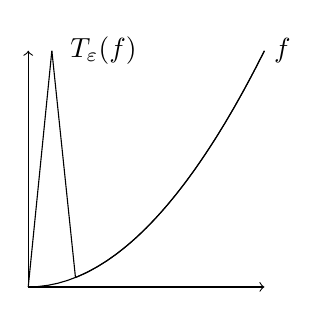
\begin{tikzpicture}[scale=3]
        \draw[->] (0, 0) -- (1, 0);
        \draw[->] (0, 0) -- (0, 1);

        \draw[domain=0:1, variable=\x] plot ({\x}, {\x^2}) node[right] {$f$};

        \draw (1/2, 1) node[left] {$T_\varepsilon(f)$};
        \draw[domain=0:0.1, variable=\x] plot ({\x}, {10 * \x});
        \draw[domain=0.1:0.2, variable=\x] plot ({\x}, {0.04 + (1 - 0.04) * (2 - 10 * \x)});
        \draw[domain=0.2:1, variable=\x] plot ({\x}, {\x^2});
      \end{tikzpicture}
    \end{Center}
  \end{figure}

  Define
  \begin{align*}
    T_\varepsilon(f)(x) \coloneqq \begin{cases}
      \frac x \delta_f, &0 \leq x < \delta_f \\
      f(\delta_f) + [1 - f(\delta_f)] (2 - \frac x {\delta_f}), &\delta_f \leq x < 2 \delta_f \\
      f(x), &x \geq 2 \delta_f,
    \end{cases}
  \end{align*}
  so that
  \begin{align*}
    \Norm{T_\varepsilon(f) - f}
    \geq
    T_\varepsilon(f) (\delta_f) - f(\delta_f)
    =
    1 - f(\delta_f)
    >
    1 - \varepsilon.
  \end{align*}

  Additionally, because $\delta_{T_\varepsilon(f)} < \delta_f$, we have that $f(\delta_{T_\varepsilon(f)}) < \varepsilon$ and
  \begin{align*}
    \Norm{T_\varepsilon(T_\varepsilon(f)) - f}
    \geq
    T_\varepsilon(T_\varepsilon(f)) (\delta_{T_\varepsilon(f)}) - f(\delta_{T_\varepsilon(f)})
    =
    1 - f(\delta_{T_\varepsilon(f)})
    >
    1 - \varepsilon.
  \end{align*}

  Thus, proceeding by induction, we see that for any $m = 1, 2, \ldots$
  \begin{align*}
    \Norm{T_\varepsilon^m(f) - f} > 1 - \varepsilon,
  \end{align*}
  where $T_\varepsilon^m$ denotes repeated application of $T_\varepsilon$.

  Consider the sequence
  \begin{align*}
    \{ T_\varepsilon^k(f) \}_{k=0}^\infty = \{ f, T_\varepsilon(f), T_\varepsilon(T_\varepsilon(f)), \ldots \}.
  \end{align*}

  We can easily see that the distance between any two elements of the sequence, say $T_\varepsilon^k(f)$ and $T_\varepsilon^{k+m}(f)$, is strictly greater that $1 - \varepsilon$, i.e.
  \begin{align*}
    \Norm{T_\varepsilon^k(f) - T_\varepsilon^{k+m}(f)}
    =
    \Norm{T_\varepsilon^k(f) - T_\varepsilon^m(T_\varepsilon^k(f))}
    >
    1 - \varepsilon.
  \end{align*}

  Hence $B_1$ cannot be covered by a finite $(1-\varepsilon)$-net and $\alpha(B_1) \geq 1 - \varepsilon$. Since $\varepsilon > 0$ can be made arbitrarily small, this implies that $\alpha(B_1) \geq 1$ and, because we already have the reverse inequality, $\alpha(B_1) = 1$.

  In the set $B_2$, the maximum distance between two functions is $\frac 1 2$, thus $\Diam(B_2) = \frac 1 2$ and $\alpha(B_2) \leq \frac 1 2$. We can then define an operator similar to $T_\varepsilon$ that creates \enquote{spikes} of height $\frac 1 2$ to prove the reverse inequality, obtaining
  \begin{align*}
    \alpha(B_2) = \frac 1 2.
  \end{align*}

  Finally, the set $B_3$ has diameter $\frac 2 3$ and hence $\alpha(B_3) = \frac 2 3$.

  The ball measure for $B_1$ satisfies the inequalities
  \begin{align*}
    \frac 1 2 \leq \beta(B_1) \leq 1.
  \end{align*}

  Additionally, $B_1$ is strictly contained in the ball centered in the constant function $\frac 1 2$ with radius $\frac 1 2$, which implies that $\beta(B_1) \leq \frac 1 2$, hence $\beta(B_1) = \frac 1 2$.

  For $B_2$ we have
  \begin{align*}
    \frac 1 4 \leq \beta(B_2) \leq \frac 1 2.
  \end{align*}

  Assume\LEM that for some $\varepsilon > 0$ the set $B_2$ can be covered by a finite set of balls with centers $\{ f_1, \ldots, f_n \} \subsetneq C([0, 1])$ and radius $\frac 1 2 - \varepsilon$.

  Because of continuity, we can find a radius $\delta > 0$ such that for all $f_k, k = 1, \ldots, n$ we have
  \begin{align*}
    x \in \left[\tfrac {1 - \delta} 2, \tfrac {1 + \delta} 2 \right] \implies \Abs{f_k(x) - f_k(\tfrac 1 2)} < \varepsilon.
  \end{align*}

  Consider the function
  \begin{align*}
    g(x) \coloneqq \begin{cases}
      0, &0 \leq x < \frac {1 - \delta} 2, \\
      \frac{2x + \delta - 1} {2\delta}, &\frac {1 - \delta} 2 \leq x \leq \frac {1 + \delta} 2, \\
      1, &\frac {1 + \delta} 2 < x \leq 1.
    \end{cases}
  \end{align*}

  \begin{figure}[ht]
    \begin{Center}
      \begin{tikzpicture}[scale=5]
        \draw[->] (0, 0) -- (1, 0);
        \draw[->] (0, 0) -- (0, 1);
        \draw[domain=0:4/10, thick, variable=\x] plot ({\x}, {0});
        \draw[domain=4/10:6/10, thick, variable=\x] plot ({\x}, {5 * \x - 2}) node[left] {$g$};
        \draw[domain=6/10:1, thick, variable=\x] plot ({\x}, {1});

        \draw[densely dotted] (0, 6/10) node[left] {$f_k(\frac 1 2) - \varepsilon$} -- (1, 6/10);
        \draw[densely dotted] (0, 8/10) node[left] {$f_k(\frac 1 2) + \varepsilon$} -- (1, 8/10);

        \draw[densely dotted] (4/10, 0) -- (4/10, 1);
        \draw (3/10, -1/10) node {$\frac {1 - \delta} 2$};
        \draw[densely dotted] (1/2, 0) -- (1/2, 1);
        \draw (1/2, -1/10) node {$\frac 1 2$};
        \draw[densely dotted] (6/10, 0) -- (6/10, 1);
        \draw (7/10, -1/10) node {$\frac {1 + \delta} 2$};

        \draw[domain=-1/10:1, dash dot, variable=\x] plot ({\x}, {2/10 + 1 / (1 + e^(5/3*(1-2*\x)))}) node[right] {$f_k$};
      \end{tikzpicture}
    \end{Center}
  \end{figure}

  If $f_k(\tfrac 1 2) \geq \frac 1 2$, then $f_k(\tfrac {1 - \delta} 2) > \tfrac 1 2 - \varepsilon$ and
  \begin{align*}
    \Norm{f_k - g} \geq f_k(\tfrac {1 - \delta} 2) - g(\tfrac {1 - \delta} 2) = f_k(\tfrac {1 - \delta} 2) > \tfrac 1 2 - \varepsilon.
  \end{align*}

  Analogously, if $f_k(\tfrac 1 2) < \frac 1 2$, then $f_k(\tfrac {1 + \delta} 2) < \tfrac 1 2 + \varepsilon$ and
  \begin{align*}
    \Norm{g - f_k} \geq g(\tfrac {1 + \delta} 2) - f_k(\tfrac {1 + \delta} 2) = 1 - f_k(\tfrac {1 + \delta} 2) > \tfrac 1 2 - \varepsilon.
  \end{align*}

  Thus, for every $k = 1, \ldots, n$ we have
  \begin{align*}
    \Norm{g - f_k} > \frac 1 2 - \varepsilon,
  \end{align*}
  i.e. $g$ in not contained in a ball of radius $\frac 1 2 - \varepsilon$ around any of the centers $f_1, \ldots, f_n$.

  Hence $\beta(B_2) \geq \frac 1 2$, which implies $\beta(B_2) = \frac 1 2$. Because of the inclusion $B_2 \subsetneq B_3 \subsetneq B_1$, we have
  \begin{align*}
    \frac 1 2 = \beta(B_2) \leq \beta(B_3) \leq \beta(B_1) = \frac 1 2,
  \end{align*}
  hence $\beta(B_3) = \frac 1 2$.
\end{proof}

\begin{theorem}\label{thm:noncompact_kuratowski_lemma}[Kuratowski lemma]\cite[exercise 7.4]{Deimling1985}
  Let $X$ be a Banach space and $\{ A_n \}_n$ be a decreasing sequence of nonempty closed subsets such that $\alpha(A_n) \to 0$. Then $A \coloneqq \bigcap_n A_n$ is nonempty and compact.
\end{theorem}
\begin{proof}
  The set $A$ is compact because it is closed as the intersection of closed sets and $\alpha(A) \leq \alpha(A_n) \to 0$, hence $\alpha(A) = 0$.

  It remains to show that $A$ is nonempty.
  Choose\AOC any sequence $\{ x_n \}_n$ where $x_n \in A_n$. Since any finite set is compact, we have that for any $k \geq 1$
  \begin{align*}
    \alpha(\{ x_n \}_{n \geq 1})
    =
    \max\{ \alpha(\{ x_n \}_{n < k}), \alpha(\{ x_n \}_{n \geq k}) \}
    =
    \alpha(\{ x_n \}_{n \geq k})
    \leq
    \alpha(A_k) \to 0,
  \end{align*}
  hence the set $\{ x_n \colon n \geq 1 \}$ is compact and thus sequentially compact. We can choose a convergent subsequence $\{ x_{n_k} \}_k$ of $\{ x_n \}_n$ whose limit lies in every $A_n$ (since they are closed) and, consequently, in their intersection $A$. So $A$ is nonempty.
\end{proof}


% Logic
\subsection{Languages}\label{subsec:languages}

Languages are used to define formulas for expressing the axioms of set theory\Tinyref{def:set_zfc}. Here, sets are used to formally define languages. This vicious cycle is left to logicians.

\begin{definition}\label{def:language}
  Given a set \( \Cal{A} \), called an \textbf{alphabet}, whose elements are called \textbf{symbols}, we define a \textbf{word} or \textbf{string} over \( \Cal{A} \) to be any tuple\Tinyref{def:cartesian_product} of symbols. Words are written simply as strings of symbols, that is, \( abc \) instead of \( (a, b, c) \). The empty word with no symbols is usually denoted by \( \varepsilon \).

  The set of all (finite) words over \( \Cal{A} \) is denoted by \( \Cal{A}^{*} \). The operation \( * \) is called the \textbf{Kleene star}. A \textbf{language} \( \Cal{L} \) is any subset of \( \Cal{A}^{*} \).

  We define two functions:
  \begin{align*}
    &\Len: \Cal{A}^{*} \to \BB{Z}^{\geq 0}
    &&\cdot: \Cal{A}^{*} \to \BB{Z}^{\geq 0}
    \\
    &\Len(w) \coloneqq \text{length of the tuple } w
    &&v \cdot w \coloneqq (v_1, \ldots, v_{\Len(v)}, w_1, \ldots, w_{\Len(w)}).
  \end{align*}

  The function \( v \cdot w \) is called \textbf{concatenation} and is usually denoted by juxtaposition. It is obviously associative.

  We say that \( p \) is a \textbf{prefix} of \( w \) if the first \( \Len(p) \) symbols of \( w \) are identical to those of \( p \), that is,
  \begin{equation*}
    w = (p_1, \ldots, p_{\Len(p)}, w_{\Len(p) + 1}, \ldots, w_{\Len(w)}).
  \end{equation*}

  \textbf{Suffixes} are defined analogously. We say that \( v \) is a \textbf{subword} of \( w \) if there exists a prefix \( p \) and a suffix \( s \) such that \( w = pvs \). We define the partial order\Tinyref{def:order/partial} \( v \leq w \iff v \) is a subword of \( w \).

  Evidently both prefixes and suffixes are subwords and \( v \leq w \iff \Len(v) \leq \Len(w) \).

  For convenience, we denote \textbf{runs of length \( n \)} of some letter \( a \) as \( a^n \), that is,
  \begin{align*}
    a^n \coloneqq \begin{cases}
      \varepsilon, &n = 0, \\
      a a^{n-1}, &n > 1.
    \end{cases}
  \end{align*}

  Thus we do not distinguish between the words \( aaabbaa \) and \( a^3 b^2 a^2 \).
\end{definition}

\begin{proposition}\label{thm:set_of_all_words_is_monoid}
  For any alphabet \( \Cal{A} \), the language \( (\Cal{A}^{*}, \cdot) \) is a monoid.
\end{proposition}

\subsection{Grammars}\label{subsec:grammars}

\begin{definition}\label{def:grammar}\cite[definition 2.2]{Sipser2013}
  Let \( \Cal{A} \) be some alphabet\Tinyref{def:language} and \( V, \Sigma \subseteq \Cal{A} \) be nonempty disjoint subsets of \( \Cal{A} \). We call elements of \( V \) \textbf{variables} and the elements of \( \Sigma \) \textbf{terminals}. Fix special \textbf{start symbol} \( S \in V \).

  We define a binary relation\Tinyref{def:relation} \( \to \) of \textbf{production rules} over \( (V \cup \Sigma)^* \), that is, rules are \enquote{transformations} that define how a language is \enquote{generated} starting from \( S \in V \) (see \cref{def:grammar_derivation} and \cref{ex:context_free_grammar/real_arithmetic}). As a shortcut, instead of listing individual rules with the same source as
  \begin{align*}
    &u \to v, \\
    &u \to w,
  \end{align*}
  we write
  \begin{equation*}
    u \to v | w.
  \end{equation*}

  Rules of the form \( u \to \sigma \) where \( \sigma \in \Sigma \) are called \textbf{terminal rules}.

  We call the tuple \( G \coloneqq (V, \Sigma, R, S) \) a \textbf{formal grammar}. If every production rule has only a single variable for a source, we say that the grammar is a \textbf{context-free grammar}.
\end{definition}

\begin{note}\label{note:grammar_symbol_case}
  It is a common convention to denote variables with uppercase letters and terminals with lowercase letters. Lowercase letters are also used, however, for words in \( (V \cup \Sigma)^* \).
\end{note}

\begin{definition}\label{def:grammar_derivation}\cite[104,108]{Sipser2013}
  Fix a word \( pvs \) (\enquote{\( p \)} stands for \enquote{prefix} and \enquote{\( s \)} stands for \enquote{suffix}). If \( u \to v \) is a production rule, we say that \( pvs \) \textbf{yields} the word \( pws \) and write \( pvs \implies pws \).

  We say that \textbf{\( u \) derives \( v \)} and write \( u \Derives v \) if there exists a finite sequence of words \( u_1, \ldots, u_n \) such that
  \begin{equation*}
    u \implies u_1 \implies \ldots \implies u_n \implies v.
  \end{equation*}

  If on every step of the derivation the leftmost (resp. rightmost) variable is replaced, we say that it is a \textbf{leftmost (resp. rightmost) derivation}.

  Define the \textbf{language of the grammar} to be
  \begin{equation*}
    \Cal{L}(G) \coloneqq \{ w \in \Sigma^* \colon S \implies w \},
  \end{equation*}
  that is, all words that can be derived from \( S \) and contains only terminals.

  We also say that strings in \( \Cal{L}(G) \) are \textbf{generated by the grammar \( G \)}.
\end{definition}

\begin{definition}\label{def:ambiguous_grammar}\cite[definition 2.7]{Sipser2013}
  Let \( G \) be a grammar. We say that the word \( w \) can be derived \textbf{unambiguously} if there exists a unique leftmost derivation from \( S \). Otherwise we say that \( w \) is generated \textbf{ambiguously} and that the grammar itself is \textbf{ambiguous}.
\end{definition}

\begin{example}\label{ex:context_free_grammar/real_arithmetic}
  We will define a grammar for addition on natural numbers\Tinyref{def:natural_numbers_zfc}. Note that we only consider the number in \( \BB{N} \) only as symbols, not as the numbers themselves.

  Let \( V \coloneqq \{ A \} \) and \( \Sigma \coloneqq \BB{N} \cup \{ +, \cdot, (, ) \} \). Define the rules:
  \begin{itemize}
    \item for each natural number \( n \), define the rule \( A \to n \).
    \item \( A \to (A + A) \)
  \end{itemize}

  Choose the starting symbol to be the only symbol \( x \) in \( V \). Then the grammar can produce the arithmetic expression \( ((1 + 2) + 3) \) by applying the rules
  \begin{equation*}
    \begin{mplibcode}
      u := 2cm;

      beginfig(1);
        input metapost/diagrams;

        n1 := thelabel("$A$", origin);
        n2 := thelabel("$(A + A)$", (0, -1) * u);
        n3 := thelabel("$3$", (1, -2) * u);
        n4 := thelabel("$(A + A)$", (-1, -2) * u);
        n5 := thelabel("$1$", (-2, -3) * u);
        n6 := thelabel("$2$", (0, -3) * u);

        a1 := straight_arrow(n1, n2);
        a2 := straight_arrow(n2, n3);
        a3 := straight_arrow(n2, n4);
        a4 := straight_arrow(n4, n5);
        a5 := straight_arrow(n4, n6);

        draw_nodes(n);
        draw_arrows(a);

        label.lft("$A \to (A + A$)", midpoint of a1);
        label.urt("$A \to 3$", midpoint of a2);
        label.ulft("$A \to (A + A)$", midpoint of a3);
        label.ulft("$A \to 1$", midpoint of a4);
        label.urt("$A \to 2$", midpoint of a5);
      endfig;
    \end{mplibcode}
  \end{equation*}

  Note that the grammar is unambiguous because of the parentheses. If we omit the parentheses, it will no longer be unambiguous since \( 1 + 2 + 3 \) can be derived by both
  \begin{equation*}
    \begin{mplibcode}
      u := 2cm;

      beginfig(1);
        input metapost/diagrams;

        n1 := thelabel("$A$", origin);
        n2 := thelabel("$A + A$", (0, -1) * u);
        n3 := thelabel("$1$", (-1, -2) * u);
        n4 := thelabel("$A + A$", (1, -2) * u);
        n5 := thelabel("$2$", (0, -3) * u);
        n6 := thelabel("$3$", (2, -3) * u);

        a1 := straight_arrow(n1, n2);
        a2 := straight_arrow(n2, n3);
        a3 := straight_arrow(n2, n4);
        a4 := straight_arrow(n4, n5);
        a5 := straight_arrow(n4, n6);

        draw_nodes(n);
        draw_arrows(a);

        label.lft("$A \to A + A$", midpoint of a1);
        label.ulft("$A \to 1$", midpoint of a2);
        label.urt("$A \to A + A$", midpoint of a3);
        label.ulft("$A \to 2$", midpoint of a4);
        label.urt("$A \to 3$", midpoint of a5);
      endfig;
    \end{mplibcode}
    \hspace{1cm}
    \begin{mplibcode}
      u := 2cm;

      beginfig(1);
        input metapost/diagrams;

        n1 := thelabel("$A$", origin);
        n2 := thelabel("$A + A$", (0, -1) * u);
        n3 := thelabel("$3$", (1, -2) * u);
        n4 := thelabel("$A + A$", (-1, -2) * u);
        n5 := thelabel("$1$", (-2, -3) * u);
        n6 := thelabel("$2$", (0, -3) * u);

        a1 := straight_arrow(n1, n2);
        a2 := straight_arrow(n2, n3);
        a3 := straight_arrow(n2, n4);
        a4 := straight_arrow(n4, n5);
        a5 := straight_arrow(n4, n6);

        draw_nodes(n);
        draw_arrows(a);

        label.lft("$A \to A + A$", midpoint of a1);
        label.urt("$A \to 3$", midpoint of a2);
        label.ulft("$A \to A + A$", midpoint of a3);
        label.ulft("$A \to 1$", midpoint of a4);
        label.urt("$A \to 2$", midpoint of a5);
      endfig;
    \end{mplibcode}
  \end{equation*}
\end{example}
\begin{proof}
  We will show that \( G \) is unambiguous. Let \( w \) be a word in \( \Cal{L}(G) \). We explicitly build the derivation of \( w \):
  \begin{itemize}
    \item If \( \Len(w) = 1 \), then \( w \in \BB{N} \) and the word has been generated by the single rule \( A \to w \).
    \item If \( \Len(w) > 1 \), then \( w \) is necessarily enclosed in parentheses. Let \( w = ( \sigma_0 \ldots \sigma_m ) \) be the symbols of \( w \). Because of the parentheses, the only possibility for \( \sigma_0 \ldots \sigma_m \) is that it consists of two words in \( \Cal{L}(G) \) with an operation symbol \( \circ \in \{ +, \cdot \} \) between them. Let \( k \) be the index of the operator, that is, the index such that \( \sigma_1 \ldots \sigma_{k-1} \) and \( \sigma_{k+1} \ldots \sigma_m \) both belong to \( \Cal{L}(G) \).

    The derivation of \( w \) is then given by \( A \to (A \sigma_k A) \), followed by applying the same algorithm to the word \( \sigma_1 \ldots \sigma_{k-1} \), followed by applying the same algorithm to the word \( \sigma_1 \ldots \sigma_{k+1} \).
  \end{itemize}
\end{proof}

\section{Propositional logic}\label{sec:propositional_logic}

Propositional logic is a simple framework for describing relationships between statements. It is sometimes called boolean logic because of~\cref{thm:propositional_logic_boolean_algebra}.

\begin{definition}\label{def:propositional_logic_language}\cite[12]{Nerode2012}
  The language\Tinyref{def:language} of propositional logic consists of \ul{propositional formulas}, which are certain well-formed words over the alphabet consisting of
  \begin{defenum}
    \item\label{def:propositional_logic_language/prop} A nonempty set $\Bold{Prop}$ of \ul{propositional variables}.
    \item\label{def:propositional_logic_language/negation} The \ul{negation} symbol $\neg$.
    \item\label{def:propositional_logic_language/connectives} The \ul{propositional connectives} \ul{conjunction} $\land$ and \ul{disjunction} $\lor$ (we may additionally define other connectives like $\implies$ and $\iff$, however this will only clutter our formal language and make proofs more difficult).
    \item\label{def:propositional_logic_language/parentheses} Parentheses $($ and $)$ for defining the order of operations unambiguously.
  \end{defenum}

  The propositional formulas $\Cal{F}_B$ are defined inductively as
  \begin{itemize}
    \item the variables in $\Bold{Prop}$ are formulas.
    \item if $\varphi$ is a formula, then $\neg \varphi$ is a formula.
    \item if $\varphi$ and $\psi$ are formulas, so are $(\varphi \land \psi)$ and $(\varphi \lor \psi)$.
  \end{itemize}

  Furthermore, we are able to determine every formula's constituent parts uniquely.

  If $\varphi$ and $\psi$ are formulas and $\psi$ is a subword of $\varphi$, we say that $\psi$ is a \ul{subformula} of $\varphi$.
\end{definition}

\begin{definition}\label{def:conjunctive_normal_form}
  We define \ul{literals} to either be propositional variables $L = P$ or negations $L = \neg P$ of propositional variables.

  We define \ul{disjuncts} (resp. \ul{conjuncts}) to be finite disjunctions (resp. conjunctions) of literals, i.e.
  \begin{align*}
    (L_1 \lor (L_2 \lor (\ldots \lor L_n) \ldots ).
  \end{align*}

  We say that a propositional formula $\varphi$ is in \ul{conjunctive (resp. disjunctive) normal form (CNF)} if $\varphi$ is a finite conjunction of disjunctions (resp. finite disjunction of conjunctions).
\end{definition}

\begin{proposition}\label{thm:conjunctive_normal_form_reduction}
  Every propositional formula $\varphi$ is Boolean equivalent\Tinyref{def:propositional_interpretation} to a formula in conjunctive normal form\Tinyref{def:conjunctive_normal_form}.
\end{proposition}
\begin{proof}
  We define the negation function
  \begin{align*}
    n(\varphi) \coloneqq \begin{cases}
      \neg P,                                                   &\varphi = P \in \Bold{Prop} \\
      \psi,                                                     &\varphi = \neg \psi \\
      n(\psi) \land n(\theta),                                  &\varphi = \psi \lor \theta \\
      n(\psi) \lor n(\theta),                                   &\varphi = \psi \land \theta \\
    \end{cases}
  \end{align*}

  and the reduction function
  \begin{align*}
    r(\varphi) \coloneqq \begin{cases}
      \varphi,                                                  &\varphi \in \Bold{Prop} \\
      n(r(\psi)),                                               &\varphi = \neg \psi \\
      r(\psi) \lor r(\theta),                                   &\varphi = \psi \lor \theta \\
      r(\psi) \land r(\theta),                                  &\varphi = \psi \land \theta \\
      (r(\psi) \lor r(\theta)) \land (r(\psi) \lor r(\kappa)),  &\varphi = \psi \lor (\theta \land \kappa) \\
    \end{cases}
  \end{align*}

  Given a formula $\varphi$, the function $r(\varphi)$ gives a formula in CNF.
\end{proof}

\begin{definition}\label{def:truth_functions}
  We define the following auxiliary functions using truth tables
  \begin{center}
    \begin{tabular}{c | c || c c | c c}
      $x$    & $H_\neg$ & $x$    & $y$    & $H_\lor$ & $H_\land$ \\
      \hline
      $\top$ & $\bot$   & $\top$ & $\top$ & $\top$   & $\top$    \\
      $\bot$ & $\top$   & $\top$ & $\bot$ & $\bot$   & $\top$    \\
             &          & $\bot$   & $\top$ & $\bot$ & $\top$    \\
             &          & $\bot$   & $\bot$ & $\bot$ & $\bot$
    \end{tabular}
  \end{center}

  Note that, as operations over the set $\{ \top, \bot \}$, $H_\lor$ and $H_\land$ are both associative and commutative.
\end{definition}

\begin{definition}\label{def:propositional_interpretation}
  A \ul{propositional interpretation} is a function $I: \Bold{Prop} \to \{ \top, \bot \}$.

  We define interpretation for formulas inductively as
  \begin{align*}
    \varphi[I] \coloneqq \begin{cases}
      I(P),                        &\varphi = P \in \Bold{Prop} \\
      H_\neg(\psi[I]),             &\varphi = \neg \psi         \\
      H_\land(\psi[I], \theta[I]), &\varphi = \psi \land \theta \\
      H_\lor(\psi[I], \theta[I]),  &\varphi = \psi \lor \theta.
    \end{cases}
  \end{align*}

  We say that
  \begin{defenum}
    \item\label{def:propositional_interpretation/model} $I$ is a Boolean model of $\varphi$ and write $I \models_B \varphi$ if $\varphi[I] = \top$.
    \item\label{def:propositional_interpretation/tautology} If all interpretations are models for $\varphi$, we say that $\varphi$ is a \ul{tautology}.
    \item\label{def:propositional_interpretation/contradiction} If no interpretation is a model for $\varphi$, we say that $\varphi$ is a \ul{contradiction}.
    \item\label{def:propositional_interpretation/equivalence} $\varphi$ and $\psi$ are \ul{Boolean equivalent} and write $\varphi \equiv_B \psi$ if $\varphi[I] = \psi[I]$ for any interpretation $I$.
  \end{defenum}
\end{definition}

\begin{proposition}\label{thm:boolean_equivalence_relation}
  The Boolean equivalence\Tinyref{def:propositional_interpretation} $\equiv_B$ is an equivalence relation on the set $\Cal{F}_B$ of propositional formulas.
\end{proposition}

\begin{theorem}\label{thm:propositional_logic_boolean_algebra}
  The quotient set\Tinyref{def:order/equivalence} of propositional formulas $\Cal{F}_B / \cong$ forms a boolean algebra\Tinyref{def:boolean_algebra} with
  \begin{itemize}
    \item top being the equivalence class of tautologies
    \item bottom being the equivalence class of contradictions
    \item joins given by disjunctions $\lor$ of any representatives of the equivalence classes
    \item meets given by conjunctions $\land$
    \item complements given by negation $\neg$
  \end{itemize}
\end{theorem}
\begin{proof}
  See \cref{note:infinite_join_meet} about handling infinitary joins and meets. Once we prove \ref{def:binary_join_meet/associativity}, \ref{def:binary_join_meet/commutativity} and \ref{def:binary_join_meet/absorption}, we can define a partial order on $\Cal{F}_B / \cong$ that allows us to extend $\lor$ and $\land$ to handle infinite arguments.

  \begin{description}
    \item[\ref{def:binary_join_meet/associativity}] The functions\Tinyref{def:truth_functions} $H_\lor$ and $H_\land$ are associative, hence the lattice operations are associative.
    \item[\ref{def:binary_join_meet/commutativity}] The proof is analogous to \ref{def:binary_join_meet/associativity}.
    \item[\ref{def:binary_join_meet/absorption}] Let $\varphi$ and $\psi$ be propositional formulas and $I$ be a propositional interpretation. Then
    \begin{center}
      \begin{tabular}{c c | c | c}
        $\varphi[I]$ & $\psi[I]$ & $H_\land(\psi[I], \varphi[I])$ & $H_\lor(\varphi[I], H_\land(\psi[I], \varphi[I]))$ \\
        \hline
        $\top$       & $\top$    & $\top$                         & $\top$ \\
        $\top$       & $\bot$    & $\bot$                         & $\top$ \\
        $\bot$       & $\top$    & $\bot$                         & $\bot$ \\
        $\bot$       & $\bot$    & $\bot$                         & $\bot$
      \end{tabular}
    \end{center}
    hence $\varphi[I] = H_\lor(\varphi[I], H_\land(\psi[I], \varphi[I]))$.

    The proof of the dual law is analogous.

    \item[\ref{def:distributive_lattice/distributivity}] Let $\varphi$, $\psi$ and $\theta$ be propositional formulas and $I$ be a propositional interpretation. Then
    \begin{center}
      \begin{tabular}{c c c | c | c}
        $\varphi[I]$ & $\psi[I]$ & $\theta[I]$ & \small{$H_\land(\varphi[I], H_\lor(\psi[I], \theta[I]))$} & \small{$H_\lor(H_\land(\varphi[I], \psi[I]), H_\land(\varphi[I], \theta[I]))$} \\
        \hline
        $\top$       & $\top$    & $\top$      & $\top$                                            & $\top$ \\
        $\top$       & $\top$    & $\bot$      & $\top$                                            & $\top$ \\
        $\top$       & $\bot$    & $\top$      & $\top$                                            & $\top$ \\
        $\top$       & $\bot$    & $\bot$      & $\bot$                                            & $\bot$ \\
        $\bot$       & $\top$    & $\top$      & $\bot$                                            & $\bot$ \\
        $\bot$       & $\top$    & $\bot$      & $\bot$                                            & $\bot$ \\
        $\bot$       & $\bot$    & $\top$      & $\bot$                                            & $\bot$ \\
        $\bot$       & $\bot$    & $\bot$      & $\bot$                                            & $\bot$
      \end{tabular}
    \end{center}
  \end{description}

  The join and meet induce the partial order $\varphi \leq \psi \iff \varphi \lor \psi \equiv \psi$.

  \begin{description}
    \item[\ref{def:lattice/top}] Fix an interpretation $I$. A formula $\omega$ should belong to the supremum $\sup \Cal{F}_B$ if and only if $\varphi \lor \omega \equiv \omega$ for any formula $\varphi \in \Cal{F}_B$. If $\varphi$ is a tautology, $\varphi[I] = \top$ and thus
    \begin{align*}
      (\varphi \lor \omega)[I] \coloneqq H_\lor(\varphi[I], \omega[I]) = \top.
    \end{align*}

    It follows that $\omega[I] = \top$. Since the interpretation $I$ was arbitrary, $\omega$ is also a tautology. Hence the top element is the equivalence class of all tautologies.

    \item[\ref{def:lattice/bottom}] The proof is analogous to \ref{def:lattice/top}.
  \end{description}
\end{proof}

\subsection{First order logic}\label{subsec:first_order_logic}

\begin{definition}\label{def:first_order_language}\cite[definition 2.1]{Nerode2012}
  The idea of first-order logic (FOL) is to create a formal language whose semantics (given by structures) support boolean operations and can quantify over all elements of an ambient universe. Unlike in propositional logic\Tinyref{subsec:propositional_logic}, there are many FOL languages.

  The alphabet for a \textbf{first-order predicate language}\Tinyref{def:language} \( \Cal{L} \) consists of:
  \begin{description}
    \item[Logical symbols]
    \mbox{}
    \begin{enumerate}
      \item A countable alphabet of variables \( \Bold{Var}_{\Cal{L}} \), usually denoted by \( x_0, x_1, \ldots \) or \( x, y, z \).

      \item Certain propositional operations:
      \begin{description}
        \RItem{def:propositional_logic_language/constants} \( \top \) and \( \bot \) - zero-arity operations
        \RItem{def:propositional_logic_language/negation} \( \neg \) - unary operation
        \RItem{def:propositional_logic_language/connectives} \( \Sigma = \{ \land, \lor, \implies, \iff, \downarrow, \uparrow \} \) - binary operations
      \end{description}

      \item Quantifiers
      \begin{itemize}
        \item \( \forall \) (universal quantifier)
        \item \( \exists \) (existential quantifier)
      \end{itemize}

      \item Parentheses \( ( \) and \( ) \) for defining the order of operations unambiguously (see \cref{remark:propositional_formula_parentheses}).

      \item Optionally, an equality symbol \( \doteq \).
    \end{enumerate}

    \item[Non-logical symbols]
    \mbox{}
    \begin{enumerate}
      \item A set of functional symbols, \( \Bold{Func}_{\Cal{L}} \), whose elements are usually denoted by \( f_0, f_1, \ldots \) or \( f, g, h \). Each functional symbol has an associated natural number called its \textbf{arity}, denoted by \( \#_{\Cal{L}} f \). Functional symbols with a zero arity are called \textbf{constants}.

      \item A set of predicate symbols, \( \Bold{Pred}_{\Cal{L}} \), whose elements are usually denoted by \( p_0, p_1, \ldots \) or by symbols like \( \oplus \) or \( \circ \). Predicate symbols also have an associated arity. Predicate symbols with zero arity are called \textbf{propositional variables}.
    \end{enumerate}
  \end{description}
\end{definition}

\begin{example}\label{ex:algebraic_theory_language}\cite[remark 2.1.4]{Leinster2014}
  Most algebraic structures (with the notable exception of fields) can be defined as first-order languages with equality, no predicates and a set of functional symbols called \textbf{algebraic operations}.
  \begin{itemize}
    \item Group theory\Tinyref{subsec:groups} has
    \begin{itemize}
      \item one zero-arity operation called its identity element \( e \)
      \item one unitary operation \( (\cdot)^{-1} \) called the inverse element
      \item one binary operation \( \oplus \) called the group operation
    \end{itemize}

    \item Linear algebra\Tinyref{subsec:vector_spaces} has
    \begin{itemize}
      \item one zero-arity operation called its zero element \( 0 \)
      \item one binary operation \( + \) called vector sum
      \item for every scalar \( \lambda \) in the underlying field, a unitary operation \( \lambda \cdot \) called scalar multiplication by \( \lambda \)
    \end{itemize}
  \end{itemize}
\end{example}

\begin{definition}\label{def:first_order_term}\cite[definition 2.2]{Nerode2012}
  Given a FOL language \( \Cal{L} \), the set \( \Cal{T}_{\Cal{L}} \) of terms is defined by structural induction as
  \begin{itemize}
    \item Each variable is a term
    \item If \( \tau_1, \ldots, \tau_n \) are terms and \( f \) is a functional symbol with arity \( n \), then the following word is also a term:
    \begin{equation*}
      f(\tau_1, \ldots, \tau_n)
    \end{equation*}
  \end{itemize}

  In particular, constants are also terms.

  Furthermore, the grammar of first-order terms is unambiguous (see \cref{thm:first_order_formulas_are_unambiguous}).

  For each term \( \tau \), we define its variables as
  \begin{align*}
    \Bold{Free}(\tau) \coloneqq \begin{cases}
      x,                                                        &\tau = x \in \Bold{Var}_{\Cal{L}}, \\
      \Bold{Free}(\tau_1) \cup \ldots \cup \Bold{Free}(\tau_n), &\tau = f(\tau_1, \ldots, \tau_n).
    \end{cases}
  \end{align*}
\end{definition}

\begin{definition}\label{def:first_order_formula}\cite[definition 2.5]{Nerode2012}
  Given a FOL language \( \Cal{L} \), we define the set of atomic formulas inductively as
  \begin{itemize}
    \item Both \( \top \) and \( \bot \) are atomic formulas.
    \item If \( p \) is an n-ary predicate symbol and if \( \tau_1, \ldots, \tau_n \) are terms, then \( p(\tau_1, \ldots, \tau_n) \) is an atomic formula.
    \item If \( \Cal{L} \) has an equality symbol and if \( \tau_1, \tau_2 \) are terms, then \( (\tau_1 \doteq \tau_2) \) is an atomic formula.
  \end{itemize}

  The set \( \Cal{F}_{\Cal{L}} \) of predicate formulas is then defined as
  \begin{itemize}
    \item All atomic formulas are formulas
    \item If \( \varphi \) is a formula, its negation \( \neg \varphi \) is also a formula
    \item If \( \varphi \) and \( \psi \) are formulas, then \( (\varphi \circ \psi), \circ \in \Sigma \)\Tinyref{def:propositional_logic_language}, are also formulas
    \item If \( \varphi \) is a formula and \( x \) is a variable, then the following are also formulas:
    \begin{itemize}
      \item \( \forall x \varphi \)
      \item \( \exists x \varphi \)
    \end{itemize}
  \end{itemize}

  Furthermore, the grammar of first-order formulas is unambiguous (see \cref{thm:first_order_formulas_are_unambiguous}).

  For each formula \( \varphi \), we define its free and bound variables as
  \begin{align*}
    \Bold{Free}(\varphi) \coloneqq \begin{cases}
      \varnothing,                                              &\varphi \in \{ \top, \bot \} \\
      \Bold{Free}(\tau_1) \cup \ldots \cup \Bold{Free}(\tau_n), &\varphi = p(\tau_1, \ldots, \tau_n) \\
      \Bold{Free}(\tau_1) \cup \Bold{Free}(\tau_2),             &\varphi = (\tau_1 \doteq \tau_2), \\
      \Bold{Free}(\psi),                                        &\varphi = \neg \psi, \\
      \Bold{Free}(\psi_1) \cup \Bold{Free}(\psi_2),             &\varphi = \psi_1 \circ \psi_2, \circ \in \Sigma, \\
      \Bold{Free}(\psi) \setminus \{ x \},                      &\varphi = Q x \psi, Q \in \{ \forall, \exists \}
    \end{cases}
  \end{align*}
  and
  \begin{align*}
    \Bold{Bound}(\varphi) \coloneqq \begin{cases}
      \varnothing,                                              &\varphi \in \{ \top, \bot \} \\
      \varnothing,                                              &\varphi = p(\tau_1, \ldots, \tau_n) \\
      \varnothing,                                              &\varphi = (\tau_1 \doteq \tau_2), \\
      \Bold{Bound}(\psi),                                       &\varphi = \neg \psi, \\
      \Bold{Bound}(\psi_1) \cup \Bold{Bound}(\psi_2),           &\varphi = \psi_1 \circ \psi_2, \circ \in \Sigma, \\
      \Bold{Bound}(\psi) \cup \{ x \},                          &\varphi = Q x \psi, Q \in \{ \forall, \exists \}.
    \end{cases}
  \end{align*}

  A formula is called \textbf{closed} if it has no bound variables.

  If a formula \( \varphi \) has free variables \( \Bold{Free} = \{ x_1, \ldots, x_n \} \), a common convention is to write it as
  \begin{equation*}
    \varphi(x_1, \ldots, x_n).
  \end{equation*}

  This highlights that formulas with free variables can act as predicates, however their semantics are completely determined by the actual predicates.

  Analogously to \cref{def:propositional_theory}, we define a \textbf{first-order theory} to be a set of formulas along with any additional axioms, like the ones from \cref{remark:minimal_first_order_language} and \cref{remark:first_order_equality}.
\end{definition}

\begin{proposition}\label{thm:first_order_formulas_are_unambiguous}
  The grammar\Tinyref{def:grammar}
  \begin{displaymath}
    \begin{aligned}
      &\Theta \to v,                                          && v \in \Bold{Var} \\
      &\tau \to \Theta,                                       && \\
      &\tau \to f(\tau, \ldots, \tau),                        && f \in \Bold{Func} \text{ is an } n-\text{ary functional symbol} \\
      &\Phi \to \top \;|\; \bot                               && \\
      &\Phi \to p(\tau, \ldots, \tau),                        && p \in \Bold{Pred} \text{ is an } n-\text{ary predicate symbol} \\
      &\Phi \to (\tau \doteq \tau)                            && \\
      &\Phi \to \neg \Phi                                     && \\
      &\Phi \to (\Phi \circ \Phi),                            && \circ \in \Sigma \\
      &\Phi \to \forall \Theta \Phi \;|\; \exists \Theta \Phi && \\
    \end{aligned}
  \end{displaymath}
  of first order formulas\Tinyref{def:first_order_formula} is unambiguous\Tinyref{def:ambiguous_grammar}.
\end{proposition}
\begin{proof}
  The proof is more complicated but similar to \cref{thm:propositional_formulas_are_unambiguous}.
\end{proof}

\begin{remark}\label{remark:minimal_first_order_language}
  As in \cref{remark:minimal_propositional_language}, to avoid redundancy in definitions and proofs, we can use the Pierce arrow \( \downarrow \) to define the constants, negation and all other connectives by adding additional axioms to every theory.
\end{remark}

\begin{remark}\label{remark:first_order_equality}\cite[definition 5.1]{Nerode2012}
  Equality is a concept that implies that two objects are completely indistinguishable. Let \( \Cal{L} \) be a first-order language with an equality symbol. In order to make equality behave as expected, we want the following formulas to be added implicitly to any theory:

  \begin{defenum}
    \DItem{remark:first_order_equality/reflexivity} for any \( x \in \Bold{Var}_{\Cal{L}} \), add the formula \( (x \doteq x) \).
    \DItem{remark:first_order_equality/equality} for any four variables \( x_1, x_2, y_1, y_2 \), add
    \begin{equation*}
      ((x_1 \doteq y_1) \land (x_2 \doteq y_2)) \implies ((x_1 \doteq x_2) \iff (y_1 \doteq y_2)).
    \end{equation*}

    \DItem{remark:first_order_equality/functions} for any \( n \)-ary function \( f \) and any set \( \{ x_1, \ldots, x_n, y_1, \ldots, y_n \} \subseteq \Bold{Var} \), add
    \begin{equation*}
      ((x_1 \doteq y_1) \land \ldots \land (x_n \doteq y_n)) \implies (f(x_1, \ldots, x_n) \doteq f(y_1, \ldots, y_n)).
    \end{equation*}

    \DItem{remark:first_order_equality/predicates} analogously, for any \( n \)-ary predicate \( p \), add
    \begin{equation*}
      ((x_1 \doteq y_1) \land \ldots \land (x_n \doteq y_n)) \implies (p(x_1, \ldots, x_n) \iff p(y_1, \ldots, y_n)).
    \end{equation*}
  \end{defenum}

  In particular, this ensures that equality is an equivalence relation (see \cref{thm:first_order_equality_equivalence_relation}).
\end{remark}

\begin{definition}\label{def:first_order_substition}
  Let \( \varphi \) be a first-order formula with a free variable \( y \) and \( \rho \) be a term. We define the \textbf{substitions}
  \begin{align*}
    \tau[y \to \rho] &\coloneqq \begin{cases}
      \rho,                                              &\tau = y, \\
      x,                                                 &\tau = x \in \Bold{Var}_{\Cal{L}} \setminus \{ y \}, \\
      f(\tau_1[y \to \rho], \ldots, \tau_n[y \to \rho]), &\tau = f(\tau_1, \ldots, \tau_n).
    \end{cases}
    \\
    \varphi[y \to \rho] &\coloneqq \begin{cases}
      \varphi,                                           &\varphi \in \{ \top, \bot \} \\
      p(\tau_1[y \to \rho], \ldots, \tau_n[y \to \rho]), &\varphi = p(\tau_1, \ldots, \tau_n) \\
      (\tau_1[y \to \rho] \doteq \tau_2[y \to \rho]),    &\varphi = (\tau_1 \doteq \tau_2), \\
      \neg \psi[y \to \rho],                             &\varphi = \neg \psi, \\
      \psi_1[y \to \rho] \circ \psi_2[x \to \rho],       &\varphi = \psi_1 \circ \psi_2, \circ \in \Sigma, \\
      Q x \psi[y \to \rho],                              &\varphi = Q x \psi, Q \in \{ \forall, \exists \}, x \not\in \Bold{Free}(\rho), \\
      Q x \psi[y \to \rho[x \to z]],                     &\varphi = Q x \psi, Q \in \{ \forall, \exists \}, x \in \Bold{Free}(\rho)
    \end{cases}
  \end{align*}
  where in the last step \( z \in \Bold{Var} \setminus \Bold{Free}(\rho) \).

  We define \textbf{simultaneous substition of \( y_1, \ldots, y_n \) with \( \rho_1, \ldots, \rho_n \)} analogously to \cref{def:propositional_substition}.
\end{definition}

\begin{definition}\label{def:first_order_structure}\cite[definition 4.1]{Nerode2012}
  Fix a FOL language \( \Cal{L} \). A \textbf{structure} for \( \Cal{L} \) consists of:
  \begin{enumerate}
    \item A nonempty set \( A \).
    \item A binary relation\Tinyref{def:relation} \( I(\doteq) \subseteq A^2 \) called the \textbf{interpretation of the equality}.
    \item For every \( n \)-ary function symbol \( f \), a function\Tinyref{def:function} \( I(f): A^n \to A \) called the \textbf{interpretation of \( f \)}.
    \item For every \( n \)-ary predicate \( p \), an n-ary relation\Tinyref{def:relation} \( I(p) \subseteq A^n \) called the \textbf{interpretation of \( p \)}, i.e. all tuples of values that satisfy the predicate within the structure.
  \end{enumerate}
\end{definition}

\begin{definition}\label{def:first_order_evaluation}
  Fix a structure \( \Cal{A} = (A, I) \) for a FOL language \( \Cal{L} \). An \textbf{evaluation for the variables of \( \Cal{L} \)} is any function \( v: \Bold{Var}_{\Cal{L}} \to A \).

  For every variable \( x \) and every universe element \( a \in A \) we also define the \textbf{modified at \( x \) with \( a \) evaluation}
  \begin{align*}
    v_a^x(y) \coloneqq \begin{cases}
      a,    &y = x, \\
      v(y), &y \neq x.
    \end{cases}
  \end{align*}

  Inductively,
  \begin{equation*}
    v_{a_1, \ldots, a_n}^{x_1, \ldots, x_n}(y) \coloneqq ((v_{a_1}^{x_1})_{a_2}^{x_2})\cdots_{a_n}^{x_n}.
  \end{equation*}

  This allows us to define semantics for all terms:
  \begin{align*}
    \tau[v] \coloneqq \begin{cases}
      v(x),                               &\tau = x \in \Bold{Var}_{\Cal{L}}, \\
      I(f)(\tau_1[v], \ldots, \tau_n[v]), &\tau = f(\tau_1, \ldots, \tau_n).
    \end{cases}
  \end{align*}
  and all formulas:
  \begin{align*}
    \varphi[v] \coloneqq \begin{cases}
      T,                                                &\varphi = \top, \\
      F,                                                &\varphi = \bot, \\
      (\tau_1[v], \tau_2[v]) \in I(\doteq),             &\varphi = (\tau_1 \doteq \tau_2), \\
      (\tau_1[v], \ldots, \tau_n[v]) \in I(p),          &\varphi = p(\tau_1, \ldots, \tau_n), \\
      H_\neg(\psi[v]),                                  &\varphi = \neg \psi, \\
      H_\circ(\psi_1[v], \psi_2[v]),                    &\varphi = \psi_1 \circ \psi_2, \circ \in \Sigma, \\
      \text{for all } a \in A, \psi[v_a^x] = T,         &\varphi = \forall x \psi, \\
      \text{there exists } a \in A: \psi[v_a^x] = T,    &\varphi = \exists x \psi.
    \end{cases}
  \end{align*}

  If \( \varphi[v] = T \), we say that \textbf{\( \varphi \) is true in \( \Cal{A} \) under the evaluation \( v \)} and we write \( \Cal{A} \models_v \varphi \). If \( \varphi \) is true in \( \Cal{A} \) under every evaluation, we say that \textbf{\( \varphi \) is true or valid in \( \Cal{A} \)} and we write \( \Cal{A} \models \varphi \).

  Given a formula \( \varphi(x_1, \ldots, x_n) \), we write
  \begin{equation*}
    \varphi[a_1, \ldots, a_n] \coloneqq \varphi(x_1, \ldots, x_n)[v_{a_1, \ldots, a_n}^{x_1, \ldots, x_n}].
  \end{equation*}

  We also apply this notation for terms.
\end{definition}

\begin{definition}\label{def:first_order_model}\cite[definition 4.4]{Nerode2012}
  A \textbf{model} for a first-order theory \( \Gamma \) in the FOL language \( \Cal{L} \) is a structure \( \Cal{A} \) such that there exists a single evaluation \( v \) so that for every formula \( \gamma \in \Gamma \), we have \( \Cal{A} \models_v \gamma \). We write \( \Cal{A} \models_v \Gamma \) or simply \( \Cal{A} \models \Gamma \).
\end{definition}

\begin{definition}\label{def:first_order_consistency}
  A first-order theory is \textbf{consistent} if, under any evaluation in any structure, every formula is either true or false.
\end{definition}

\begin{proposition}\label{thm:first_order_equality_equivalence_relation}
  In a FOL language with equality, the equality is an equivalence relation\Tinyref{def:order/equivalence}, that is, for any structure\Tinyref{def:first_order_structure} \( \Cal{A} \), we have
  \begin{description}
    \DItem{thm:first_order_equality_equivalence_relation/reflexivity}[reflexivity] \( \Cal{A} \models \forall x (x \doteq x) \)
    \DItem{thm:first_order_equality_equivalence_relation/symmetry}[symmetry] \( \Cal{A} \models \forall x \forall y ((x \doteq y) \iff (y \doteq x)) \)
    \DItem{thm:first_order_equality_equivalence_relation/transitivity}[transitivity] \( \Cal{A} \models \forall x \forall y \forall z (((x \doteq y) \land (y \doteq x)) \implies (x \doteq z)) \)
  \end{description}
\end{proposition}
\begin{proof}
  Let \( \Cal{A} = (A, I) \) be a structure and let \( v: A \to \{ T, F \} \) be an evaluation function\Tinyref{def:first_order_evaluation}. Then

  \begin{description}
    \RItem{thm:first_order_equality_equivalence_relation/reflexivity} The evaluation \( (\forall x (x \doteq x))[v] \) is true if and only if for every \( a \in A \), we have
    \begin{equation*}
      (x \doteq x)[v_x^a] = T.
    \end{equation*}

    By \cref{remark:first_order_equality/reflexivity}, \( (y \doteq y) \) is an axiom for every \( y \in \Bold{Var}_{\Cal{L}} \), hence \mbox{\( (x \doteq x)[v_x^a] = T \)} for all \( a \in A \).We conclude that
    \begin{equation*}
      \Cal{A} \models_v \forall x (x \doteq x).
    \end{equation*}

    \RItem{def:order/equivalence/symmetry} Let \( a, b \in A \) be arbitrary. Since \( (x \doteq x) \) is an axiom for every \( x \in \Bold{Var} \), from \cref{remark:first_order_equality/equality} we obtain
    \begin{align*}
      T &=
      (((x \doteq x) \land (x \doteq y)) \implies ((x \doteq x) \iff (y \doteq x)))[v_{x,y}^{a,b}]
      = \\ &=
      H_\Rightarrow(H_\land((x \doteq x)[v_{x,y}^{a,b}], (x \doteq y)[v_{x,y}^{a,b}]), H_\Leftrightarrow((x \doteq x)[v_{x,y}^{a,b}], (y \doteq x)[v_{x,y}^{a,b}]))
      = \\ &=
      H_\Rightarrow(H_\land(T, (x \doteq y)[v_{x,y}^{a,b}]), H_\Leftrightarrow(T, (y \doteq x)[v_{x,y}^{a,b}]))
      = \\ &=
      H_\Leftrightarrow((x \doteq y)[v_{x,y}^{a,b}], (y \doteq x)[v_{x,y}^{a,b}])
      = \\ &=
      ((x \doteq y) \iff (y \doteq x))[v_{x,y}^{a,b}].
    \end{align*}

    Both \( a \) and \( b \) were arbitrary, hence
    \begin{equation*}
      \Cal{A} \models_v \forall x \forall y ((x \doteq y) \iff (y \doteq x)).
    \end{equation*}

    \RItem{def:order/equivalence/transitivity} Analogously to \ref{def:order/equivalence/symmetry}, let \( a, b, c \in A \). From \cref{remark:first_order_equality/equality} we obtain
    \begin{align*}
      T &=
      (((x \doteq y) \land (z \doteq y)) \implies ((x \doteq z) \iff (y \doteq y)))[v_{x,y,z}^{a,b,c}]
      = \\ &=
      H_\Rightarrow(H_\land((x \doteq y)[v_{x,y,z}^{a,b,c}], (z \doteq y)[v_{x,y,z}^{a,b,c}]), H_\Leftrightarrow((x \doteq z)[v_{x,y,z}^{a,b,c}], (y \doteq y)[v_{x,y,z}^{a,b,c}]))
      = \\ &=
      H_\Rightarrow(H_\land((x \doteq y)[v_{x,y,z}^{a,b,c}], (z \doteq y)[v_{x,y,z}^{a,b,c}]), H_\Leftrightarrow((x \doteq z)[v_{x,y,z}^{a,b,c}], T))
      = \\ &=
      H_\Rightarrow(H_\land((x \doteq y)[v_{x,y,z}^{a,b,c}], (z \doteq y)[v_{x,y,z}^{a,b,c}]), (x \doteq z)[v_{x,y,z}^{a,b,c}]))
      = \\ &=
      (((x \doteq y) \land (z \doteq y)) \implies (x \doteq z))[v_{x,y,z}^{a,b,c}].
    \end{align*}

    The values \( a \), \( b \) and \( c \) were arbitrary, hence
    \begin{equation*}
      \Cal{A} \models_v \forall x \forall y \forall z (((x \doteq y) \land (z \doteq y)) \implies (x \doteq z)).
    \end{equation*}
  \end{description}
\end{proof}

\begin{definition}\label{def:first_order_definability}
  Fix a first-order language and structure \( \Cal{A} = (A, I) \). We say that the set \( B \subseteq A^n \) is \textbf{definable} using the formula \( \varphi(x_1, \ldots, x_n) \) if
  \begin{equation*}
    \varphi[a_1, \ldots, a_n] = T \text{ if and only if } (a_1, \ldots, a_n) \in B
  \end{equation*}
\end{definition}

\begin{definition}\label{def:first_order_equation}
  An first-order \textbf{equation} is an equality proposition, i.e. a proposition of the form
  \begin{equation*}
    \tau(x_1, \ldots, x_n) \doteq \rho(x_1, \ldots, x_n),
  \end{equation*}
  where both \( \tau(x_1, \ldots, x_n) \) and \( \rho(x_1, \ldots, x_n) \) are terms with the same free variables.

  Given a structure \( \Cal{A} = (A, I) \), we call the elements of the set defined by this formula \textbf{solutions}. That is, we say that the tuple \( (a_1, \ldots, a_n) \) is a solution to the equation if
  \begin{equation*}
    \tau[a_1, \ldots, a_n] = \rho[a_1, \ldots, a_n]
  \end{equation*}
\end{definition}

\begin{remark}\label{remark:equations}
  A remarkable portion of mathematics concerns the study of different types of equations (even though they are not usually restricted to equations in first-order logic):

  \begin{itemize}
    \item Linear algebra (see \cref{subsec:vector_spaces} and \cref{subsec:matrices}) can be regarded as the study of linear equations.
    \item Linear functional analysis (see most of \cref{sec:analysis}) can be regarded as the study of equations relating linear operators
    \item Differential equations (see \cref{sec:diffeq}) is aptly named since it studies equations in functional spaces concerning functions and their derivatives.
    \item Integral equations are analogous to differential equations but concert integrals rather than derivatives.
    \item Affine varieties, which are sets of simultaneous zeroes of polynomial ideals, are studied in algebraic geometry.
  \end{itemize}
\end{remark}


% Set theory
\section{Set theory}\label{sec:set_theory}
\subsection{Sets}\label{subsec:sets}

\begin{definition}\label{def:set_naive}\cite[chapter 1]{Enderton1977}
  Naive set theory is not based on a strict axiom set but rather on the intuitive notion of a set as an unordered collection without repetition. Set equality \( A = B \), set membership \( x \in A \) and set inclusion \( A \subseteq B \) are assumed to be understood. Sets can be explicitly constructed by specifying their elements, e.g.
  \begin{equation*}
    \{ 3, 7, 31, 127, 8191 \}
  \end{equation*}
  or by specifying a logical formula \( \varphi(x) \) in an implicitly assumed logical language:
  \begin{equation*}
    \{ x \colon \varphi(x) \}
  \end{equation*}

  If \( \varphi(x) = x \in A \land \psi(x) \), we often write
  \begin{equation*}
    \{ x \in A \colon \psi(x) \}.
  \end{equation*}

  In a suitable context, the definitions can be made precise. For example, in the ring of integers \( \BZ \) with equality, addition, multiplication and predicates partial ordering \( \leq \) and divisibility \( \vert \), each set can be thought of a formula in the corresponding first-order logic language\Tinyref{def:first_order_logic_language}. Given formulas \( \varphi_A \) and \( \varphi_B \) with a free variable \( x \) and sets
  \begin{align*}
    A \coloneqq \{ x \colon \varphi_A(x) \} && B \coloneqq \{ x \colon \varphi_B(x) \}
  \end{align*}

  \begin{itemize}
    \item the membership relation \( x \in A \) holds precisely when \( \BZ \models \varphi_A(x) \).

    \item the inclusion relation \( A \subseteq B \) holds when for any evaluation\Tinyref{def:first_order_variable_assignment} \( v \) in \( \BZ \) and any integer \( x \), we have \( \varphi_A(x) \implies \varphi_B(x) \).

    \item set equality \( A = B \) holds precisely when \( A \subseteq B \) and \( B \subseteq A \)
  \end{itemize}

  Naive set theory easily leads to paradoxes\Tinyref{ex:russels_paradox_sets}) and so some axiomatization (e.g. \cref{def:set_zfc}) is required.
\end{definition}

\begin{example}\label{ex:russels_paradox_sets}
  Define
  \begin{equation*}
    R \coloneqq \{ x \colon x \neq x \}.
  \end{equation*}

  We have both \( R \in R \) and \( R \not\in R \).
\end{example}

\begin{definition}\label{def:set_zfc}\cite[271]{Enderton1977}
  In contrast to na\"ive set theory\Tinyref{def:set_naive}), \Def{Z}ermelo – \Def{F}raenkel set theory with the axiom of choice (ZF\Def{C}) can be made precise. Consider the first-order logic language\Tinyref{def:first_order_logic_language} with equality \( = \), no functional symbols and a single binary predicate \( \in \). Note that we can take the language not to have formal equality and then use \cref{def:set_zfc/A1} as an axiom schema to define equality in terms of \( \in \).

  Given a formula \( \varphi(x_1, \ldots, x_n) \), we can construct a (syntactic) object
  \begin{equation*}
    A = \{ a_1, \ldots, a_n \colon \varphi(a_1, \ldots, a_n) \}
  \end{equation*}
  that we call a \Def{class}. Not all classes can be defined to have meaningful semantics (e.g. the class of all classes easily leads to paradoxes like \cref{ex:russels_paradox_sets}). We define sets in ZFC as classes with semantics given by a model for the following axioms (exclude \ref{def:set_zfc/A8} to obtain ZF). Classes that do not satisfy these axioms are called \Def{proper classes} and are often said to be \Def{too big} to be sets, e.g. the class of all sets or the class of all vector spaces). In this document, our main limitation when working with classes rather than sets is not being able to talk about a class not being a member of another class, however this is also not necessary for us.

  \begin{description}
    \DItem{def:set_zfc/A1}[A1](extensionality) Two sets are equal if they have the same elements (given by set membership)

    \DItem{def:set_zfc/A2}[A2](empty set) The following class is a set
    \begin{equation*}
      \varnothing \coloneqq \{ x \colon x \neq x \}.
    \end{equation*}

    \DItem{def:set_zfc/A3}[A3](pairing) If \( A \) and \( B \) are sets, then
    \begin{equation*}
      \{ A, B \}
    \end{equation*}
    is also a set. In particular, \( \{ A \} = \{ A, A \} \) is a set.

    \DItem{def:set_zfc/A4}[A4](union) If \( A \) is a set, then \( \bigcup A \)\Tinyref{def:set_union} is also a set.

    \DItem{def:set_zfc/A5}[A5](power set) If \( A \) is a set, \( \Power(A) \)\Tinyref{def:power_set} is also a set.

    \DItem{def:set_zfc/A6}[A6](specification) If \( A \) is a set and \( \varphi \) is a formula, then
    \begin{equation*}
      \{ x \in A \colon \varphi(x) \}
    \end{equation*}
    is a set.

    \DItem{def:set_zfc/A7}[A7](infinity) There exists an inductive set\Tinyref{def:inductive_set}.

    \DItem{def:set_zfc/A8}[A8](choice; see \cref{thm:aoc}) Let \( J \neq 0 \) and for all \( j \in J \), let \( X_j \) be a nonempty set and \( X_i \cap X_j = \varnothing \) when \( i \neq j \). Then there exists a set \( M \) such that for every \( j \in J \), the intersection \( M \cap X_j \)\Tinyref{def:set_intersection} has exactly one member.

    \DItem{def:set_zfc/A9}[A9](replacement) Given a set \( X \) and a formula \( \varphi(x, y) \), if for every set \( x \in X \) there exists a unique set \( y \) such that \( \varphi(x, y) \) holds, then
    \begin{equation*}
      Y \coloneqq \{ y \colon \exists x \in X, \varphi(x, y) \}
    \end{equation*}
    is a set.

    \DItem{def:set_zfc/A10}[A10](regularity) For every nonempty set \( A \), there exists a member \( a \in A \) such that
    \begin{equation*}
      a \cap A \neq \varnothing.
    \end{equation*}
  \end{description}
\end{definition}

\begin{remark}\label{remark:family_of_sets}
  In ZFC \cref{def:set_zfc}, everything is a set. However, it is often the case that we are not interested in how a set's elements are represented and only in how they behave, e.g. when working with natural numbers\Tinyref{def:natural_numbers} we are interested in the elements of \( \BN \) and not in the way every element of \( \BN \) is encoded as a set.

  In order to reduce repetitiveness, sets whose elements we consider to be other sets, are often called \Def{families} of sets. In particular if all (different) sets are disjoint\Tinyref{def:set_intersection}, we say that the family is a \Def{disjoint family}. We usually assume that the sets are nonempty.
\end{remark}

\begin{remark}\label{remark:singleton_sets}
  Sets with a single elements are usually called \Def{singletons}. It is sometimes convenient, especially with connection to geometry or multivalued functions\Tinyref{def:function/multivalued} (e.g. when dealing with limits\Tinyref{def:net_convergence/limit} or subdifferentials\Tinyref{def:subdifferentials}), to not distinguish between singleton sets and their corresponding element.
\end{remark}

\begin{definition}\label{def:subset}
  We say that \( A \) is a \Def{subset} of \( B \) and write \( A \subseteq B \) if \( x \in A \implies x \in B \). If \( A \) is a subset of \( B \), we say that B is a \Def{superset} of \( A \).

  If \( A \subseteq B \) and \( A \neq B \), we say that \( A \) is a \Def{proper subset} of \( B \) and write \( A \subsetneq B \).
\end{definition}

\begin{remark}\label{remark:subset_notation}
  Some authors, such as \cite{Kelley1955}, use the notation \( A \subseteq B \) to mean \enquote{all elements of \( A \) belong to \( B \)}, even in the case when \( A = B \). To avoid confusion, we use the notations \( A \subseteq B \) and \( A \subsetneq B \) (see \cref{def:subset}).
\end{remark}

\begin{remark}\label{remark:subset_and_membership_relations}
  Both \( \in \) and \( \subseteq \) are binary relations\Tinyref{def:relation}, called the \Def{membership} and \Def{inclusion} relations, correspondingly.
\end{remark}

\begin{definition}\label{def:set_intersection}\cite[24]{Enderton1977}
  If \( A \) is a set, define their \Def{intersection} as
  \begin{equation*}
    \bigcap A \coloneqq \{ x \colon \forall a \in A, x \in a \}.
  \end{equation*}

  We leave \( \bigcap \varnothing \) undefined.

  By~\ref{def:set_zfc/A6}, \( \bigcap A \) is a set.

  For two sets \( A \) and \( B \), we define the \Def{binary intersection} as
  \begin{equation*}
    A \cup B \coloneqq \bigcap \{ A, B \} = \{ x \colon x \in A \land x \in B \}.
  \end{equation*}

  The class \( \{ A, B \} \) is a set by~\ref{def:set_zfc/A3} and \( A \cup B \) is a set by~\ref{def:set_zfc/A6}.

  If \( A \cap B = \varnothing \), we say that \( A \) and \( B \) are \Def{disjoint}. If they are not disjoint, we say that they \Def{intersect}.
\end{definition}

\begin{definition}\label{def:set_union}\cite[24]{Enderton1977}
  If \( A \) is a set, define its \Def{union} as
  \begin{equation*}
    \bigcup A \coloneqq \{ x \colon \exists a \in A, x \in A \}.
  \end{equation*}

  In particular, \( \bigcup \varnothing = \varnothing \).

  By~\ref{def:set_zfc/A4}, \( \bigcup A \) is a set.

  For two sets \( A \) and \( B \), we define the \Def{binary union} as
  \begin{equation*}
    A \cup B \coloneqq \bigcup \{ A, B \} = \{ x \colon x \in A \lor x \in B \}.
  \end{equation*}

  The class \( \{ A, B \} \) is a set by~\ref{def:set_zfc/A3} and \( A \cup B \) is a set by~\ref{def:set_zfc/A4}.
\end{definition}

\begin{definition}\label{def:set_difference}\cite[27]{Enderton1977}
  If \( A \) and \( B \) are sets, define their \Def{difference} as
  \begin{equation*}
    A \setminus B \coloneqq \{ a \in A \colon a \not\in B \}.
  \end{equation*}

  By~\ref{def:set_zfc/A6}, \( A \setminus B \) is a set.
\end{definition}

\begin{proposition}\label{thm:set_difference_properties}
  Set difference\Tinyref{def:set_difference} has the following basic properties:
  \begin{propenum}
    \DItem{thm:set_difference_properties/intersection} If \( A \) and \( B \) are subsets of \( C \), then \( A \setminus B = A \cap (C \setminus B) \).
    \DItem{thm:set_difference_properties/double_difference} If \( A \subseteq B \), then \( B \setminus (B \setminus A) = A \)
  \end{propenum}
\end{proposition}
\begin{proof}
  \begin{description}
    \RItem{thm:set_difference_properties/intersection} Since \( a \in A \) implies \( a \in C \), we have
    \begin{align*}
      A \setminus B
      &=
      \{ a \in A \colon a \not\in B \}
      = \\ &=
      \{ a \in A \colon a \in C \text{ and } a \not\in B \}
      = \\ &=
      A \cap (C \setminus B).
    \end{align*}

    \RItem{thm:set_difference_properties/double_difference} By the law of the excluded middle,
    \begin{align*}
      B \setminus (B \setminus A)
      &=
      \{ b \in B \colon b \not\in \{ b \in B \colon b \not\in A \} \}
      = \\ &=
      \{ b \in B \colon b \in A \}
      = \\ &=
      A.
    \end{align*}
  \end{description}
\end{proof}

\begin{definition}\label{def:power_set}\cite[19]{Enderton1977}
  If \( A \) is a set, define its \Def{power set} as
  \begin{equation*}
    \Power(A) \coloneqq \{ B \colon B \subseteq A \}.
  \end{equation*}

  By~\ref{def:set_zfc/A5}, \( \Power(A) \) is a set.
\end{definition}

\begin{proposition}\label{thm:subsets_form_boolean_algebra}
  Let \( X \) be an arbitrary set. Then \( \Power(X) \) is a Boolean algebra\Tinyref{def:boolean_algebra} with the partial order\Tinyref{def:order/partial} \( \subseteq \)\Tinyref{def:subset} and complements given by \( \Ul{A} \coloneqq X \setminus A \). More concretely,
  \begin{itemize}
    \item The top element is \( X \).
    \item The bottom element is \( \varnothing \).
    \item Joins given by \( \cap \)\Tinyref{def:set_intersection} (with the convention that the intersection of \( 0 \) elements is \( X \)).
    \item Meets given by multiplication \( \cup \)\Tinyref{def:set_union}.
  \end{itemize}
\end{proposition}

\begin{remark}\label{remark:binary_vs_arbitrary_tuples}
  We give two pairs of definitions for tuples and Cartesian products. The first pair, \cref{def:kuratowski_pair,def:binary_cartesian_product}, is quite restricted and is mostly necessary for defining functions\Tinyref{def:function} and ensuring that everything along the way is indeed a set. The second pair of definitions, given in \cref{def:cartesian_product}, can then be used freely.
\end{remark}

\begin{definition}\label{def:kuratowski_pair}\cite[36]{Enderton1977}
  If \( A \) and \( B \) are sets, define the \Def{(binary) tuple} or \Def{Kuratowski pair} as
  \begin{equation*}
    (A, B) \coloneqq \{ \{ A \}, \{ A, B \} \}.
  \end{equation*}

  By~\ref{def:set_zfc/A3}, \( (A, B) \) is a set.
\end{definition}

\begin{definition}\label{def:binary_cartesian_product}\cite[37]{Enderton1977}
  If \( A \) and \( B \) are sets, define their \Def{binary Cartesian product} as
  \begin{equation*}
    A \times B \coloneqq \{ (a, b) \colon a \in A \land b \in B \}.
  \end{equation*}
\end{definition}

\begin{proposition}\label{def:binary_cartesian_product_is_set}
  If \( A \) and \( B \) are sets, their product \( A \times B \) is also a set.
\end{proposition}
\begin{proof}
  Fix \( a \in A \) and \( b \in B \).
  \begin{itemize}
    \item \( \{ a \} \) is a set by~\ref{def:set_zfc/A6} since \( \{ a \} \subseteq A \)
    \item \( A \cup B \) is a set by \cref{def:set_union}
    \item \( \{ a, b \} \) is a set by~\ref{def:set_zfc/A6} since \( \{ a \} \subseteq A \cup B \)
    \item \( (a, b) = \{ \{ a \}, \{ a, b \} \} \) is a set by~\ref{def:set_zfc/A6} since \( (a, b) \subseteq \Power(A \cup B) \).
  \end{itemize}

  Thus \( A \times B \) is a set since \( A \times B \subseteq \Power(\Power(A \cup B)) \).
\end{proof}

\begin{definition}\label{def:cartesian_product}\cite[54]{Enderton1977}
  Let \( \{ X_i \}_{i \in I} \) be a nonempty family of nonempty sets\Tinyref{def:indexed_family}.

  We define their \Def{Cartesian product} as
  \begin{equation*}
    \prod_{i \in I} X_i \coloneqq \left\{ f: I \to \bigcup_{j \in I} X_j \colon \forall j \in I, f(j) \in X_j \right\}.
  \end{equation*}

  Any element of the Cartesian product is called a \Def{tuple}.
\end{definition}

\begin{definition}\label{def:disjoint_union}
  Let \( \{ X_i \}_{i \in I} \) be a nonempty family of nonempty sets\Tinyref{def:indexed_family}.

  We define their \Def{disjoint union} as
  \begin{equation*}
    \coprod_{i \in I} X_i \coloneqq \{ (i, x) \colon i \in I, x \in X_i \}.
  \end{equation*}
\end{definition}

\begin{definition}\label{def:successor_operator}\cite[68]{Enderton1977}
  For any set \( X \), we define the \Def{successor} operation
  \begin{equation*}
    S(X) \coloneqq X \cup \{ X \}.
  \end{equation*}
\end{definition}

\begin{definition}\label{def:inductive_set}\cite[68]{Enderton1977}
  A set \( A \) is called \Def{inductive} if
  \begin{defenum}
    \item \( \varnothing \in A \)
    \item \( a \in A \implies S(a) \in A \)
  \end{defenum}
\end{definition}

\begin{definition}\label{def:smallest_inductive_set}
  The smallest inductive set\Tinyref{def:inductive_set} is
  \begin{equation*}
    \omega \coloneqq \bigcap \{ A \colon A \text{ is an inductive set} \}.
  \end{equation*}

  The elements of \( \omega \) are
  \begin{equation*}
    \varnothing, S(\varnothing), S(S(\varnothing)),
  \end{equation*}
  where \( S \) is the set-theoretic successor operator (see \cref{def:successor_operator}).
\end{definition}

\begin{definition}\label{def:transitive_set}\cite[71]{Enderton1977}
  A set \( A \) is called \Def{transitive} if \( a \in A \) implies \( a \subseteq A \).
\end{definition}

\begin{definition}\label{def:ordinal}\cite[theorem 7L]{Enderton1977}
  A set \( A \) is called an \Def{ordinal} or an \Def{ordinal numbers} if it is well-ordered\Tinyref{def:order/partial/well_order} under set membership.
\end{definition}

\begin{theorem}\label{thm:ordinals_are_well_ordered}\cite[theorem 7M]{Enderton1977}
  The class of all ordinals\Tinyref{def:ordinal} is well-ordered\Tinyref{def:order/partial/well_order} by the inclusion relation \( \subseteq \), that is, every set of ordinals has a least element.
\end{theorem}

\begin{corollary}\label{thm:natural_numbers_are_well_ordered}
  The natural numbers\Tinyref{def:natural_numbers} are well-ordered.
\end{corollary}

\begin{definition}\label{def:pointed_set}
  A nonempty set \( A \) with a dedicated element \( x \in A \) with called a \Def{pointed set}.
\end{definition}

\subsection{Relations}\label{subsec:relations}

\begin{Definition}\label{def:relation}
  Let \( \{ X_k \}_{k \in \CK} \) be a family of sets and let
  \begin{equation*}
    R \subseteq \prod_{k \in \CK} X_k
  \end{equation*}
  be a subset of their Cartesian product.

  The \hyperref[def:cartesian_product]{tuple} \( (R,  \{ X_k \}_{k \in \CK}) \) is called a \Def{relation}.

  \begin{DefEnum}
    \ILabel{def:relation/graph} \( R \) is called the \Def{graph} of the relation. In case the family \( \{ X_k \}_{k \in \CK} \) is clear from the context, we say that the graph \( R \) itself is a relation.

    \ILabel{def:relation/arity} When \( \CK \) is a finite set of \hyperref[remark:cardinals]{cardinality} \( n \), the relation is called \Def{n-ary}. In particular,
    \begin{itemize}
      \item \( R \) is nullary if \( n = 0 \)
      \item \( R \) is unary if \( n = 1 \)
      \item \( R \) is binary if \( n = 2 \)
      \item \( R \) is ternary if \( n = 3 \)
    \end{itemize}

    This is not to be confused with \cref{def:function/arity}.

    \ILabel{def:relation/single_set} If all \( X_k \) are equal to some set \( X \), \( X \) is clear from the context and we usually say that \( R \subseteq X^{\CK} \) is a \Def{relation on} \( X \).
  \end{DefEnum}
\end{Definition}

\begin{Example}\label{ex:relation}
  Relations are used in vastly different contexts:
  \begin{itemize}
    \item Functions (see \fullref{def:function}) are special binary relations.
    \item Orders (see \fullref{sec:order_theory}) are also special binary relations.
    \item Directed graphs (see \fullref{def:directed_graph}) are binary relations over finite sets.
    \item Entourages (see \fullref{def:entourage}) are binary relations in \hyperref[def:uniform_space]{uniform spaces}.
    \item Structures in first-order logic (see \fullref{def:first_order_structure}) use relations for giving semantics to predicates. Predicates are ubiquitous in mathematics, e.g.
    \begin{itemize}
      \item Questions of the form \enquote{does some property \( \varphi(x) \) hold for \( x_0 \)} are unary predicates. This is probably the most common type of questions in mathematics. Two examples are \enquote{is a real \hyperref[def:real_numbers]{number} positive} and \enquote{is a uniform space \hyperref[def:complete_uniform_space]{complete}}.
      \item Affine planes (see \fullref{def:affine_plane}) define several binary predicates.
      \item Production rules and derivations in formal grammars (see \fullref{def:grammar}) are binary predicates.
      \item Elementary questions in set theory like \enquote{is \( A \) a \hyperref[def:subset]{subset} of \( B \)} or \enquote{are \( A \) and \( B \) equinumerous} are modeled using predicates.
      \item Questions in general \hyperref[sec:general_topology]{topology} like \enquote{are two spaces homeomorphic} or questions in algebra like \enquote{are two groups homomorphic} are modeled using predicates. These questions, however, are more suitable for \hyperref[def:morphism_invertibility/isomorphism]{isomorphisms} in category theory.
    \end{itemize}
  \end{itemize}
\end{Example}

\begin{Definition}\label{def:binary_relation}
  Let \( R \subseteq X \times Y \) be a binary relation. We introduce the following terminology:
  \begin{DefEnum}[series=def:binary_relation]
    \ILabel{def:binary_relation/domain} We define the \Def{domain} of \( R \) as the set
    \begin{equation*}
      \Dom(R) \coloneqq \{ x \in X \colon \exists y: (x, y) \in R \}
    \end{equation*}
    of all members of \( X \) that belong to at least one tuple.

    \ILabel{def:binary_relation/image} Similarly, we define the \Def{image} of \( R \) as the set
    \begin{equation*}
      \Img(R) \coloneqq \{ y \in Y \colon \exists x: (x, y) \in R \}
    \end{equation*}
    of all members of \( Y \) that belong to at least one tuple.

    \ILabel{def:binary_relation/range} The set \( Y \) is called the \Def{range} of \( R \). There is no similar established terminology for \( X \).

    \ILabel{def:binary_relation/inverse} We define \Def{inverse relation} of \( R \) as
    \begin{equation*}
      \neg R \coloneqq (X \times Y) \setminus R.
    \end{equation*}

    \ILabel{def:binary_relation/converse} We define \Def{converse relation} of \( R \) as
    \begin{equation*}
      R^{-1} \coloneqq \{ (y, x) \colon (x, y) \in R \}.
    \end{equation*}

    \ILabel{def:binary_relation/diagonal} A very special relation is the \Def{diagonal relation} on a set \( X \):
    \begin{equation*}
      \Delta_X \coloneqq \{ (x, x) \colon x \in X \}.
    \end{equation*}

    \ILabel{def:binary_relation/composition} Given two relations \( R \subseteq X \times Y \) and \( T \subseteq Y \times Z \), we define their composition as
    \begin{equation*}
      T \circ R \coloneqq \{ (x, z) \in X \times Z \colon \exists y \in Y: (x, y) \in R \Tand (y, z) \in T \}.
    \end{equation*}
  \end{DefEnum}

  Whenever \( X = Y \), the following are ubiquitous axioms a binary relation \( R \):
  \begin{DefEnum}[resume=def:binary_relation]
    \ILabel{def:binary_relation/reflexive} \( R \) is \Def{reflexive} if \( \Delta_X \subseteq R \).

    \ILabel{def:binary_relation/irreflexive} \( R \) is \Def{irreflexive} if \( \Delta_X \cap R = \varnothing \).

    \ILabel{def:binary_relation/symmetric} \( R \) is \Def{symmetric} if \( R = R^{-1} \).

    \ILabel{def:binary_relation/antisymmetric} \( R \) is \Def{antisymmetric} if \( R \cap R^{-1} = \Delta_X \).

    \ILabel{def:binary_relation/transitive} \( R \) is \Def{transitive} if
    \begin{equation*}
      (x, y) \in R \Tand (y, z) \in R \Timplies (x, z) \in R.
    \end{equation*}

    \ILabel{def:binary_relation/total} \( R \) is \Def{total} if, for all \( x, y \in X \), either \( (x, y) \in R \) or \( (y, x) \in R \). This is not to be confused with \cref{def:function/total}.

    \ILabel{def:binary_relation/trichotomic} \( R \) is \Def{trichotomic} if, for all \( x, y \in X \), either \( x = y \), \( (x, y) \in R \) or \( (y, x) \in R \).
  \end{DefEnum}
\end{Definition}

\begin{Definition}\label{def:derived_relations}
  Let \( R \) be a binary relation on \( X \).

  \begin{DefEnum}
    \ILabel{def:derived_relations/reflexive} The \Def{reflexive closure} of \( R \) is defined as
    \begin{equation*}
      \Cl_R(R) \coloneqq R \cup \Delta_X.
    \end{equation*}

    \ILabel{def:derived_relations/symmetric} The \Def{symmetric closure} of \( R \) is defined as
    \begin{equation*}
      \Cl_S(R) \coloneqq R \cup R^{-1}.
    \end{equation*}

    \ILabel{def:derived_relations/transitive} The \Def{transitive closure} of \( R \) is defined as
    \begin{equation*}
      \Cl_T(R) \coloneqq \bigcup_{k=1}^\infty R^k,
    \end{equation*}
    where \( R^k \) is iterated \hyperref[def:binary_relation/composition]{composition}.
  \end{DefEnum}
\end{Definition}

\begin{Proposition}\label{thm:derived_relations_characterization}
  The is reflexive (resp. symmetric or transitive) closure of a relation \( R \) is the smallest reflexive (resp. symmetric or transitive) relation that contains \( R \).
\end{Proposition}
\begin{proof}
  Every other reflexive (resp. symmetric or transitive) relation strictly contains the closure.
\end{proof}

\begin{Definition}\label{def:equivalence_relation}
  A relation that is \hyperref[def:binary_relation/reflexive]{reflexive}, \hyperref[def:binary_relation/symmetric]{symmetric} and \hyperref[def:binary_relation/transitive]{transitive} is called an equivalence relation. In other words, an equivalence relation is a symmetric \hyperref[def:preordered_set]{preorder}.

  Using the infix notation convention (see \fullref{remark:order_infix_notation}), we usually denote equivalence relations by \( \cong \).

  \begin{DefEnum}
    \ILabel{def:binary_relation/coset} We define \Def{equivalence classes} or \Def{cosets} to be sets of the form
    \begin{equation*}
      [x] \coloneqq \{ y \in X \colon x \cong y \}.
    \end{equation*}

    \ILabel{def:binary_relation/quotient} We define the \Def{quotient set} of \( X \) by \( \cong \) as
    \begin{equation*}
      X / \cong \ \coloneqq \{ [x] \colon x \in X \}.
    \end{equation*}

    \ILabel{def:binary_relation/projection} We call the function
    \begin{align*}
      &\pi: X \to X / \cong \\
      &\pi(a) \coloneqq [a].
    \end{align*}
    the \Def{canonical projection}. See \fullref{thm:equivalence_partition}.

    The function \( \pi \) can be regarded as a \hyperref[def:function/multivalued]{multivalued function} from \( X \) to \( X \).
  \end{DefEnum}
\end{Definition}

\begin{Proposition}\label{thm:equality_is_smallest_equivalence_relation}
  The equality \hyperref[def:relation]{relation} \( = \) is the intersection of all equivalence relations.
\end{Proposition}
\begin{proof}
  By \fullref{thm:first_order_equality_is_equivalence_relation}, equality itself is an equivalence relation. It is equivalent to the \hyperref[def:binary_relation/diagonal]{diagonal relation} \( \Delta_X \). By \cref{thm:derived_relations_characterization}, it is the smallest reflexive relation on \( X \), i.e. the intersection of all reflexive relations.
\end{proof}

\begin{Definition}\label{def:set_partition}
  Let \( X \) be a set. A \Def{cover of \( X \)} is a \hyperref[remark:family_of_sets]{family} \( \CP \subseteq \Pow(X) \) of nonempty sets such that \( X = \bigcup \CP \).

  A \Def{partition} of \( X \) is a pairwise disjoint cover. In other words, each element of \( X \) belong to exactly one set in a partition \( \CP \).
\end{Definition}

\begin{Lemma}\label{thm:equivalence_relation_inheriance}
  If \( f: X \to Y \) is a function, then the relation \( \cong \) defined by \( x \cong y \iff f(x) = f(y) \) is an equivalence relation on \( X \).
\end{Lemma}
\begin{proof}
  Follows from the fact that \( = \) is an equivalence relation.
\end{proof}

\begin{Proposition}\label{thm:equivalence_partition}
  Fix a set \( X \). Let \( \sim \) be a relation of \( X \). The following are equivalent:
  \begin{DefEnum}
    \ILabel{thm:equivalence_partition/equivalence} \( \sim \) is an \hyperref[def:equivalence_relation]{equivalence relation}.

    \ILabel{thm:equivalence_partition/partition} There exists a \hyperref[def:set_partition]{partition} \( \CP \) of \( X \) such that
    \begin{equation}\label{thm:equivalence_partition/partition/property}
      x \sim y \iff \exists P \in \CP: \{ x, y \} \subseteq P.
    \end{equation}

    \ILabel{thm:equivalence_partition/function} There exists a set \( Y \) and a function \( f: X \to Y \) such that \( f(a) = f(b) \iff a \sim b \).
  \end{DefEnum}
\end{Proposition}
\begin{proof}
  \IImplies{thm:equivalence_partition/equivalence}{thm:equivalence_partition/partition} Let \( \sim \) be an equivalence relation on \( X \). The quotient set \( X / \sim \) is a partition since
  \begin{itemize}
    \item Every element \( x \in X \) belongs exactly one equivalence class \( [x] \).
    \item The equivalence classes are disjoint. Indeed, let \( [x] \cap [y] \neq \varnothing \) and let \( z \in [x] \cap [y] \). Assume\LEM that \( x \not\sim x \). Then \( z \sim x \) and \( z \sim y \), thus \( x \sim z \sim y \) and \( x \sim y \), which is a contradiction. Thus either \( [x] = [x] \) or \( [y] \cap [z] = \varnothing \).
  \end{itemize}

  \IImplies{thm:equivalence_partition/partition}{thm:equivalence_partition/function} Let \( \CP \) be a partition of \( X \) satisfying \fullref{thm:equivalence_partition/partition/property}. Denote by \( P_x \) the set in \( \CP \) which contains \( x \) and define the function
  \begin{align*}
    &f: X \to \CP \\
    &f(x) = P_x.
  \end{align*}

  This function is well defined since since \( \CP \) is a partition, which means that \( x \) belongs to exactly one set in \( \CP \).

  \IImplies{thm:equivalence_partition/function}{thm:equivalence_partition/equivalence} Follows from \cref{thm:equivalence_relation_inheriance}.
\end{proof}

\subsection{Functions}\label{subsec:functions}

\begin{remark}\label{remark:function_definition}
  It is not straightforward to formalize the notion of correspondence between two values. We will reserve the term \Def{mapping} for this informal notion and use \Def{function} in the sense of \fullref{def:function}. There are several drawbacks of using material (that is, membership-based) set theory for defining functions:
  \begin{enumerate}
    \item Mappings are often more general than what can be formalized, i.e. there exist correspondences between logical formulas\Tinyref{def:first_order_formula} and between proper classes\Tinyref{def:set_zfc} that cannot be defined in set theory without reaching contradictions.
    \item The ambient space often has an additional structure, e.g. algebraic or topological, that is not carried by functions. This leads to definitions such as homomorphism\Tinyref{def:first_order_homomorphism} and isometry\Tinyref{def:isometry}. This is a motivating example for the benefits category theory\Tinyref{sec:category_theory}, where the notion of morphism\Tinyref{def:category} is able to capture this additional structure (see \fullref{def:category_of_sets}).
    \item Several generalizations of set-theoretic functions are often used, e.g. multivalued\Tinyref{def:function/multivalued} or partial functions\Tinyref{def:function/partial}, however most formalisms of set theory often only concern functions.
    \item Set-theoretic functions are often used in contexts where they do not refer to the intuitive notion of a mapping, e.g. for Cartesian products\Tinyref{def:cartesian_product} or for indexed families\Tinyref{def:indexed_family}.
  \end{enumerate}

  Although definitions in terms of set-valued mappings appear simpler and more general, they are also more cumbersome to work with, so we will start with the standard notion of a function.
\end{remark}

\begin{definition}\label{def:function}
  Let \( X \) and \( Y \) be (potentially empty) sets.

  Let \( f \subseteq X \times Y \) be a relation\Tinyref{def:relation} on the nonempty sets \( X \) and \( Y \). We call the triple \( (f, X, Y) \) a \Def{function} from \( X \) to \( Y \) if for every \( x \in X \), there exists exactly one \( y \in Y \) such that \( (x, y) \in f \).

  We call \( X \) the \Def{domain} of \( f \) and denote it by \( \Dom f = X \) and we call \( Y \) the \Def{range} or \Def{codomain} of \( f \) and denote it by \( \Range f = Y \). It is customary to define a function solely in terms of the relation \( f \), however in practice the domain and range are important and the range is impossible to recover given only the relation \( f \).

  We usually write \( f(x) = y \) instead of \( (x, y) \in f \) and
  \begin{align*}
    &f: X \to Y, \\
    &f(x) = \ldots,
  \end{align*}
  where the ellipsis is called the \Def{definition} of \( f \) and is a formula\Tinyref{def:first_order_formula} with free variable \( x \) that is true whenever \( (x, f(x)) \in f \). \( f(x) \) is called the \Def{value} of \( f \) at \( x \) or the \Def{action} of \( f \) on \( x \) or the \Def{image} of \( x \) under \( f \). For a set \( A \subseteq X \), we define
  \begin{equation*}
    f(A) \coloneqq \cup_{a \in A} \{ f(a) \}
  \end{equation*}
  and call \( f(A) \) the \Def{image} of \( A \) under \( f \) or the \Def{action} of \( f \) on \( A \). We call \( f(X) \subseteq Y \) simply the \Def{image} of \( f \) and denote it by \( \Img f \). Even if \( Y \) is a proper class, \( f(X) \) is a set by \fullref{def:set_zfc/A9}.

  In analogy to programming languages, we can call \( f: X \to Y \) the \Def{type} or \Def{type signature} of \( f \) (although formally we use sets rather than types) or the \Def{declaration} of \( f \) (see, for example, \cite[section 2.4]{Kernighan1988}). It is often enough to only declare \( f \) (i.e. specify its type) without defining it in order to use it in practice.

  Functions are often called maps, mapping or operators, however:
  \begin{itemize}
    \item \Def{Mapping} is often used as a more general informal notion of a correspondence between values.
    \item \Def{Operator} is usually used to refer to functions, especially linear functions, that act on sets (rather than points) of a certain ambient space.
  \end{itemize}

  The following deviations from the classical notion of a function are commonly used:
  \begin{defenum}
    \DItem{def:function/partial} The function \( f: X \to Y \) is called a \Def{partial function} if there may exist points \( x \in X \) without a value \( f(x) \). In this context,
    \begin{defenum}
      \DItem{def:function/partial/domain} the \Def{domain} of \( f \) refers only to the points of \( X \) that have values.
      \DItem{def:function/partial/total} standard functions are called \Def{total functions}.
    \end{defenum}

    These notions are rarely used outside of logic.

    \DItem{def:function/multivalued} Functions of the type \( f: X \to \Power Y \), usually denoted as \( f: X \MultTo Y \), are called  \Def{multivalued} or \Def{set-valued mappings} between \( X \) and \( Y \) (these are usually referred to as mappings rather than functions). In this context,
    \begin{defenum}
      \DItem{def:function/partial/domain} The \Def{domain} of \( f \) is defined as
      \begin{equation*}
        \Dom f \coloneqq \{ x \in X \colon f(x) \neq \varnothing \}
      \end{equation*}
      and if \( \Dom f = X \), we call \( f \) a \Def{total multivalued function}.

      \DItem{def:function/partial/image} The \Def{image} of a set \( A \) under \( f \) is defined as
      \begin{equation*}
        f(A) = \cup_{a \in A} f(a).
      \end{equation*}

      \DItem{def:function/partial/selection} Partial functions are called \Def{single-valued functions} and if a partial function \( g: X \to Y \) agrees with a multivalued function \( f: X \MultTo Y \), i.e.
      \begin{equation*}
        \forall x \in \Dom f, g(x) \in f(x),
      \end{equation*}
      then \( g \) is called a \Def{selection} of \( f \).

      If the value \( f(x) \) of each point \( x \in X \) is a singleton set, we call \( f \) \Def{single-valued} and generally do not distinguish between \( f \) or its selection.

      \DItem{def:function/partial/total} If \( f \) is total then the selections of \( f \) are total functions
    \end{defenum}
  \end{defenum}

  We sometimes denote the set of all functions from \( X \) to \( Y \) by \( \Cat{Set}(X, Y) \) (which is consistent with \fullref{def:category_of_sets}) or by \( Y^X \) (which is consistent with cardinal arithmetic\Tinyref{def:cardinal_arithmetic}).
\end{definition}

\begin{definition}\label{def:function_arguments}
  Although this is not theoretically necessary, in practice we speak of \Def{function arguments}. If \( f: A \to B \) is a function\Tinyref{def:function}, we denote the application of \( f \) to an element \( a \in A \) as \( f(a) \). In this logical formula\Tinyref{def:first_order_formula}, the variable \( a \) is either a free or bound variable, depending entirely on the mostly informal context.

  If the domain \( A \) is a finite Cartesian product \( A = A_1 \times \cdots \times A_n \), we say that \( f \) has \Def{arity} \( n \) and write \( f(a_1, \ldots, a_n) \). The variables \( a_1, \ldots, a_n \) in this formula are called the function's \Def{parameters} or \Def{arguments} or even \Def{independent variables}. In the latter terminology, we say that \( f \) itself is a \Def{dependent variable}, depending on the independent variables \( a_1, \ldots, a_n \).

  This notation is abused in practice as long as it does not cause confusion.

  Given the two-argument function \( f: A \times B \to C \), we may define
  \begin{equation*}
    g(y)(x) \coloneqq f(x, y).
  \end{equation*}

  Here \( g \) is itself an operator from \( A \) to \( \Cat{Set}(B, C) \). This is called \Def{currying}, although the latter term is more specific and refers to lambda calculus.

  We often wish to \enquote{fix} some of the parameters of the function, i.e. bind it using modified variable assignment\Tinyref{def:first_order_variable_assignment}.
\end{definition}

\begin{definition}\label{def:function_extension}
  Let \( X \), \( Y \) and \( A \subset X \) be sets. We say that the function \( f: X \to Y \) is an \Def{extension} of \( g: A \to Y \) to \( X \) if, for all \( x \in A \), we have \( f(x) = g(x) \). We also say that \( g \) is a \Def{restriction} of \( f \) to \( A \).
\end{definition}

\begin{definition}\label{def:function_composition}
  If \( f: A \to B \) and \( g: B \to C \) are functions, we define their \Def{composition} \( gf: A \to C \) by
  \begin{equation*}
    (gf)(x) \coloneqq g(f(x))
  \end{equation*}
  for all \( x \in A \).

  If the case where \( B = B_1 \times \cdots \times B_n \) we speak of \Def{superposition}. In more concrete terms, if we are given the functions \( f_i: A \to B_i, i = 1, \ldots, n \) and \( g: B_1 \times \cdots \times B_n \to C \), we define their \Def{superposition} \( h: A \to C \) as
  \begin{equation*}
    h(x) \coloneqq g(f_1(x), \ldots, f_n(x)).
  \end{equation*}

  The terms \enquote{composition} and \enquote{superposition} are used interchangeably (e.g. see \cite[44]{Enderton1977} and \cite[\textnumero 25]{Фихтенгольц1968/1}).
\end{definition}

\begin{definition}\label{def:function_preimage}
  Let \( f: X \to Y \) be a function. We define the \Def{inverse multivalued function} as
  \begin{align*}
    &f^{-1} : Y \MultTo X \\
    &f^{-1}(y) \coloneqq \{ x \in X \colon f(x) = y \}.
  \end{align*}

  The set \( f^{-1}(y) \) is called the \Def{preimage} of \( y \) or the \Def{fiber} of \( y \).

  If \( f : X \MultTo Y \) is a multivalued mapping, we can define two types of preimages for a set \( B \subseteq Y \):
  \begin{defenum}
    \item The \Def{small preimage},
    \begin{equation*}
      f_{-1}(B) \coloneqq \{ x \in X \colon f(x) \subseteq B \}.
    \end{equation*}

    \item The \Def{large preimage},
    \begin{equation*}
      f^{-1}(B) \coloneqq \{ x \in X \colon f(x) \cap B \neq \varnothing \}.
    \end{equation*}
  \end{defenum}

  Obviously \( f_{-1}(B) \subseteq f^{-1}(B) \). The two types of preimages coincide for single-valued mappings.

  In the special case where \( X = Y \), if \( f \) is equivalent to its inverse \( f^{-1} \), we say that \( f \) is an \Def{involution}.
\end{definition}

\begin{definition}\label{def:function_invertibility}(Compare with \fullref{def:morphism_invertibility})
  We list equivalent conditions for three types of invertibility:
  \begin{defenum}
    \DItem{def:function_invertibility/injection} \( f \) is called \Def{injective}, \Def{left-invertible} or \Def{one-to-one} if any of the following equivalent conditions hold:
    \begin{defenum}
      \DItem{def:function_invertibility/injection/points} Different points in \( X \) have different images under \( f \)
      \DItem{def:function_invertibility/injection/preimage} The preimage of any point in \( Y \) is either empty or a singleton
      \DItem{def:function_invertibility/injection/monomorphism} There exists a function \( g: Y \to X \) such that \( g \circ f = \Id_X \)
      \DItem{def:function_invertibility/injection/inverse} The inverse is a single-valued partial function
    \end{defenum}

    We sometimes use the monomorphism\Tinyref{def:morphism_invertibility/monomorphism} notation \( f: X \hookrightarrow Y \).

    \DItem{def:function_invertibility/surjection} \( f \) is called \Def{surjective}, \Def{right-invertible} or \Def{onto} if any of the equivalent conditions hold:
    \begin{defenum}
      \DItem{def:function_invertibility/surjection/points} Each point in \( Y \) is the image of at least one point in \( X \)
      \DItem{def:function_invertibility/surjection/image} The image of \( f \) equals the range of \( f \)
      \DItem{def:function_invertibility/surjection/epimorphism} There exists a function \( g: Y \to X \) such that \( f \circ g = \Id_Y \)
      \DItem{def:function_invertibility/surjection/inverse} The inverse is a total multivalued function
    \end{defenum}

    We sometimes use the epimorphism\Tinyref{def:morphism_invertibility/epimorphism} notation \( f: X \twoheadrightarrow Y \).

    \DItem{def:function_invertibility/bijection} \( f \) is called \Def{bijective} or simply \Def{invertible} if any of the equivalent conditions hold:
    \begin{defenum}
      \DItem{def:function_invertibility/bijection/direct} it is both injective and surjective
      \DItem{def:function_invertibility/bijection/points} each point in \( Y \) is the image of exactly one point in \( X \)
      \DItem{def:function_invertibility/bijection/preimage} the preimage of any point in \( Y \) is a singleton
      \DItem{def:function_invertibility/bijection/isomorphism} there exists a function \( g: Y \to X \) such that both \( g \circ f = \Id_X \) and \( f \circ g = \Id_Y \)
      \DItem{def:function_invertibility/bijection/inverse} the inverse is a single-valued total function
    \end{defenum}

    We sometimes use the isomorphism\Tinyref{def:morphism_invertibility/isomorphism} notation \( f: X \cong Y \). See also \fullref{def:equinumerous_sets}.
  \end{defenum}
\end{definition}

\begin{proposition}\label{thm:function_image_properties}
  Functions images have the following basic properties (compare to \fullref{thm:function_preimage_properties}):
  \begin{propenum}
    \DItem{thm:function_image_properties/monotonicity} If \( A \subseteq B \), then \( f(A) \subseteq f(B) \).

    \DItem{thm:function_image_properties/union} \( f(\bigcup_{\al \in \CA} X_\al) = \bigcup_{\al \in \CA} f(X_\al) \).

    \DItem{thm:function_image_properties/intersection} \( f(\bigcap_{\al \in \CA} X_\al) \subseteq \bigcap_{\al \in \CA} f(X_\al) \) with equality holding if \( f \) is injective.

    \DItem{thm:function_image_properties/difference} \( f(A \setminus B) \subseteq f(A) \setminus f(B) \) with equality holding if \( f \) is surjective.
  \end{propenum}
\end{proposition}
\begin{proof}\mbox{}
  \begin{propenum}
    \RItem{thm:function_image_properties/monotonicity} If \( x_0 \in A \), then \( x_0 \in B \) and hence \( f(x_0) \in f(B) \). Therefore \( f(A) \subseteq f(B) \).

    \RItem{thm:function_image_properties/union} If \( x_0 \in X_{\al_0} \) for some \( \al_0 \in \CA \), clearly \( f(x_0) \in f(X_{\al_0}) \subseteq \bigcup_{\al \in \CA} f(X_\al) \). Therefore \( f(\bigcup_{\al \in \CA} X_\al) \subseteq \bigcup_{\al \in \CA} f(X_\al) \).

    Conversely, if \( y_0 \in f(X_{\al_0}) \) for some \( \al_0 \in \CA \), by \fullref{thm:function_image_properties/monotonicity} obviously \( y_0 \in f\left( \bigcup_{\al \in \CA} X_\al \right) \). Therefore \( f(\bigcup_{\al \in \CA} X_\al) \supseteq \bigcup_{\al \in \CA} f(X_\al) \).

    \RItem{thm:function_image_properties/intersection} If \( x_0 \in \bigcap_{\al \in \CA} X_{\al} \), then \( x_0 \in X_\al \) for all \( \al \in \CA \). We have \( f(x_0) \in f(X_\al) \) for all \( \al \in \CA \), therefore \( f(\bigcap_{\al \in \CA} X_\al) \subseteq \bigcap_{\al \in \CA} f(X_\al) \).

    Conversely, if \( f \) is injective and \( y_0 \in f(X_\al) \) for all \( \al \in \CA \), then there exists a unique \( x_0 \in \bigcap_{\al \in X_\al} \) such that \( f(x_0) = y_0 \). Therefore \( f(\bigcap_{\al \in \CA} X_\al) \supseteq \bigcap_{\al \in \CA} f(X_\al) \).

    \RItem{thm:function_image_properties/difference} If \( x_0 \in A \) and \( x_0 \not\in B \), then \( f(x_0) \in f(A) \setminus f(B) \). Therefore \( f(A \setminus B) \subseteq f(A) \setminus f(B) \).

    Conversely, suppose that \( f \) is surjective. For \( y_0 \in f(A) \setminus f(B) \) there exists a \( x_0 \in A \) such that \( f(x_0) = y_0 \in f(A) \setminus B \). Since \( y_0 \not\in f(B) \), and, by surjectivity, \( y_0 \) has the preimage of \( y_0 \) has only one member \( x_0 \), we conclude that \( x_0 = \not\in f(B) \). Therefore \( f(A \setminus B) \supseteq f(A) \setminus f(B) \).
  \end{propenum}
\end{proof}

\begin{proposition}\label{thm:function_preimage_properties}
  Functions preimages\Tinyref{def:function_preimage} have the following basic properties (compare to \fullref{thm:function_image_properties}):
  \begin{propenum}
    \DItem{thm:function_preimage_properties/monotonicity} If \( A \subseteq B \), then \( f^{-1}(A) \subseteq f^{-1}(B) \).

    \DItem{thm:function_preimage_properties/union} \( f^{-1}(\bigcup_{\al \in \CA} Y_\al) = \bigcup_{\al \in \CA} f^{-1}(Y_\al) \).

    \DItem{thm:function_preimage_properties/intersection} \( f^{-1}(\bigcap_{\al \in \CA} Y_\al) = \bigcap_{\al \in \CA} f^{-1}(Y_\al) \).

    \DItem{thm:function_preimage_properties/difference} \( f^{-1}(A \setminus B) = f^{-1}(A) \setminus f^{-1}(B) \).
  \end{propenum}
\end{proposition}
\begin{proof}\mbox{}
  \begin{propenum}
    \RItem{thm:function_image_properties/monotonicity} Analogous to \fullref{thm:function_image_properties/monotonicity}.

    \RItem{thm:function_image_properties/union} Analogous to \fullref{thm:function_image_properties/union}.

    \RItem{thm:function_image_properties/intersection} If \( y_0 \in \bigcap_{\al \in \CA} Y_{\al} \), then \( y_0 \in Y_\al \) for all \( \al \in \CA \). We have \( f^{-1}(y_0) \in f^{-1}(Y_\al) \) for all \( \al \in \CA \), therefore \( f^{-1}(\bigcap_{\al \in \CA} Y_\al) \subseteq \bigcap_{\al \in \CA} f^{-1}(Y_\al) \).

    Conversely, if \( x_0 \in f^{-1}(Y_\al) \) for all \( \al \in \CA \), then, since \( f \) is a function, there exists a unique \( y_0 \in \bigcap_{\al \in Y_\al}Y_\al \) such that \( f^{-1}(y_0) = x_0 \). Therefore \( f^{-1}(\bigcap_{\al \in \CA} X_\al) \supseteq \bigcap_{\al \in \CA} f^{-1}(X_\al) \).

    \RItem{thm:function_image_properties/difference} If \( y_0 \in A \) and \( y_0 \not\in B \), then \( f^{-1}(y_0) \in f^{-1}(A) \setminus f^{-1}(B) \). Therefore \( f^{-1}(A \setminus B) \subseteq f^{-1}(A) \setminus f^{-1}(B) \).

    Conversely, for \( x_0 \in f^{-1}(A) \setminus f^{-1}(B) \), since \( f \) is a function, there exists a \( y_0 \in A \) such that \( f^{-1}(y_0) = x_0 \in f^{-1}(A) \setminus f^{-1}(B) \). Since \( x_0 \not\in f^{-1}(B) \), we conclude that \( x_0 = \not\in B \). Therefore \( f^{-1}(A \setminus B) \supseteq f^{-1}(A) \setminus f^{-1}(B) \).
  \end{propenum}
\end{proof}

\begin{proposition}\label{thm:function_image_preimage_composition}\mbox{}
  \begin{propenum}
    \DItem{thm:function_image_preimage_composition/image_first} \( A \subseteq f^{-1}(f(A)) \) with equality holding if \( f \) is injective.
    \DItem{thm:function_image_preimage_composition/preimage_first} \( f(f^{-1}(A)) \subseteq A \) with equality holding if \( f \) is surjective
  \end{propenum}
\end{proposition}
\begin{proof}\mbox{}
  \begin{description}
    \DItem{thm:function_image_preimage_composition/image_first} Equality obviously holds unless the image \( f(A) \) of \( A \) contains other points except those in \( A \). In this case, \( f^{-1}(f(A)) \) may contain those points in addition to the points of \( A \). If \( f \) is injective, however, no such additional points are possible and equality indeed holds.

    \DItem{thm:function_image_preimage_composition/preimage_first} Equality obviously holds unless \( A \) contains points that do not belong to the image \( \Im f \). If \( f \) is surjective, however, all point in \( A \) have preimages and equality indeed holds.
  \end{description}
\end{proof}

\begin{definition}\label{def:function_graph}
  Let \( f: X \to Y \) be a function. We define the \Def{graph of \( f \)} to be the set
  \begin{equation*}
    \Gph f \coloneqq \{ (x, y) \in X \times Y \colon f(x) = y \},
  \end{equation*}
  i.e. the underlying relation itself.

  Function graphs allows to study functions geometrically, see \fullref{def:hypersurface/parametric}. In low-dimensional spaces, function graphs can be plotted graphically\Tinyref{remark:affine_coordinate_system_concept} to ease this study.

  In the case that \( Y \) is an ordered set, usually \( \BR \), we also define the \Def{epigraph of f}
  \begin{equation*}
    \Epi f \coloneqq \{ (x, y) \in X \times Y \colon y \geq f(x) \},
  \end{equation*}

  and the \Def{hypograph of f}
  \begin{equation*}
    \Hypo f \coloneqq \{ (x, y) \in X \times Y \colon y \leq f(x) \},
  \end{equation*}
\end{definition}

\begin{definition}\label{def:indexed_family}
  When considering finite families of sets, it is enough to consider n-tuples. For example, given sets \( X_1, \ldots, X_n \), we can think of the family \( \{ X_k \}_k \) as the ordered tuple
  \begin{equation*}
    (X_1, \ldots, X_n)
  \end{equation*}
  where the \( k \)-th coordinate of the tuple gives us the \( k \)-th set of the family.

  This approach has two flaws:
  \begin{itemize}
    \item The family \Def{must} be ordered since the natural numbers are ordered. Families of sets often have no obvious ordering.
    \item The family \Def{must} be at most countable.
  \end{itemize}

  A more natural approach to indexed families is given by functions. We choose an arbitrary set \( \CA \), called the \Def{index set}. Every function \( f: \CA \to \Cal C \) from \( \CA \) into some class \( \Cal C \) of sets is then called an \Def{indexed family}. The function \( f \) maps every element \( \al \) of \( \CA \) into a set \( X_\al \coloneqq f(\al) \). For convenience, this family is denoted as
  \begin{equation*}
    \{ X_\al \}_{\al \in \CA}.
  \end{equation*}

  We will write \( \{ X_\al \}_{\al \in \CA} \subseteq \Cal{C} \), despite the net actually being an \( \CA \)-shaped generalized element\Tinyref{def:generalized_element} of \( \Cal{C} \) rather than a subset. See \fullref{remark:indexed_family_notation} for further discussion of the notation.

  A more general framework than indexed families that also considers relations between the family's elements is given by diagrams in category theory\Tinyref{def:categorical_diagram}.
\end{definition}

\begin{example}\label{ex:indexed_families}
  \mbox{}
  \begin{defenum}
    \item Every n-tuple \( (x_1, \ldots, x_n) \) is an indexed family with domain \( \CA = \{ 1, \ldots, n \} \).

    \item An important corner case is when \( \CA \) is the empty set. Since the only possible indexing function is then the empty function, we simply say that the resulting family is empty.

    \item In continuous stochastic processes, it is convenient to consider families of random variables \( \{ X_t \}_{t \geq 0} \) indexed by \( \CA = \BR^+ \). The indexing parameter is often denoted by \( t \geq 0 \) is often interpreted as time.

    \item An \( n \times m \) matrix\Tinyref{def:array/matrix} \( A = \{ a_{i,j} \} \) is a family of scalars indexed by the unordered set \( \CA = \{ 1, \ldots, n \} \times \{ 1, \ldots, m \} \).

    \item Nets\Tinyref{def:topological_net} is topology are indexed families where the domain is a directed set\Tinyref{def:order/directed}.
  \end{defenum}
\end{example}

\begin{definition}\label{def:sequence}
  A \Def{sequence} \( \{ X_k \}_{k=1}^\infty \) is an indexed family with domain \( \CA = \BN \). Sometimes finite \( n \)-tuples are referred to as \Def{finite sequences}, in which case the usual sequences are referred to as \Def{infinite sequences}. See \fullref{def:topological_net}.

  We say that \( \{ X_{k_m} \}_{k=1}^\infty \) is a \Def{subsequence} of \( \{ X_k \}_{k=1}^\infty \) if the sequence \( \{ k_m \}_{k=1}^\infty \) of positive integers is strictly monotone.

  Subsequences of \( \{ X_k \}_{k=1}^\infty \) are usually denoted by adding another index as a subscript, i.e. \( \{ x_{k_m} \}_{k=1}^\infty \).
\end{definition}

\begin{remark}\label{remark:indexed_family_notation}
  Since we denote tuples\Tinyref{def:cartesian_product} as \( (x_1, \ldots, x_n) \), it is consistent to denote indexed families\Tinyref{def:indexed_family} by
  \begin{equation*}
    ( X_\al )_{\al \in \CA}
  \end{equation*}
  instead of
  \begin{equation*}
    \{ X_\al \}_{\al \in \CA}.
  \end{equation*}

  This is actually done when we want to enumerate elements of a sequence, e.g. see \fullref{def:polynomial}.

  In general, however, we prefer the latter notation because
  \begin{equation*}
    \left\{ \log \left( f^{(n)}(x_k) \right) \right\}_{k=1}^\infty.
  \end{equation*}
  is both more conventional (in analysis) and more aesthetically pleasing than
  \begin{equation*}
    \left( \log \left( f^{(n)}(x_k) \right) \right)_{k=1}^\infty
  \end{equation*}

  The difference may be more visible in simpler cases like
  \begin{align*}
    (\sin(\al))_{\al \in \CA}
    &&
    \{\sin(\al)\}_{\al \in \CA}.
  \end{align*}
\end{remark}

\begin{definition}\label{def:family_of_functions_separates_points}
  Let \( \Cal{F} \) be a family of functions between the sets \( A \) and \( B \). We say that \( \Cal{F} \) \Def{separates points} if for every two points \( x, y \in A \) there exists a function \( f \in \Cal{F} \) such that \( f(x) \neq f(y) \).
\end{definition}

\begin{definition}\label{def:symmetric_function}
  Fix arbitrary sets \( X \) and \( Y \). A function \( f: X \times X \to Y \) is called \Def{symmetric} if, for all \( x, y \in X \), we have
  \begin{equation*}
    f(x, y) = f(y, x).
  \end{equation*}

  Note that symmetric functions are not symmetric relations\Tinyref{def:derived_relations/symmetric}.
\end{definition}

\begin{definition}\label{def:fixed_point}
  Given a function \( f: A \to B \), we call \( x \in A \) a \Def{fixed point} of \( f \) if \( x = f(x) \).
\end{definition}

\subsection{Cardinality}\label{sec:cardinality}

\begin{definition}\label{def:set_domination}\cite[145]{Enderton1977}
  We say that the set \( X \) is \textbf{dominated by \( Y \)} and write \( \Abs{X} \leq \Abs{Y} \) if there exists an injection\Tinyref{def:function_invertibility/injection} from \( X \) to \( Y \).
\end{definition}

\begin{definition}\label{def:equinumerous_sets}\cite[129]{Enderton1977}
  We say that the sets \( X \) and \( Y \) are \textbf{equinumerous} and write \( X \cong Y \) if there exists a bijection\Tinyref{def:function_invertibility/bijection} between \( X \) and \( Y \).
\end{definition}

\begin{theorem}[Cantor-Schröder-Bernstein]\label{thm:cantor_schroder_bernstein}\cite[147]{Enderton1977}
  If \( \Abs{X} \leq \Abs{Y} \) and \( \Abs{Y} \leq \Abs{X} \), then \( X \cong Y \).
\end{theorem}

\begin{proposition}\label{thm:equinumerousity_equivalence}\cite[theorem 6A]{Enderton1977}
  Equinumerosity\Tinyref{def:equinumerous_sets} satisfies the equivalence relation axioms\Tinyref{def:order/equivalence} (however it is formally not an equivalence relation since we cannot formally define relations on the class of all sets; see \cref{def:set_zfc}).
\end{proposition}

\begin{theorem}[Cantor]\label{thm:cantor_power_set_theorem}\cite[theorem 6B]{Enderton1977}
  No set \( X \) is equinumerous with its power set \( \Power(X) \).
\end{theorem}
\begin{proof}
  Fix some function \( f: X \to \Power(X) \). Define the set
  \begin{align*}
    Y \coloneqq \{ x \in X \colon x \not\in f(x) \}.
  \end{align*}

  Note that \( Y \subseteq X \) and thus \( Y \in \Power(X) \), however \( Y \) is not in the image\Tinyref{def:function} \( \Img f \) and thus \( f \) is not a surjection\Tinyref{def:function_invertibility/surjection}.

  Since \( f \) was arbitrary, we conclude that no function \( f: X \to \Power(X) \) is a surjection and, hence, \( X \not\cong \Power(X) \).
\end{proof}

\begin{definition}\label{def:finite_set}\cite[133]{Enderton1977}
  A set \( A \) is \textbf{finite} if it is isomorphic to a natural number as defined in \cref{def:natural_numbers_zfc} (using the convention that \( \varnothing \) corresponds to zero).

  If \( A \) is not finite, we say that it is \textbf{infinite}.
\end{definition}

\begin{theorem}\label{def:pigeonhole_principle}[Pigeonhole Principle]\cite[Corollary 6C]{Enderton1977}
  No finite\Tinyref{def:finite_set} set is equinumerous to a proper subset\Tinyref{def:subset} of itself.
\end{theorem}

\begin{theorem}\label{thm:equinumerous_ordinal_existence}\cite[197]{Enderton1977}
  For every set, there exists at least one ordinal\Tinyref{def:ordinal} equinumerous to it.
\end{theorem}

\begin{definition}\label{def:cardinal}\cite[197]{Enderton1977}
  For each set \( A \), define its \textbf{cardinal} or \textbf{cardinal number} \( \Card A \) as the intersection of all ordinals that are equinumerous to \( A \).

  If \( \xi \) and \( \eta \) are cardinal numbers, we define \( \xi \leq \eta \) to mean that \( \eta \) dominates\Tinyref{def:set_domination} \( \xi \), i.e.
  \begin{align*}
    \xi \leq \eta \iff \Abs{\xi} \leq \Abs{\eta}.
  \end{align*}
\end{definition}

\begin{note}\label{note:cardinals}
  We can think of cardinal numbers as \enquote{choosing}\AOC a special set out of the equivalence classes obtained from \cref{thm:equinumerousity_equivalence}.

  Since the natural numbers as defined in \cref{def:natural_numbers_zfc} are ordinals and no two different natural numbers are equinumerous, we identify the cardinal numbers for finite sets\Tinyref{def:finite_set} with natural numbers.

  We give special names to
  \begin{itemize}
    \item \( \aleph_0 \coloneqq \Card(\omega) \), the \textbf{cardinality of the natural numbers}.
    \item \( c \coloneqq \Card(\BB{R}) = \Card(\Power(\omega)) \), the \textbf{cardinality of the continuum}.
  \end{itemize}
\end{note}

\begin{proposition}\label{thm:cardinals_well_ordered}
  The class of all cardinals\Tinyref{def:cardinal} is well-ordered\Tinyref{def:order/partial/well_order} by the inclusion relation \( \subseteq \), that is, every set of cardinals has a least element.
\end{proposition}
\begin{proof}
  Direct consequence of \cref{thm:ordinals_are_well_ordered} and \cref{def:cardinal}.
\end{proof}

\begin{hypothesis}\label{hyp:continuum_hypothesis}
  There exists no cardinal \( \xi \) such that \( \aleph_0 < \xi < c \).
\end{hypothesis}

\begin{definition}\label{def:cardinal_arithmetic}
  Let \( \xi \) and \( \eta \) be cardinal numbers. We define
  \begin{description}
    \DItem{addition}{def:cardinal_arithmetic/addition} \( \xi + \eta \coloneqq \Card(\xi \coprod \eta) \), where \( \coprod \) denotes disjoint unions\Tinyref{def:disjoint_union}.
    \DItem{multiplication}{def:cardinal_arithmetic/multiplication} \( \xi \cdot \eta \coloneqq \Card(\xi \times \eta) \)
    \DItem{exponentiation}{def:cardinal_arithmetic/exponentiation} \( \xi^\eta \coloneqq \Card(\Bold{Set}(\eta, \xi)) \)\Tinyref{def:category_of_sets}
  \end{description}
\end{definition}


% Category theory
\subsection{Categories}\label{subsec:categories}

\begin{note}
  The definitions here are somewhat informal because of set-theoretic difficulties (see \cref{sec:set_theory}).
\end{note}

\begin{definition}\label{def:category}\cite[definition 1.1.1]{Leinster2014}
  A \textbf{category} \( \Bold C \) consists of
  \begin{itemize}
    \item a set-theoretic class\Tinyref{def:set_zfc} of \textbf{objects}, where \enquote{\( A \) is an object in \( \Bold C \)} is denoted as \( A \in \Bold C \)
    \item for each pair of objects \( A, B \in \Bold C \), a class \( {\Bold C}(A, B) \) of \textbf{morphisms} (also called \textbf{arrows})
    \item for each triple of objects \( A, B, C \in \Bold C \), a function
    \begin{equation*}
      \circ: {\Bold C}(B, C) \times {\Bold C}(A, B) \to {\Bold C}(A, C)
    \end{equation*}
    called the composition \( g \circ f \) of \( f \in {\Bold C}(A, B) \) and \( g \in {\Bold C}(B, C) \) (the order reversal notation comes from composition of functions)
  \end{itemize}
  such that
  \begin{description}
    \DItem{def:category/identity}[identity] for each object \( A \in \Bold C \), there exists an identity morphism \( \Id_A \in {\Bold C}(A, A) \), such that whenever \( B \in \Bold{C} \) and \( f: A \to B \), we have
    \begin{equation*}
      f \circ \Id_A = \Id_B \circ f = f.
    \end{equation*}
    \DItem{def:category/associativity}[identity] composition is associative, i.e. for each \( f \in {\Bold C}(A, B) \), \( g \in {\Bold C}(B, C) \) and \( h \in {\Bold C}(C, D) \), we have
    \begin{equation*}
      (h \circ g) \circ f = h \circ (g \circ f).
    \end{equation*}
  \end{description}

  If there are no morphisms in \( \Bold C \) besides identity morphisms, we say that \( \Bold C \) is a \textbf{discrete category} \cite[example 1.1.18(b]{Leinster2014}).

  Given a morphism \( f: A \to B \), we say that \( A \) is the \textbf{domain of \( f \)} and that \( B \) is the \textbf{codomain of \( f \)}.
\end{definition}

\begin{example}\label{ex:categories}
  Examples of categories include

  \begin{defenum}
    \item The category \( \Bold{Set} \) of sets with functions (see \cref{def:category_of_sets}).
    \item The category \( \Bold{Top} \) of topological spaces with homomorphisms (see \cref{def:category_of_topological_spaces}).
    \item The category \( \Bold{Grp} \) of groups with homeomorphisms (see \cref{def:category_of_sets}).
    \item Thin categories (see \cref{def:thin_category}).
  \end{defenum}
\end{example}

\begin{definition}\label{def:category_cardinality}
  Let \( \Bold{C} \) be a category. If for each pair \( A, B \in \Bold C \) the class \( \Bold C(A, B) \) is a set, we say that \( \Bold C \) is \textbf{locally small}. If, in addition to this, the class of objects is a set, we say that \( \Bold C \) is \textbf{small}.
\end{definition}

\begin{definition}\label{def:generalized_element}\cite[definition 4.1.25]{Leinster2014}
  Let \( \Bold C \) be a category and \( A, B \in \Bold C \). We say that the morphism \( f: A \to B \) is \textbf{a generalized element of \( B \) of shape \( A \)}. In the category \( \Bold{Set} \), the morphism \( \in : 1 \to B \) is the standard element of the set \( B \) since there is a bijection between maps \( 1 \to B \) and elements of \( B \).
\end{definition}

\begin{definition}\label{def:morphism_invertibility}
  We introduce invertibility for morphisms in some category \( \Bold C \) (compare with function invertibility, \cref{def:function_invertibility}).

  \begin{defenum}
    \DItem{def:morphism_invertibility/left_invertible} \( f: A \to B \) is called \textbf{left-invertible} if there exists a morphism \( g: B \to A \) such that \( g \circ f = \Id_A \). In this case we call \( g \) a \textbf{left inverse of \( f \)}.

    \DItem{def:morphism_invertibility/monomorphism} \( f: C \to B \) is called a \textbf{monomorphism} or \textbf{monic morphism} or \textbf{left-cancellative morphism} if for any \( g, h: B \to A \) the equality \( f \circ g = f \circ h \) implies \( g = h \). We sometimes denote monomorphisms by \( f: C \hookrightarrow B \).

    \DItem{def:morphism_invertibility/right_invertible} \( f: A \to B \) is called \textbf{right-invertible} if there exists a morphism \( g: B \to A \) such that \( f \circ g = \Id_B \). In this case we call \( g \) a \textbf{right inverse of \( f \)}.

    \DItem{def:morphism_invertibility/epimorphism} \( f: A \to B \) is called an \textbf{epimorphism} or \textbf{epic morphism} or \textbf{right-cancellative morphism} if for any \( g, h: B \to C \) the equality \( g \circ f = h \circ f \) implies \( g = h \). We sometimes denote epimorphisms by \( f: C \twoheadrightarrow B \).

    \DItem{def:morphism_invertibility/isomorphism} \( f: A \to B \) is called \textbf{invertible} or an \textbf{isomorphism} if there exists a morphism \( g: B \to A \) that is both a left and a right inverse of \( f \). In this case we call \( g \) a (two-sided) \textbf{inverse of \( f \)} and we say that the objects \( A \) and \( B \) are isomorphic. We sometimes denote isomorphisms by \( A \cong B \) or \( A \overset f \cong B \). We denote isomorphisms by \( f: X \cong Y \). A morphism \( f: A \to A \) from an object to itself is called an \textbf{endomorphism} and if an endomorphism is an isomorphism, we call it an \textbf{automorphism}.
  \end{defenum}
\end{definition}

\begin{proposition}\label{thm:at_most_one_isomorphism}\cite[exercise 1.1.13]{Leinster2014}
  A morphism \( f: A \to B \) in any category \( \Bold C \) can have at most one inverse.
\end{proposition}
\begin{proof}
  If \( f \) has no inverse, it has at most one inverse and the theorem follows.

  Now assume that \( f \) has two inverses \( g \) and \( h \), i.e.
  \begin{align*}
    g \circ f = \Id_A && &f \circ g = \Id_B,
    \\
    h \circ f = \Id_A && &f \circ h = \Id_B.
  \end{align*}

  It follows that \( g = h \) since
  \begin{align*}
    g
    =
    g \circ \Id_B
    =
    g \circ (f \circ h)
    =
    (g \circ f) \circ h
    =
    \Id_A \circ h
    =
    h.
  \end{align*}
\end{proof}

\begin{example}\label{ex:indiscrete_topology_universal_property}\cite[exercise 0.10]{Leinster2014}
  Let \( S \) be a set. The indiscrete topological space \( I(S) \) and the canonical projection \( p: I(S) \to S \) are characterized by the following universal property: for any topological space \( X \) and any function \( f: X \to S \), there exists a unique continuous function \( \tilde f \) such that \( p \circ \tilde f = f \), that is, the following diagram commutes:
  \begin{equation*}
    \begin{mplibcode}
      u := 1.5cm;

      beginfig(1);
        input metapost/diagrams;

        picture n[];
        path a[];
        path d[];

        n1 := thelabel("$S$", origin);
        n2 := thelabel("$I(S)$", (2, 0) * u);
        n3 := thelabel("$X$", (1, -1) * u);

        a1 := straight_arrow(n2, n1);
        a2 := straight_arrow(n3, n1);

        d1 := straight_arrow(n3, n2);

        draw_nodes(n);
        draw_arrows(a);

        draw d1 dotted;

        label.top("$p$", midpoint of a1);
        label.llft("$f$", midpoint of a2);
        label.lrt("$\hat f$", midpoint of d1);
      endfig;
    \end{mplibcode}
  \end{equation*}
\end{example}
\begin{proof}
  Obviously \( I(S) \) and \( p \) exist. Assume they are not unique. Let the topological space \( Y \) and the function \( r: Y \to S \) satisfy the same universal property.

  Then by the universal property, there exist unique continuous functions \( \tilde p: I(S) \to Y \) and \( \tilde r: Y \to I(S) \) such that
  \begin{align*}
    r \circ \tilde p = p
    &&
    p \circ \tilde r = r.
  \end{align*}

  Hence \( p = r \circ \tilde p = p \circ \tilde r \circ \tilde p \) and \( \tilde r \circ \tilde p = \Id_{I(S)} \).

  Analogously, \( r = p \circ \tilde r = r \circ \tilde p \circ \tilde r \), so \( \tilde p \circ \tilde r = \Id_Y \).

  Thus \( \tilde r \) and \( \tilde p \) are mutually inverse and \( I(S) \) is isomorphic to \( Y \).
\end{proof}

\begin{definition}\label{def:opposite_category}\cite[construction 1.1.9]{Leinster2014}
  The \textbf{opposite or dual category} of \( \Bold C \) is the category \( \Bold C^{\Op} \) such that
  \begin{itemize}
    \item The objects in \( \Bold{C}^{\Op} \) are the objects in \( \Bold{C} \).
    \item \( f^{\Op} \in \Bold{C}^{\Op}(A, B) \iff f \in \Bold{C}(B, A) \), i.e. the morphisms are reversed.
  \end{itemize}
\end{definition}

\begin{example}
  The category \( \Bold{Set}^{\Op} \) has a morphism \( f: A \to B \) precisely when there exists a function \( f \) from the set \( B \) to the set \( A \). If \( f: A \to B \) is not invertible, then \( f \) is not a function.
\end{example}

\begin{definition}\label{def:subcategory}\cite[definition 1.2.18]{Leinster2014}
  We call the category \( \Bold B \) a \textbf{subcategory} of \( \Bold A \) if
  \begin{itemize}
    \item All objects in \( \Bold B \) are objects in \( \Bold A \).
    \item All morphisms \( f \in \Bold{B}(A, B) \) are morphisms in \( \Bold{A}(A, B) \).
  \end{itemize}

  In case \( \Bold{B}(A, B) = \Bold{A}(A, B) \) for all objects \( A, B \in \Bold B \), we say that \( \Bold B \) is a \textbf{full subcategory}.
\end{definition}

\begin{definition}\label{def:skeletal_category}\cite[91]{MacLane1994}
  A subcategory \( \Bold S \) of \( \Bold A \) is called \textbf{skeletal} or \textbf{a skeleton of \( \Bold A \)} if it is full and if each object in \( \Bold A \) is isomorphic to exactly one object in \( \Bold B \).

  A category \( \Bold A \) is called \textbf{skeletal} if it is its own skeleton, i.e. the only isomorphisms in \( \Bold A \) are equalities.
\end{definition}

\begin{note}\label{note:skeletal_subcategory_exists}
   A skeletal subcategory \( \Bold S \) of \( \Bold A \) can be constructed using the axiom of choice by only selecting one object from each isomorphism class within \( \Bold A \).
\end{note}

\begin{definition}\label{def:product_category}\cite[exercise 1.1.14]{Leinster2014}
  Let \( \Bold A \) and \( \Bold B \) be categories. We define their \textbf{product category} \( \Bold A \times \Bold B \) component-wise as
  \begin{itemize}
    \item The objects in \( \Bold A \times \Bold B \) are pairs \( (A, B) \) where \( A \in \Bold A \) and \( B \in \Bold B \).
    \item The morphisms in \( (\Bold A \times \Bold B)[(A, B), (A', B')] \) are pairs \( (f, g) \) where \( f \in \Bold{A}(A, A') \) and \( g \in \Bold{B}(B, B') \).
  \end{itemize}
  with identities \( \Id_{(A,B)} =(\Id_A, \Id_B) \) and composition also defined component-wise.

  The definition naturally extends to any finite number of categories.

  For a special case, see the notes in~\cref{def:functor_category}.
\end{definition}

\begin{definition}\label{def:initial_final_objects}\cite[definitions 2.1.7]{Leinster2014}
  Let \( \Bold C \) be a category. The (unique up to an isomorphism, if it exists) object \( X \in \Bold C \) is called \textbf{initial} (resp. \textbf{final} or \textbf{terminal}) if for any other object \( Y \in \Bold C \) there exists exactly one morphism \( f: X \to Y \) (resp. \( f: Y \to X \)).

  If an object is both initial and final, it is called a \textbf{zero object}. A category with a zero object is called a \textbf{pointed category}.
\end{definition}

\begin{definition}\label{def:categorical_subobject}\cite{MacLane1994}[122]
  Let \( \Bold C \) be a category and \( X \in \Bold C \) be any object.

  Let \( u: Y \to X \) and \( v: Z \to X \) be monomorphisms\Tinyref{def:morphism_invertibility}. If \( u = v \circ u' \) for some monomorphism \( u': Y \to Z \), we say that \textbf{\( u \) factors through \( v \)} and write \( u \leq v \). If both \( u \leq v \) and \( v \leq u \), we say that \( u \) and \( v \) are equivalent and write \( u \equiv v \).

  The equivalence classes among the monomorphisms with a common codomain \( X \) are called \textbf{subobjects} of \( X \).
\end{definition}

\subsection{Functors}\label{subsec:functors}

\begin{definition}\label{def:functor}\cite[definitions 1.2.1, 1.2.10]{Leinster2014}
  Let \( \Bold A \) and \( \Bold B \) be categories. A \textbf{(covariant) functor} \( F: \Bold A \to \Bold B \) consists of:
  \begin{itemize}
    \item a function \( \Bold A \to \Bold B \), written as \( A \mapsto F(A) \).
    \item for each \( A, A' \in \Bold A \), a function
    \begin{align*}
      \Bold{A}(A, A') \to \Bold{B}(F(A), F(A')),
    \end{align*}
    written as \( f \mapsto F(f) \).
  \end{itemize}
  such that
  \begin{defenum}
    \DItem{def:functor/composition_axiom} \( A \overset f \mapsto B \overset g \mapsto C \) implies \( F(g \circ f) = F(g) \circ F(f) \).
    \DItem{def:functor/identity_axiom} \( A \in \Bold A \) implies \( F(\Id_A) = \Id_{F(A)} \).
  \end{defenum}

  If we replace the axiom~\cref{def:functor/composition_axiom} with
  \begin{defenum}
    \item[b')]\label{def:functor/contravariant_composition_axiom} \( A \overset f \mapsto B \overset g \mapsto C \) implies \( F(g \circ f) = F(f) \circ F(g) \),
  \end{defenum}
  we call \( F \) a \textbf{contravariant functor}. Equivalently, \( F: \Bold A \to \Bold B \) is contravariant if and only if \( F: \Bold{A}^{\Op} \to \Bold B \) is covariant.

  The \textbf{identity functor} \( \Id_A: \Bold A \to \Bold A \) simply maps a category to itself.
\end{definition}

\begin{note}\label{note:image_of_functor_maybe_not_subcategory}
  The \textbf{image} \( F(\Bold A) \) of a category \( \Bold A \) under a functor \( F: \Bold A \to \Bold B \) may not be a subcategory of \( \Bold B \). A simple example is can be constructed as follows:

  Let \( \Bold A \) be a category with four objects \( A, B, C, D \) and two morphisms \( f: A \to B \) and \( g: C \to D \). If \( F(B) = F(C) \), then \( F(f): F(A) \to F(B) \) and \( F(g): F(B) \to F(D) \), however there is no morphism from \( F(A) \) to \( F(D) \). Thus the image \( F(\Bold A) \) is not itself category.
\end{note}

\begin{definition}\label{def:categorical_diagram}
  A generalization of set-indexed families\Tinyref{def:indexed_family} is given by diagrams. We fix a category \( \Bold I \), called an \textbf{index category}, which is often assumed to be small. A \textbf{diagram of shape \( \Bold I \)} is then any functor \( D: \Bold I \to \Bold A \), where \( \Bold A \) is any other category.

  It is often convenient to think of diagrams in terms of their images \( D(\Bold I) \), which are selections of objects and morphisms in \( \Bold A \). Note the image \( D(\Bold I) \) may not be a subcategory of \( \Bold A \)\Tinyref{note:image_of_functor_maybe_not_subcategory}.

  If the category \( \Bold I \) is small, we say that the diagram is a \textbf{small diagram}.
\end{definition}

\begin{example}\label{ex:categorical_diagrams}
  \mbox{}
  \begin{defenum}
    \item In the case when \( \Bold I \) is a small discrete category, a diagram \( D: \Bold I \to \Bold A \) is simply a mapping of each element \( i \) of \( \Bold I \) into an element of \( \Bold A \), i.e. we can interpret any diagram of shape \( \Bold I \) as a set-indexed family \( \{ A_i \}_{i \in I} \), where all \( A_i \) are objects in \( \Bold A \).

    \item If \( \Bold I \) is not discrete, a diagram \( D: \Bold I \to \Bold A \) also involves morphisms. For example, if \( \Bold I \) is a three-object category with two morphisms as in the following picture
    \begin{Center}
      \begin{tikzcd}
        \bullet \arrow[r] & \bullet \arrow[r] & \bullet,
      \end{tikzcd}
    \end{Center}
    we can interpret a diagram \( D \) of shape \( \Bold I \) as a selection of objects and morphisms in \( \Bold A \) that satisfy the same relations as in \( \Bold I \):
    \begin{Center}
      \begin{tikzcd}
        A \arrow[r, "f"] & B \arrow[r, "g"] & C.
      \end{tikzcd}
    \end{Center}
  \end{defenum}
\end{example}

\begin{definition}\label{def:tower_diagram}
  Let \( N \) be a subset of \( \BB{Z} \) and let \( \Bold{C} \) be any category. A \textbf{tower diagram in \( \Bold{C} \)} is an injective on objects (as a function) diagram \( D: N \to \Bold{C} \) over the poset category\Tinyref{def:poset_category}, i.e.
  \begin{equation}\label{def:tower_diagram/diagram}
    \begin{tikzcd}[baseline=(current bounding box.center)]
      \ldots \arrow[r] & \bullet \arrow[r] & \bullet \arrow[r] & \bullet \arrow[r] & \ldots
    \end{tikzcd}
  \end{equation}
\end{definition}

\begin{definition}\label{def:commutative_diagram}
  A diagram \( D \) is said to be \textbf{commutative} if, whenever we have two chains of morphisms \( X \overset {f_1} \to A_1 \overset {f_2} \to \ldots \overset {f_{n-1}} \to A_{n-1} \overset {f_n} \to Y \) and \( X \overset {g_1} \to B_1 \overset {g_2} \to \ldots \overset {g_{m-1}} \to B_{m-1} \overset {f_m} \to Y \) in the diagram, where \( n > 0 \) and \( m > 0 \), then necessarily
  \begin{align*}
    f_n \circ \ldots \circ f_1 = g_m \circ \ldots \circ g_1.
  \end{align*}

  We also say that the diagram \( D \) \textbf{commutes}.
\end{definition}

\begin{example}\label{ex:commutative_diagrams}
  Consider the diagram
  \begin{Center}
    \begin{tikzcd}
                         & A \arrow[ld, "f"'] \arrow[rd, "g"] & \\
      B \arrow[rr, "h"'] &                                    & C
    \end{tikzcd}
  \end{Center}

  It is commutative if and only if \( h \circ f = g \).

  For a more convoluted example, see \cref{def:categorical_pullback}.
\end{example}

\begin{definition}\label{def:opposite_functor}\cite[definition 5.2.1]{Leinster2014}
  Given a functor \( F: \Bold A \to \Bold B \), we define \textbf{opposite or dual functor} \( F^{\Op}: \Bold{A}^{\Op} \to \Bold{B}^{\Op} \) as
  \begin{itemize}
    \item \( F^{\Op}(A) = F(A) \)
    \item \( F^{\Op}(f^{\Op}: A' \to A) = F(f: A \to A') \)
  \end{itemize}
\end{definition}

\begin{proposition}\label{thm:functors_preserve_isomorphisms}\cite[exercise 1.2.21]{Leinster2014}
  Functors preserve isomorphisms, i.e. if \( F: \Bold A \to \Bold B \) is a (covariant) functor and \( A \cong A' \), then \( F(A) \cong F(A') \).
\end{proposition}
\begin{proof}
  Let \( f: A \to A' \) be an isomorphism with inverse \( f^{-1} \). From~\cref{def:functor}, we have
  \begin{align*}
    F(f^{-1}) \circ F(f)
    \overset{\ref{def:functor/composition_axiom}} =
    F(f^{-1} \circ f)
    =
    F(\Id_A)
    \overset{\ref{def:functor/identity_axiom}} =
    \Id_{F(A)}.
  \end{align*}

  Analogously, \( F(f) \circ F(f^{-1}) = \Id_{F(A')} \). Thus \( F(f): F(A) \to F(A') \) is an isomorphism with inverse \( F(f^{-1}) \).
\end{proof}

\begin{note}\label{note:forgetful_free_functor}\cite[examples 1.2.3, 1.2.4]{Leinster2014}
  An informal notion is that of the \textbf{forgetful functor}. A functor \( F: \Bold A \to \Bold B \) is called forgetful if the images \( F(A) \) of objects \( A \in \Bold A \) have \enquote{less structure} than \( A \). For example, a functor which maps topological spaces to their underlying sets is forgetful since it \enquote{forgets} about the topological structure.

  A dual informal notion is that of a \textbf{free functor}. In contrast to forgetful functors which \enquote{remove structure}, free functors \enquote{add structure}. For example, a functor which maps a set to its corresponding discrete topological space is a free functor.
\end{note}

\begin{definition}\label{def:presheaf}\cite[definition 1.2.15]{Leinster2014}
  A \textbf{presheaf} on the category \( \Bold A \) is a contravariant functor
  \begin{align*}
    F: \Bold A \to \Bold{Set}.
  \end{align*}
\end{definition}

\begin{example}\label{ex:topological_space_presheaf}\cite[24]{Leinster2014}
  Let \( (X, \tau) \) be a topological space. Form the category \( \Bold C \) from the poset \( (\tau, \subseteq) \) as in \cref{thm:poset_iff_poset_category}. Presheaves on \( \Bold C \) are also called presheaves on the topological space \( (X, \tau) \).

  Let \( (Y, \rho) \) be another topological space. Then the map
  \begin{align*}
    &F: \tau \MultTo C(\tau, Y) \\
    &F(U) = C(U, Y) = \{ f: U \mapsto Y, f \text{ is continuous} \}
  \end{align*}
  is a presheaf.
\end{example}

\begin{definition}\label{def:faithful_full_functor}\cite[definition 1.2.16]{Leinster2014}
  A functor \( F: \Bold A \to \Bold B \) is called \textbf{faithful} (resp. \textbf{full}) if the map
  \begin{align*}
    \Bold{A}(A, A) &\to \Bold{B}(F(A), F(A')) \\
    f &\mapsto F(f)
  \end{align*}
  is injective (resp. surjective)\Tinyref{def:function_invertibility}.
\end{definition}

\begin{example}\label{def:subcategory_functors}\cite[25]{Leinster2014}
  Let \( \Bold B \) be a subcategory of \( \Bold A \). We define the inclusion functor \( I: \Bold B \to \Bold A \) by sending each object and each morphism of \( \Bold B \) to itself within \( \Bold A \).

  Then \( I \) is faithful and, if the subcategory \( \Bold B \) is full\Tinyref{def:subcategory}, then \( I \) is also full.
\end{example}

\begin{definition}\label{def:natural_transformation}\cite[definition 1.3.1]{Leinster2014}
  Let \( \Bold A \) and \( \Bold B \) be categories and let \( F \) and \( G \) be functors from \( \Bold A \) to \( \Bold B \).

  A \textbf{natural transformation} \( \alpha: F \to G \) is a family \( \{ \alpha_A: F(A) \to G(A) \}_{A \in \Bold A} \) of morphisms in \( \Bold B \) such that for every morphism \( f: A \to A' \) in \( \Bold A \), the diagram
  \begin{Center}
    \begin{tikzcd}
      F(A) \arrow[r, "F(f)"] \arrow[d, "\alpha_A"] & F(A') \arrow[d, "\alpha_{A'}"] \\
      G(A) \arrow[r, "G(f)"]                       & G(A')
    \end{tikzcd}
  \end{Center}
  commutes.

  The morphisms \( \alpha_A \) are called the components of \( \alpha \). We denote natural transformations using
  \begin{Center}
    \begin{tikzcd}[column sep=huge]
      \Bold A
        \arrow[r, bend left, "F"]{}[name=F]{}
        \arrow[r, bend right, "G"']{}[name=G]{} &
      \Bold B
        \arrow[shorten <= 0.5em, Rightarrow,to path={(F) -- node[label=right:\( \alpha \)] {} (G)}]{}
    \end{tikzcd}
  \end{Center}

  The natural transformation from \( F \) to \( F \) composed of identity morphisms is called the \textbf{identity natural transformation}.
\end{definition}

\begin{definition}\label{def:natural_transformation_composition}
  Let \( F: \Bold A \to \Bold B \), \( G: \Bold A \to \Bold B \) and \( H: \Bold A \to \Bold B \) be functors and let \( \alpha: F \to G \) and \( \beta: G \to H \) be natural transformations.

  We define the \textbf{composition} (sometimes called \textbf{vertical composition}) of the natural transformations \( \beta \) and \( \alpha \) component-wise for \( A \in \Bold A \) as
  \begin{align*}
    (\beta \circ \alpha)_A \coloneqq \beta_{A} \circ \alpha_A.
  \end{align*}
\end{definition}

\begin{definition}\label{def:functor_category}
  Given categories \( \Bold A \) and \( \Bold B \), we define their \textbf{functor category} \( [\Bold A, \Bold B] \) by
  \begin{itemize}
    \item the objects in \( [\Bold A, \Bold B] \) are functors \( F: \Bold A \to \Bold B \).
    \item the morphisms in \( [\Bold A, \Bold B](F, G) \) are the natural transformations from \( F \) to \( G \).
  \end{itemize}

  The functor category \( [\Bold A, \Bold B] \) is often denoted by \( {\Bold B}^{\Bold A} \) since, if \( \Bold A \) is a finite discrete category of cardinality \( n \), it is equivalent\Tinyref{def:category_equivalence}) to the product category\Tinyref{def:product_category} \( \Bold B \times \Bold B \)
  \begin{align*}
    {\Bold B}^{\Bold A} = {\Bold B}^n = \Bold B \times \ldots \times \Bold B.
  \end{align*}

  If the natural transformation \( \alpha \) is an isomorphism in \( [\Bold A, \Bold B] \), we say that the categories \( \Bold A \) and \( \Bold B \) are \textbf{naturally isomorphic} and write \( \Bold A \cong \Bold B \).
\end{definition}

\begin{definition}\label{def:category_equivalence}\cite[definition 1.3.15]{Leinster2014}
  An \textbf{equivalence} between the categories \( \Bold A \) and \( \Bold B \) consists of a pair of functors \( F, G: \Bold A \to \Bold B \) and a pair of natural isomorphisms
  \begin{align*}
    \xi: \Id_{\Bold A} \to G \circ F,
    &&
    \eta: F \circ G \to \Id_{\Bold B}.
  \end{align*}

  If an equivalence between \( \Bold A \) and \( \Bold B \) exists, we say that \textbf{the categories \( \Bold A \) and \( \Bold B \) are equivalent} and write \( \Bold A \simeq \Bold B \).

  An equivalence of the form \( \Bold{A}^{\Op} \simeq \Bold{B} \) is called a \textbf{duality} between \( \Bold A \) and \( \Bold B \) and we say that \textbf{\( \Bold A \) is dual to \( \Bold B \)} \cite[example 1.3.22]{Leinster2014}.
\end{definition}

\begin{proposition}\label{thm:skeletal_subcategory_equivalence}\cite[91]{MacLane1994}
  Every category \( \Bold A \) is equivalent to a skeletal subcategory (if one exists; see~\cref{note:skeletal_subcategory_exists}).
\end{proposition}

\begin{definition}\label{def:natural_transformation_horizontal_composition}\cite[remarks 1.3.24]{Leinster2014}
  Let \( \Bold A \), \( \Bold B \) and \( \Bold C \) be categories, \( F, G: \Bold A \to \Bold B \) and \( F', G': \Bold B \to \Bold C \) be functors and \( \alpha: F \to G \) and \( \alpha': F' \to G' \) be natural transformations.
  \begin{Center}
    \begin{tikzcd}[column sep=huge]
      \Bold A
        \arrow[r, bend left, "F"]{}[name=F]{}
        \arrow[r, bend right, "G"']{}[name=G]{} &
      \Bold B
        \arrow[shorten <= 0.5em, Rightarrow,to path={(F) -- node[label=right:\( \alpha \)] {} (G)}]{}
        \arrow[r, bend left, "F'"]{}[name=F']{}
        \arrow[r, bend right, "G'"']{}[name=G']{} &
      \Bold C
        \arrow[shorten <= 0.5em, Rightarrow,to path={(F') -- node[label=right:\( \alpha' \)] {} (G')}]{}
    \end{tikzcd}
  \end{Center}

  We define the natural transformation
  \begin{align*}
    \alpha' * \alpha: F' \circ F \to G' \circ G,
  \end{align*}
  called \textbf{horizontal composition of \( \alpha \) and \( \alpha' \)}, defined by
  \begin{align*}
    (\alpha' * \alpha)_A \coloneqq \alpha'_{G(A)} \circ F'(\alpha_A) = G'(\alpha_A) \circ \alpha'_{F(A)}.
  \end{align*}
\end{definition}

\begin{note}
  We restrict our attention to locally small categories because we need to define an isomorphism of morphism sets.
\end{note}
\begin{definition}\label{def:adjoint_functor}\cite[definition 2.1.1]{Leinster2014}
  Let \( \Bold A \) and \( \Bold B \) be locally small categories and \( F: \Bold A \to \Bold B \) and \( G: \Bold B \to \Bold A \) be functors. Further assume that for every \( A \in \Bold A \) and \( B \in \Bold B \) we have an isomorphism
  \begin{align*}
    \Bold{A}(A, G(B)) \overset {\varphi_{A, B}} {\cong} \Bold{B}(F(A), B),
  \end{align*}
  where \( \Bold{A}(A, G(B)) \) and \( \Bold{B}(F(A), B) \) are regarded as objects in \( \Bold{Set} \).

  Given a morphism \( f: A \to G(B) \), we define the \textbf{transpose \( \Ol f \) of \( f \)} as
  \begin{align*}
    &\Ol f: F(A) \to B \\
    &\Ol f \coloneqq \varphi_{A, B} (f).
  \end{align*}

  Dually, given a morphism \( g: F(A) \to B \), we define
  \begin{align*}
    &\Ol g: A \to G(B) \\
    &\Ol g \coloneqq \varphi_{A, B}^{-1} (g).
  \end{align*}

  We say that the isomorphism \( \varphi_{A, B} \) is \textbf{natural} if,  given \( A' \in \Bold A \) and morphisms \( f: A \to G(B) \) and \( p: A' \to A \), we have
  \begin{align*}
    \Ol{f \circ p} = \Ol f \circ F(p),
  \end{align*}
  and, given \( B' \in \Bold B \) and morphisms \( g: F(A) \to B \) and \( q: B \to B' \), we have
  \begin{align*}
    \Ol{q \circ g} = G(q) \circ \Ol g.
  \end{align*}

  In this case, we say that \( F \) is \textbf{left-adjoint} to \( G \) and \( G \) is \textbf{right-adjoint} to \( F \), and write \( F \dashv G \).
\end{definition}

\begin{example}\label{ex:top_adjoint_functor}\cite[example 2.1.5]{Leinster2014}
  Consider the functors
  \begin{itemize}
    \item \( U: \Bold{Top} \to \Bold{Set} \), which maps topological spaces to their underlying sets.
    \item \( D: \Bold{Set} \to \Bold{Top} \), which maps sets to topological spaces equipped with the discrete topology\Tinyref{def:standard_topologies/discrete}.
    \item \( I: \Bold{Set} \to \Bold{Top} \), which maps sets to topological spaces equipped with the indiscrete topology\Tinyref{def:standard_topologies/indiscrete}.
  \end{itemize}

  Let \( T \in \Bold{Top} \) and \( S \in \Bold{Set} \).

  Let \( f: T \to I(S) \) be any continuous function and \( g: U(T) \to S \) be any function.

  Denote by \( \Ol f: U(T) \to S \) the function between sets, corresponding to \( f \) and by \( \Ol g: T \to I(S) \) the corresponding function between the topological spaces \( T \) and \( I(S) \). Since any function into an indiscrete topological space is \( T \) is continuous, we have that \( \Ol g \) is a morphism \( T \to I(S) \).

  Thus \( \Ol{\Ol f} = f \) and \( \Ol{\Ol g} = g \) and we have a natural isomorphism between \( \Bold{Set}(U(T), S) \) and \( \Bold{Top}(T, I(S)) \). This proves that \( U \dashv I \).

  Similarly, since any function from a discrete space is continuous, we have that \( D \dashv U \).

  Hence \( D \dashv U \dashv I \).
\end{example}

\begin{definition}\label{def:concrete_category}
  A category \( \Bold C \) is called \textbf{concrete} is it is equipped with a forgetful\Tinyref{note:forgetful_free_functor} faithful\Tinyref{def:faithful_full_functor} functor \( F: \Bold{C} \to \Bold{Set} \).

  A concrete category is said to consist of \enquote{sets with extra structure}.
\end{definition}

\begin{definition}\label{def:comma_category}\cite[definition 2.3.1]{Leinster2014}
  Let \( \Bold A \), \( \Bold B \) and \( \Bold C \) be categories and \( \Bold A \overset F \to \Bold C \overset G \leftarrow \Bold B \). We define the \textbf{comma category} \( (F \downarrow G) \) by
  \begin{itemize}
    \item The objects in \( (F \downarrow G) \) are triples \( (A, h, B) \) where \( A \in \Bold A \), \( B \in \Bold B \) and \( F(A) \overset h \to G(B) \).
    \item The morphisms from \( (A, h, B) \) to \( (A', h', B') \) are pairs \( (f, g) \in \Bold{A}(A, A') \times \Bold{B}(B, B') \) such that the following diagram commutes:
    \begin{equation}\label{def:comma_category/universal_property}
      \begin{tikzcd}[baseline=(current bounding box.center)]
        F(A) \arrow[r, "F(f)"] \arrow[d, "h"'] & F(A') \arrow[d, "h'"] \\
        G(B) \arrow[r, "G(g)"']                & G(B')
      \end{tikzcd}
    \end{equation}
  \end{itemize}

  As a special case, if \( \Bold A \) is the one-object category, then \( F \) necessarily \enquote{selects} an object \( C \in \Bold C \). Thus, we can define the comma category \( (C \downarrow G) \), in which objects may be regarded as pairs \( (h, B) \) rather than triples and the diagram for morphisms looks like
  \begin{Center}
    \begin{tikzcd}
                               & C \arrow[ld, "h"'] \arrow[rd, "h'"] & \\
      G(B) \arrow[rr, "G(g)"'] &                                     & G(B')
    \end{tikzcd}
  \end{Center}

  Analogously, we can also define the category \( (F \downarrow C) \) by regarding \( G \) and not \( F \) as a functor from the one-object category.
\end{definition}

\begin{definition}\label{def:representable_functor}\cite[definitions 4.1.3, 4.1.16]{Leinster2014}
  Let \( \Bold A \) be a locally small category and \( A \in \Bold A \). Define
  \begin{align*}
    &H^A: \Bold{A} \to \Bold{Set}, \\
    &H^A(B) \coloneqq \Bold{A}(A, B), \\
    &H^A(f: B \to C) \coloneqq (p: A \to B) \mapsto (f \circ p: A \to C).
  \end{align*}

  We say that the functor \( F: \Bold{A} \to \Bold{Set} \) is \textbf{representable} with \textbf{representation} \( H^A \) if \( F \cong H^A \).

  Analogously, the presheaf \( G: \Bold{A}^{\Op} \to \Bold{Set} \) is representable if for some \( A \in \Bold{A}^{\Op} \) we have \( G \cong H_A \), where
  \begin{align*}
    &H_A: \Bold{A}^{\Op} \to \Bold{Set}, \\
    &H_A(B) \coloneqq \Bold{A}(B, A), \\
    &H_A(f: C \to B) \coloneqq (p: B \to A) \mapsto (p \circ f: C \to A).
  \end{align*}
\end{definition}

\begin{example}\label{def:top_representable_functor}\cite[example 4.1.4]{Leinster2014}
  Let \( U: \Bold{Top} \to \Bold{Set} \) be the forgetful functor which maps a topological space to its underlying set.

  Let \( 1 \) be the one-element topological space. There is a correspondence between points \( x \) in \( T \) and continuous functions \( p_x: 1 \to T \). Thus the functor \( H^1 \) maps
  \begin{itemize}
    \item any topological space \( T \) into the set of morphisms
    \begin{align*}
      H^1(T) = \Bold{Top}(1, T) = \{ p_x: 1 \to T \} \cong U(T).
    \end{align*}
    \item any continuous function \( f: T \to S \) to
    \begin{align*}
      H^1(f) = p_x \mapsto f \circ p_x \cong x \mapsto f(x) = f.
    \end{align*}
  \end{itemize}

  Thus \( U \) is representable with representation \( H^1 \).
\end{example}

\begin{definition}\label{def:yoneda_embedding}\cite[definitions 4.1.15, 4.1.21]{Leinster2014}
  Let \( \Bold A \) be a locally small category. For each pair \( A, B \in \Bold A \) and morphism \( f: A \to B \) we define the natural transformation \( H^f: H^A \to H^B \) with \( C \)-components (note the reversal)
  \begin{align*}
    &H^f(C): H^A(C) \to H^B(C), \\
    &H^f(C) \coloneqq H_C(f) = p \mapsto p \circ f.
  \end{align*}

  Thus allows us to define the functor \( H^\bullet: \Bold{A}^{\Op} \to [\Bold{A}, \Bold{Set}] \) by
  \begin{align*}
    H^\bullet(A) \coloneqq H^A && H^\bullet(f) \coloneqq H^f.
  \end{align*}

  Analogously, we define \( H_f \) by \( H_f(C) = H^C(f), C \in \Bold A \) and the \textbf{Yoneda embedding} \( H_\bullet: \Bold{A} \to [\Bold{A}^{\Op}, \Bold{Set}] \) by
  \begin{align*}
    H_\bullet(A) \coloneqq H_A && H_\bullet(f) \coloneqq H_f.
  \end{align*}
\end{definition}

\begin{proposition}\label{def:yoneda_embedding_is_injective}\cite[exercise 4.1.27]{Leinster2014}
  Let \( \Bold A \) be a locally small category and let \( A, A' \in \Bold A \) be such that \( H_A \cong H_{A'} \). Then \( A \cong A' \).
\end{proposition}
\begin{proof}
  First, let \( A \) and \( A' \) be arbitrary. Given a natural isomorphism \( \eta: H_A \to H_{A'} \), its components are \( \alpha_B: H_A(B) \to H_{A'}(B) \).

  We are interested in the morphisms
  \begin{align*}
    &f \coloneqq \alpha_A(\Id_A): A \to A', \\
    &g \coloneqq \alpha_{A'}^{-1}(\Id_A'): A' \to A.
  \end{align*}

  We need to show that \( g \) is inverse to \( f \). We will use the commutativity of the following diagram:
  \begin{Center}
    \begin{tikzcd}
      H_A(A) \arrow[d, "\alpha_A"'] & H_A(A') \arrow[d, "\alpha_{A'}"] \arrow[l, "H_A(f)"'] \\
      H_{A'}(A)                     & H_{A'}(A') \arrow[l, "H_{A'}(f)"],
    \end{tikzcd}
  \end{Center}
  where
  \begin{align*}
    &H_A(f: A \to A') = (p: A' \to A) \mapsto (p \circ f: A \to A), \\
    &H_{A'}(f: A \to A') = (p: A' \to A') \mapsto (p \circ f: A \to A').
  \end{align*}

  In particular,
  \begin{Center}
    \begin{tikzcd}
      g \circ f \arrow[d, "\alpha_A"']              & g \arrow[d, "\alpha_{A'}"] \arrow[l, "H_A(f)"'] \\
      \alpha_A(g \circ f) = H_{A'}(f)(\Id_{A'}) = f & \alpha_{A'}(\alpha_{A'}^{-1}(\Id_{A'})) = \Id_{A'} \arrow[l, "H_{A'}(f)"],
    \end{tikzcd}
  \end{Center}
  i.e.
  \begin{align*}
    \alpha_A(g \circ f) = f = \alpha_A(\Id_A).
  \end{align*}

  Since \( \alpha_A \) is a bijection, we conclude that \( g \circ f = \Id_A \).

  Analogously, we obtain that \( f \circ g = \Id_{A'} \). Thus \( f: A \to A' \) is an isomorphism, the inverse being \( g: A' \to A \).
\end{proof}

\begin{theorem}(Yoneda's lemma)\label{def:yoneda_lemma}\cite[theorem 4.2.1]{Leinster2014}
  Let \( \Bold A \) be a locally small category. Then there is a natural isomorphism between the functors
  \begin{align*}
    &\Bold{A}^{\Op} \times [\Bold{A}^{\Op}, \Bold{Set}] \to \Bold{Set} \\
    &(A, X) \mapsto X(A)
  \end{align*}
  and
  \begin{align*}
    &\Bold{A}^{\Op} \times [\Bold{A}^{\Op}, \Bold{Set}] \to \Bold{Set} \\
    &(A, X) \mapsto [\Bold{A}^{\Op}, \Bold{Set}](H_A, X).
  \end{align*}
\end{theorem}

\subsection{Limits}\label{subsec:categorical_limits}

\begin{remark}\label{def:categorical_limit_examples}
  Examples of limits and colimits can be found in \cref{thm:set_categorical_limits}, \cref{thm:group_categorical_limits} and \cref{subsec:initial_final_topologies}.
\end{remark}

\begin{definition}\label{def:diagonal_functor}\cite[143]{Leinster2014}
  Let \( \Bold I \) be a small index category and let \( \Bold A \) be any category. For each object \( A \in \Bold A \), we define the functor \( \Delta A: \Bold I \to \Bold A \) as
  \begin{itemize}
    \item For every object \( i \in \Bold I \), define \( \Delta A(i) = A \)
    \item For every morphism \( u: i \to j \), define \( \Delta A(u) = \Id_A \)
  \end{itemize}

  We combine these functors for every object \( A \in \Bold A \) to obtain the functor \( \Delta: \Bold A \to [\Bold I, \Bold A] \).
\end{definition}

\begin{definition}\label{def:categorical_cone}\cite[definition 5.1.19(a)]{Leinster2014}
  Let \( \Bold A \) be a category and \( \Bold I \) be a category\Tinyref{def:categorical_diagram} which we shall call an \Def{index} category. Let \( D: \Bold I \to \Bold A \) be a diagram. A \Def{cone} on \( D \) can be defined equivalently as:

  \begin{defenum}
    \DItem{def:categorical_cone/explicit} a family of \Def{projection} morphisms \( \{ \pi_i: A \to D(i) \}_{i \in \Bold I} \) from the \Def{vertex} \( A \) such that for all morphisms \( u: i \to j \) in \( \Bold I \), the following diagram commutes:
    \begin{AlignedEquation}\label{def:categorical_cone/universal_property}
      \begin{mplibcode}
      	beginfig(1);
          input metapost/graphs;

          v1 := thelabel("$A$", origin);
          v2 := thelabel("$D(i)$", (-1, -1) scaled u);
          v3 := thelabel("$D(j)$", (1, -1) scaled u);

          a1 := straight_arc(v1, v2);
          a2 := straight_arc(v1, v3);
          a3 := straight_arc(v2, v3);

          draw_vertices(v);
          draw_arcs(a);

          label.ulft("$\pi_i$", straight_arc_midpoint of a1);
          label.urt("$\pi_j$", straight_arc_midpoint of a2);
          label.bot("$D(u)$", straight_arc_midpoint of a3);
        endfig;
      \end{mplibcode}
    \end{AlignedEquation}

    \DItem{def:categorical_cone/natural} a natural transformation in \( [\Bold I, \Bold A](\Delta A, D) \).

    \DItem{def:categorical_cone/comma} an object of the comma category \( (\Delta \downarrow D) \) (see the equivalence proof for details).
  \end{defenum}
\end{definition}
\begin{proof}
  (\ref{def:categorical_cone/explicit} \( \iff \) \ref{def:categorical_cone/natural}) Let \( i, j \in \Bold I \) and \( u: i \to j \). Then a natural transformation \( f \) in  satisfies the following commutative diagram:
  \begin{equation*}
    \begin{mplibcode}
    	beginfig(1);
        input metapost/graphs;

        v1 := thelabel("$\Delta A(i)$", (-1, 0) scaled u);
        v2 := thelabel("$\Delta A(j)$", (1, 0) scaled u);
        v3 := thelabel("$D(i)$", (-1, -1) scaled u);
        v4 := thelabel("$D(j)$", (1, -1) scaled u);

        a1 := straight_arc(v1, v2);
        a2 := straight_arc(v1, v3);
        a3 := straight_arc(v2, v4);
        a4 := straight_arc(v3, v4);

        draw_vertices(v);
        draw_arcs(a);

        label.top("$\Delta A(u)$", straight_arc_midpoint of a1);
        label.lft("$\pi_i$", straight_arc_midpoint of a2);
        label.rt("$\pi_j$", straight_arc_midpoint of a3);
        label.bot("$D(u)$", straight_arc_midpoint of a4);
      endfig;
    \end{mplibcode}
  \end{equation*}

  Since \( \Delta A(i) = \Delta A(j) = A \), the above diagram is the same as \cref{def:categorical_cone/universal_property}.

  (\ref{def:categorical_cone/natural} \( \iff \) \ref{def:categorical_cone/comma}) We can regard \( D: \Bold I \to \Bold A \) as an object in the functor category \( [\Bold I, \Bold A] \). Since \( \Delta: \Bold A \to [\Bold I, \Bold A] \), an object \( (A, h) \) in \( (\Delta \downarrow D) \) consists of an object \( A \) of \( \Bold A \) and a natural transformation from \( \Delta A \) to \( D \). The converse also applies.
\end{proof}

\begin{definition}\label{def:categorical_limit}\cite[definitions 5.1.19(b), definition 6.3.6]{Leinster2014}
  Let \( \Bold A \) be a category and \( \Bold I \) be an index category. The (unique up to an isomorphism, if it exists) \Def{limit} or \Def{limit cone} \( \varprojlim D \) of \( D \) is a cone 
  \begin{equation*}
    \{ L \overset {\pi_i} \to D(i) \}_{i \in \Bold I}
  \end{equation*}
  such that for every cone
  \begin{equation*}
    \{ L' \overset {\pi_i'} \to D(i) \}_{i \in \Bold I}
  \end{equation*}
  there exists exactly one morphism \( f: L' \to L \) such that \( f \circ \pi_i' = \pi_i, i \in \Bold I \), i.e. the following diagram commutes:
  \begin{equation*}
    \begin{mplibcode}
    	beginfig(1);
        input metapost/graphs;

        v1 := thelabel("$D(i)$", origin);
        v2 := thelabel("$L'$", (-1, 1) scaled u);
        v3 := thelabel("$L$", (1, 1) scaled u);

        a1 := straight_arc(v2, v1);
        a2 := straight_arc(v3, v1);

        d1 := straight_arc(v2, v3);

        draw_vertices(v);
        draw_arcs(a);

        drawarrow d1 dotted;

        label.llft("$\pi_i$", straight_arc_midpoint of a1);
        label.lrt("$\pi_i'$", straight_arc_midpoint of a2);
        label.top("$f$", straight_arc_midpoint of d1);
      endfig;
    \end{mplibcode}
  \end{equation*}

  If the diagram \( \Bold I \) is small, its limit is called a \Def{small limit}. If a category \( \Bold A \) has all small limits, it is called \Def{complete}.
\end{definition}

\begin{definition}\label{def:categorical_product}\cite[definition 5.1.1, 5.1.7]{Leinster2014}
  If the index category \( \Bold I \) is discrete, then any diagram \( D: \Bold I \to \Bold A \) is simply an indexed family \( \{ X_i \}_{i \in \Bold I} \) of objects of \( \Bold A \). In this case, the limit \( L \) does not depend on the functor \( D \). We call it the \Def{product in \( \Bold A \) indexed by \( \Bold I \)} and denote it by \( \prod_{i \in \Bold I} X_i \).

  Explicitly, the \Def{product of \( \{ X \}_{i \in \Bold I} \)} is an object \( P \coloneqq \prod_{i \in \Bold I} X_i \) with associated \Def{projection morphisms} \( \{ \pi_i: P \to X_i \}_{i \in \Bold I} \), that satisfy the following universal property: for any object \( P' \) and any family of morphisms \( \{ \pi_i': P' \to {X_i} \}_{i \in \Bold I} \) there exists exactly one morphism \( f: P' \to P \) such that for every \( i \in \Bold I \) we have \( f \circ \pi_i = \pi_i' \), i.e. the following diagram commutes:
  \begin{equation*}
    \begin{mplibcode}
    	beginfig(1);
        input metapost/graphs;

        v1 := thelabel("$X_i$", origin);
        v2 := thelabel("$P'$", (-1, 1) scaled u);
        v3 := thelabel("$P$", (1, 1) scaled u);

        a1 := straight_arc(v2, v1);
        a2 := straight_arc(v3, v1);

        d1 := straight_arc(v2, v3);

        draw_vertices(v);
        draw_arcs(a);

        drawarrow d1 dotted;

        label.llft("$\pi_i'$", straight_arc_midpoint of a1);
        label.lrt("$\pi_i$", straight_arc_midpoint of a2);
        label.top("$f$", straight_arc_midpoint of d1);
      endfig;
    \end{mplibcode}
  \end{equation*}

  The function \( f \) is also denoted as \( \{ f_i \}_{i \in \Bold I} \).

  In particular, for two objects \( X, Y \in \Bold A \) (i.e. when \( \Bold I \) is a two-object discrete category), the product is an object \( X \times Y \) with projections \( \pi_X: X \times Y \to X \) and \( \pi_Y: X \times Y \to Y \) such that for each object $P'$ and morphisms $\pi_X': P' \to X$ and $\pi_Y': P' \to Y$ the following diagram commutes:
  \begin{equation*}
    \begin{mplibcode}
    	beginfig(1);
        input metapost/graphs;

        v1 := thelabel("$P'$", (-1, 1) scaled u);
        v2 := thelabel("$X \times Y$", origin);
        v3 := thelabel("$X$", (0, -1) scaled u);
        v4 := thelabel("$Y$", (1, 0) scaled u);

        a1 := straight_arc(v1, v3);
        a2 := straight_arc(v1, v4);
        a3 := straight_arc(v2, v3);
        a4 := straight_arc(v2, v4);

        d1 := straight_arc(v1, v2);

        draw_vertices(v);
        draw_arcs(a);

        drawarrow d1 dotted;

        label.llft("$\pi_X'$", straight_arc_midpoint of a1);
        label.urt("$\pi_Y'$", straight_arc_midpoint of a2);
        label.rt("$\pi_X$", straight_arc_midpoint of a3);
        label.bot("$\pi_Y$", straight_arc_midpoint of a4);

        fill fullcircle scaled 0.25u shifted (center d1) withcolor white;
        label("$f$", straight_arc_midpoint of d1);
      endfig;
    \end{mplibcode}
  \end{equation*}
\end{definition}

\begin{remark}\label{remark:small_categorical_product}
  If the discrete category \( \Bold I \) is small, denote the set of its objects by \( I \). This allows us to talk about products of families \( \{ X_i \}_{i \in I} \) indexed by the set \( I \) rather than the category \( \Bold I \).
\end{remark}

\begin{remark}\label{remark:empty_categorical_product}
  The product \( \prod_{i \in \varnothing} X_i \) of an empty family of objects is the terminal object of the category.
\end{remark}

\begin{definition}\label{def:categorical_fork}\cite[112]{Leinster2014}
  A \Def{fork} in the category \( \Bold A \) is a commutative diagram of the form
  \begin{equation*}
    \begin{mplibcode}
    	beginfig(1);
        input metapost/graphs;

        v1 := thelabel("$A$", origin);
        v2 := thelabel("$X$", (1, 0) scaled u);
        v3 := thelabel("$Y$", (2, 0) scaled u);

        a1 := straight_arc(v1, v2);
        a2 := straight_arc_shifted(v2, v3, (0, safe_arc_spacing));
        a3 := straight_arc_shifted(v2, v3, (0, -safe_arc_spacing));

        draw_vertices(v);
        draw_arcs(a);

        label.top("$f$", straight_arc_midpoint of a1);
        label.top("$s$", straight_arc_midpoint of a2);
        label.bot("$t$", straight_arc_midpoint of a3);
      endfig;
    \end{mplibcode}
  \end{equation*}

  Commutativity simply means that \( s \circ f = t \circ f \).
\end{definition}

\begin{definition}\label{def:categorical_equalizer}\cite[definition 5.1.11]{Leinster2014}
  Assume that the index category \( \Bold I \) consists of two objects and two unidirectional morphisms:
  \begin{equation*}
    \begin{mplibcode}
    	beginfig(1);
        input metapost/graphs;

        v1 := thelabel("$\bullet$", (1, 0) scaled u);
        v2 := thelabel("$\bullet$", (2, 0) scaled u);

        a1 := straight_arc_shifted(v1, v2, (0, safe_arc_spacing));
        a2 := straight_arc_shifted(v1, v2, (0, -safe_arc_spacing));

        draw_vertices(v);
        draw_arcs(a);
      endfig;
    \end{mplibcode}
  \end{equation*}

  Diagrams \( D \) of shape \( \Bold I \) are simply subcategories of \( \Bold A \) of the shape
  \begin{equation*}
    \begin{mplibcode}
    	beginfig(1);
        input metapost/graphs;

        v1 := thelabel("$X$", (1, 0) scaled u);
        v2 := thelabel("$Y$", (2, 0) scaled u);

        a1 := straight_arc_shifted(v1, v2, (0, safe_arc_spacing));
        a2 := straight_arc_shifted(v1, v2, (0, -safe_arc_spacing));

        draw_vertices(v);
        draw_arcs(a);

        label.top("$s$", straight_arc_midpoint of a1);
        label.bot("$t$", straight_arc_midpoint of a2);
      endfig;
    \end{mplibcode}
  \end{equation*}

  Cones with vertex \( A \) are then given by commutative diagrams of shape
  \begin{equation*}
    \begin{mplibcode}
    	beginfig(1);
        input metapost/graphs;

        v1 := thelabel("$A$", origin);
        v2 := thelabel("$X$", (-1, -1) scaled u);
        v3 := thelabel("$Y$", (1, -1) scaled u);

        a1 := straight_arc(v1, v2);
        a2 := straight_arc(v1, v3);
        a3 := straight_arc_shifted(v2, v3, (0, safe_arc_spacing));
        a4 := straight_arc_shifted(v2, v3, (0, -safe_arc_spacing));

        draw_vertices(v);
        draw_arcs(a);

        label.ulft("$f$", straight_arc_midpoint of a1);
        label.urt("$g$", straight_arc_midpoint of a2);
        label.top("$s$", straight_arc_midpoint of a3);
        label.bot("$t$", straight_arc_midpoint of a4);
      endfig;
    \end{mplibcode}
  \end{equation*}

  Since the morphism \( g: A \to Y \) is determined uniquely by \( f \) and \( s \), the cones are actually forks:
  \begin{equation*}
    \begin{mplibcode}
    	beginfig(1);
        input metapost/graphs;

        v1 := thelabel("$A$", origin);
        v2 := thelabel("$X$", (1, 0) scaled u);
        v3 := thelabel("$Y$", (2, 0) scaled u);

        a1 := straight_arc(v1, v2);
        a2 := straight_arc_shifted(v2, v3, (0, safe_arc_spacing));
        a3 := straight_arc_shifted(v2, v3, (0, -safe_arc_spacing));

        draw_vertices(v);
        draw_arcs(a);

        label.top("$f$", straight_arc_midpoint of a1);
        label.top("$s$", straight_arc_midpoint of a2);
        label.bot("$t$", straight_arc_midpoint of a3);
      endfig;
    \end{mplibcode}
  \end{equation*}

  The limit \( (L, l) \) of \( D \) then satisfies the universal property: for any fork \( (L', l') \), there exists a unique morphism \( f: L' \to L \) such that the following diagram commutes:
  \begin{equation*}
    \begin{mplibcode}
    	beginfig(1);
        input metapost/graphs;

        v1 := thelabel("$X$", origin);
        v2 := thelabel("$Y$", (1, 0) scaled u);
        v3 := thelabel("$L'$", (-1, 1) scaled u);
        v4 := thelabel("$L$", (-1, -1) scaled u);

        a1 := straight_arc_shifted(v1, v2, (0, safe_arc_spacing));
        a2 := straight_arc_shifted(v1, v2, (0, -safe_arc_spacing));
        a3 := straight_arc(v3, v1);
        a4 := straight_arc(v4, v1);

        d1 := straight_arc(v3, v4);

        draw_vertices(v);
        draw_arcs(a);

        drawarrow d1 dotted;

        label.top("$s$", straight_arc_midpoint of a1);
        label.bot("$t$", straight_arc_midpoint of a2);
        label.urt("$l'$", straight_arc_midpoint of a3);
        label.lrt("$l$", straight_arc_midpoint of a4);
        label.rt("$f$", straight_arc_midpoint of d1);
      endfig;
    \end{mplibcode}
  \end{equation*}

  This limit is called the \Def{equalizer} of \( s \) and \( t \).
\end{definition}

\begin{definition}\label{def:categorical_pullback}\cite[definition 5.1.16]{Leinster2014}
  Assume that the index category \( \Bold I \) has the shape
  \begin{equation*}
    \bullet \longrightarrow \bullet \longleftarrow \bullet
  \end{equation*}

  Cones of shape \( \Bold I \) with vertex \( A \) are then given by commutative diagrams of shape
  \begin{equation*}
    \begin{mplibcode}
    	beginfig(1);
        input metapost/graphs;

        v1 := thelabel("$A$", origin);
        v2 := thelabel("$X$", (0, -1) scaled u);
        v3 := thelabel("$Y$", (1, 0) scaled u);
        v4 := thelabel("$Z$", (1, -1) scaled u);

        a1 := straight_arc(v1, v2);
        a2 := straight_arc(v1, v3);
        a3 := straight_arc(v2, v4);
        a4 := straight_arc(v3, v4);

        draw_vertices(v);
        draw_arcs(a);

        label.lft("$\pi_X$", straight_arc_midpoint of a1);
        label.top("$\pi_Y$", straight_arc_midpoint of a2);
        label.bot("$s$", straight_arc_midpoint of a3);
        label.rt("$t$", straight_arc_midpoint of a4);
      endfig;
    \end{mplibcode}
  \end{equation*}

  The limit \( (L, \pi_X, \pi_Y) \) then satisfies the universal property: for any \( \Bold I \)-cone \( (L', \pi_X', \pi_Y') \), there exists a unique morphism \( f: L' \to L \) such that the following diagram commutes:
  \begin{equation*}
    \begin{mplibcode}
    	beginfig(1);
        input metapost/graphs;

        v1 := thelabel("$L$", origin);
        v2 := thelabel("$X$", (0, -1) scaled u);
        v3 := thelabel("$Y$", (1, 0) scaled u);
        v4 := thelabel("$Z$", (1, -1) scaled u);
        v5 := thelabel("$L'$", (-1, 1) scaled u);

        a1 := straight_arc(v1, v2);
        a2 := straight_arc(v1, v3);
        a3 := straight_arc(v2, v4);
        a4 := straight_arc(v3, v4);
        a5 := straight_arc(v5, v2);
        a6 := straight_arc(v5, v3);

        d1 := straight_arc(v5, v1);

        draw_vertices(v);
        draw_arcs(a);

        drawarrow d1 dotted;

        label.rt("$\pi_X$", straight_arc_midpoint of a1);
        label.bot("$\pi_Y$", straight_arc_midpoint of a2);
        label.bot("$s$", straight_arc_midpoint of a3);
        label.rt("$t$", straight_arc_midpoint of a4);
        label.llft("$\pi_X'$", straight_arc_midpoint of a5);
        label.urt("$\pi_Y'$", straight_arc_midpoint of a6);

        fill fullcircle scaled 0.25u shifted (center d1) withcolor white;
        label("$f$", straight_arc_midpoint of d1);
      endfig;
    \end{mplibcode}
  \end{equation*}

  This limit is called the \Def{pullback} or \Def{fibered product} of \( s \) and \( t \).
\end{definition}

\begin{definition}\label{def:categorical_cocone}\cite[definition 5.2.1]{Leinster2014}
  The dual notion of a cone\Tinyref{def:categorical_cone} is that of a cocone. Given a category \( \Bold A \), an index category \( \Bold I \) and a diagram \( D: \Bold I \to \Bold A \), we say that the family of morphisms
  \begin{equation*}
    \{ D(i) \overset {\iota_i} \to A \}_{i \in \Bold I}
  \end{equation*}
  is a \Def{cocone} for D if it is a cone for \( D^{\Op}: \Bold{I}^{\Op} \to \Bold{A}^{\Op} \).

  Explicitly, a \Def{cocone} on \( D \) consists of
  \begin{itemize}
    \item an object \( A \in \Bold A \), called the \Def{vertex} of the cocone
    \item a family of \Def{coprojection} morphisms \( \{ \iota_i: D(i) \to A \}_{i \in \Bold I} \)
  \end{itemize}
  such that for all morphisms \( u: i \to j \) in \( \Bold I \), the following diagram commutes:
  \begin{AlignedEquation}\label{def:categorical_cocone/universal_property}
    \begin{mplibcode}
    	beginfig(1);
        input metapost/graphs;

        v1 := thelabel("$A$", origin);
        v2 := thelabel("$D(i)$", (-1, 1) scaled u);
        v3 := thelabel("$D(j)$", (1, 1) scaled u);

        a1 := straight_arc(v2, v1);
        a2 := straight_arc(v3, v1);
        a3 := straight_arc(v2, v3);

        draw_vertices(v);
        draw_arcs(a);

        label.llft("$\iota_i$", straight_arc_midpoint of a1);
        label.lrt("$\iota_j$", straight_arc_midpoint of a2);
        label.top("$D(u)$", straight_arc_midpoint of a3);
      endfig;
    \end{mplibcode}
  \end{AlignedEquation}
\end{definition}

\begin{definition}\label{def:categorical_colimit}\cite[definition 5.1.19(b)]{Leinster2014}
  Analogously to limits\Tinyref{def:categorical_limit}, we define the \Def{colimit} \( \varinjlim D \) of \( D \) to be a cocone 
  \begin{equation*}
    \{ D(i) \overset {\iota_i} \to L \}_{i \in \Bold I}
  \end{equation*}
  such that for every cocone
  \begin{equation*}
    \{ D(i) \overset {\iota_i'} \to L' \}_{i \in \Bold I}
  \end{equation*}
  there exists exactly one morphism \( f: L \to L' \) such that \( \iota_i' = f \circ \iota_i, i \in \Bold I \), i.e. the following diagram commutes:
  \begin{equation*}
    \begin{mplibcode}
    	beginfig(1);
        input metapost/graphs;

        v1 := thelabel("$D(i)$", origin);
        v2 := thelabel("$L'$", (-1, -1) scaled u);
        v3 := thelabel("$L$", (1, -1) scaled u);

        a1 := straight_arc(v1, v2);
        a2 := straight_arc(v1, v3);

        d1 := straight_arc(v3, v2);

        draw_vertices(v);
        draw_arcs(a);

        drawarrow d1 dotted;

        label.ulft("$\iota_i'$", straight_arc_midpoint of a1);
        label.urt("$\iota_i$", straight_arc_midpoint of a2);
        label.top("$f$", straight_arc_midpoint of d1);
      endfig;
    \end{mplibcode}
  \end{equation*}

  If all small colimits exist, we say that \( \Bold A \) is a \Def{cocomplete category}.
\end{definition}

\begin{definition}\label{def:cocomplete_category}
  If a category is both complete\Tinyref{def:categorical_limit} and cocomplete\Tinyref{def:categorical_colimit}, it is said to be a \Def{cocomplete category}.
\end{definition}

\begin{definition}\label{def:categorical_coproduct}\cite[definition 5.2.2]{Leinster2014}
  If the index category \( \Bold I \) is discrete, specifying a functor \( D: \Bold I \to \Bold A \) is analogous to specifying a \( \Bold I \)-indexed family \( \{ X \}_{i \in \Bold I} \) of objects in \( \Bold A \)\Tinyref{def:categorical_product}.

  The \Def{coproduct} or \Def{categorical sum}
  \begin{equation*}
    S \coloneqq \coprod_{i \in \Bold I} X_i = \sum_{i \in \Bold I} X_i.
  \end{equation*}
  satisfies the following universal property: for any object \( S' \) and any family of morphisms \( \{ \iota_i': {X_i} \to S' \}_{i \in \Bold I} \) there exists exactly one morphism \( f: S \to S' \) such that for every \( i \in \Bold I \) we have \( \iota_i' = f \circ \iota_i \), i.e. the following diagram commutes:
  \begin{equation*}
    \begin{mplibcode}
    	beginfig(1);
        input metapost/graphs;

        v1 := thelabel("$X_j$", origin);
        v2 := thelabel("$S'$", (-1, 1) scaled u);
        v3 := thelabel("$S$", (1, 1) scaled u);

        a1 := straight_arc(v1, v2);
        a2 := straight_arc(v1, v3);

        d1 := straight_arc(v3, v2);

        draw_vertices(v);
        draw_arcs(a);

        drawarrow d1 dotted;

        label.llft("$\iota_i'$", straight_arc_midpoint of a1);
        label.lrt("$\iota_i$", straight_arc_midpoint of a2);
        label.top("$f$", straight_arc_midpoint of d1);
      endfig;
    \end{mplibcode}
  \end{equation*}

  The function \( f \) is also denoted as \( \{ f_i \}_{i \in \Bold I} \).

  In particular, for two objects \( X, Y \in \Bold A \), the coproduct is an object \( X + Y \) with coprojections \( \pi_X: X \to X \times Y \) and \( \pi_Y: Y \to X \times Y \) such that for each object $S'$ and morphisms $\iota_X': X \to S'$ and $\iota_Y': X \to P'$ the following diagram commutes:
  \begin{equation*}
    \begin{mplibcode}
    	beginfig(1);
        input metapost/graphs;

        v1 := thelabel("$S'$", (-1, 1) scaled u);
        v2 := thelabel("$X + Y$", origin);
        v3 := thelabel("$X$", (0, -1) scaled u);
        v4 := thelabel("$Y$", (1, 0) scaled u);

        a1 := straight_arc(v3, v1);
        a2 := straight_arc(v4, v1);
        a3 := straight_arc(v3, v2);
        a4 := straight_arc(v4, v2);

        d1 := straight_arc(v2, v1);

        draw_vertices(v);
        draw_arcs(a);

        drawarrow d1 dotted;

        label.llft("$\iota_X'$", straight_arc_midpoint of a1);
        label.urt("$\iota_Y'$", straight_arc_midpoint of a2);
        label.rt("$\iota_X$", straight_arc_midpoint of a3);
        label.bot("$\iota_Y$", straight_arc_midpoint of a4);

        fill fullcircle scaled 0.25u shifted (center d1) withcolor white;
        label("$f$", straight_arc_midpoint of d1);
      endfig;
    \end{mplibcode}
  \end{equation*}
\end{definition}

\begin{remark}\label{remark:empty_categorical_coproduct}
  The coproduct \( \prod_{i \in \varnothing} X_i \) of an empty family of objects is the initial object of the category.
\end{remark}

\begin{definition}\label{def:categorical_coequalizer}\cite[definition 5.2.7]{Leinster2014}
  As for equalizers,\Tinyref{def:categorical_coequalizer}, assume that the index category \( \Bold I \cong \Bold{I}^{\Op} \) consists of two objects and two unidirectional morphisms:
  \begin{equation*}
    \begin{mplibcode}
    	beginfig(1);
        input metapost/graphs;

        v1 := thelabel("$\bullet$", (1, 0) scaled u);
        v2 := thelabel("$\bullet$", (2, 0) scaled u);

        a1 := straight_arc_shifted(v1, v2, (0, safe_arc_spacing));
        a2 := straight_arc_shifted(v1, v2, (0, -safe_arc_spacing));

        draw_vertices(v);
        draw_arcs(a);
      endfig;
    \end{mplibcode}
  \end{equation*}

  Cocones with vertex \( A \) are then given by commutative diagrams of shape
  \begin{equation*}
    \begin{mplibcode}
    	beginfig(1);
        input metapost/graphs;

        v1 := thelabel("$A$", (3, 0) scaled u);
        v2 := thelabel("$X$", (1, 0) scaled u);
        v3 := thelabel("$Y$", (2, 0) scaled u);

        a1 := straight_arc(v3, v1);
        a2 := straight_arc_shifted(v2, v3, (0, safe_arc_spacing));
        a3 := straight_arc_shifted(v2, v3, (0, -safe_arc_spacing));

        draw_vertices(v);
        draw_arcs(a);

        label.top("$f$", straight_arc_midpoint of a1);
        label.top("$s$", straight_arc_midpoint of a2);
        label.bot("$t$", straight_arc_midpoint of a3);
      endfig;
    \end{mplibcode}
  \end{equation*}

  The \Def{coequalizer} \( (L, l) \) then satisfies the universal property: for any \( \Bold I \)-cocone \( (L', l') \), there exists a unique morphism \( f: L \to L' \) such that the following diagram commutes:
  \begin{equation*}
    \begin{mplibcode}
    	beginfig(1);
        input metapost/graphs;

        v1 := thelabel("$X$", origin);
        v2 := thelabel("$Y$", (1, 0) scaled u);
        v3 := thelabel("$L'$", (2, 1) scaled u);
        v4 := thelabel("$L$", (2, -1) scaled u);

        a1 := straight_arc_shifted(v1, v2, (0, safe_arc_spacing));
        a2 := straight_arc_shifted(v1, v2, (0, -safe_arc_spacing));
        a3 := straight_arc(v2, v3);
        a4 := straight_arc(v2, v4);

        d1 := straight_arc(v4, v3);

        draw_vertices(v);
        draw_arcs(a);

        drawarrow d1 dotted;

        label.top("$s$", straight_arc_midpoint of a1);
        label.bot("$t$", straight_arc_midpoint of a2);
        label.ulft("$l'$", straight_arc_midpoint of a3);
        label.llft("$l$", straight_arc_midpoint of a4);
        label.rt("$f$", straight_arc_midpoint of d1);
      endfig;
    \end{mplibcode}
  \end{equation*}
\end{definition}

\begin{definition}\label{def:categorical_pushout}\cite[definition 5.2.11]{Leinster2014}
  A \Def{pushout} in \( \Bold A \) is a \Def{pullback} in \( \Bold A^{\Op} \).

  Explicitly, the index category \( \Bold I \) has the shape
  \begin{equation*}
    \bullet \longleftarrow \bullet \longrightarrow \bullet
  \end{equation*}

  Cocones of shape \( \Bold I \) with vertex \( A \) are then given by commutative diagrams of shape
  \begin{equation*}
    \begin{mplibcode}
    	beginfig(1);
        input metapost/graphs;

        v1 := thelabel("$A$", origin);
        v2 := thelabel("$X$", (-1, 0) scaled u);
        v3 := thelabel("$Y$", (0, 1) scaled u);
        v4 := thelabel("$Z$", (-1, 1) scaled u);

        a1 := straight_arc(v2, v1);
        a2 := straight_arc(v3, v1);
        a3 := straight_arc(v4, v2);
        a4 := straight_arc(v4, v3);

        draw_vertices(v);
        draw_arcs(a);

        label.bot("$\iota_X$", straight_arc_midpoint of a1);
        label.rt("$\iota_Y$", straight_arc_midpoint of a2);
        label.lft("$s$", straight_arc_midpoint of a3);
        label.top("$t$", straight_arc_midpoint of a4);
      endfig;
    \end{mplibcode}
  \end{equation*}

  The pushout \( (L, \iota_X, \iota_Y) \) of \( D \) then satisfies the universal property: for any \( \Bold I \)-cocone \( (L', \iota_X', \iota_Y') \), there exists a unique morphism \( f: L \to L' \) such that the following diagram commutes:
  \begin{equation*}
    \begin{mplibcode}
    	beginfig(1);
        input metapost/graphs;

        v1 := thelabel("$L$", origin);
        v2 := thelabel("$X$", (-1, 0) scaled u);
        v3 := thelabel("$Y$", (0, 1) scaled u);
        v4 := thelabel("$Z$", (-1, 1) scaled u);
        v5 := thelabel("$L'$", (1, -1) scaled u);

        a1 := straight_arc(v2, v1);
        a2 := straight_arc(v3, v1);
        a3 := straight_arc(v4, v2);
        a4 := straight_arc(v4, v3);
        a5 := straight_arc(v2, v5);
        a6 := straight_arc(v3, v5);

        draw_vertices(v);
        draw_arcs(a);

        d1 := straight_arc(v1, v5);

        draw_vertices(v);
        draw_arcs(a);

        drawarrow d1 dotted;

        label.top("$\iota_X$", straight_arc_midpoint of a1);
        label.lft("$\iota_Y$", straight_arc_midpoint of a2);
        label.lft("$s$", straight_arc_midpoint of a3);
        label.top("$t$", straight_arc_midpoint of a4);
        label.llft("$\iota_X'$", straight_arc_midpoint of a5);
        label.urt("$\iota_Y'$", straight_arc_midpoint of a6);

        fill fullcircle scaled 0.25u shifted (center d1) withcolor white;
        label("$f$", straight_arc_midpoint of d1);
      endfig;
    \end{mplibcode}
  \end{equation*}
\end{definition}

\begin{definition}\label{def:categorical_limit_preservation}\cite[definitions 5.3.1, 5.3.5]{Leinster2014}
  Let \( F: \Bold A \to \Bold B \) be a functor. We say that
  \begin{defenum}
    \DItem{def:categorical_limit_preservation/preserve} \( F \) \Def{preserves} limits of shape \( \Bold I \) for some index category \( \Bold I \) if, given a \( \Bold I \)-shaped limit cone
    \begin{equation*}
     \{ L \overset {\pi_i} \to D(i) \}_{i \in \Bold I},
    \end{equation*}
    its image
    \begin{equation*}
      \{ F(L) \overset {F(\pi_i)} \to F(D(i)) \}_{i \in \Bold I}
    \end{equation*}
    is also a limit cone. We say that \( F \) simply preserves limits if it preserves limits for every index category \( \Bold I \).

    \DItem{def:categorical_limit_preservation/reflect} \( F \) \Def{reflects} limits of shape \( \Bold I \) if, given any \( \Bold I \)-shaped cone, if its image is a limit cone, then is it itself a limit cone.

    \DItem{def:categorical_limit_preservation/create} \( F \) \Def{creates} limits of shape \( \Bold I \) if it both preserves and reflects limits.

    \DItem{def:categorical_limit_preservation/lift} \( F \) \Def{lifts} limits of shape \( \Bold I \) if, given a diagram \( D: \Bold I \to \Bold B \), any limit cone \( \varprojlim D \) is the image of some limit cone in \( A \).
  \end{defenum}
\end{definition}

\begin{remark}\label{remark:categorical_colimit_preservation}
  Analogous definitions can be given for colimits.
\end{remark}

\section{Abelian categories}\label{sec:abelian_categories}

\begin{definition}\label{def:monoidal_category}\cite{MacLane1994}[158]
  A \underLine{monoidal category} is a generalization of A monoid\Tinyref{def:group} from sets to categories. Formally, it is a category \( \Bold M \) along with
  \begin{itemize}
    \item a functor \( \otimes: C \times C \to C \)
    \item an identity object \( 1 \in \Bold M \)
    \item natural transformations
    \begin{itemize}
      \item[] \( \alpha: ((-) \otimes (-)) \otimes (-) \cong (-) \otimes ((-) \otimes (-)) \)
      \item[] \( \lambda: 1 \times (-) \cong (-) \)
      \item[] \( \rho: (-) \times 1 \cong (-) \)
    \end{itemize}
  \end{itemize}
  such that
  \begin{defenum}
    \item for every object \( A \in \Bold M \),
    \begin{align*}
      1 \otimes A \overset {\lambda_a} \cong A
      \\
      A \otimes 1 \overset {\rho_a} \cong A
    \end{align*}

    \item for all objects \( A, B, C \in \Bold M \),
    \begin{align*}
      A \otimes (B \otimes C) \overset {\alpha_{A,B,C}} \cong (A \otimes B) \otimes C
    \end{align*}

    \item the following diagram commutes for all objects \( A, B, C, D \in \Bold M \)
    \begin{Center}
      \begin{tikzcd}
                                                                                                                                   & (A \otimes B) \otimes (C \otimes D) \arrow[rd, "{\alpha_{(A \otimes B), C, D}}"] &                                                                                 \\
        A \otimes (B \otimes (C \otimes D)) \arrow[ru, "{\alpha_{A,B,(C \otimes D)}}"] \arrow[dd, "{\Id \otimes \alpha_{B,C,D}}"'] &                                                                                  & ((A \otimes B) \otimes C) \otimes D                                             \\
                                                                                                                                   &                                                                                  &                                                                                 \\
        A \otimes ((B \otimes C) \otimes D) \arrow[rr, "{\alpha_{A,(B \otimes C), D}}"]                                            &                                                                                  & (A \otimes (B \otimes C)) \otimes D \arrow[uu, "{\alpha_{A,B,C} \otimes \Id}"']
      \end{tikzcd}
    \end{Center}

    \item the following diagram commutes for all objects \( A, B \in \Bold M \)
    \begin{Center}
      \begin{tikzcd}
        A \otimes (1 \otimes B) \arrow[rd, "\Id \otimes \lambda_b"'] \arrow[rr, "{\alpha_{A,1,B}}"] &             & (A \otimes 1) \otimes B \arrow[ld, "\rho_a \otimes \Id"] \\
                                                                                                    & A \otimes B &
      \end{tikzcd}
    \end{Center}
  \end{defenum}

  If the natural isomorphisms \( \alpha \), \( \lambda \) and \( \rho \) are identities, we say that \( \Bold M \) is a \underLine{strict monoidal category}.
\end{definition}

\begin{definition}\label{def:enriched_category}\cite{MacLane1994}[180],\cite{nLab:enriched_category}
  Enriched categories provide additional structure to the morphism sets of locally small categories. The definition can be compared with\cref{def:category}. We say that \( \Bold C \) is an \underLine{enriched category over the small monoidal category \( \Bold M \)} if
  \begin{itemize}
    \item there exists a class of objects, where the membership is denoted as \( A \in \Bold C \)
    \item for each object \( A \in \Bold C \), there exists an \underLine{identity morphism} \( j_A: 1 \to \Bold{C}(A, A) \)
    \item for each pair of objects \( A, B \in \Bold C \), there exists an object \( \Bold{C}(A, B) \) in \( \Bold M \)
    \item for each triple of objects \( A, B, C \in \Bold C \), there exists a \underLine{composition morphism} in \( \Bold M \):
    \begin{align*}
      \circ_{A,B,C}: {\Bold C}(B, C) \times {\Bold C}(A, B) \to {\Bold C}(A, C).
    \end{align*}
  \end{itemize}
  such that
  \begin{defenum}
    \item the following diagram commutes for all objects \( A, B, C, D \in \Bold C \)
    \begin{Center}
      \begin{tikzcd}
         \Bold{C}(A, D)                                                                                                               &                                                                                                           \\
         \Bold{C}(C, D) \otimes \Bold{C}(A, C) \arrow[u, "\circ_{A,C,D}"]                                                             & \Bold{C}(B, D) \otimes \Bold{C}(A, B) \arrow[lu, "\circ_{A,B,D}"']                                        \\
                                                                                                                                      &                                                                                                           \\
         \Bold{C}(C, D) \otimes (\Bold{C}(B, C) \otimes \Bold{C}(A, B)) \arrow[r, "\alpha"] \arrow[uu, "{\Id \otimes \circ_{A,B,C}}"] & (\Bold{C}(C, D) \otimes \Bold{C}(B, C)) \otimes \Bold{C}(A, B) \arrow[uu, "{\circ_{B,C,D} \otimes \Id}"']
      \end{tikzcd}
    \end{Center}

    \item the following diagram commutes for all objects \( A, B \in \Bold M \)

    \begin{Center}
      \begin{tikzcd}
         \Bold{C}(B, B) \otimes \Bold{C}(A, B) \arrow[rd, "\circ_{A,B,B}"] &                & \Bold{C}(A, B) \otimes \Bold{C}(A, A) \arrow[ld, "\circ_{A,A,B}"'] \\
                                                                           & \Bold{C}(A, B) &                                                                    \\
         1 \otimes \Bold{C}(A, B) \arrow[ru, "\lambda"] \arrow[uu, "j"]    &                & \Bold{C}(A, B) \times 1 \arrow[uu, "j"'] \arrow[lu, "\rho"]
      \end{tikzcd}
    \end{Center}
  \end{defenum}

  In order for monoidal categories to actually be categories (more specifically, locally small categories), formally we need a functor \( U: \Bold{M} \to \Bold{Set} \) so that morphism objects \( \Bold C(A, B) \) become sets \( U(\Bold C(A, B)) \). This is usually defined implicitly, for example \( U(\Bold C(A, B)) \coloneqq \Bold{M}(1, C(A, B)) \).
\end{definition}

\begin{definition}\label{def:preadditive_category}\cite{MacLane1994}[28]
  A \underLine{preadditive category \( \Bold C \)} is any category enriched over the category \( \Bold{Ab} \) of abelian groups\Tinyref{def:category_of_groups}, such that composition
  \begin{align*}
    \circ_{A,B,C}: \Bold{Ab}(B, C) \times \Bold{Ab}(A, B) \to \Bold{Ab}(A, C)
  \end{align*}
  is bilinear, e.g. given group homomorphisms \( f, f': A \to B \) and \( g, g': B \to C \), we have
  \begin{align*}
    (g + g') \circ (f + f') = g \circ f + g \circ f' + g' \circ f + g' \circ f'.
  \end{align*}
\end{definition}

\begin{definition}\label{def:zero_morphism}
  Let \( \Bold C \) be a category. We say that the morphism \( f: A \to B \) is
  \begin{defenum}
    \item\label{def:zero_morphism/left} a \underLine{left-zero morphism} or a \underLine{constant morphism} if \( f \circ g = f \circ h \) for any two morphisms \( g, h: A' \to A \) for any object \( A' \).
    \item\label{def:zero_morphism/right} a \underLine{right-zero morphism} or a \underLine{coconstant morphism} if \( g \circ f = h \circ f \) for any two morphisms \( g, h: B \to B' \) for any object \( B' \).
    \item\label{def:zero_morphism/bidirectional} a \underLine{zero morphism} if it is both a left-zero and a right-zero morphism. We denote it by \( 0_{A,B} \) if it is unique (for example, in preadditive categories\Tinyref{def:preadditive_category}).
  \end{defenum}
\end{definition}

\begin{proposition}\label{def:preadditive_zero_morphisms}
  If \( \Bold C \) is a preadditive category\Tinyref{def:preadditive_category} and \( A, B \in \Bold{C} \), the identity of \( \Bold{C}(A, B) \) is the unique zero morphism\Tinyref{def:zero_morphism} from \( A \) to \( B \).
\end{proposition}
\begin{proof}
  Denote the identity of \( \Bold{C}(A, B) \) by \( 0_{A,B} \). We will show that it is a zero morphism in the sense of \cref{def:zero_morphism}.

  Let \( C \in \Bold{C} \) and fix a morphism \( f: B \to C \). Then, by linearity,
  \begin{align*}
    f \circ 0_{A,B} + f \circ 0_{A,B}
    =
    f \circ (0_{A,B} + 0_{A,B})
    =
    f \circ 0_{A,B}.
  \end{align*}

  Thus \( f \circ 0_{A,B} = 0_{A,C} \). Since this holds for any function, we conclude that \( g \circ 0_{A,B} = h \circ 0_{A,B} = 0_{A,C} \) for any two morphisms in \( g, h \in \Bold{C}(B,C) \) and hence \( 0_{A,B} \) is a left zero morphism. The proof that \( 0_{A,B} \) is a right zero morphism is identical. Hence \( 0_{A,B} \) is a zero morphism.

  Now we will show that these are the only zero morphisms in \( \Bold{C} \). Assume that \( z: A \to B \) is a zero morphism. Then
  \begin{align*}
    z = 0_{B,B} \circ z = (0_{B,B} + 0_{B,B}) \circ z = z + z,
  \end{align*}
  hence \( z = 0_{A,B} \).
\end{proof}

\begin{proposition}\label{thm:preadditive_category_biproducts}
  If \( \Bold C \) is a preadditive category, the vertices of nonempty finite products and coproducts coincide.
\end{proposition}
\begin{proof}
  Let \( X: \Bold{I} \to \Bold{C} \) be a finite discrete diagram. Denote the objects \( X(i) \) by \( X_i \) and their product by
  \begin{align*}
    (X, \pi) \coloneqq \varprojlim D
  \end{align*}
  where \( X \) is an object in \( C \) and
  \begin{align*}
    \pi = \{ \pi_i: X \to X_i \}_{i \in \Bold I}
  \end{align*}
  is the family of projections.

  Consider the object \( X_i \in \Bold{C} \) with the family of morphisms
  \begin{align*}
    \begin{dcases}
      \begin{drcases}
        \Id_{X_i},   &j = i \\
        0_{X_i,X_j}, &j \neq i
      \end{drcases}
    \end{dcases}_{j \in \Bold I}
  \end{align*}

  By the definition of product\Tinyref{def:categorical_product}, there exists a unique map \( \iota_i \) such that the following diagram commutes
  \begin{Center}
    \begin{tikzcd}
      X_i \arrow[rd, "\Id_{X_i}"'] \arrow[rr, "\iota_i", dotted] & & X \arrow[ld, "\pi_i"] \\
      & X_i &
    \end{tikzcd}
    \begin{tikzcd}
      X_i \arrow[rd, "0_{X_i,X_j}"'] \arrow[rr, "\iota_i", dotted] & & X \arrow[ld, "\pi_i"] \\
      & X_j &
    \end{tikzcd}
  \end{Center}

  Define \( \iota \coloneqq \{ \iota_i \}_{i \in \Bold I} \). We will prove that \( (X, \iota) \) is a coproduct\Tinyref{def:categorical_coproduct}.

  Let \( \Gamma \in \Bold{C} \) be an arbitrary object such that there exists a family of morphisms
  \begin{align*}
    \{ \gamma_i: X_i \to \Gamma \}_{i \in \Bold I}.
  \end{align*}

  Define
  \begin{align*}
    f \coloneqq \sum_{i \in I} (\gamma_i \circ \pi_i): X \to \Gamma.
  \end{align*}

  Fix \( i \in \Bold{i} \). Now we show that the following diagrams commute:
  \begin{Center}
    \begin{tikzcd}
      \Gamma &                                                   & X \arrow[ll, "f"'] \\
             & X_i \arrow[lu, "\gamma_i"] \arrow[ru, "\iota_i"'] &
    \end{tikzcd}
  \end{Center}

  Indeed,
  \begin{align*}
    f \circ \iota_i
    =
    \left(\sum_{j \in \Bold{I}} \gamma_j \circ \pi_j \right) \circ \iota_i
    =
    \sum_{i \in \Bold{I}} (\gamma_j \circ (\pi_j \circ \iota_i))
    =
    \gamma_i \circ \Id_{X_i} + \sum_{\substack{j \in \Bold{I} \\ {j \neq i}}} \gamma_j \circ 0_{X_i,X_j}
    =
    \gamma_i.
  \end{align*}

  Note that the sum is well-defined since the indexing category \( \Bold{I} \) is finite.

  Now we will show that the morphism \( f \) is unique.

  First define
  \begin{align*}
    g \coloneqq \sum_{j \in \Bold{I}} \iota_j \circ \pi_j: X \to X.
  \end{align*}

  Note that for each \( i \in \Bold{I} \),
  \begin{align*}
    \pi_i \circ g
    =
    \pi_i \circ \left( \sum_{j \in \Bold{I}} \iota_j \circ \pi_j \right)
    =
    \sum_{j \in \Bold{I}} ((\pi_i \circ \iota_j) \circ \pi_j)
    =
    \Id_i \circ \pi_i + \sum_{\substack{j \in \Bold{I} \\ {j \neq i}}} 0_{X,X_j}
    =
    \pi_i.
  \end{align*}

  We claim that \( g = \Id_X \). Since \( X \) is a product, there exists a unique morphism such that the following diagram commutes for each \( i \in \Bold{I} \):
  \begin{equation}\label{thm:preadditive_biproducts/product_identity}
    \begin{tikzcd}[baseline=(current bounding box.center)]
      X \arrow[rd, "\pi_i \circ g"'] \arrow[rr, "", dotted] & & X \arrow[ld, "\pi_i"] \\
      & X_i &
    \end{tikzcd}
  \end{equation}

  Both \( g \) and \( \Id_X \) satisfy the universal property in \cref{thm:preadditive_biproducts/product_identity}, hence they are equal.

  To show that the morphism \( f \) is unique, assume that there exists \( f': \Gamma \to X \) such that for each \( i \in \Bold{I} \),
  \begin{align*}
    f' \circ \iota_i = \gamma_i.
  \end{align*}

  But
  \begin{align*}
    f - f'
    =
    (f - f') \circ \Id_X
    =
    (f - f') \circ \left( \sum_{i \in \Bold{I}} \iota_i \circ \pi_i \right)
    =
    \sum_{i \in \Bold{I}} ((f \circ \iota_i) \circ \pi_i - (f' \circ \iota_i) \circ \pi_i)
    = \\ =
    \sum_{i \in \Bold{I}} (\gamma_i \circ \pi_i - \gamma_i \circ \pi_i)
    =
    0_{\Gamma,X},
  \end{align*}
  thus \( f = f' \).

  Hence the definition of coproduct is satisfied by \( (X, \iota) \).
\end{proof}

\begin{definition}\label{def:categorical_biproduct}
  Let \( \Bold C \) be a preadditive category. A \underLine{biproduct} of the finite family \( \{ X_i \}_{i \in I} \) of objects in \( \Bold{C} \) is a triple \( (X, \pi, \iota) \), such that \( (X, \pi) \) is a product, \( (X, \iota) \) is a coproduct.
\end{definition}

\begin{note}\label{note:preadditive_category_biproducts}
  By \cref{thm:preadditive_category_biproducts}, if a nonempty finite product exists in a preadditive category, so does the corresponding coproduct, hence it is a biproduct. If the empty product exists, however, it may not be a coproduct.

  In order to ensure some regularity, additive categories\Tinyref{def:additive_category} are introduced.
\end{note}

\begin{definition}\label{def:additive_category}\cite{MacLane1994}[196]
  A preadditive category\Tinyref{def:preadditive_category} is called additive if it has all finite biproducts\Tinyref{def:categorical_biproduct}, including empty biproducts (see \cref{thm:additive_category_biproducts}).
\end{definition}

\begin{theorem}\label{thm:additive_category_biproducts}
  If \( \Bold C \) is an additive category, the vertices of finite products and coproducts coincide, that is, they are biproducts.
\end{theorem}
\begin{proof}
  The proof follows from \cref{thm:preadditive_category_biproducts} and the fact that the initial\Tinyref{note:empty_categorical_coproduct} and terminal\Tinyref{note:empty_categorical_product} object coincide.
\end{proof}

\begin{definition}\label{def:categorical_kernel}
  Let \( \Bold C \) be a preadditive category and \( f: A \to B \) be a morphism in \( \Bold C \). We define the \underLine{kernel} \( \Ker(f) \) of \( f \) as the equalizer\Tinyref{def:categorical_equalizer} of \( f \) and \( 0_{A,B} \). Thus \( \Ker(f) \) is a morphism from \( L \) (the limit vertex) to \( A \).

  Analogously, we define the \underLine{cokernel} \( \Coker(f) \) of \( f \) as the coequalizer\Tinyref{def:categorical_coequalizer} of \( f \) and \( 0_{A,B} \). Thus \( \Coker(f): B \to C \), where \( C \) is the colimit vertex.
\end{definition}

\begin{definition}\label{def:abelian_category}\cite{MacLane1994}[196]
  An additive category\Tinyref{def:additive_category} \( \Bold C \) is called an \underLine{abelian category} if:
  \begin{defenum}
    \item \( \Bold C \) has a kernel and a cokernel for every morphism\Tinyref{def:categorical_kernel}
    \item every monomorphism is a kernel and every epimorphism is a cokernel\Tinyref{def:morphism_invertibility}
  \end{defenum}
\end{definition}

\begin{proposition}\label{def:abelian_category_morphism_factorization}\cite{MacLane1994}[proposition 8.3.1]
  In an abelian category \( \Bold C \), every morphism \( f: A \to B \) has a factorization \( f = \Img f \circ \Coimg f \), where
  \begin{itemize}
    \item \( \Img f \coloneqq \Ker(\Coker f: B \to C_1): L_1 \to B \) is a monomorphism
    \item \( \Coimg f \coloneqq \Coker(\Ker f: L_2 \to A): A \to C_2 \) is an epimorphism
  \end{itemize}
  Here \( L_1 \) and \( L_2 \) are the limit vertices and \( C_1 \) and \( C_2 \) are the colimit vertices as in~\cref{def:categorical_kernel}. Necessarily \( L_1 \cong C_2 \).
\end{proposition}

\begin{definition}\label{def:exact_morphism_pair}\cite{MacLane1994}[196]
  In an abelian category \( \Bold C \), a composable pair of morphisms \( f: A \to B \) and \( g: B \to C \) is said to be \underLine{exact at \( B \)} if \( \Img f \equiv \Ker g \) as subobjects of \( B \) (or, equivalently, \( \Coker f \equiv \Coimg g \); see \cref{def:categorical_subobject}).
\end{definition}

\begin{definition}\label{def:short_exact_sequence}\cite{MacLane1994}[196]
  In an abelian category \( \Bold C \), the tower diagram\Tinyref{def:tower_diagram}
  \begin{equation}\label{def:short_exact_sequence/diagram}
    \begin{tikzcd}[baseline=(current bounding box.center)]
      0 \arrow[r, "\iota"] & A \arrow[r, "i"] & B \arrow[r, "p"] & C \arrow[r, "\pi"] & 0
    \end{tikzcd}
  \end{equation}
  is called a \underLine{short exact sequence (SES)} if it is exact at \( A \), \( B \) and \( C \) (in the sense of~\cref{def:exact_morphism_pair}).

  Equivalently, \cref{def:short_exact_sequence/diagram} is short exact if and only if \( f \equiv \Ker g \) as subobjects of \( B \) and \( g \equiv \Coker f \) as subobjects of \( C \).
\end{definition}

\begin{note}\label{note:short_exact_sequence_factorization}
  Since \( 0 \) is an initial object, the morphism \( \iota: 0 \to A \) exists and is unique. Analogously, \( \pi: C \to 0 \) exists and is unique. This is why \( \iota \) and \( \pi \) can be skipped entirely when defining short exact sequences.

  The morphism \( i \) is necessarily a monomorphism (\enquote{i} stands for \enquote{injection}) since it is equivalent to a kernel and \( p \) is necessarily an epimorphism (\enquote{p} stands for \enquote{projection}). When either \( i \) or \( p \) is obvious, they may also be skipped.

  This makes SES a good framework for describing factorization of algebraic structures, as can be seen in~\cref{ex:short_exact_sequences}.
\end{note}

\begin{definition}\label{def:exact_sequence_morphisms}\cite{MacLane1994}[198]
  Consider the two short exact sequences over the same category \( \Bold C \):
  \begin{Center}
    \begin{tikzcd}
      0 \arrow[r] & A \arrow[r, "i"]   & B \arrow[r, "p"]   & C \arrow[r]  & 0 \\
      0 \arrow[r] & A' \arrow[r, "i'"] & B' \arrow[r, "p'"] & C' \arrow[r] & 0
    \end{tikzcd}
  \end{Center}
  We say that the triple \( f = (f_A: A \to A', f_B: B \to B', f_C: C \to C') \) is a \underLine{morphism of the short exact sequences} if the following diagram commutes:
  \begin{Center}
    \begin{tikzcd}
      0 \arrow[r] & A \arrow[r, "i"] \arrow[d, "f_A"] & B \arrow[r, "p"] \arrow[d, "f_B"] & C \arrow[r] \arrow[d, "f_C"] & 0 \\
      0 \arrow[r] & A' \arrow[r, "i'"]                & B' \arrow[r, "p'"]                & C' \arrow[r]                 & 0
    \end{tikzcd}
  \end{Center}

  If each component of \( f \) is an isomorphism, we say that the short exact sequences are \underLine{isomorphic}.
\end{definition}

\begin{definition}\label{def:split_exact_sequence}\cite{nLab:split_exact_sequence}
  A short exact sequence
  \begin{equation}\label{def:split_exact_sequence/short_diagram}
    \begin{tikzcd}[baseline=(current bounding box.center)]
      0 \arrow[r] & A \arrow[r, "i"] & B \arrow[r, "p"] & C \arrow[r] & 0
    \end{tikzcd}
  \end{equation}
  is said to be \underLine{splitting} or \underLine{split exact} if any of the following equivalent conditions hold:
  \begin{defenum}
    \item \( i \) has a left inverse
    \item \( p \) has a right inverse
    \item the sequence~\cref{def:split_exact_sequence/short_diagram} is isomorphic to the SES
    \begin{equation}\label{def:short_exact_sequence/split_diagram}
      \begin{tikzcd}[baseline=(current bounding box.center)]
        0 \arrow[r] & A \arrow[r] & A \otimes C \arrow[r] & C \arrow[r] & 0
      \end{tikzcd}
    \end{equation}
    with the canonical injection and projection morphisms
  \end{defenum}

  The equivalence of the three conditions is called the \underLine{splitting lemma}.
\end{definition}

\begin{example}\label{ex:short_exact_sequences}
  \mbox{}
  \begin{defenum}
    \item\label{ex:short_exact_sequences/cyclic_groups} Fix a natural number \( n > 0 \) and consider the category of \( \Bold{Ab} \) of abelian groups and the following short exact sequence:
    \begin{Center}
      \begin{tikzcd}
        0 \arrow[r] & \BB{Z} \arrow[r, "n \cdot"] & \BB{Z} \arrow[r, "\lbrack \cdot \rbrack_n"] & \BB{Z} / n \BB{Z} \arrow[r] & 0
      \end{tikzcd}
    \end{Center}
    where
    \begin{itemize}
      \item \( i(x) \coloneqq nx \) multiplies any integer by \( n \) to obtain the subgroup \( n \BB{Z} \)
      \item \( p(x) \coloneqq [x]_n \) projects any integer into the corresponding remainder when divided by \( n \)
    \end{itemize}

    The (group-theoretic) image \( n \BB{Z} \) of \( i \) is precisely the (group-theoretic) kernel of \( [\cdot]_n \). The sequence does not split since \( i \) does not have a left inverse.

    \item\label{ex:short_exact_sequences/real_number_splitting} Consider the additive groups \( \BB{Z} \), \( \BB{R} \) and the unit circle group \( S_{\BB{R}^2} \) with the group operation given by addition of polar angles and with the vector \( (1, 0)^T \) as a unit.
    \begin{Center}
      \begin{tikzcd}
        0 \arrow[r] & \BB{Z} \arrow[r, "i"] & \BB{R} \arrow[r, "p"] & S_{\BB{R}^2} \arrow[r] & 0
      \end{tikzcd}
    \end{Center}
    where
    \begin{itemize}
      \item \( i \) is the canonical embedding of \( \BB{Z} \) is \( \BB{R} \)
      \item \( p \coloneqq f \circ g \) where \( g(x) \coloneqq \{ x \} \) is the fractional part of \( x \) (modulo 1) and \( f(x) \coloneqq (\cos(x), \sin(x))^T \) is an embedding of the interval \( [0, 1) \) into the unit circle.
    \end{itemize}

    Since each integer has fractional part \( 0 \) and \( p(0) = (1, 0)^T \), the image \( \Bold Z \) of \( \Bold Z \) under \( i \) is the kernel of the group homomorphism \( p \).

    The sequence does not split since \( i \) is not left-invertible.

    \item\label{ex:short_exact_sequences/vector_space_sum} The following SES of real vector spaces splits
    \begin{Center}
      \begin{tikzcd}[ampersand replacement=\&]
        0 \arrow[r] \& \BB{R} \arrow[r, "{\begin{pmatrix}1 \\ 0\end{pmatrix}}"] \& \BB{R}^2 \arrow[r, "{\begin{pmatrix}0 & 1\end{pmatrix}}"] \& \BB{R} \arrow[r] \& 0
      \end{tikzcd}
    \end{Center}
    since all of the following equivalent conditions hold
    \begin{itemize}
      \item \( \begin{pmatrix}1 & 0\end{pmatrix} \) is a left inverse to \( \begin{pmatrix}1 \\ 0\end{pmatrix} \)
      \item \( \begin{pmatrix}0 \\ 1\end{pmatrix} \) is a right inverse to \( \begin{pmatrix}0 & 1\end{pmatrix} \)
      \item \( \BB{R}^2 \) is a direct product and a biproduct of two copies of \( \BB{R} \)
    \end{itemize}

    \item\label{ex:short_exact_sequences/fundamental_theorem_of_calculus} The fundamental theorem of calculus is a splitting of the SES of vector spaces
    \begin{Center}
      \begin{tikzcd}
        0 \arrow[r] & \BB{R} \arrow[r] & C^n(\BB{R}, \BB{R}) \arrow[r, "\frac d {dx}"] & C^{n-1}(\BB{R}, \BB{R}) \arrow[r] & 0.
      \end{tikzcd}
    \end{Center}
  \end{defenum}
\end{example}

\begin{definition}\label{def:chain_complex}\cite{nLab:chain_complex}
  In an abelian category \( \Bold{C} \), the tower diagram\Tinyref{def:tower_diagram} with objects \( \{ C_n \}_{n \in \BB{Z}} \) and morphisms \( \partial_n: C_n \to C_{n-1} \)
  \begin{equation}\label{def:chain_complex/chain_diagram}
    \begin{tikzcd}[baseline=(current bounding box.center)]
      \ldots \arrow[r, "\partial_2"] & C_1 \arrow[r, "\partial_1"] & C_0 \arrow[r, "\partial_0"] & C_{-1} \arrow[r, "\partial_{-1}"] & \ldots
    \end{tikzcd}
  \end{equation}
  is called a \underLine{chain complex} if for every \( n \),
  \begin{align*}
    \partial_n \circ \partial_{n+1} = 0_{C_{n+1},C_{n-1}}.
  \end{align*}

  Chain complexes may be finite or infinite in one or both directions. The morphisms \( \partial_n \) are called \underLine{boundary maps}.

  A \underLine{cochain complex} is a chain complex on \( \Bold{C}^{\Op} \), i.e.
  \begin{equation}\label{def:chain_complex/cochain_diagram}
    \begin{tikzcd}[baseline=(current bounding box.center)]
      \ldots & C_1 \arrow[l, "\partial_1"'] & C_0 \arrow[l, "\partial_0"'] & C_{-1} \arrow[l, "\partial_{-1}"'] & \ldots \arrow[l, "\partial_{-2}"']
    \end{tikzcd}
  \end{equation}
  such that for any \( n \),
  \begin{align*}
    \partial_{n+1} \circ \partial_n = 0_{C_{n-1},C_{n+1}}.
  \end{align*}
\end{definition}


% Order theory
\subsection{Orders}\label{sec:orders}

We assume we have defined a notion of equality in our formal language\Tinyref{def:first_order_language}.

\begin{definition}\label{def:order}
  We will consider binary relations\Tinyref{def:relation} \( \sim\; \subseteq X \times X \) on a nonempty set \( X \).

  \begin{defenum}
    \item\label{def:order/preorder}\cite{nLab:preorder} The relation \( \sim \) is called a \underLine{preorder} if:
    \begin{description}
      \DItem{reflexivity}{def:order/preorder/reflexivity} For every \( x \in X \), \( x \sim x \).
      \DItem{transitivity}{def:order/preorder/transitivity} If \( x \sim y \) and \( y \sim z \), then \( x \sim z \).
    \end{description}

    The pair \( (X, \sim) \) is said to be a \underLine{preordered set}.

    \item\label{def:order/equivalence}\cite[56]{Enderton1977} The preorder \( \cong \) is called an \underLine{equivalence relation} if is is symmetric, i.e.
    \begin{description}
      \DItem{reflexivity}{def:order/equivalence/reflexivity} For every \( x \in X \), \( x \cong x \).
      \DItem{symmetry}{def:order/equivalence/symmetry} If \( x \cong y \), then \( y \cong x \).
      \DItem{transitivity}{def:order/equivalence/transitivity} If \( x \sim y \) and \( y \sim z \), then \( x \sim z \).
    \end{description}

    We define \underLine{equivalence classes} to be sets of the form
    \begin{align*}
      [a] \coloneqq \{ b \in X \colon a \cong b \}.
    \end{align*}
    and the \underLine{quotient set} of \( X \) by \( \cong \) to be the family
    \begin{align*}
      X / \cong \coloneqq \{ [a] \colon a \in X \}.
    \end{align*}

    We call the function
    \begin{align*}
      &\pi: X \to X / \cong \\
      &\pi(a) \coloneqq [a].
    \end{align*}
    the canonical projection. See~\cref{thm:equivalence_partition}.

    \item\label{def:order/directed}\cite[8]{Engelking1989} A preordered set\Tinyref{def:order/preorder} \( (X, \leq) \) is called a \underLine{directed set} (there is no ubiquitous name for the relation itself) if every two elements have an upper bound\Tinyref{def:poset/upper_lower_bound}, i.e.
    \begin{description}
      \DItem{reflexivity}{def:order/directed/reflexivity} For every \( x \in X \), \( x \leq x \).
      \DItem{transitivity}{def:order/directed/transitivity} If \( x \leq y \) and \( y \leq z \), then \( x \leq z \).
      \DItem{upper bound}{def:order/directed/upper_bound} For all \( x, y \in X \) there exists \( z \in X \) such that \( x \leq z \) and \( y \leq z \).
    \end{description}

    Since the set of all upper bounds of \( \{ a, b \} \) may not have a least smallest\Tinyref{def:poset/largest_smallest_element}, the upper bound condition is weaker than every two-element set having a supremum.

    Directed sets are used to define convergence in topological spaces, see \cref{sec:convergence}.

    \item\label{def:order/partial}\cite[7]{Engelking1989} the preorder \( \leq \) is called a \underLine{partial order} if it is antisymmetric, i.e.
    \begin{description}
      \DItem{reflexivity}{def:order/partial/reflexivity} For every \( x \in X \), \( x \leq x \).
      \DItem{antisymmetry}{def:order/partial/antisymmetry} If \( x \leq y \) and \( y \leq x \), then \( x = y \).
      \DItem{transitivity}{def:order/partial/transitivity} If \( x \leq y \) and \( y \leq z \), then \( x \leq z \).
    \end{description}

    A set with a partial order is called a~\underLine{partially ordered set or poset}. See~\cref{def:poset}.

    We say that the partial order \( \leq \) is a \underLine{total order} or a \underLine{linear order} if it satisfies
    \begin{description}
      \DItem{totality}{def:order/partial/totality} For all \( x, y \in X \), either \( x \leq y \) or \( y \leq x \)
    \end{description}
    and a \underLine{well-order} if it satisfies
    \begin{description}
      \DItem{well-order}{def:order/partial/well_order} Every set \( A \subseteq X \) has a smallest element\Tinyref{def:poset/largest_smallest_element}.
    \end{description}

    \item\label{def:order/strict_partial}\cite[168]{Enderton1977} The relation \( < \) is called a \underLine{strict partial order} if the following hold:
    \begin{description}
      \DItem{antisymmetry}{def:order/strict_partial/irreflexivity} For every \( x \in X \), \( x < x \) does not hold.
      \DItem{transitivity}{def:order/strict_partial/transitivity} If \( x < y \) and \( y < z \), then \( x < z \).
    \end{description}

    We say that the strict partial order \( < \) is a \underLine{strict total order} or a \underLine{strict linear order} if it satisfies
    \begin{description}
      \DItem{trichotomy}{def:order/strict_partial/trichotomy} For all \( x, y \in X \), either \( x < y \) or \( x < y \) or \( x = y \)
    \end{description}
    and a \underLine{dense order} if it satisfies
    \begin{description}
      \DItem{density}{def:order/strict_partial/density} whenever \( x < z \), there exists \( z \in X \) such that \( x < y < z \).
    \end{description}

    See \cref{thm:strict_partial_order_conversion}.
  \end{defenum}
\end{definition}

\begin{proposition}\label{thm:equality_is_smallest_equivalence_relation}
  The equality relation\Tinyref{def:relation} \( = \) is the intersection of all equivalence relations.
\end{proposition}
\begin{proof}
  By \cref{thm:first_order_equality_equivalence_relation}, equality itself is an equivalence relation. It is equivalent to the \enquote{diagonal} relation\Tinyref{def:relation}
  \begin{align*}
    \{ (x, x) \colon x \in X \}.
  \end{align*}

  This relation is a subset of any \ref{def:order/equivalence/reflexivity} relation, hence it is contained in any equivalence relation and, thus, in the intersection of all equivalence relations. But it is itself an equivalence relation, hence the containment is not strict and \( = \) is the intersection of all equivalence relations.
\end{proof}

\begin{definition}\label{def:set_partition}
  Let \( X \) be a set. A \underLine{partition of \( X \)} is a disjoint family\Tinyref{note:family_of_sets} \( P \subseteq \Power(X) \) of nonempty sets such that \( X = \bigcup P \). In other words, each element of \( X \) belong to exactly one set in \( P \).
\end{definition}

\begin{proposition}\label{thm:equivalence_partition}
  Fix a set \( X \). The following three constructions are equivalent:
  \begin{defenum}
    \item\label{thm:equivalence_partition/partition} A partition\Tinyref{def:set_partition} \( P \) of \( X \)
    \item\label{thm:equivalence_partition/equivalence} An equivalence relation\Tinyref{def:order/equivalence} \( \cong \) on \( X \)
    \item\label{thm:equivalence_partition/function} A function \( f: X \to Y \) (where \( Y \) is arbitrary)
  \end{defenum}
\end{proposition}
\begin{proof}
  \Implies[thm:equivalence_partition/equivalence][thm:equivalence_partition/partition] Let \( \cong \) be an equivalence relation on \( X \). The quotient set \( X / \cong \) is a partition since
  \begin{itemize}
    \item Every element \( a \in X \) belongs to the equivalence class \( [a] \).
    \item Let \( [a] \cap [b] \neq \varnothing \) and \( c \in [a] \cap [b] \). Assume\LEM that \( a \not\cong b \). Then \( c \cong a \) and \( c \cong b \), thus \( a \cong c \cong b \) and \( a \cong b \), which is a contradiction. Thus either \( [a] = [b] \) or \( [a] \cap [b] = \varnothing \).
  \end{itemize}

  \Implies[thm:equivalence_partition/partition][thm:equivalence_partition/function] Let \( P \) be a partition of \( X \). Denote by \( P_x \) the set in \( P \) which contains \( x \) and define the function
  \begin{align*}
    &f: X \to P \\
    &f(x) = P_x.
  \end{align*}

  This function is well defined since since all sets in \( P \) are disjoint and thus \( x \) belongs to exactly one set in \( P \).

  \Implies[thm:equivalence_partition/function][thm:equivalence_partition/equivalence] Let \( f: X \to Y \) be a function. Define the relation
  \begin{align*}
    a \cong b \iff f(a) = f(b).
  \end{align*}

  It is an equivalence relation since it is induced by the equivalence relation \( = \)\Tinyref{thm:equality_is_smallest_equivalence_relation}.
\end{proof}

\begin{proposition}\label{thm:strict_partial_order_conversion}
  Fix a set \( X \). Then the relation \( \leq \) is a partial order\Tinyref{def:order/partial} on \( X \) if and only if the relation \( < \) is a strict partial order\Tinyref{def:order/strict_partial} on \( X \), where
  \begin{align*}
    x < y \iff x \leq y \land x \neq y.
  \end{align*}

  Additionally, \( \leq \) is total if and only if \( < \) total.
\end{proposition}
\begin{proof}
  \Implies Let \( \leq \) be a partial order.
  \begin{description}
    \RItem{def:order/strict_partial/transitivity} Let \( x < y \) and \( y < z \). Thus \( x \leq y \) and \( y \leq z \). By \ref{def:order/partial/transitivity}, \( x \leq z \).

    Additionally, \( x \neq y \) and \( y \neq z \). Assume\LEM that \( x = z \). By \ref{def:order/partial/reflexivity} we have \( z \leq x \) and, since \( y \leq z \), by \ref{def:order/partial/transitivity} we obtain \( y \leq x \). But since \( x \leq y \), by \ref{def:order/partial/antisymmetry}, we have \( x = y \), which contradicts the assumption that \( x < y \).

    Hence \( x < z \).

    \RItem{def:order/strict_partial/irreflexivity} Fix \( x \in X \). By \ref{def:order/partial/reflexivity}, \( x \leq x \) and by definition,
    \begin{align*}
      x < x \iff x \leq x \land x \neq x,
    \end{align*}
    thus
    \begin{align*}
      x < x \iff x \neq x.
    \end{align*}

    Since the right side is false, the left side \( x < x \) is also false.

    \RItem{def:order/strict_partial/trichotomy} If \( \leq \) is a total order, \( < \) is a strict total order. Fix two elements \( x, y \in X \). We have either \( x \leq y \) or \( y \leq x \). If \( x \leq y \) then either \( x = y \) or \( x < y \). Otherwise, if \( y \leq x \), then \( y = x \) or \( y < x \).
  \end{description}

  \ImpliedBy Let \( < \) be a linear order.
  \begin{description}
    \RItem{def:order/partial/reflexivity} Fix \( x \in X \) and assume\LEM that \( x \not\leq x \). Then \( x \neq x \) which contradicts the \ref{def:order/equivalence/reflexivity} of equality (see \cref{thm:equality_is_smallest_equivalence_relation}). Hence \( x \leq x \).

    \RItem{def:order/partial/antisymmetry} Let \( x \leq y \) and \( y \leq x \), that is, either \( x = y \) or both \( x < y \) and \( y < x \) hold. Assume\LEM the latter. By \ref{def:order/strict_partial/transitivity}, we have \( x < x \), which contradicts \ref{def:order/strict_partial/irreflexivity}. Hence \( x = y \).

    \RItem{def:order/partial/transitivity} Let \( x \leq y \) and \( y \leq z \). Then we have four cases depending on which of \( x \), \( y \) and \( z \) are equal. Since both relations \( < \) and \( = \) are transitive, it follows that in all four cases \( x \leq z \).

    \RItem{def:order/partial/totality} If \( < \) is a strict total order, then \( \leq \) is a total order. Fix \( x, y \in X \). By \ref{def:order/strict_partial/trichotomy}, either
    \begin{itemize}
      \item \( x < y \), which implies \( x \leq y \).
      \item \( y < x \), which implies \( y \leq x \).
      \item \( x = y \), which implies both \( x \leq y \) and \( y \leq x \).
    \end{itemize}
  \end{description}
\end{proof}

\begin{proposition}\label{thm:preorder_to_partial_order}
  Let \( (X, \sim) \) be a preordered set. Use the symmetric closure to define the equivalence relation
  \begin{align*}
    \cong \coloneqq (\sim)^S.
  \end{align*}

  The quotient set \( X / \sim \) along with the induced relation
  \begin{align*}
    [x] \leq [y] \iff x \sim y
  \end{align*}
  is then a partially ordered set\Tinyref{def:order/partial}.
\end{proposition}

\subsection{Posets}\label{subsec:posets}

\begin{remark}\label{note:only_partial_orders}
  Most definitions in \cref{def:poset} make sense for arbitrary preorders\Tinyref{def:order/preorder} and strict partial orders\Tinyref{def:order/strict_partial}. However, we restrict our attention only to partial orders, especially since \cref{thm:preorder_to_partial_order} gives us a \enquote{normal form} for preorders and since strict partial orders\Tinyref{def:order/strict_partial} can easily be converted to partial orders and vice versa as in \cref{thm:strict_partial_order_conversion}.
\end{remark}

\begin{definition}\label{def:poset}
  Let \( (X, \leq) \) be a partially ordered set (poset) as defined in~\cref{def:order/partial}. We say that

  \begin{defenum}
    \DItem{def:poset/dual} the partially ordered set \( (X, \geq) \) where \( \geq \) is the converse relation\Tinyref{def:derived_relations/converse}, is the called the \textbf{dual poset}. See~\cref{def:thin_category} for a discussion of the duality.

    \DItem{def:poset/subset_order} for every subset \( A \subseteq X \) the pair \( (A, \leq_A) \) is a partially ordered set and the restriction
    \begin{equation*}
      \leq_A \coloneqq \{ (a, b) \in \leq \colon a \in A \land b \in A \}.
    \end{equation*}
    is called the \textbf{subset order}.

    \DItem{def:poset/comparable_elements} \( x, y \in X \) are \textbf{comparable} if either \( x \leq y \) or \( y \leq x \).

    \DItem{def:poset/chain} The subset \( A \subseteq X \) is a \textbf{chain in \( X \)} if \( (A, \leq_A) \) is a totally ordered set.

    \DItem{def:poset/antichain} the subset \( A \subseteq X \) is an \textbf{antichain in \( X \)} if no two elements of \( A \) are compatible.

    \DItem{def:poset/upper_lower_bound}\cite[170]{Enderton1977} \( x \in X \) is an \textbf{upper bound for \( A \subseteq X \)} (resp. \textbf{lower bound} for \( A \) in the dual poset \( (X, \geq) \)) if \( y \leq x \) for any \( y \in A \).

    \DItem{def:poset/bounded_set} The set \( A \subseteq X \) is called \textbf{bounded from above} (resp. \textbf{bounded from below}) if it has an upper bound (resp. lower bound). If a set is bounded from both directions, we simply say that it is \textbf{bounded}.

    \DItem{def:poset/largest_smallest_element}\cite[171]{Enderton1977} \( x \in X \) is a \textbf{largest element or maximum \( \max X \) of \( X \)} (resp. \textbf{smallest element or minimum \( \min X \) of \( (X, \geq) \)}) if \( y \leq x \) any \( y \in X \).

    \DItem{def:poset/maximal_minimal_element}\cite[170]{Enderton1977} \( x \in X \) is a \textbf{maximal element of \( X \)} (resp. \textbf{minimal element of \( (X, \geq) \)}) if \( x \leq y \) implies \( x = y \) for any \( y \in X \).

    \DItem{def:poset/supremum_infimum}\cite[170]{Enderton1977} \( x \in X \) is a \textbf{supremum for \( A \subseteq X \)} (resp. \textbf{infimum for \( A \) in \( (X, \geq) \)}) if \( x \) is the least upper bound of \( A \), i.e. the smallest element of the set \( U \subset X \) consisting of all upper bounds of \( X \).
  \end{defenum}
\end{definition}

\begin{definition}\label{def:total_order_interval}\cite{nLab:order_topology}
  In a totally ordered set\Tinyref{def:order/partial} \( (P, \leq) \), for any \( a, b \in P \) with \( a \leq b \), we define
  \begin{defenum}
    \DItem{def:total_order_interval/closed} the \textbf{closed interval}
    \begin{equation*}
      [a, b] \coloneqq \{ x \in P \colon a \leq x \leq b \}
    \end{equation*}

    \DItem{def:total_order_interval/open} the \textbf{open interval}
    \begin{equation*}
      (a, b) \coloneqq \{ x \in P \colon a < x < b \}
    \end{equation*}

    \DItem{def:total_order_interval/half_open} the \textbf{half-open intervals}
    \begin{align*}
      (a, b] &\coloneqq \{ x \in P \colon a < x \leq b \}
      \\
      [a, b) &\coloneqq \{ x \in P \colon a \leq x < b \}
    \end{align*}

    \DItem{def:total_order_interval/open_ray} the \textbf{open rays}
    \begin{align*}
      (a, \infty) &\coloneqq \{ x \in P \colon a < x \}
      \\
      (-\infty, b) &\coloneqq \{ x \in P \colon x < b \}
    \end{align*}

    \DItem{def:total_order_interval/closed_ray} the \textbf{closed rays}
    \begin{align*}
      [a, \infty) &\coloneqq \{ x \in P \colon a \leq x \}
      \\
      (-\infty, b] &\coloneqq \{ x \in P \colon x \leq b \}
    \end{align*}
  \end{defenum}
\end{definition}

\begin{definition}\label{def:thin_category}\cite{nLab:thin_category}
  A category\Tinyref{def:category} \( \Bold{P} \) is called a \textbf{thin category} if, for every two objects \( A, B \in \Bold{P} \), whenever \( f, g \in \Bold{P}(A, B) \), we have \( f = g \).

  If \( \Bold{P} \) is locally small, this is equivalent to saying that any set of morphisms \( \Bold{P}(A, B) \) is at most a singleton.
\end{definition}

\begin{definition}\label{def:poset_category}
  We say that \( \Bold{P} \) is a \textbf{poset category} if it is a small\Tinyref{def:category_cardinality} thin\Tinyref{def:thin_category} skeletal\Tinyref{def:skeletal_category} category.

  See \cref{thm:poset_iff_poset_category}.
\end{definition}

\begin{proposition}\label{thm:poset_iff_poset_category}
  Let \( (P, \leq) \) be a poset\Tinyref{def:poset}. Then \( P \) is also a poset category\Tinyref{def:poset_category} with objects \( P \) and morphisms ordered pairs from \( \leq \) (viewed as a relation\Tinyref{def:relation}).

  Conversely, if \( \Bold{P} \) is poset category, the pair \( \left(\Bold{P}, \bigcup_{x, y \in \Bold{P}} \Bold{P}(x, y) \right) \) is a preordered set.

  Furthermore, infima\Tinyref{def:poset/supremum_infimum} correspond to categorical products\Tinyref{def:categorical_product}, while suprema to coproducts\Tinyref{def:categorical_coproduct}.
\end{proposition}
\begin{proof}
  We will only prove the equivalence of products and infima since the argument for suprema and coproducts is completely dual.

  \begin{description}
    \Implies The relation \( \leq \) satisfies
    \begin{description}
      \RItem{def:order/partial/transitivity} hence composition of morphisms is well defined and is associative and \( P \) is a thin category\Tinyref{def:thin_category}.
      \RItem{def:order/partial/reflexivity} hence there exist identity morphisms.
      \RItem{def:order/partial/antisymmetry} hence the category is skeletal\Tinyref{def:skeletal_category}.
    \end{description}

    Let \( p \) be the product of the set \( A \subseteq X \). Then \( p \leq x \) for all \( x \in A \), hence it is a lower bound. If \( q \) is another lower bound, then by definition of product\Tinyref{def:categorical_product}, there exists a unique morphism \( q \leq p \). Hence \( p \) is the infimum.

    \ImpliedBy\mbox{}
    \begin{description}
      \RItem{def:order/partial/reflexivity} \( x \leq x \) because of the existence of identity morphisms.
      \RItem{def:order/partial/antisymmetry} If \( x \leq y \) and \( y \leq x \) implies that there exist morphisms \( f: x \to y \) and \( g: y \to x \) and, furthermore, these morphisms are unique because \( \Bold{P} \) is thin. So we necessarily have that \( f \circ g = \Id_x \) and \( g \circ f = \Id_y \) so \( x \) and \( y \) are isomorphic and, since \( \Bold{P} \) is skeletal, \( x = y \).
      \RItem{def:order/partial/transitivity} If \( x \leq y \) and \( y \leq z \), then, by composition of morphisms, \( x \leq z \).
    \end{description}

    Now since the category is thin, the infimum of \( A \) (if it exists) has a unique morphism \( \inf A \leq x \) for any \( x \in A \). If \( b \leq x \) for all \( x \in A \) if another cone\Tinyref{def:categorical_cone}, then necessarily \( b \leq \inf A \). Thus the infimum is the categorical product.
  \end{description}
\end{proof}

\begin{remark}\label{note:small_thin_category_isomorphic_to_preorder}
  A more general result than \cref{thm:poset_iff_poset_category} states that any small thin category is a preordered set. The proof is the same except we only have isomorphisms in the antisymmetry, not equality.
\end{remark}

\begin{proposition}\label{thm:dual_poset_dual_poset_category}
  Dual posets correspond to dual poset categories.
\end{proposition}

\begin{definition}\label{def:order_homomorphism}
  Let \( (P, \leq_P) \) and \( (Q, \leq_Q) \) be two posets\Tinyref{def:poset}. We say that the function \( f: P \to Q \) is an \textbf{order preserving map} or \textbf{order homomorphism} if
  \begin{equation*}
    x \leq_P y \implies f(x) \leq_Q f(y).
  \end{equation*}

  The terminology from~\cref{def:morphism_invertibility} applies to order homomorphisms because of the category \( \Bold{Pos} \) of posets\Tinyref{def:category_of_posets}.
\end{definition}

\begin{definition}\label{def:category_of_posets}
  The class\Tinyref{def:set_zfc} of all posets along with all homomorphisms\Tinyref{def:order_homomorphism} between them forms a category, which we denote by \( \Bold{Pos} \). The category is concrete\Tinyref{def:concrete_category} and locally small\Tinyref{def:category_cardinality}.
\end{definition}

\begin{definition}\label{def:order_topology}\cite{nLab:order_topology}
  Let \( (P, <) \) be a totally ordered set\Tinyref{def:order/partial}. The \textbf{order topology induced by \( < \)} is the topology generated by the subbase\Tinyref{def:topological_subbase} of open rays\Tinyref{def:total_order_interval/open_ray}
  \begin{equation*}
    \Cal{P} \coloneqq \{ (a, \infty) \colon a \in P \} \cup \{ (-\infty, b) \colon b \in P \}.
  \end{equation*}
\end{definition}

\section{Lattices}\label{sec:lattices}

\begin{note}\label{note:infinite_join_meet}
  Suprema and infima in posets can be used to define operations named \ul{joins} and \ul{meets}\Tinyref{def:join_meet}, however there are also axioms for binary joins and meets\Tinyref{def:binary_join_meet}. If we are interested in infinitary joins and meets, however, we need to use the poset definition. This can be accomplished indirectly by
  \begin{enumerate}
    \item defining joins and meets axiomatically
    \item using them to define a partial order
    \item using the partial order to define infinitary joins and meets
  \end{enumerate}
\end{note}

\begin{definition}\label{def:binary_join_meet}
  Fix an arbitrary set $X$ and let $x, y \in X$. Define two binary operations
  \begin{itemize}
    \item the \ul{join of $x$ and $y$}, $x \lor y$
    \item the \ul{meet of $x$ and $y$}, $x \land y$
  \end{itemize}
  such that,
  \begin{description}
    \DItem{associativity}{def:binary_join_meet/associativity}
    \begin{align*}
      (x \lor y) \lor z = x \lor (y \lor z)
      &&
      (x \land y) \land z = x \land (y \land z).
    \end{align*}

    \DItem{commutativity}{def:binary_join_meet/commutativity}
    \begin{align*}
      x \lor y = y \lor x
      &&
      x \land y = y \land x.
    \end{align*}

    \DItem{absorption}{def:binary_join_meet/absorption}
    \begin{align*}
      x \lor (y \land x) = x
      &&
      x \land (y \lor x) = x.
    \end{align*}
  \end{description}

  We can use joins to define the partial order relation\Tinyref{def:order/partial}
  \begin{align*}
    x \leq y \iff x \lor y = y,
  \end{align*}
  thus $X$ is automatically a poset and this structure is compatible with~\cref{def:join_meet}.
\end{definition}
\begin{proof}
  We will prove that $\leq$ is indeed a partial order.
  \begin{description}
    \item[\ref{def:order/partial/reflexivity}] Direct consequence of \cref{thm:binary_join_meet_properties/idempotence}.
    \item[\ref{def:order/partial/antisymmetry}] Let $x \leq y$ and $y \leq x$, that is, $x \lor y = y$ and $y \lor x = x$. By~\ref{def:binary_join_meet/commutativity}, $x = y \lor x = x \lor y = y$.
    \item[\ref{def:order/partial/transitivity}] Let $x \leq y$ and $y \leq z$, that is, $x \lor y = y$ and $y \lor z = z$. Then, by~\ref{def:binary_join_meet/associativity},
    \begin{align*}
      z = y \lor z = (x \lor y) \lor z = x \lor (y \lor z) = x \lor z.
    \end{align*}
  \end{description}
\end{proof}

\begin{note}\label{note:binary_join_meet_order}
  We can analogously define $x \leq y \iff x \land y = x$. The resulting partial order would be the same.
\end{note}

\begin{proposition}\label{thm:binary_join_meet_properties}
  If $(X, \lor, \land)$ is a set with a binary join and a meet\Tinyref{def:binary_join_meet}, the following properties hold:
  \begin{defenum}
    \item\label{thm:binary_join_meet_properties/idempotence} both operations are \ul{idempotent}, i.e. $x \lor x = x = x \land x$
  \end{defenum}
\end{proposition}
\begin{proof}
  \begin{description}
    \item[\ref{thm:binary_join_meet_properties/idempotence}] \ref{def:binary_join_meet/absorption} implies that
    \begin{align*}
      x \lor x = x \lor (x \land (x \lor x)) = x
    \end{align*}
    and analogously $x \land x = x$.
  \end{description}
\end{proof}

\begin{definition}\label{def:join_meet}
  Let $(X, \leq)$ be a poset\Tinyref{def:poset}. We define \ul{joins $\lor$} and \ul{meets $\land$} as the partial\Tinyref{def:function/partial} functions
  \begin{align*}
    &\lor: \Power(X) \to X
    &&\land: \Power(X) \to X
    \\
    &\lor(A) \coloneqq \sup X
    &&\land(A) \coloneqq \inf X.
  \end{align*}

  For finite sets, we usually use the infix notation $x_1 \lor \ldots \lor x_n$ instead of $\lor \{ x_1, \ldots, x_n \}$.
\end{definition}
\begin{proof}
  We first show that $\lor$ and $\land$ satisfy \cref{def:binary_join_meet}. Since suprema and infima are obviously associative and commutative, it remains only to show \ref{def:binary_join_meet/absorption}, that is, for any comparable $x, y \in X$,
  \begin{align*}
    x = \sup \{x, \inf \{ x, y \} \}
    &&
    x = \inf \{x, \sup \{ x, y \} \}.
  \end{align*}

  If $x \leq y$, then
  \begin{align*}
    \sup \{ x, \inf \{ x, y \} \} = \sup \{ x, x \} = x
    &&
    \inf \{ x, \sup \{ x, y \} \} = \inf \{ x, y \} = x.
  \end{align*}

  If $y \leq x$, then
  \begin{align*}
    \sup \{ x, \inf \{ x, y \} \} = \sup \{ x, y \} = x
    &&
    \inf \{ x, \sup \{ x, y \} \} = \inf \{ x, x \} = x.
  \end{align*}

  We now show that if the partial order $\leq$ was defined using binary joins and meets as in \cref{def:binary_join_meet}, then the original join $\lor$ and meet $\land$ are compatible with the binary $\sup$ and $\inf$.

  Fix $x, y \in X$. Since the functions $\lor$ and $\land$ are total, all binary suprema and infima exist. If $\sup \{ x, y \} = z$, then $z$ is the least element such that both $x \leq z$ and $y \leq z$. Thus
  \begin{align*}
    x \lor z = z = y \lor z.
  \end{align*}

  Hence
  \begin{align*}
    x \lor y = (x \lor (z \land x)) \lor y = x \lor z \lor y = x \lor (z \lor z) \lor y = \\ = (x \lor z) \lor (z \lor y) = z \lor z = z.
  \end{align*}

  Conversely, if $x \lor y = z$, by~\ref{def:binary_join_meet/absorption},
  \begin{align*}
    x \lor z = (x \land (y \lor x)) \lor z = (x \land z) \lor z = z,
  \end{align*}
  thus $x \leq z$. Analogously, $y \leq z$.

  If we assume that there exists $t \in X$ such that $x \leq t \leq z$ and $y \leq t \leq z$, then
  \begin{align*}
    t = t \lor x = t \lor x \lor y = t \lor z = z.
  \end{align*}

  Thus $z = \sup \{ x, y \}$.

  The equivalence between binary $\inf$ and $\land$ can be obtained analogously.
\end{proof}

\begin{definition}\label{def:lattice}
  A poset $(X, \leq)$ is called a \ul{lattice} if it has
  \begin{description}
    \DItem{bottom}{def:lattice/top} a \ul{top element} $\top$, such that $\top = \lor X$ (in particular, $\lor X$ exists).
    \DItem{top}{def:lattice/bottom} a \ul{bottom element} $\bot$, such that $\bot = \land X$.
    \DItem{finite joins}{def:lattice/join} all finite joins\Tinyref{def:binary_join_meet} exist.
    \DItem{finite meets}{def:lattice/meet} all finite meets\Tinyref{def:binary_join_meet} exist.
  \end{description}

  If the join and meet are defined axiomatically, all finite joins and meets necessarily exist.

  If the last two properties hold for all joins and meets, not necessarily finite, we say that the lattice is a \ul{full lattice}.
\end{definition}

\begin{note}\label{def:lattice_categorical_product}
  The existence of finite joins and meets is equivalent to the existence of finite products and coproducts in the corresponding category by \cref{thm:poset_iff_poset_category}.
\end{note}

\begin{definition}\label{def:distributive_lattice}\cite{nLab:distributive_lattice}
  A lattice $(X, \top, \bot, \lor, \land)$ is called a \ul{distributive lattice} if any of the following two equivalent distributive axioms hold for all $x, y, z \in X$:
  \begin{description}
    \DItem{distributivity}{def:distributive_lattice/distributivity}
    \begin{align*}
      x \land (y \lor z) = (x \land y) \lor (x \land z)
      &&
      x \lor (y \land z) = (x \lor y) \land (x \lor z).
    \end{align*}
  \end{description}
\end{definition}

\begin{definition}\label{def:boolean_algebra}\cite{nLab:boolean_algebra}
  Let $X$ be a distributive lattice. A \ul{complement} of $x$ is an element $y$ of $X$ such that
  \begin{align*}
    x \lor y = \top && x \land y = \bot.
  \end{align*}

  Since in a distributive lattice complements are unique\Tinyref{thm:boolean_algebra_properties/unique_complement}, the complement of $x$ is denoted by $\neg x$. If all elements of $X$ have complements, then $(X, \top, \bot, \lor, \land, \neg)$ is called a \ul{Boolean algebra}.
\end{definition}

\begin{example}\label{ex:boolean_algebra}
  By \cref{thm:propositional_logic_boolean_algebra}, the equivalence classes of propositional formulas under semantic equivalence form a Boolean algebra.
\end{example}

\begin{proposition}\label{thm:boolean_algebra_properties}
  A Boolean algebra $X$ has the following basic properties:
  \begin{defenum}
    \item\label{thm:boolean_algebra_properties/unique_complement} For each $x \in X$, there exists a unique complement $\neg x$.
    \item\label{thm:boolean_algebra_properties/double_complement} For each $x \in X$, we have $x = \neg \neg x$.
  \end{defenum}
\end{proposition}
\begin{proof}\mbox{}
  \begin{itemize}
    \item[\ref{thm:boolean_algebra_properties/unique_complement}] If $y$ and $z$ are both complements of $x$, then
    \begin{align*}
      y
      =
      y \land \top
      =
      y \land (z \lor x)
      =
      (y \land z) \lor (y \land x)
      = \\ =
      y \land z
      =
      (x \land z) \lor (y \land z)
      =
      (x \lor y) \land z
      =
      z.
    \end{align*}

    \item[\ref{thm:boolean_algebra_properties/double_complement}] Fix $x \in X$. We have
    \begin{align*}
      \neg \neg x
      =
      \neg \neg x \land \top
      =
      \neg \neg x \land (\neg x \lor x)
      =
      (\neg \neg x \land \neg x) \lor (\neg \neg x \land x)
      = \\ =
      \neg \neg x \land x
      =
      (\neg \neg x \land x) \lor (\neg x \land x)
      =
      (\neg \neg x \lor \neg x) \land x
      =
      x.
    \end{align*}
  \end{itemize}
\end{proof}


% Combinatorics
\subsection{Abstract simplicial complexes}\label{subsec:abstract_simplicial_complexes}

\begin{definition}\label{def:abstract_simplicial_complex}\cite[definition 2.1]{Carlsson2009}
  An \Def{abstract simplicial complex} is a pair \( (V, \Sigma) \), where
  \begin{itemize}
    \item \( V \) is a finite set
    \item \( \Sigma \subseteq \Pow(V) \) such that \( \sigma \in \Sigma \) and \( \tau \subseteq \sigma \) implies \( \tau \in \Sigma \).
  \end{itemize}

  Due to the equivalence with families of simplices (see \fullref{thm:abstract_simplicial_complex_iff_simplicial_complex}), elements of \( V \) are called \Def{vertices} and elements \( \Sigma \) are called \Def{simplices}.

  Denote by \( \Sigma_k \) the family of all simplices \( S \) with \( \Abs{S} = k + 1 \), that is, all \Def{\( k \)-simplices}.
\end{definition}

\begin{definition}\label{def:simplicial_complex}
  A \Def{simplicial complex} in \( \BR^n \) is a set \( K \) of simplices\Tinyref{def:simplex}, such that
  \begin{itemize}
    \item For any simplex \( S \in K \), any face of \( S \) is also in \( K \).
    \item The intersection of any two simplices \( S_1 \) and \( S_2 \) of \( K \) is either empty or is a face of both \( S_1 \) and \( S_2 \).
  \end{itemize}

  Denote by \( K_k \) the family of all \( k \)-simplices in \( K \).
\end{definition}

\begin{proposition}\label{thm:abstract_simplicial_complex_iff_simplicial_complex}
  Let \( (V, \Sigma) \) be an abstract simplicial complex\Tinyref{def:abstract_simplicial_complex} and let \( v_1 < \ldots < v_n \) be an ordering of elements of \( V \). Define the map \( E(v_k) \coloneqq e_k, k = 1, \ldots, n \), where \( e_k \) are the corresponding basis vectors in \( \BB{R^n} \). Then the set
  \begin{equation*}
    K \coloneqq \{ \Conv E(S) \colon S \in \Sigma \}
  \end{equation*}
  is a simplicial complex\Tinyref{def:simplicial_complex}.

  Conversely, if \( K \) is a simplicial complex in \( \BB{R^n} \), denote by \( V \) all \( 0 \)-simplices (vertices) in \( K \) and
  \begin{equation*}
    \Sigma \coloneqq \{ U \subseteq V \colon \Conv U \in K \}.
  \end{equation*}

  Then \( (V, \Sigma) \) is an abstract simplicial complex.
\end{proposition}

\begin{definition}\label{def:group_of_chains}\cite[262]{Carlsson2009}
  Let \( X = (V, \Sigma) \) be an abstract simplicial complex. For each nonnegative integer \( k \), define the corresponding \Def{group of \( k \)-chains} \( C_k(X) \) as the free abelian group\Tinyref{def:free_abelian_group} generated by the \( k \)-simplices \( \Sigma_k \).

  Let \( v_1 < \ldots < v_n \) be a total order\Tinyref{def:poset} on the vertex set \( V \). We define the functions
  \begin{align*}
    &d_i: \Sigma \to \Sigma \\
    &d_i(S) \coloneqq S \setminus \{ v_i \}.
  \end{align*}
  and the homomorphisms
  \begin{align*}
    &\partial_k: C_k(X) \to C_{k-1}(X) \\
    &\partial_k(S) \coloneqq \sum_{i=1}^k (-1)^i d_i(S)
  \end{align*}

  We can use the induced ordering to represent the operators \( \partial_k \) via matrices.
\end{definition}

\begin{proposition}\label{def:abstract_simplicial_chain_complex}
  In an abstract simplicial complex \( X = (V, \Sigma) \), the homomorphisms \( \partial_k: C_k(X) \to C_{k-1}(X) \) form a chain complex\Tinyref{def:chain_complex}.
\end{proposition}


% Graph theory
\section{Graph theory}\label{sec:graph_theory}
\subsection{Graphs}\label{subsec:graphs}

\begin{remark}\label{note:directed_and_undirected_graphs}
  Unfortunately, the word \enquote{graph} has at least three popular meanings withing mathematics:
  \begin{enumerate}
    \item graphs of functions (see \cref{def:function_graph})
    \item directed graphs (see \cref{def:directed_graph})
    \item undirected directed graphs (see \cref{def:undirected_graph})
  \end{enumerate}

  Graphs of functions are different enough from the other two notions to not cause any confusion, however it is often not clear from the context whether \enquote{graph} refers to directed or undirected graphs. Both are formalisms corresponding to dots in the plane connected with (directed or undirected) lines (see \cref{ex:directed_graph}).

   We define undirected graphs as a special case of directed graphs. This approach makes some definitions more awkward. In programming, however, implementing undirected graphs as a special case of directed graphs is often more versatile (see \cite[section 5.4]{Erickson2019} and \cite[chapter 1, section 2.4]{Gondran1984}).
\end{remark}

\begin{definition}\label{def:directed_graph}\cite[1-graphs from chapter 1, section 1.1]{Gondran1984}
  A \textbf{directed graph} \( G = (V, E) \) is a pair where
  \begin{itemize}
    \item \( V \) is a finite set, whose elements are called \textbf{vertices} or \textbf{nodes}.
    \item \( E \subseteq V^2 \) is a relation\Tinyref{def:relation} over \( V \), whose elements are called \textbf{arcs}. If \( u, v \in V \) are vertices and \( e = (u, v) \) is an arc, we say that \( u \) is the \textbf{head} or \textbf{initial endpoint} and \( v \) is the \textbf{tail} or \textbf{terminal endpoint} of the arc. We denote $u = h(e)$ and $v = t(e)$.
  \end{itemize}

  For readability, we use the infix notation \( u \to v \) rather than \( (u, v) \) for arcs.

  We say that
  \begin{defenum}
    \DItem{def:directed_graph/order} the number
    \begin{equation*}
      \Ord G \coloneqq \Card V
    \end{equation*}
    is the \textbf{order} of the graph \( G = (V, E) \).
    \DItem{def:directed_graph/empty} a graph \( G = (V, E) \) is \textbf{empty} if \( E = \varnothing \).
    \DItem{def:directed_graph/subgraph} the graph \( G' = (V', E') \) is a \textbf{subgraph} of \( G = (V, E) \) if we have both \( V' \subseteq V \) and \( E' \subseteq E \).
    \DItem{def:directed_graph/loop} the arc \( u \to v \) is a \textbf{loop} if \( u = v \).
    \DItem{def:directed_graph/simple}\cite[chapter 1, section 1.3]{Gondran1984} the graph \( G \) is \textbf{simple} if it has no loops.
  \end{defenum}
\end{definition}

\begin{definition}\label{def:graph_matrices}
  Let \( G = (V, E) \) be a simple directed graph.
  \begin{defenum}
    \DItem{def:graph_matrices/incidence}\cite[chapter 1, section 2.1]{Gondran1984} The \textbf{incidence matrix} \( I = \{ a_{ve} \}_{v \in V, e \in E} \) of \( G \) is defined as
    \begin{equation*}
      a_{ve} \coloneqq \begin{cases}
        1, &v \text{ is the head of } e \\
        -1, &v \text{ is the tail of } e \\
        0, &\text{otherwise}
      \end{cases}
    \end{equation*}

    \DItem{def:graph_matrices/adjacency}\cite[chapter 1, section 2.3]{Gondran1984} The \textbf{adjacency matrix} \( A = \{ a_{ve} \}_{u, v \in V} \) of \( G \) is defined as
    \begin{equation*}
      a_{uv} \coloneqq \begin{cases}
        1, &(u, v) \in E \\
        0, &\text{otherwise}
      \end{cases}
    \end{equation*}
  \end{defenum}
\end{definition}

\begin{example}\label{ex:directed_graph}
  Consider the directed graph \( G = (V, E) \), corresponding to the following drawing
  \begin{AlignedEquation}\label{ex:directed_graph/embedding}
    \begin{mplibcode}
      u := 0.6cm;

      beginfig(1);
        input metapost/graphs;
        lax_bboxmargin := 2pt;

        v1 := thelabel("$a$", origin);
        v2 := thelabel("$b$", (2, 2) scaled u);
        v3 := thelabel("$c$", (5, 2) scaled u);
        v4 := thelabel("$d$", (2, -2) scaled u);
        v5 := thelabel("$e$", (5, -2) scaled u);
        v6 := thelabel("$f$", (7, 0) scaled u);

        a1 := straight_arc(v1, v2);
        a2 := straight_arc(v1, v4);
        a3 := straight_arc(v2, v3);
        a5 := straight_arc(v4, v3);
        a4 := straight_arc(v4, v5);
        a6 := straight_arc(v3, v6);
        a7 := straight_arc(v5, v6);

        draw_vertices(v);
        draw_arcs(a);

        label.ulft("$1$", straight_arc_midpoint of a1);
        label.llft("$2$", straight_arc_midpoint of a2);
        label.top("$3$", straight_arc_midpoint of a3);
        label.bot("$5$", straight_arc_midpoint of a4);
        label.ulft("$4$", straight_arc_midpoint of a5);
        label.urt("$6$", straight_arc_midpoint of a6);
        label.lrt("$7$", straight_arc_midpoint of a7);
      endfig;
    \end{mplibcode}
  \end{AlignedEquation}

  The vertices are labeled \( a \) through \( f \) and the arcs are labeled 1 through 7.

  The corresponding incidence matrix is
  \begin{align*}
    \bordermatrix{
        & 1  & 2  & 3  & 4  & 5  & 6  & 7  \cr
      a & 1  & 1  &    &    &    &    &    \cr
      b & -1 &    & 1  &    &    &    &    \cr
      c &    &    & -1 & -1 &    & 1  &    \cr
      d &    & -1 &    & 1  & 1  &    &    \cr
      e &    &    &    &    & -1 &    & 1  \cr
      f &    &    &    &    &    & -1 & -1
    }
  \end{align*}
  and the adjacency matrix is
  \begin{align*}
    \bordermatrix{
        & a  & b  & c  & d  & e  & f  \cr
      a &    & 1  &    & 1  &    &    \cr
      b &    &    & 1  &    &    &    \cr
      c &    &    &    &    &    & 1  \cr
      d &    &    & 1  &    & 1  &    \cr
      e &    &    &    &    &    & 1  \cr
      f &    &    &    &    &    &
    }
  \end{align*}
\end{example}

\begin{definition}[Paths in directed graphs]\label{def:graph_paths}
  Let \( G = (V, E) \) be a directed graph.

  \begin{defenum}
    \DItem{def:graph_paths/adjacent_vertices} Two vertices \( u \)  and \( v \)  are called \textbf{adjacent} if there exists an arc from \( u \)  to \( v \) .

    \DItem{def:graph_paths/adjacent_arcs}\cite[chapter 1, section 1.4]{Gondran1984} Two arcs are called \textbf{adjacent} if they have a common endpoint. Thus the first three pairs of arcs are adjacent and the forth is not (assuming all vertices are distinct):
    \begin{enumerate}
      \item \( u \to v \) and \( v \to w \)
      \item \( u \to v \) and \( u \to w \)
      \item \( u \to w \) and \( v \to w \)
      \item \( u \to u' \) and \( v \to v' \)
    \end{enumerate}

    \DItem{def:graph_paths/undirected_path}\cite[chapter 1, section 3.1]{Gondran1984} An \textbf{undirected path} or \textbf{chain} is a sequence of distinct arcs
    \begin{equation*}
      p \coloneqq ( e_1, \ldots, e_n ),
    \end{equation*}
    such that any two consecutive arcs are adjacent, that is, the arcs \( e_i \) and \( e_{i+1} \) are adjacent for \( i = 1, \ldots, n - 1 \). We say that \( u \) is the \textbf{head} of \( p \) if it is an endpoint of \( e_1 \) but not \( e_2 \) and that \( v \) is the \textbf{tail} of \( p \) if it is an endpoint of \( e_n \) but not \( e_{n-1} \). The number $n$ is called the \textbf{length} of the path and is denoted by \( \Len p \).

    In the graph \cref{ex:directed_graph/embedding}, \( (1, 2, 3) \) is a path with head \( a \), tail \( f \) and length 3, while \( (3, 4) \) is a path with head \( b \), tail \( d \) and length 2.

    If all vertices in a path are distinct, that is, if there are exactly $n + 1$ distinct vertices, we say that the path is \textbf{simple}.

    Some authors (e.g. \cite[section 5.2]{Erickson2019}) call undirected paths \textbf{walks} and reserve the term \enquote{path} for simple undirected paths.

    If the head and the tail of a path coincide, we say that the path is a \textbf{cycle}.

    A \textbf{simple cycle} is a cycle where all non-endpoint vertices are distinct.

    \DItem{def:graph_paths/directed_path}\cite[chapter 1, section 3.2]{Gondran1984} If the tail of each non-endpoint arc in a path coincides with the head of the next arc, we say that the path is a \textbf{directed path}.

    In the graph \cref{ex:directed_graph/embedding}, \( (1, 2, 3) \) is a directed path, while \( (3, 4) \) is not.

    A directed cycle is also called a \textbf{circuit}.

    \DItem{def:graph_paths/dag}\cite[231]{Erickson2019} A \textbf{directed acyclic graph} or \textbf{dag} is a directed graph without directed cycles.

    \DItem{def:graph_paths/eulerian_path}\cite[chapter 8, section 1.1]{Gondran1984} A path (either directed or undirected) is called \textbf{Eulerian} if it contains every arc of the graph exactly once, that is, the path induces an ordering of the arcs. A graph with an Eulerian cycle is called an \textbf{Eulerian graph}.

    \DItem{def:graph_paths/hamiltonian_path}\cite[chapter 8, section 3.1]{Gondran1984} A simple path (either directed or undirected) is called \textbf{Hamiltonian} if it contains every vertex of the graph, that is, it induces an ordering of the vertices. A graph with a Hamiltonian cycle is called a \textbf{Hamiltonian graph}.
  \end{defenum}
\end{definition}

\begin{definition}[Incidence in directed graphs]\label{def:graph_incidence}
  Let \( G = (V, E) \) be a directed graph. We define the multivalued functions\Tinyref{def:function/multivalued} with signature \( \Power(V) \MultTo E \):
  \begin{align*}
    &w^+(A) \coloneqq \{ (u, v) \in E \colon u \in A \} \\
    &w^-(A) \coloneqq \{ (u, v) \in E \colon v \in A \} \\
    &w(A) \coloneqq w^+(A) \cup w^-(A).
  \end{align*}

  That is, for a set \( A \) of vertices, \( w^+(A) \) gives us the set of arcs whose head is in \( A \), \( w^-(A) \) gives us the set of arcs whose tail is in \( A \) and \( w(A) \) gives us all arcs with at least one endpoint in \( A \).

  \begin{defenum}
    \DItem{def:graph_incidence/incident_arcs} The arc \( e \) is said to be \textbf{incident} with the vertex \( v \) if \( e \in w(v) \), that is, if \( v \) is an endpoint of \( e \).

    \DItem{def:graph_incidence/degree}\cite[chapter 1, section 1.4]{Gondran1984} Given a vertex \( v \), the \textbf{degree} \( d(v) \) (resp. \textbf{in-degree} \( d^+(v) \) and \textbf{out-degree} \( d^-(v) \)) of the vertex is defined as
    \begin{equation*}
      d(v) \coloneqq \Card w(v).
    \end{equation*}

    The degree of the graph is then defined as
    \begin{equation*}
      d(G) \coloneqq \max_{v \in V} d(v).
    \end{equation*}
  \end{defenum}
\end{definition}

\begin{definition}[Connectivity in directed graphs]\label{def:graph_connectivity}
  Let \( G = (V, E) \) be a directed graph.

  We say that
  \begin{defenum}
    \DItem{def:graph_connectivity/reachable_vertices} the vertex \( v \) is \textbf{reachable} from the vertex \( u \) if there exists a directed path\Tinyref{def:graph_paths/directed_path} from \( u \) to \( v \).

    \DItem{def:graph_connectivity/strongly_connected_graph}\cite[chapter 1, section 3.5]{Gondran1984} the graph \( G \) is \textbf{strongly connected} if every pair of distinct vertices are reachable, that is, if there exists a directed path between every pair of distinct vertices.

    \DItem{def:graph_connectivity/weakly_connected_graph}\cite[chapter 1, section 3.3]{Gondran1984} the graph \( G \) is \textbf{weakly connected} if there exists an undirected path between every pair of distinct vertices.

    \DItem{def:graph_connectivity/connected_component}\cite[chapter 1, sections 3.3 and 3.5]{Gondran1984} the subgraph \( G' \) of \( G \) is a \textbf{connected component} (resp. \textbf{strongly connected component}) if it is connected (resp. strongly connected) and there exists no connected (resp. strongly connected) subgraph of \( G \) that properly contains \( G' \).

    \DItem{def:graph_connectivity/connectivity_number}\cite[chapter 1, sections 3.3 and 3.5]{Gondran1984} \( G \) has \textbf{connectivity number} (resp. \textbf{strong connectivity number}) $n$ if it has $n$ connected (resp. strongly connected) components.

    \DItem{def:graph_connectivity/cut}\cite[chapter 1, section 3.4]{Gondran1984} the set \( U \subseteq V \) of vertices is a \textbf{cut} (resp. \textbf{directed cut}) if removing \( T \) from the graph would increase the connectivity number (resp. strong connectivity number) of the graph.

    \DItem{def:graph_connectivity/cocycle}\cite[chapter 1, section 4.4]{Gondran1984} the set \( F \subseteq E \) of arcs is a \textbf{cocycle} (resp. \textbf{cocircuit}) if there exists a set \( U \subseteq V \) of vertices such that \( F = w(T) \) (resp. \( F \in \{ w^+(T), w^-(T) \} \)).
  \end{defenum}
\end{definition}

\begin{definition}[Adjacency in directed graphs]\label{def:graph_adjacency}
  Let $G = (V, E)$ be an undirected graph.

  \begin{defenum}
    \DItem{def:graph_adjacency/clique}\cite[chapter 1, section 1.4]{Gondran1984} The set \( U \subseteq V \) is called a \textbf{clique} if all two vertices in \( U \) are adjacent.

    \DItem{def:graph_adjacency/complete_graph}\cite[chapter 1, section 1.4]{Gondran1984} If \( V \) itself is a clique, we say that \( G \) is a \textbf{complete graph}.

    \DItem{def:graph_adjacency/anticlique}\cite[120]{Erickson2019} Dually, \( U \subseteq V \) is an \textbf{anticlique} or \textbf{independent set} of vertices if no two vertices in \( U \) are adjacent.

    \DItem{def:graph_adjacency/matching}\cite[chapter 5, exercise 11]{Gondran1984} The set \( F \subseteq E \) of arcs is a \textbf{matching} or \textbf{independent set} of arcs if no two arcs in \( F \) are adjacent.

    \DItem{def:graph_adjacency/bipartite_graph}\cite[7]{Gondran1984} The graph is called \textbf{bipartite} if there exists a partition \( \{ A, B \} \) of \( V \) such that both \( A \) and \( B \) are anticliques. We also write \( G = (A, B, E) \).

    If \( G \) is undirected and if for every pair of vertices \( a \in A, b \in B \) there is an arc \( a \to b \), we say that \( G \) is a complete bipartite graph.
  \end{defenum}
\end{definition}

\begin{definition}\label{def:undirected_graph}
  An \textbf{undirected graph} is a directed graph \( G = (V, E) \) where \( E \) is a symmetric relation (see \cref{note:directed_and_undirected_graphs}). When dealing with undirected graphs, instead of speaking about the arcs \( u \to v \) and \( v \to u \), we speak about the \textbf{edges} \( \{ u, v \} \). Thus, we can also define an undirected graph to be the tuple \( G = (V, E) \), where
  \begin{itemize}
    \item \( V \) is a finite set of \textbf{vertices}.
    \item \( E \subseteq \Power(V) \) is a family of unordered pairs of vertices, that is, singletons and two-element sets.
  \end{itemize}

  Defining undirected graphs as a special case of directed graphs allows us to somewhat unify their study and usage, however we need to keep in mind some remarks:
  \begin{itemize}
    \item All paths are directed and hence we only speak of \textbf{paths} and \textbf{cycles}. It is necessary, however, to not allow consecutive arcs to represent the same edge, that is, we must treat paths as sequences of edges rather than sequences of arcs.

    Otherwise, since every edge corresponds to two \enquote{inverse} arcs, for all adjacent vertices \( u \) and \( v \) the path \( (u \to v, v \to u) \) is a cycle and hence all undirected graphs would be cyclic.

    \item The incidence matrix is usually defined as \( I = \{ a_{ve} \}_{v \in V, e \in E} \), where
    \begin{equation*}
      a_{ve} \coloneqq \begin{cases}
        1, &v \text{ is an endpoint of } e \\
        0, &\text{otherwise}
      \end{cases}
    \end{equation*}

    \item The adjacency matrix is symmetric if and only if the graph is undirected.

    \item If \( G \) contains to cycles, we say that it is \textbf{acyclic}.

    \item The notions of connectedness and strong connectedness coincide. Connected acyclic graphs are called \textbf{trees}. Undirected acyclic graphs are often called \textbf{forests} since the connected components are trees.

    \item The in-degrees and out-degrees of vertices coincide with the degree. Also, \( w(A) = w^+(A) = w^-(A) \).
  \end{itemize}
\end{definition}

\begin{example}\label{ex:petersen_graph}\cite[347]{Gondran1984}
  The Petersen graph
  \begin{AlignedEquation}\label{ex:petersen_graph/embedding}
    \begin{mplibcode}
      u := 1cm;

      beginfig(1);
        input metapost/graphs;
        lax_bboxmargin := 2pt;

        for i = 1 upto 5:
          v[i] := thelabel("$\bullet$", dir(18 + i * 72) scaled u);
          v[5 + i] := thelabel("$\bullet$", dir(18 + i * 72) scaled 2u);
        endfor;

        for i = 1 upto 4:
          a[i] := straight_arc(v[5 + i], v[5 + i + 1]);
          a[5 + i] := straight_arc(v[i], v[5 + i]);
        endfor;

        a5 := straight_arc(v10, v6);
        a10 := straight_arc(v5, v10);

        a11 := straight_arc(v1, v3);
        a12 := straight_arc(v1, v4);
        a13 := straight_arc(v2, v4);
        a14 := straight_arc(v2, v5);
        a15 := straight_arc(v3, v5);

        draw_vertices(v);
        draw_edges(a);
      endfig;
    \end{mplibcode}
  \end{AlignedEquation}
  is connected, but not acyclic nor Hamiltonian\Tinyref{def:graph_paths/hamiltonian_path}.
\end{example}

\begin{definition}\label{def:graph_homomorphism}
  Let \( G = (V, E) \) and \( G' = (V', E') \) be directed graphs. We say that the function \( f: V \to V' \) is a \textbf{graph homomorphism} if for every two vertices \( u, v \in V \),
  \begin{equation*}
    (u, v) \in E \text{ implies } (f(u), f(v)) \in E'.
  \end{equation*}

  The terminology from~\cref{def:morphism_invertibility} applies to graph homomorphisms because of the category \( \Bold{Graph} \) of graphs\Tinyref{def:category_of_graphs}.
\end{definition}

\begin{definition}\label{def:category_of_graphs}
  The class\Tinyref{def:set_zfc} of all graphs along with all homomorphisms\Tinyref{def:graph_homomorphism} between them forms a category, which we denote by \( \Bold{Graph} \). Furthermore, \( \Bold{Graph} \) is locally small\Tinyref{def:category_cardinality}.
\end{definition}


\printindex
\printbibliography

\end{document}
